\documentclass{ucbthesis}

\usepackage{appendix}
\usepackage[backend=biber,
style=numeric,
sorting=nyt,
maxcitenames=4, mincitenames=4,
maxbibnames=99, minbibnames=99,
firstinits=false]{biblatex}
\usepackage[english]{babel} %for bibliography
\usepackage{balance} % to better equalize the last page
\usepackage{booktabs}
\usepackage{ccicons}  % Cite your images correctly!
\usepackage{color}
\usepackage{etaremune}
\usepackage{etoolbox} %for toggle
\usepackage[hang]{footmisc} %for footnote
\usepackage{graphics} % for EPS, load graphicx instead
\usepackage[pdftex]{hyperref}
\usepackage[utf8]{inputenc}
\usepackage{lmodern}
\usepackage{mathptmx}
\usepackage{microtype} % Improved Tracking and Kerning
\usepackage{soul} %for \hl{highlighting}
\usepackage{subcaption}
\usepackage{textcomp}
\usepackage{times}
\usepackage{todonotes}
\usepackage{xspace} % to fix spacing around macros

\inputencoding{utf8}
\setlength\footnotemargin{10pt}

\newtoggle{comments}
\togglefalse{comments}

\hyphenation{mar-gin-al-ia}
\hyphenation{bra-va-do}

\urlstyle{same}

% ---------------------------------------------------------------

% Styles
\newcommand\tabhead[1]{\small\textbf{#1}}
\newcommand\pagetitle[1]{{\centering\large\textbf{#1}\\\vspace{20mm}}}
\newcommand{\parTitleBold}[1]{{\textbf{#1.}}}
\newcommand{\subsubTitleBold}[1]{{\textbf{#1.}}}

\newcommand{\ea}{{\xspace}et~al.\xspace}
\newcommand{\keyword}[1]{\emph{#1}}
\newcommand{\iquote}[1]{\emph{``#1''}}
\newcommand{\tofix}[1]{{\color{Red}{(Todo: #1)}}}
\renewcommand{\thempfootnote}{\arabic{mpfootnote}}

% Chapter paths
\newcommand{\intro}{chap1_intro}
\newcommand{\background}{chap2_background}
\newcommand{\mixt}{chap3_mixt}
\newcommand{\demowiz}{chap4_demowiz}
\newcommand{\democut}{chap5_democut}
\newcommand{\kinectograph}{chap6_kinectograph}
\newcommand{\demodraw}{chap7_demodraw}
\newcommand{\conclusion}{chap8_conclusion}

% Comment macros
\definecolor{Orange}{rgb}{1,0.5,0}
\definecolor{Red}{rgb}{1,0,0}
\definecolor{Green}{rgb}{0,.35,0}
\definecolor{Blue}{rgb}{0,0,1}
\definecolor{Black}{rgb}{0,0,0}

\iftoggle{comments} {
  \newcommand{\bjoernh}[1]{{\color{Red}\em{BH: #1}\normalfont}}
  \newcommand{\peggyc}[1]{{\color{Orange}\em{P: #1}\normalfont}}
}{
  \newcommand{\bjoernh}[1]{}
  \newcommand{\peggyc}[1]{}
}

% avoid conflicts with papers
\newcommand{\bjoern}[1]{}
\newcommand{\peggy}[1]{}
\newcommand{\dan}[1]{}
\newcommand{\mira}[1]{}
\newcommand{\wil}[1]{}

% ---------------------------------------------------------------

\addbibresource{\background/background.bib}
\addbibresource{\mixt/mixt.bib}
\addbibresource{\demowiz/demowiz.bib}
\addbibresource{\democut/democut.bib}
\addbibresource{\kinectograph/kinectograph.bib}
\addbibresource{\demodraw/demodraw.bib}
\addbibresource{\conclusion/conclusion.bib}
\addbibresource{ref/peggychi.bib}
\addbibresource{ref/thesis.bib}

% ---------------------------------------------------------------

\begin{document}

\title{Designing Video-Based Interactive Instructions}
\author{Pei-Yu Chi} %(Peggy)

\degreesemester{Summer}
\degreeyear{2016}
\degree{Doctor of Philosophy}
\chair{Professor Bj\"orn Hartmann}
\othermembers{Professor Eric Paulos \\
  Professor Kyle Steinfeld}
\numberofmembers{3}

\field{Computer Science}

\campus{Berkeley}

\maketitle
% \approvalpage
\copyrightpage

%!TEX root = thesis.tex
\begin{abstract}

When attempting to accomplish unfamiliar tasks, people often look for tutorials to follow instructions. While it is easy to access online instructions shared by domain experts, navigating a step-by-step tutorial using existing tools remains inefficient. In addition, producing high-quality instructions that are easy to follow requires authoring expertise and a significant time investment in editing.

This dissertation introduces video-based recording, editing, and playback tools optimized for creating and consuming tutorials from author demonstrations. Our interactive systems capture videos and high-level events that are important to a learner. Using video and audio analysis techniques, we develop algorithms that automatically produce high-quality instructions, which dramatically reduce the effort required for amateur creators. By introducing novel tutorial formats combined with video content, these designs in turn improve viewers' learning experience.

We present a series of authoring tools that enable amateur authors to create effective tutorials:
1) \keyword{MixT} is a system that automatically generates step-by-step mixed media tutorials from software demonstrations.
%
2) \keyword{DemoWiz} is a tool that provides an increased awareness of upcoming events in a software application demonstration.
%
3) \keyword{DemoCut} is a semi-automatic video editing tool for physical tasks.
%
4) \keyword{Kinectograph} is a recording device that automatically follows an instructor for filming a physical demonstration.
%
5) \keyword{DemoDraw} is a multi-modal system to generate step-by-step illustrations from human movement demonstration.
%
Current authoring practices from professionals are encoded into automatic algorithms and interactive techniques. These systems are evaluated through a set of studies, which demonstrate that users could efficiently create concise instructions using our tools.
% with limited authoring experiences

\end{abstract}


\begin{frontmatter}

%!TEX root = ../thesis.tex
\begin{dedication}
\null\vfil
\begin{center}
To my Dad, Mom, Senpo, and Marissa\\
\end{center}
\vfil\null
\end{dedication}


\tableofcontents
\clearpage
\listoffigures
\clearpage
\listoftables

%!TEX root = ../thesis.tex
\begin{acknowledgements}

I would first like to thank my advisor, Bj\"orn Hartmann, for opening up research opportunities and collaborations that led me to where I am today.
%
Bj\"orn's full support of my interest in video, which I derived from my previous work at the MIT Media Lab, introduced me to interactive instructional design that I truly enjoy exploring. Working with Bj\"orn made five years short as ideas emerged quickly in every discussion. I thank him for his encouragement to pursue my four summer internships that led me to my full-time position. I must mention that it was fun biking together at the Google campus, where we brainstormed about which caf\'{e} to visit, and of course, research topics.
% : computational instructional design
I also want to thank Eric Paulos, Kyle Steinfeld, and Marti Hearst on my qualifying exam and thesis committees for their valuable and encouraging feedback, which drove my work forward as a whole.

I feel so grateful to be able to work closely with researchers from outside UC Berkeley over the last five years: soon after joining Berkeley, I began working with Mira Dontcheva and Wilmot Li at Adobe Research. This evolved into our first exciting collaboration, and eventually three fruitful projects. Their thoughtful, patient, and cheerful guidance indirectly encouraged me to join industrial research.
%
Steven M. Drucker and Bongshin Lee at Microsoft Research sparked my interest in visualization under their mentorship.
%
Daniel Vogel, while an interviewee at first, became a key author on one of my works, which was very fortunate for me.
%
Finally, Yang Li at Google Research expanded my view to another research topic, programming tools for cross-device interaction. My work with Yang and Bj\"orn led to a best paper award at CHI.

This dissertation could not have been completed without the support from the many students who collaborated with me in my research: Sally Ahn, Amanda Ren, Joyce Liu, Jason Linder, Derrick Cheng, and Taeil Kwak. I wish to extend thanks to members of my research groups at the Berkeley Institute of Design, Visual Computer Lab, and EECS: Andrew Head and Amy Pavel for their continuous research support, Fu-chung Huang, Nicholas Kong, Kenghao Chang, Tsung-hsiang Chang, and Chung-wei Lin for advice as fresh PhDs, Valkyrie Savage and Shiry Ginosar for making the best and very first ``b-crew'', Steven Rubin for his expertise in audio research, William McGrath for brainstorming about AR authoring tools, and Cesar Torres and Tim Campbell for being part of my ``research family'' studying tutorials.

I thank the university and my industry collaborators for their encouragement in support. In particular, UC Berkeley and Google have graciously supported my studies through a Fellowship for Graduate Study and a PhD Fellowship. My longtime mentors Hao Chu, Robin Chen, Jimmy Lin, and Henry Lieberman have guided me in navigating the research world.

Finally, this dissertation is dedicated to my dear family: my parents, Rock Chi and Joanna Chen, my sister, Hsin-yu Chi, my husband, Senpo Hu, and my adorable daughter, Marissa Hu. I thank them for their tremendous love and support.

\end{acknowledgements}

\end{frontmatter}

\pagestyle{headings}

%!TEX root = ../thesis.tex
\chapter{Introduction}
\label{chapter_introduction}

When attempting to accomplish unfamiliar, complicated tasks, people often look for tutorials to follow instructions. From performing daily tasks such as cooking and operating a machine, using software applications, to physical activities like sports and dance performance, each domain involves specific ``how-to'' knowledge with a certain degree of complexity~\cite{ryle1945knowhow}.
%
Instructions, which describe how a specific goal can be accomplished, are a tool for people to self-learn a task~\cite{Smith03iimanufacturer}. Studies have shown that visual instructions are cognitively favorable by people as they are easier to comprehend and remember than text information~\cite{Harrison:1995uh,mayer1996less,Heiser:2004:IVC:989863.989917}. In history, pictorial instructions have been created from the Middle Age to explain dancing or weapon operations~\cite{mijksenaar1999open}. It was found that the first use of letters in technical drawing for text referral was by Italian polymath Leonardo da Vinci. In 1737, French engineer de B{\'e}lidor~\cite{de1737architecture}'s diagrams were the first to apply arrows to indicate direction of movements (see Figure~\ref{fig:intro_arrows}).
%
From 1760, when the Industrial Revolution introduced mass production, instructions have been seen widely for various products and uses.

\begin{figure*}[h!]
  \centering
  \begin{minipage}{\textwidth}
  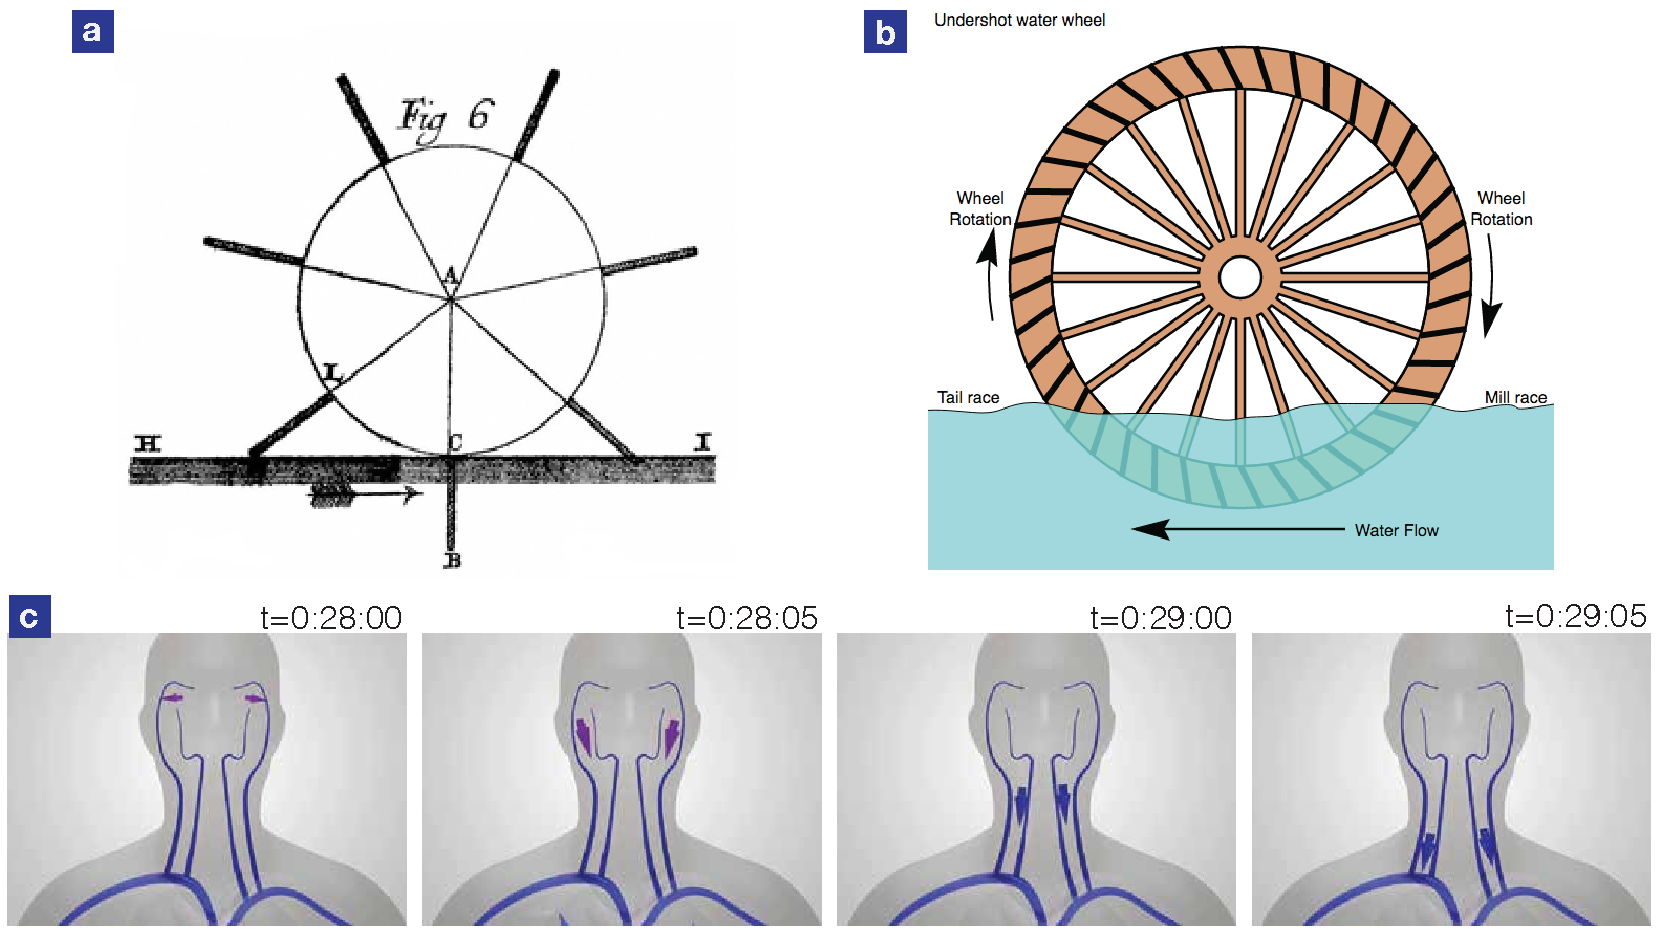
\includegraphics[width=\textwidth]{\intro/fig/arrows/arrows}
  \caption[Uses of motions arrows in visual instructions.]{Uses of motions arrows in visual instructions:
  %
  a) Year 1737: The first use of a motion arrow in an illustration explains the impact of water flow of a water wheel~\cite{de1737architecture},
  % http://www.buw-output-archiv.uni-wuppertal.de/ausgabe1/steinle/index-en.html
  %
  b) Year 2002: Similarly, arrows are used to explain the water flow and rotation of an undershot water wheel\footnote[1]{Original artwork by Daniel M. Short, ``Schematic diagram of an undershot water wheel'', licensed under CC BY-SA 2.5},
  % https://en.wikipedia.org/wiki/File:Undershot_water_wheel_schematic.svg
  %
  c) Year 2014: An animation visualizes the blood flow using motion arrows\footnote[2]{Video by Bioscience Credentials, ``Blood Flow in the Human Body'', \url{https://youtu.be/GwX41xm9esY}, licensed under CC BY 3.0}.
  }
  \label{fig:intro_arrows}
  \end{minipage}
\end{figure*}

Since the late 1990s, the advance in computer technologies has introduced more versatile instructional design. Instructions can now be created via software tools rather than hand drawing; they can include multimedia such as images and videos in several forms; they can be accessed through the Internet, as well as in hard copy.
%  the general purpose computers and the Internet
%
This advancement also enables consumers or end-users to document and share their domain knowledge~\cite{Lafreniere:2012tl}. As of today, popular tutorial sharing sites like Instructables has over 220,000 articles~\cite{InstructablesProjects}, wikiHow provides over 192,000 articles~\cite{wikiHowStatistics}, Food.com serves over 500,000 user-generated recipes with 125,000 photos~\cite{FoodComAbout}, and YouTube hosts over 285 million How-To videos\footnote{YouTube, \url{https://www.youtube.com/}, accessed June 2016}.
%
The variety of topics, content, and presentation styles provides learners more options to understand domain knowledge.
%
However, navigating a tutorial using existing tools remains inefficient for following step-by-step instructions. It can be challenging to observe details from text and images or find specific piece of information in a video through a timeline with conventional video players.
%
On the other hand, producing high-quality instructions that are easy to follow requires authoring expertise and a significant time investment. It involves several stages to design, record, and edit multimedia materials of a task using a variety of creation tools~\cite{Torrey:2007he,Tseng:2014:PVP:2598510.2598540,Muller:2009tw}.\\

The goal of this dissertation is to investigate interactive instructional design and develop computational tools that support the authoring process.
%
To contribute to computational methods of authoring user-generated instructions, two research questions that this work focuses on are:

\begin{itemize}
  \item How can authoring tools support domain experts in efficiently creating effective, high-quality instructions based on video-recorded demonstrations?
  \item How can new tutorial formats help authors better express their intent and help learners understand and follow the author's instructions?
\end{itemize}

This dissertation presents video-based computational approaches that enhance tutorial creation and consumption from author demonstrations.
We encode the current practices from professional authors into automatic algorithms and interactive techniques.
Our goal is to dramatically increase the quality of amateur-produced video instructions, which in turn improves learning for viewers who interactively navigate the content.
%
We will introduce five interactive systems that we develop to address these challenges. These tools cover both software applications (e.g., image manipulation tasks or browser navigation) and physical activities (e.g., Do-It-Yourself projects or dance movements) for recording, editing, and replaying instructional content.

% ---------------------------------------------------------------

\section{Challenges of Creating and Consuming Instructions}

Visual instructions are the dominant form of instructional design~\cite{mijksenaar1999open}. Cognitive load theory of multimedia learning suggests that learners process information using distinct channels, one for visual and the other for verbal formats~\cite{sweller1998cognitive,sweller1988cognitive,paas2003cognitive}. It was found that learners performed better when received a pictorial summary of a scientific system than those who received the full text alone or the full text with the summary~\cite{mayer1996less}.

Among all the multimedia support, videos are a common form to present instructions. We suspect that the great popularity of videos is due to the following reasons:
%
First, consumer devices and software have become affordable for authors to quickly record activities and later share via online platforms at minimum cost.
%
% ** describe the difficulties of making knowledge "explicit", esp. for actions and motions
Second, videos can be an efficient medium to document activities. Transferring know-how concisely and effectively to the audience is challenging. It especially requires efforts when a task involves \emph{tacit knowledge}, which is a kind of knowledge that is difficult to articulate in a written or verbal form~\cite{polanyi1958personal, Klemmer:2006:BMF:1142405.1142429}. Examples of tacit knowledge include dancing, riding a bike, or driving nails with a hammer. Dancers can perform movements fluently with music. If they are asked to focus on the composite pieces, such as the arm and foot actions or rhythm, they might get confused and fail to express the entire movement~\cite{polanyi1958personal}. Very often, recording a video eases the difficulties of describing the entire activities in an explicit form.
%
This leads to another motivation that videos also provide an effective channel to convey ideas with adequate amounts of details. Learners can visually observe the exact actions in a video as if an expert were coaching in person~\cite{Kuznetsov:2010:REA:1868914.1868950}.

However, while videos are easy to produce, they can include a lot of unnecessary footage. Inevitable content such as pauses, mistakes, and long repetitive actions makes it difficult for learners to focus on the most important steps and actions. A lot of authoring effort commonly goes into extracting footage, applying visual effects, and adding subtitles and annotations.
%
In addition, even with a well-edited video, navigating using a conventional video player remains inefficient. Learners with various needs could have a hard time skimming to an interesting moment or perceiving high-level overviews. Alternatively, a pictorial summary or static step-by-step tutorials presented with text and images can effectively guide knowledgeable learners through familiar tasks.

% The goal of this dissertation to develop video-based recording, editing, and playback tools are optimized for creating and consuming instructional demonstrations. I combine the advantage of ubiquitous video recording with the benefits of video and structured tutorial formats. I aim to dramatically increase the quality of amateur-produced video instructions, which in turn improves learning for viewers who interactively navigate the content.

% ----- MixT ----- %

\subsection{New Tutorial Formats}

Both static and video tutorials have strengths, but neither format alone is well suited for all learning needs that learners may have.
%
To combine the benefits, we design a new instructional presentation called \emph{MixT} (mixed-media tutorials) that improves learners' success in following instructions (see Figure~\ref{fig:mixt_intro}).
%
MixT presents step-by-step static instructions and includes in-place video clips for each operation.
%
With MixT, learners can quickly scan forward and backward on a web page to obtain an overview of a task. Embedded videos help them understand continuous, complex manipulation, such as brushing on a canvas and adjusting control points.
%
MixT's playback UI allows learners to interactively control \emph{when} to see images or videos, and \emph{how} to render videos.
%
Video editing techniques are applied to emphasize instructions, including cropping salient screen regions and highlighting interaction.
%
In our within-subject experiment, MixT successfully reduced numbers of errors and attempts made by learners when following image manipulation tasks.
% To demonstrate , MixT captures screencast video and operation events of a software demonstration.

\begin{figure*}[t]
  \centering
  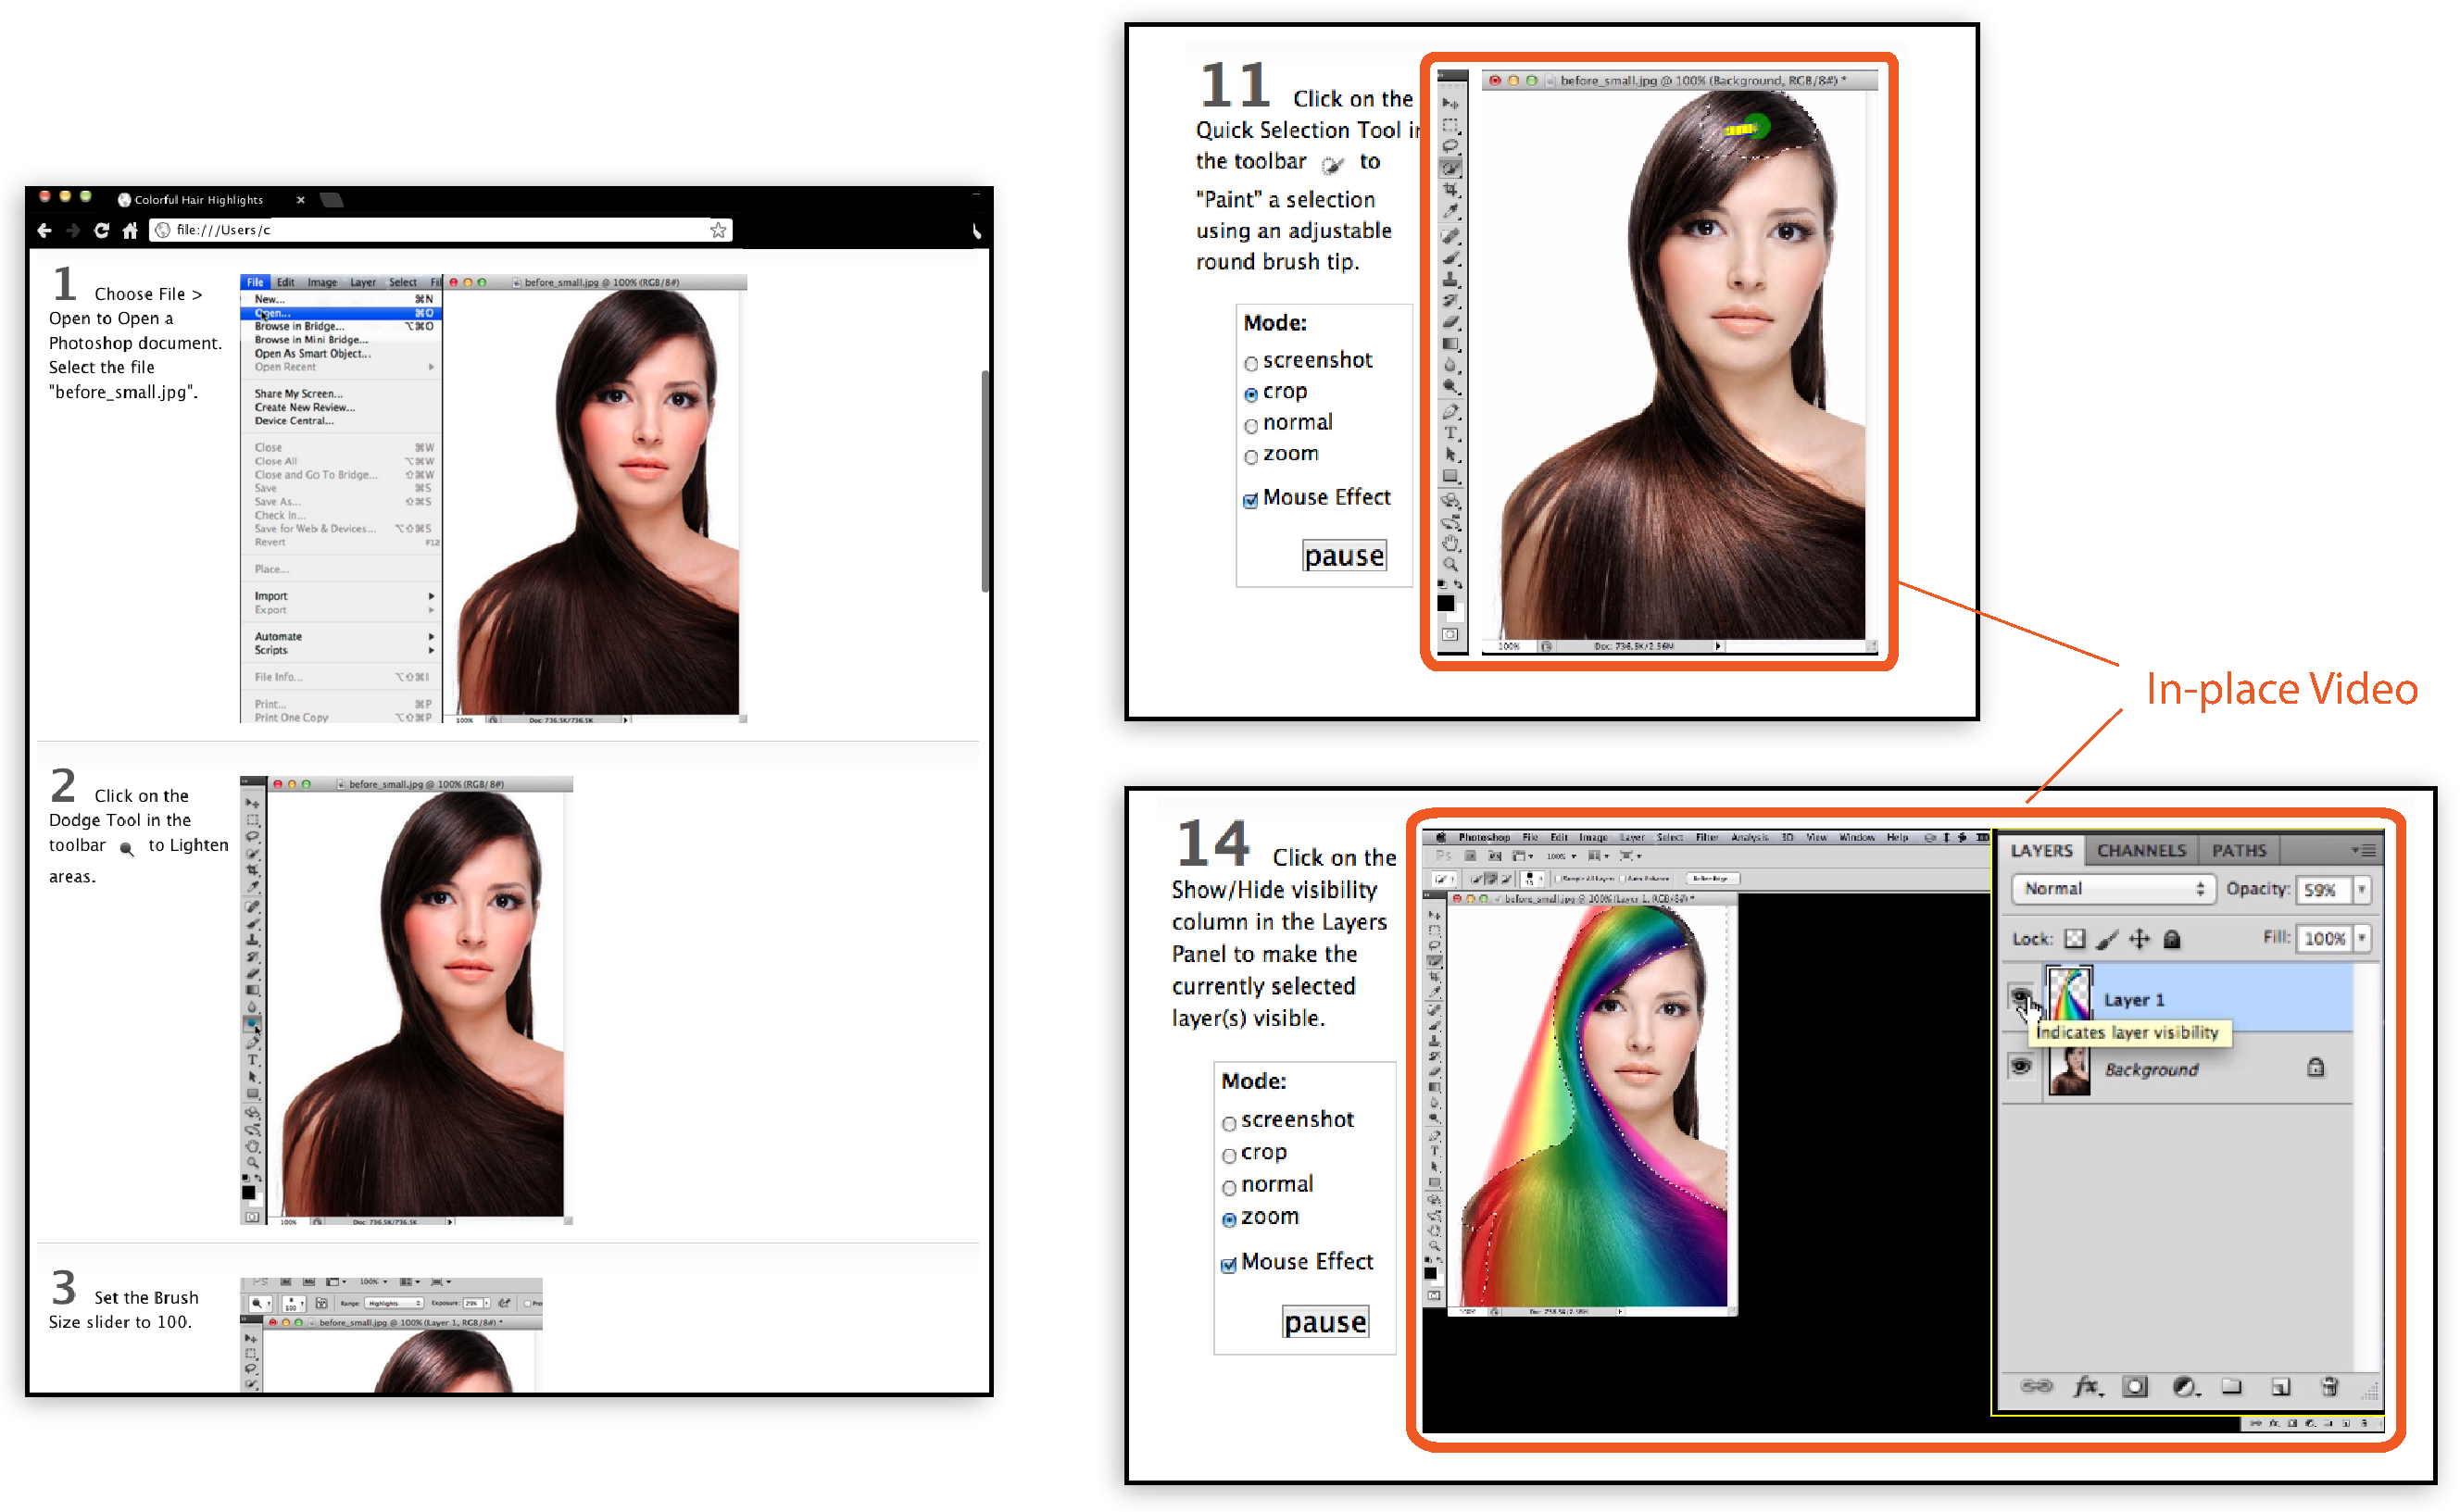
\includegraphics[width=0.8\textwidth]{\intro/fig/mixt_intro}
  \caption{MixT generates step-by-step tutorials (left) that contain static and video information from task demonstrations. Videos are automatically edited and offer different views (right) to highlight the most relevant screen areas for a step. Visualizing mouse movement helps learners understand a complex action.}
  \label{fig:mixt_intro}
\end{figure*}

% ----- DemoWiz ----- %
MixT offers a novel way of navigating instructional content with a combination of static step-by-step and embedded video presentations. If an author wants to narrate over a video recording to illustrate a demo, it can be challenging to pace oneself at the suitable timing without expecting \emph{when} and \emph{what} action is taking while a video is playing.
%
We design \emph{DemoWiz}, a system that augments a screencast video with visualizations (Figure~\ref{fig:demowiz_intro}). By logging the input events of a software demonstration, DemoWiz overlays glyphs to visually guide viewers to the next action along with the time remaining before the action occurs. This enables viewers to anticipate the video content rather than react to it.
%
Our study showed that fewer anticipation errors and narration delays were made with DemoWiz.

\begin{figure*}[t]
\centering
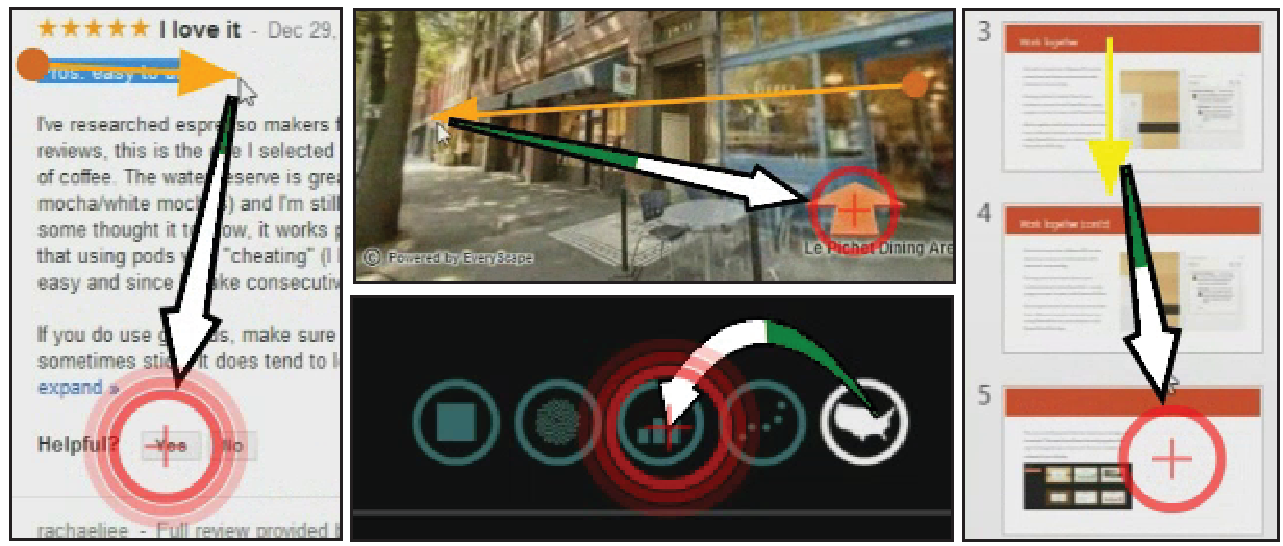
\includegraphics[width=0.7\columnwidth]{\intro/fig/DemoWiz}
\caption{DemoWiz visualizes input events in a screencast video to help viewers anticipate the upcoming event for following a software demonstration.}
\label{fig:demowiz_intro}
\end{figure*}

\subsection{Tutorial Generation from Software Demonstration}

While new tutorial formats are shown to be useful, manually creating instructions can be extremely time- and effort-consuming. In response, we design computational methods to automate the creation process from an author demonstration. MixT and DemoWiz capture screencast video and input device events from a demonstration of a task in a software application. MixT also records application commands for video analysis. Computer vision and visualization techniques are integrated to segment a video into steps, extract salient information, and add visual highlights.
%
In addition, DemoWiz supports an editing phase where authors can adjust the timing of events in a video. Playback speed of recorded actions can be modified or skipped via an editing UI. Our studies showed that our algorithms for step segmentation, event detection, and visualization were effective (\textless8\% error rate in MixT and 0\% in DemoWiz).

\subsection{Interactive Tutorial Authoring from Physical Demonstration}

% ----- DemoCut ----- %

Moving beyond software applications, support for authoring instructions of tasks that take place in the physical world is lacking. Activity recognition remains an open research question, and making authoring decisions during a demonstration can be difficult.
%
To address this problem, we first look into Do it yourself (DIY) project tutorials, which help people learn knowledge and skills to complete a task independently.
%
We developed \emph{DemoCut}, a semi-automatic video editing system that improves the quality of amateur instructional videos for physical tasks (Figure~\ref{fig:democut_intro}). DemoCut asks authors to describe key ``moments'' in a recorded demonstration video using a set of markers. Based on the annotations, our system analyzes the audio and visual activities to automatically organize the video into meaningful segments. Editing decisions are applied to support both \emph{temporal effects} that increase playback speed or skip segments, as well as \emph{visual effects}, such as zooming, subtitles, and visual highlights. A playback interface allows authors to quickly review and edit the automatically generated effects.
%
Our studies showed that video tutorials created by DemoCut in five DIY domains were concise in terms of video length and descriptive instructions with low effect error rates.

\begin{figure*}[t]
  \centering
  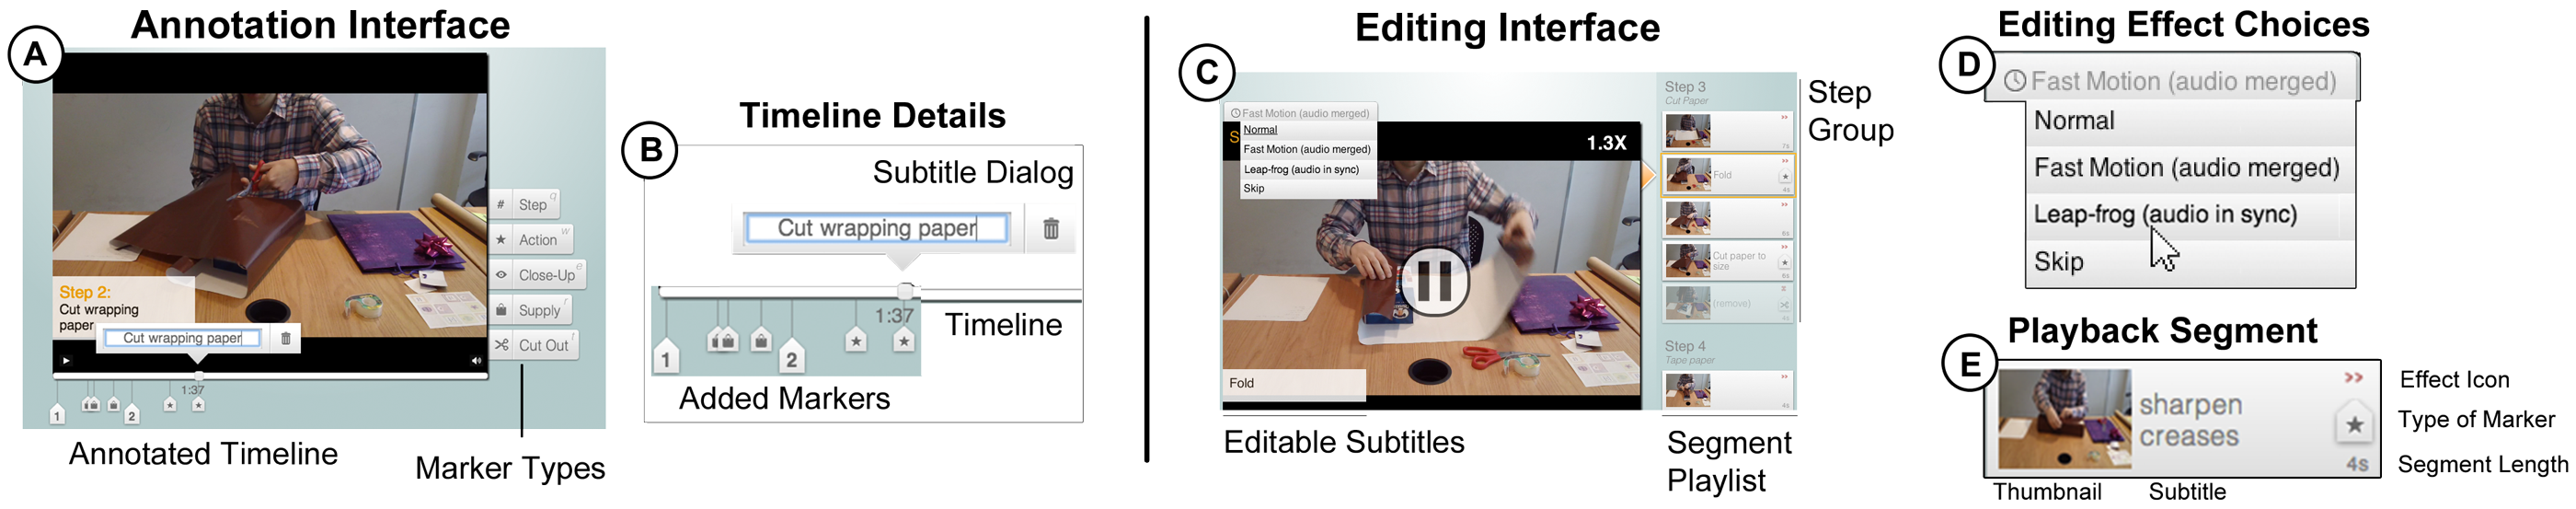
\includegraphics[width=\textwidth]{\intro/fig/DemoCut}
  \caption{DemoCut asks authors to mark key moments in a recorded video of demonstration using a set of marker types. Based on marker information, the system uses audio and video analysis to automatically organize the video into meaningful segments and apply appropriate video editing effects, which can be modified via a playback UI.}
  \label{fig:democut_intro}
\end{figure*}

% ----- Kinectograph ----- %
Through the process of designing DemoCut for automatic DIY video editing, we observed that for tasks that require larger space and more movements, instructors often have to adjust the position and viewing angle of a camcorder. Some authors choose to set up multiple cameras and later select the best shot from video streams, while some invite another person who controls the camcorder during a demonstration.
%
To enable authors to record their demonstration without acquiring additional cameras or cameraman, we design \emph{Kinectograph}, a video recording device with a single camera that automatically tracks and follows specific body parts, e.g., hands, of an instructor in a video (see Figure~\ref{fig:kinectograph_intro}). It utilizes a Kinect depth sensor to track skeletal data and adjusts the camera angle via a 2D pan-tilt gimbal mount. Authors can freely move around in space to demonstrate a task and monitor real-time video preview through a tablet application.

\begin{figure}[!t]
  \centering
  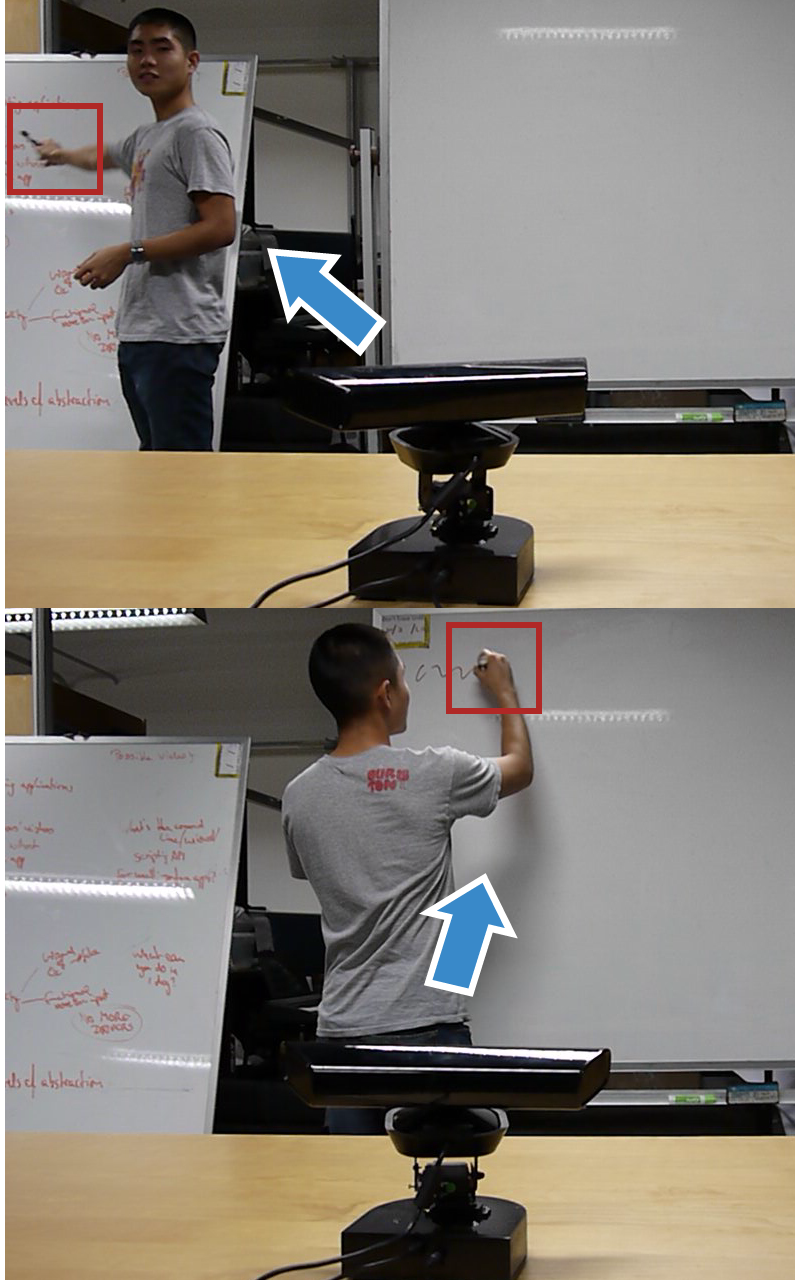
\includegraphics[width=0.65\columnwidth]{\intro/fig/Kinectograph}
  \caption{Composed of a Kinect camera to track author movement and a motorized dock to pan and tilt the camera, Kinectograph allows the author (or their hand) remains centered in the recorded video in real-time.}
\label{fig:kinectograph_intro}
\end{figure}

% ----- DemoDraw ----- %

The successful experiences supporting motion-based recordings motivated me to apply our demonstration-based approach to a domain that is entirely driven by movements. In sports, dance performance, and body gesture interfaces, movement instructions are often conveyed with drawings of the human body annotated with arrows or stroboscopic effects~\cite{cutting_representing_2002}. However, current practices require authors to manually sketch or trace subjects from photographs, which is time-consuming and difficult to make changes once created.
%
We design \emph{DemoDraw}, a system that generates concise illustrations from author demonstration (see Figure~\ref{fig:demodraw_intro}). With DemoDraw, an author records one or more motions by physically demonstrating in front of a Kinect sensor. In a multi-modal Demonstration Interface, DemoDraw segments speech and 3D joint motion into a sequence of motion segments, each characterized by a key pose and salient joint trajectories. Based on this sequence, a series of illustrations is automatically generated using a stylistically rendered 3D avatar annotated with arrows to convey movements. Once a suitable sequence of steps has been created, a Refinement Interface enables fine control of visualization parameters.
%
In a three-part evaluation, our results show 4 to 7-step illustrations can be efficiently created in 5 or 10 minutes on average.

\begin{figure}[t]
  \centering
  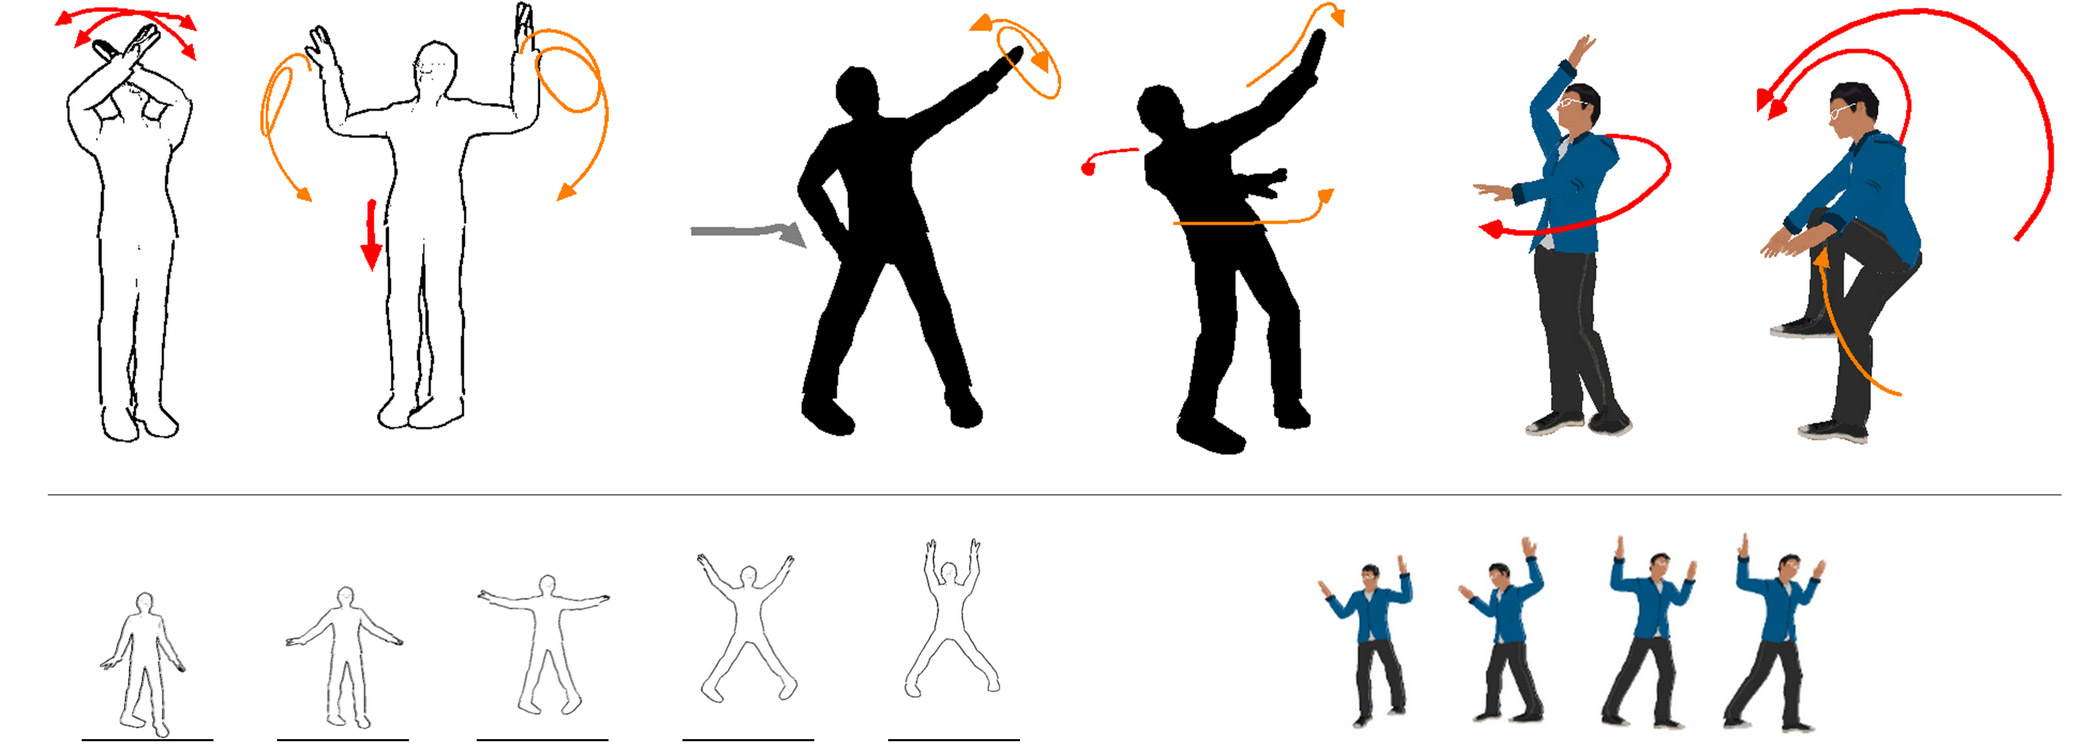
\includegraphics[width=\columnwidth]{\intro/fig/DemoDraw}
  \caption{DemoDraw's multi-modal approach enables authors to capture motion, verify results, and re-perform portions if needed to generate step-by-step motion illustrations.}
  \label{fig:demodraw_intro}
\end{figure}

% ---------------------------------------------------------------

\section{Thesis Contributions}

Overall, our video-based approaches consider key events or moments that are important to a learner. This information can be derived from software event logs or human annotation of physical tasks when automatic recognition remains challenging. Based on the metadata and video streams, we propose automatic methods to generate concise instructions for two task domains, software applications and physical tasks (see Figure~\ref{fig:space}). Our approaches support authors from recording demonstrations to editing and reviewing system-generated instructions. Interactive controls are available in different stages via desktop or multi-modal interfaces.
%
We demonstrate a series of systems that consider production stages of tutorial creation and learning. We present the rationale and technical challenges of these interactive system designs. Each system is evaluated both quantitatively and qualitatively to study the usability in authoring and learning.

\clearpage
The contributions of this dissertation include:

\begin{itemize}
\item New instructional formats that consider the learning needs from several domains, including software applications and physical activities.
\item Multi-modal interaction techniques for novice or amateur authors to create effective instructions by demonstration.
\item Automatic or semi-automatic approaches using video and audio analysis that includes authors in the loop to produce high-quality instructions.
\end{itemize}

\begin{figure}[t!]
  \centering
  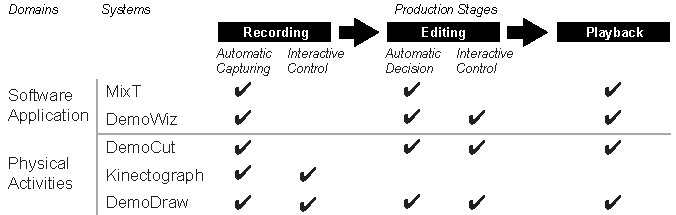
\includegraphics[width=0.9\columnwidth]{\intro/fig/space}
  \caption{A design space of the creation and consumption process for tutorials. It involves three phases of recording, editing, and playback in either software domain or a physical world. This dissertation proposes a series of systems that focus on various aspects in this design space.}
  \label{fig:space}
\end{figure}

% ---------------------------------------------------------------

\section{Overview}

The rest of this dissertation is structured as follows:
%
In Chapter \ref{chapter_background}, we define terminology used in instruction creation and consumption process based on literature. We review studies on why people rely on tutorials in general, how the formats of instructions matter, and the current practices of authoring instructions.
%
In Chapter \ref{chapter_related_work}, we review the literature on research and technologies used in supporting activities of authoring and consuming instructions.

We presented two systems that generate interactive tutorials for software applications.
% MixT
In Chapter \ref{chapter_mixt}, we present our study on how a new tutorial format supports learners in following step-by-step instructions with mixed media, including static text, images, and video clips. We introduce our creation tool called MixT, which automatically generates such new tutorial format from a software demonstration.
% DemoWiz
Chapter \ref{chapter_demowiz} introduces DemoWiz, a system that assists viewers in capturing the timing of input events in a screencast demo video. DemoWiz supports recording, editing, and reviewing stages in a production process with an authoring and playback UI.

Then, we introduced three systems designed for real-world tasks that involve physical demonstrations.
% DemoCut
In Chapter \ref{chapter_democut}, we present a semi-automatic tool for DIY video editing. Our system, called DemoCut, provides two authoring interfaces, annotation and editing, that enable authors to mark a demo video and review and modify the automatically edited results. The design is based on an fundamental understanding of DIY activities.
% Kinectograph
In Chapter \ref{chapter_kinectograph}, we focus on a recording device that automatically follows a demonstrator for filming instructional videos. The Kinectograph system tracks an author's position and body parts and provides an authoring interface for real-time camera control.
% DemoDraw
Finally, in Chapter \ref{chapter_demodraw}, we introduce a multi-modal approach for authors to generate motion illustrations by physically demonstrating the movements. DemoDraw is a system that segments speech and 3D joint motion into a sequence of motion segments and renders effective illustrations. Two authoring interfaces enable authors to navigate, re-perform, and edit visualization parameters.

% Conclusion
Throughout this dissertation, we discuss how our video-based approaches increase the quality of amateur-produced video instructions. Chapter \ref{chapter_conclusion} concludes our work on tutorial creation and consumption in both software and physical instructions. New directions for future research on interactive tutorials are proposed.

% ---------------------------------------------------------------

\section {Prior Publications}

This dissertation is based on papers published in previous ACM conference proceedings: the MixT system was published at UIST 2012~\cite{Chi:2012:MAG:2380116.2380130}, DemoWiz at CHI 2014~\cite{Chi:2014:DRS:2556288.2557254}, DemoCut at UIST 2013~\cite{Chi:2013:DGC:2501988.2502052}, and Kinectograph at CHI 2013~\cite{Cheng:2013:BCC:2468356.2468568}; DemoDraw will be published at UIST 2016~\cite{Chi:2016:DemoDraw}.

While I am primary author on all publications and led the described projects, this research could not have been completed without my advisor Bj\"orn Hartmann and my collaborators that I have been fortunately to work with. Specifically, Dr. Mira Dontcheva and Dr. Wilmot Li at Adobe Research provided valuable guidance on three projects (MixT, DemoCut, and DemoDraw); Dr. Steven M. Drucker and Dr. Bongshin Lee at Microsoft Research guided the DemoWiz project with their expertise on visualization; Professor Daniel Vogel at University of Waterloo greatly contributed to the DemoDraw project. A group of MS and undergrad students at UC Berkeley and Adobe contributed to implementation, design, and user study in the projects, including Sally Ahn and Amanda Ren in MixT, Joyce Liu and Jason Linder in DemoCut, and Derrick Cheng and Taeil Kwak in Kinectograph.

% We are all natural performers. Humans are proficient at demonstrating how to perform a task in action. However, articulating knowledge into a written or structured form can be extremely difficult. From dancing, repairing a machine, to operating software applications, it remains a challenge how everyday activities can be efficiently captured for a remote learner to understand.

%!TEX root = ../thesis.tex
% This paragraph covered a lot of ground, but I was a bit lost since each sentence tried to cover too many different approaches. Is there an implied structure? E.g. first software-static, then software-video, then physical tasks? Id’ have expected some more basic references early on that for example show that people don’t read software documentation and instead look for task-centered learning materials. There’s also a difference between related work that investigates what good instruction formats are, and systems work that introduces new tools to create such formats.

% add some Tiffany Tseng's work
% http://web.mit.edu/ttseng/www/academics/index.html

\chapter {Background}
% This section presents the state-of-the-art of technologies that support tutorial authors and learners.
The research community has been investigating the motivations of both authors and viewers of how-to videos and written tutorials. While one primary motivation is to share expertise, published videos also serve as a way to broadcast skill and as an online portfolio~\cite{Torrey:2007he,Kuznetsov:2010:REA:1868914.1868950}. Authors may derive revenue through advertising or referrals~\cite{Lafreniere:2012tl}. Viewers, on the other hand, typically seek technical explanations, but are also searching for inspiration~\cite{Torrey:2009fc} and looking for validation of existing skills~\cite{Lafreniere:2012tl}.
%
These studies suggest that tutorials have a larger variety of purposes and uses than merely communicating technical content. Recently, guidelines of improving tutorial authorship have been proposed \cite{Wakkary:2015:TAH:2702123.2702550}. Key findings include identifying tools and components and structuring a task into steps with a clear sequence. In our work, we strive to make authoring of instructions more accessible to amateurs while maintaining opportunities for adding individual style through control over editing effects.

% -------------------------------------------

\section{Help and Instruction Formats}
There has been a considerable amount of research devoted to tutorial designs that help viewers operate an interactive system. Efforts include visualizing events or embedding instant assistance in software applications and providing real-time feedback on physical tasks.

\subsection{Software Visualization}
In the software application domain, visualizing input and output events has shown to be effective in enhancing instructions. Events can range from low (e.g., mouse actions and movements or keyboard strokes) to high level (e.g., UI component changes). Examples include rendering markers and arrows on screenshot images of a software demo process \cite{Nakamura:2008:ASV:1449715.1449721, Grabler:2009jj}, automatic indexing of instructional software videos \cite{Banovic:2012kd}, and providing visual feedback based on UI operations in real-time \cite{Dixon:2010fb,Dixon:2011:CHP:1978942.1979086}. Work has also aimed to visualize application-centric processes, such as 3D mesh construction \cite{Denning:2011fy} or image manipulation tasks \cite{Grabler:2009jj} as a step-by-step list.

\subsection{In-Application Support}

Another approach is to provide in-application assistance, often in real-time, in a specific context. Methods include embedding video snippets in application tooltips \cite{Grossman:2010wr}, providing step-by-step wizards \cite{Bergman05docwizards:a,Kelleher:2005:STD:1054972.1055047,Fernquist:2011:SRE:2047196.2047245}, automatically navigating video tutorials based on user operations \cite{Pongnumkul:2011ju}, and showing a history of before and after thumbnails and video clips \cite{Grossman:2010jz}. In-app supports can also be dynamically updated within a community based on user contribution \cite{Lafreniere:2013ff,Matejka:2009:CCR:1622176.1622214}.

\subsection{Instructions for Physical Tasks}

Beyond software applications to the real world where activity and object recognition is difficult, researchers have investigated tools for supporting physical tasks. Workflows can be automatically generated for furniture \cite{agrawala2003designing} or block assembly tasks \cite{Gupta:2012ku}; the latter was shown to be trackable for real-time guidance.
%
Information can also be overlaid on top of the work area using augmented reality, usually through a head-mounted display. Such systems can provide visual highlights for machine maintenance \cite{Henderson:2011ff}, or interactive remote tutoring for repair tasks~\cite{Gurevich:2012ko}. Another method is to overlay guidance on an augmented mirror for tasks such as dance movements \cite{Anderson:2013:YEM:2501988.2502045}.

These projects show how effective instructional representations can assist learners in learning or executing tasks. Our goal is to further study new formats that incorporate advantages of several formats of multimedia, including images, text, and videos, and in turn enhancing the learning experience for a variety of tasks.

% -------------------------------------------

\section{Activity Tracking}
To provide real-time assistance, it is important to recognize the user activities during a task performance. Several domains have been widely studied, including software operations, scene recognition, and object tracking in a physical world.
%
Researchers have shown that workflows and content of desktop applications can be captured automatically using computer vision \cite{Yeh:2009dh,Chang:2011vd} and application logs \cite{Grossman:2010jz,Grabler:2009jj,Pongnumkul:2011ju}.
%
However, tracking user behavior in the physical world, rather than in software, remains a challenge. Computer vision techniques can track specific targets, including hands \cite{Ranjan:2008}, user movements \cite{Wilson:2012fb}, fast-moving objects (e.g., a Ping-Pong ball) \cite{Okumura:2011tr}, or regions in pre-defined spaces \cite{Ranjan:2007}.

These methods usually require an expert defining heuristics of space regions or movement classifications ahead of time for the tracking program.
%
On the contrary, we propose a new approach that does not have these issues, gives users flexibility in a home environment, and provides interactive control. If activity recognition is not possible, we include users in the loop to annotate high-level information in order to create high-quality results.
%
Emerging work has provided insights toward this vision using consumer devices such as a Kinect sensor \cite{Anderson:2013:YEM:2501988.2502045,Gupta:2012ku} to provide dynamic instructions, which shares a similar goal with ours.

% -------------------------------------------

\section{Video Capture, Annotation and Editing}
% \subsubTitleI{Capture} Several research and commercial systems guide users at capture time to yield higher-quality videos. Such systems often employ templates to help users capture sequences of distinct shots (e.g., Snapguide\footnote{http://snapguide.com/}) or suggest framing of the subject or camera view as in NudgeCam~\cite{Carter:2010}. Computer vision algorithms, like face tracking, can be used to offer real-time feedback during such directed actions~\cite{Davis:2003cu,Heer:2004ba,Carter:2010}. Instead of relying on templates, shot suggestions can also be bootstrapped through user dialogs~\cite{Adams:2005}.

% \subsubTitleI{Annotation} Researchers have investigated how to provide interactions that enable efficient, fluid annotation of video data, from the early EVA system~\cite{Mackay:1989} to more recent interfaces like VideoTater that leverage pen input~\cite{Diakopoulos:2006vt}. We do not claim a contribution in the interaction techniques of our annotation interface and take inspiration from such prior work.

% \subsubTitleI{Editing} Frame-based editing of video is very time-intensive, as it forces users to operate at a very low level of detail. Editors can leverage metadata, such as transcripts~\cite{Berthouzoz:2012,Pavel:2014:VDB:2642918.2647400} and shot boundaries~\cite{Casares:2002dx}, to give users higher-level editing operations at the shot level rather than the frame level.
%In specific video domains like interview videos, transcripts can help users place cuts and transitions~\cite{Berthouzoz:2012}.
Computer vision techniques can automate certain effects, such as creating cinemagraphs~\cite{Bai:2012, Joshi:2012}, automatically-edited lecture videos~\cite{Heck:2007}, zoomable tapestries~\cite{Barnes:2010} and synopses~\cite{Pritch:2009vl}, or stabilizing shaky amateur videos~\cite{Liu:2011}. When analyzing video is a matter of subjective taste, identifying salient frames can also be outsourced to crowd workers~\cite{Bernstein:2011uj}.

In contrast to these systems, we do not require the author to manipulate the camera or system during capture. Many leisure activities, such as home repair or cooking, require use of both hands or involve getting one's hands dirty, so camera manipulation is not possible. We use vision techniques for automatic recording and editing. It differs from previous approaches in its focus on particular application domains -- software and physical demonstrations. By focusing on specific domains, we can make assumptions about the structure of the input and output video, such as the fact that there is a linear set of steps or movements, and offer user interfaces and algorithms that make it easier to create high quality instructions.

%!TEX root = ../thesis.tex

\chapter{Related Work}
\label{chapter_related_work}

While existing practices require tutorial authors to create instructions manually, HCI and Computer Graphics communities have introduced novel technologies for authoring tutorials, including automatic generation methods and interactive editing tools.
%
In this chapter, I survey state-of-the-art techniques for generating instructions for both software applications (Section \ref{related_software}) and physical tasks (Section \ref{related_physical}).
%
Furthermore, existing instructions are mainly offered in the forms of conventional media, such as static tutorials (print-outs or web) or videos. With software systems, \keyword{interactive tutorials} have been introduced for learners to interactively review instructional content. I will discuss various forms of such kind of instructions by prior research, which leads to a discussion on the remaining gaps in tool support for creating and navigating instructional content.

% -------------------------------------------

\section{Instructions for Software Applications}
\label{related_software}

\subsection{Workflow Capturing and Tutorials}

Revealing operation history has shown to be effective in presenting software instructions. Operational events can range from low-level, application agnostic input device events (e.g., mouse actions, cursor movements, or keyboard strokes) to higher level, application-dependent information (e.g., menu selections or UI component changes).
%
Researchers have investigated automatic approaches that capture and visualize these types of events. Nakamura and Igarashi~\cite{Nakamura:2008:ASV:1449715.1449721} proposed a capturing and rendering system independent to GUI applications. Their system logs mouse events of a software demonstration process, including mouse moving, dragging, and clicking. Operations are rendered as markers and arrows on screenshot images to present the linear event history (see Figure~\ref{fig:related_events} top).
%
Grabler \ea{}'s approach~\cite{Grabler:2009jj} further analyzes the application context, including facial features and outdoor scenes, and annotates software screenshots with arrows, bounding boxes, and call-outs (see Figure~\ref{fig:related_events} bottom). In addition to annotated images, their system generates textual description from templates, such as \iquote{Select the \textbf{path tool} from the \textbf{toolbar} to \textbf{create and edit paths}.} The generated text and rendered images of operations are presented as a step-by-step tutorial, which is currently available as a Photoshop plug-in\footnote{Adobe labs. Tutorial Builder. \url{http://labs.adobe.com/technologies/tutorialbuilder/}}.

Demonstration-based approaches for generating instructions have been also applied to applications that involve more complicated manipulations or gestures, including 3D mesh construction~\cite{Denning:2011fy} and mobile apps~\cite{Wang:2014:EAC:2556288.2557407}.
%
Beyond logging events from recording a user demonstration, researchers have shown that workflows and software content can be captured automatically using application logs \cite{Grossman:2010jz,Grabler:2009jj,Pongnumkul:2011ju} or computer vision from analyzing desktop regions~\cite{Yeh:2009dh,Chang:2011vd} and existing screencast videos~\cite{Banovic:2012kd}.

\begin{figure*}[t!]
  \centering
  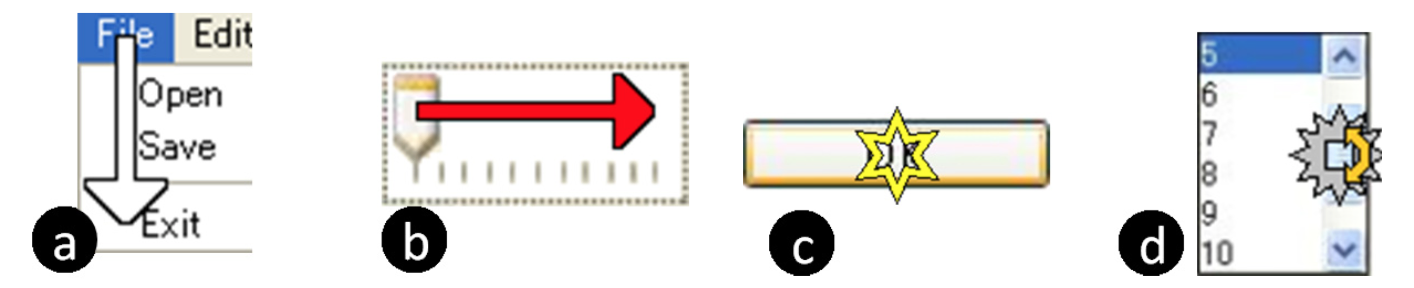
\includegraphics[width=0.6\textwidth]{\background/fig/software_viz/Nakamura_and_Igarashi}
  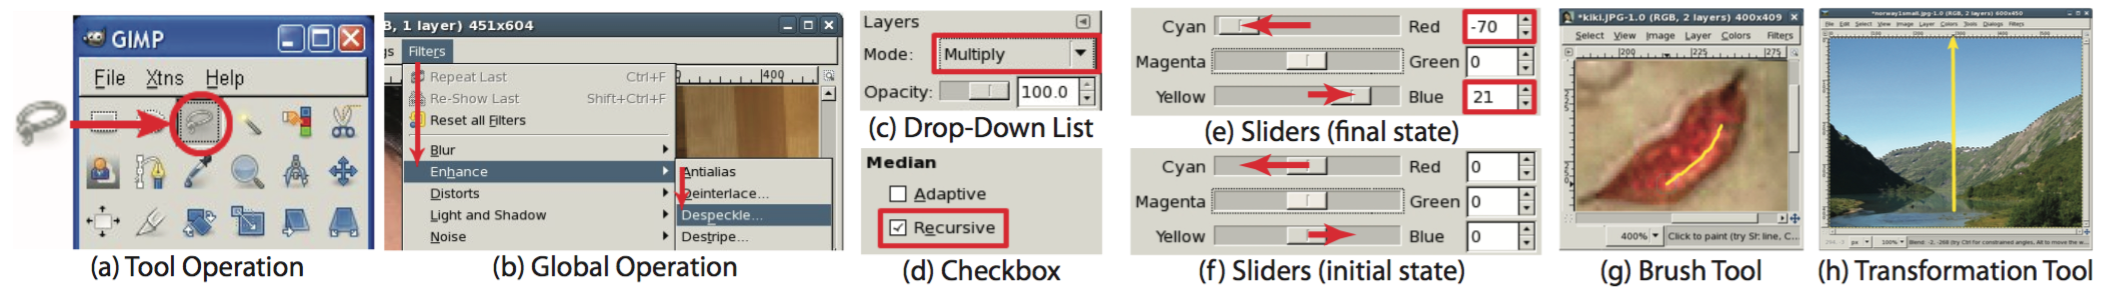
\includegraphics[width=\textwidth]{\background/fig/software_viz/Grabler}
  \caption{Example screenshots that visualize mouse operations are automatically rendered, including (top) mouse move, drag, click, and wheel (a-d) by Nakamura and Igarashi~\cite{Nakamura:2008:ASV:1449715.1449721} and (bottom) application-specific operations (a-b), parameters (c-f), and manipulations (g-h) by Grabler \ea{}~\cite{Grabler:2009jj}.}
  \label{fig:related_events}
\end{figure*}

To compare operation effects and workflows, other effective visualization approaches include showing a list of ``before'' and ``after'' thumbnails, video clips, and event timeline \cite{Grossman:2010jz} and creating a union graph of operations \cite{Kong:2012:DTR:2207676.2208549} (see Figure~\ref{fig:related_comparison}).

\begin{figure*}[t!]
  \centering
  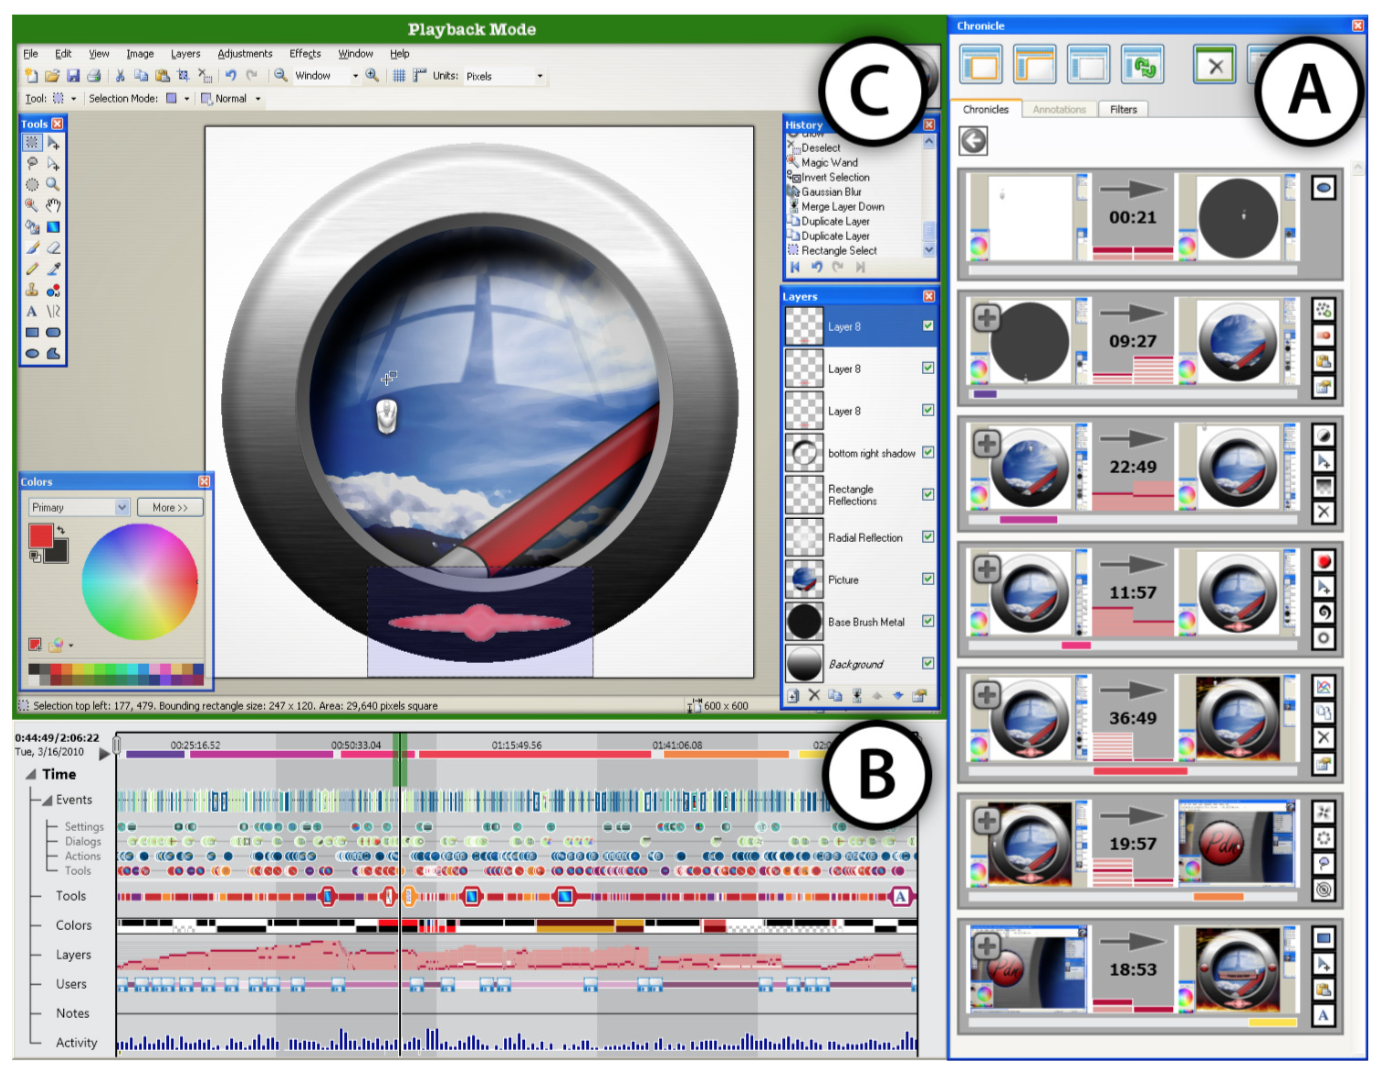
\includegraphics[width=0.4\textwidth]{\background/fig/software_viz/Grossman}
  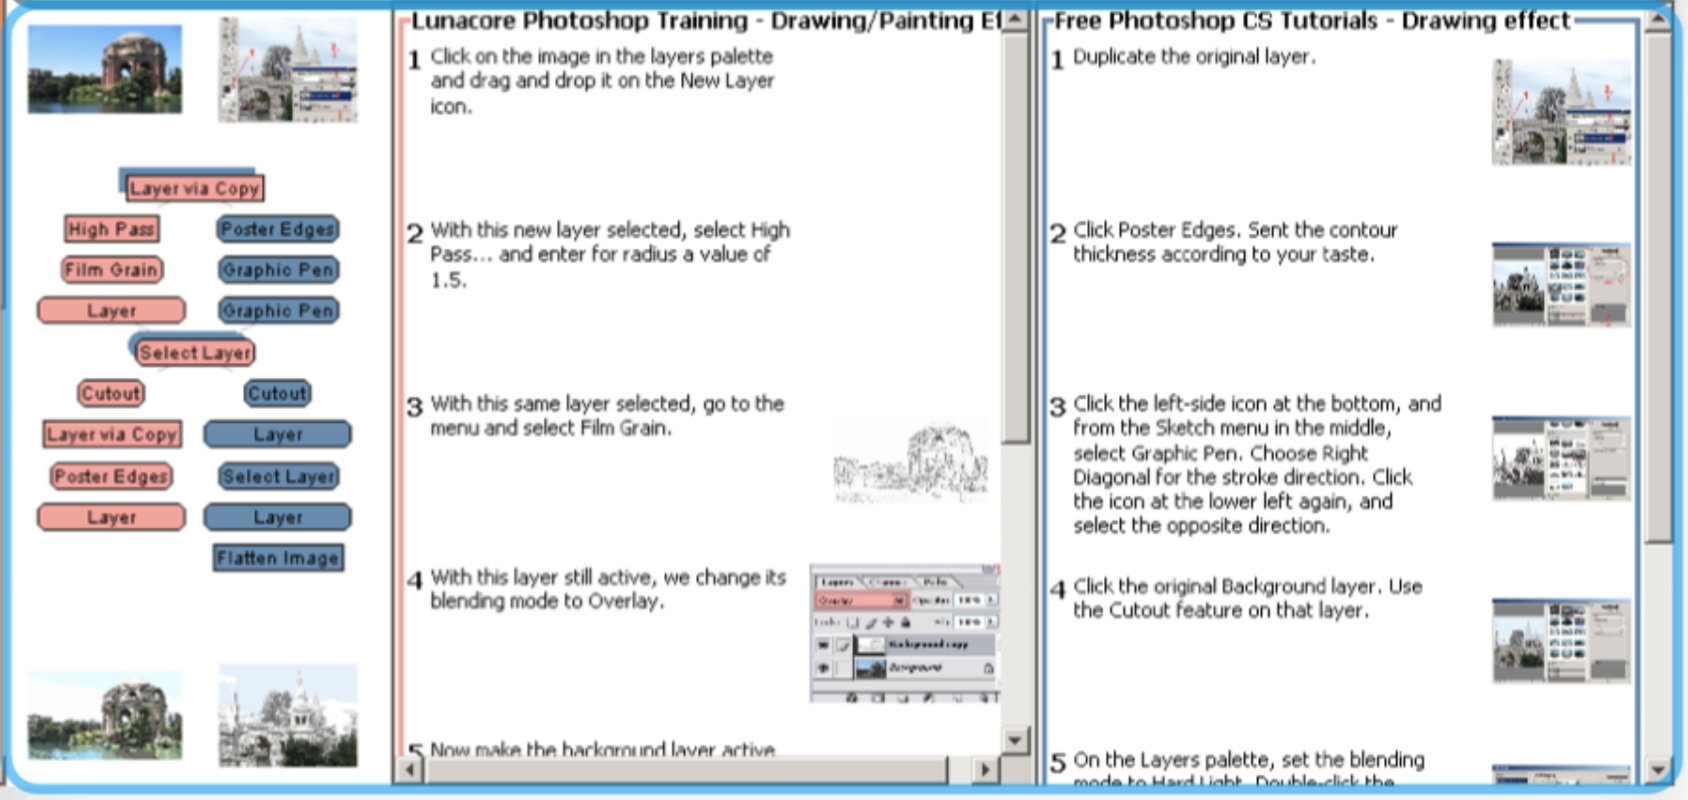
\includegraphics[width=0.55\textwidth]{\background/fig/software_viz/Kong}
  \caption{Instructional systems that help learners compare effects and similar tutorials using: (left) before and after images (a) and event timeline (b) by Grossman \ea{}~\cite{Grossman:2010jz} and (right) operation union graph by Kong \ea{}~\cite{Kong:2012:DTR:2207676.2208549}.}
  \label{fig:related_comparison}
\end{figure*}

% -------------------

\subsection{In-Application Support}

The above systems introduce innovative ways of providing informative screenshots or representations for learners to review workflows. However, reviewing these materials is often separated from operating a software application. Learners might have to switch between context of interacting an application and reading instructions, which could introduce a gap of evaluation (\iquote{Am I doing this right as the instructions explain?}) and a gap of execution (\iquote{How do I perform the action that the instructions describe?}).
%
Researchers have proposed another approach to provide ``in-application'' assistance, often in real-time, in a specific application context.

Studies have shown that visualizing input events in real-time during operations can provide better learnability of applications \cite{Dixon:2010fb}.
%
Commercial tools such as Mouseposé\footnote{Mouseposé \url{http://www.boinx.com/mousepose}} and ScreenFlow\footnote{ScreenFlow \url{http://www.telestream.net/screenflow}} visualize mouse and keyboard events with special effects, such as drawing a circle around a mouse cursor (see Figure~\ref{fig:related_realtime} top).
%
Dixon \ea{} proposed techniques to provide pixel-based enhancements in real-time, such as highlighting nearest regions of interest or applying afterglows based on the current user operations \cite{Dixon:2010fb,Dixon:2011:CHP:1978942.1979086} (see Figure~\ref{fig:related_realtime} bottom).

\begin{figure*}[t!]
  \centering
  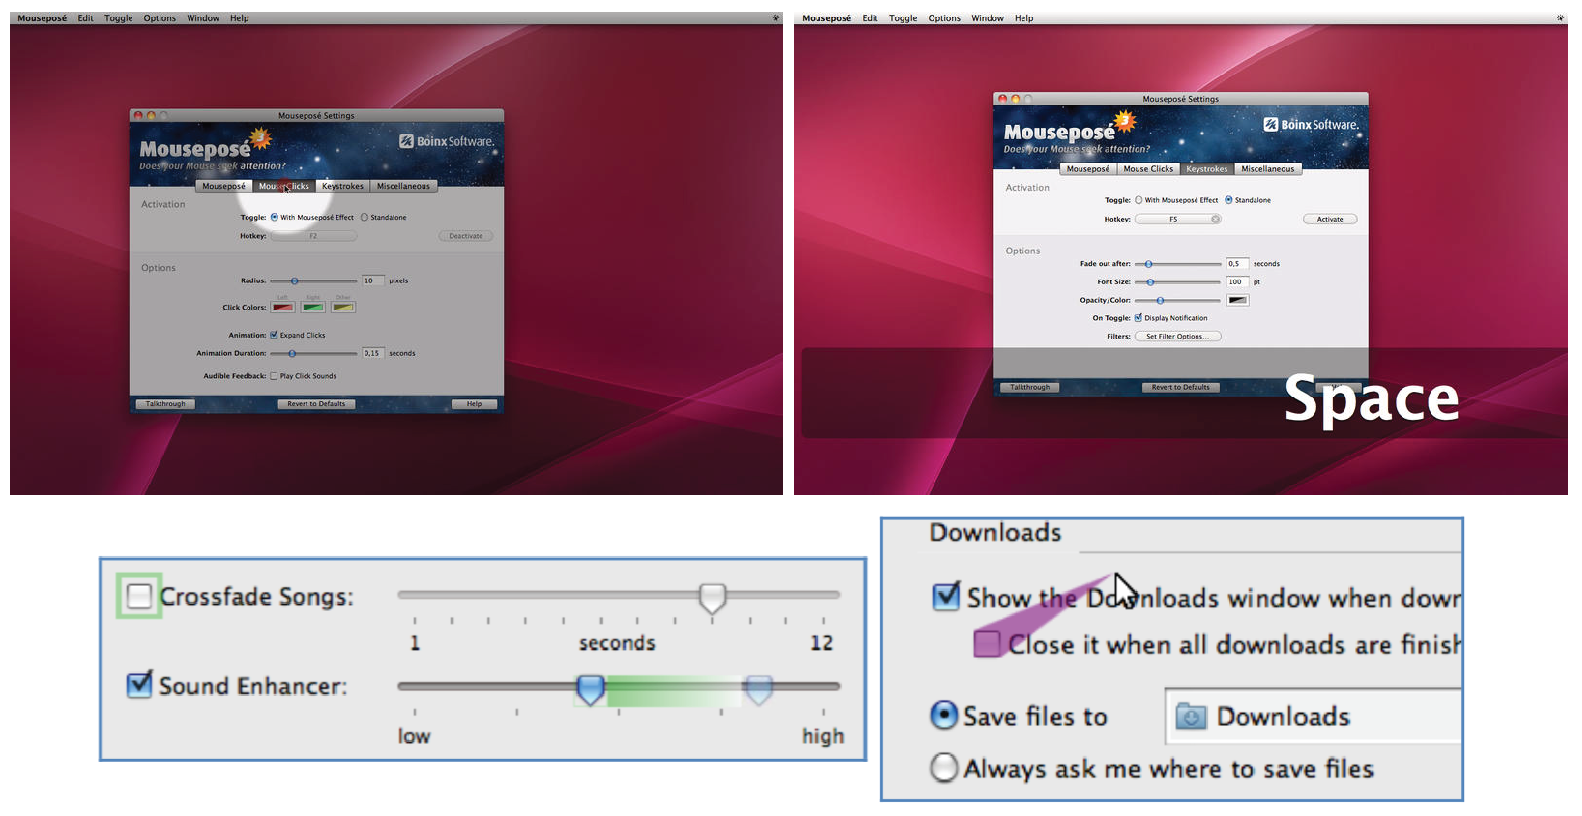
\includegraphics[width=0.7\textwidth]{\background/fig/realtime/realtime}
  \caption{Real-time visual enhancements on GUI applications: (top) Mouseposé highlights mouse cursors or text input; (bottom) Prefab creates target-aware or afterglow effects during user operating~\cite{Dixon:2010fb}.}
  \label{fig:related_realtime}
\end{figure*}

Real-time visual effects help users focus on the region of interest in a GUI application, but to support learners comprehend the application functionalities, there has been a considerable amount of research devoted to offering interactive helps.
%
Video snippets can be embedded in application tooltips~\cite{Grossman:2010wr}, which were shown to be seven times more effective than conventional tooltips for completing unfamiliar tasks.
%
Interactive, step-by-step instructions can be integrated in several forms:
%
To help user identify the correct UI components, tutorials can be shown via translucent colored ``stencils,'' which visually direct user's attention directly in an application~\cite{Kelleher:2005:STD:1054972.1055047}.
%
By tracking user's current operations, tutorials can be embedded in an application to provide instant feedback such as a check-mark or a percentage match~\cite{Fernquist:2011:SRE:2047196.2047245}, automatically replayed to provide the corresponding video instructions~\cite{Pongnumkul:2011ju}, or be shown as ambient help~\cite{Matejka:2011:AH:1978942.1979349}.
%
Instructions can be captured from demonstration as ``scripts'' for step-by-step navigation~\cite{Bergman:2005:DocWizards}. Having more user controls~\cite{Lieberman:2014:SML:2557500.2557543} or being enhanced with game elements~\cite{Li:2014:CGM:2556288.2556954, Dontcheva:2014:CCL:2556288.2557217} can further engage users in learning.

Last but not least, as tutorials are built for a broader community with a set of authors and learners, content can be dynamically updated within a community based on user contribution~\cite{Lafreniere:2013ff,Matejka:2009:CCR:1622176.1622214, Bunt:2014:TPI:2556288.2557118}.

interactive-visualization~\cite{Kwon:2016:CEO:2858036.2858101}
the paper that cited DemoWiz~\cite{Nguyen:2015:MST:2702123.2702209}

% These projects show how effective instructional representations can assist learners in learning or executing tasks. Our goal is to further study new formats that incorporate advantages of several formats of multimedia, including images, text, and videos, and in turn enhancing the learning experience for a variety of tasks.

% * define ``automatic''
% Note: MixT tutorials are automatically rendered from manual demonstration, not automatically generated.

% To provide real-time assistance, it is important to recognize the user activities during a task performance. Several domains have been widely studied, including software operations, scene recognition, and object tracking in a physical world.

% -------------------------------------------

\section{Instructions for Physical Activities}
\label{related_physical}

The above approach of tracking user behavior to automate tutorial authoring opens the door to interactive tutorials that can respond to user progress. However, tracking user behavior in the physical world, rather than in software, remains a challenge.

\subsection{Generating Instructions for Real-World Tasks}
Researchers have investigated tools for automatically generating visual instructions for physical tasks~\cite{feiner:1985:AEA:1299975.1300548,Seligmann:1991:AGI:127719.122732}. Workflows can be captured and created for furniture \cite{agrawala2003designing} or block assembly tasks \cite{Gupta:2012ku}.
%
If video content is difficult to be extracted, crowdsourcing algorithms have been introduced to structure step-by-step videos by online workers~\cite{Kim:2014:CSI:2611222.2556986}.
%
% New devices to support authors capturing multi-media materials, such as a turntable~\cite{Tseng:2015:SPT:2771839.2771869}
% documentation \cite{Tseng:2016:makeology}

\subsection{Interactive Guidance}
To provide responsive instructions, a computer system needs to understand user operations in real-time. Ideally, activities should be automatically tracked without human labeling.
%
Computer vision techniques can track specific physical targets, including hands \cite{Ranjan:2008}, user movements \cite{Wilson:2012fb}, fast-moving objects (e.g., a Ping-Pong ball) \cite{Okumura:2011tr}, or regions in pre-defined spaces \cite{Ranjan:2007}.
%
These methods usually require an expert defining heuristics of space regions or movement classifications ahead of time for the tracking program.
%
Thanks to the advance of technology, camera sensors such as Kinect have become widely available to track activities for block assembly~\cite{Gupta:2012ku} and dance~\cite{Anderson:2013:YEM:2501988.2502045}.

Real-time guidance is often shown via an external display, placed next to the working area~\cite{Gupta:2012ku}. To better blend the information into activities, Knibbe~\ea{} design a display-embedded table as a physical workspace that monitors, records, and assists users~\cite{Knibbe:2015:SMI:2817721.2817741}.
%
Alternatively, information can be overlaid on top of the work area using augmented reality, usually through a head-mounted display. Such systems can provide visual highlights for machine maintenance~\cite{Henderson:2011ff}, or interactive remote tutoring for repair tasks~\cite{Gurevich:2012ko}.
%
Another method is to overlay guidance on an augmented mirror for tasks such as dance movements~\cite{Anderson:2013:YEM:2501988.2502045}.

for Frisbee players~\cite{Solomon:2014:UTI:2540930.2540965}

% Lovell and Buechley use electrical sensing with conductive thread for a sewing tutorial~\cite{Lovell:2010tl}.

% I aim to propose a new approach that gives users flexibility in a home environment, and provides interactive control. If activity recognition is not possible, my approach includes users in the loop to annotate high-level information in order to create high-quality results.

% -------------------------------------------

\section{Working with Videos}

\tofix{intro here}

\subsection{Capture}
Several research and commercial systems guide users at capture time to yield higher-quality videos. Such systems often employ templates to help users capture sequences of distinct shots (e.g., Snapguide\footnote{\url{http://snapguide.com/}}) or suggest framing of the subject or camera view as in NudgeCam~\cite{Carter:2010}. Computer vision algorithms, like face tracking, can be used to offer real-time feedback during such directed actions~\cite{Davis:2003cu,Heer:2004ba,Carter:2010}. Instead of relying on templates, shot suggestions can also be bootstrapped through user dialogs~\cite{Adams:2005}.

\subsection{Annotation}
Researchers have investigated how to provide interactions that enable efficient, fluid annotation of video data, from the early EVA system~\cite{Mackay:1989} to more recent interfaces like VideoTater that leverage pen input~\cite{Diakopoulos:2006vt}.

\subsection{Editing}
Frame-based editing of video is very time-intensive, as it forces users to operate at a very low level of detail. Editors can leverage metadata, such as transcripts~\cite{Berthouzoz:2012,Pavel:2014:VDB:2642918.2647400} and shot boundaries~\cite{Casares:2002dx}, to give users higher-level editing operations at the shot level rather than the frame level.
In specific video domains like interview videos, transcripts can help users place cuts and transitions~\cite{Berthouzoz:2012}.
%
Computer vision techniques can automate certain effects, such as creating cinemagraphs~\cite{Bai:2012, Joshi:2012}, automatically-edited lecture videos~\cite{Heck:2007}, zoomable tapestries~\cite{Barnes:2010} and synopses~\cite{Pritch:2009vl}, or stabilizing shaky amateur videos~\cite{Liu:2011}. When analyzing video is a matter of subjective taste, identifying salient frames can also be outsourced to crowd workers~\cite{Bernstein:2011uj}.

live authoring through compositing and editing of streaming video~\cite{Freeman:2014:LLA:2611105.2557304}

\subsection{Navigating}
Videos can be navigated at the content level beyond log events, such as visualizing subject movements in a storyboard design \cite{goldman2006schematic} and enabling direct manipulation of a target in 2D \cite{Dragicevic:2008:VBD:1357054.1357096,Goldman:2008:VOA:1449715.1449719,Karrer:2008:DDM:1357054.1357097} or 3D \cite{Nguyen:2013:DMV:2470654.2466150}. These techniques help viewers understand content flow and playback videos, and have been applied to screencast videos \cite{Denoue:2013:RDM:2451176.2451190}. It is also possible to automate video control based on user actions for scenarios such as operating software applications~\cite{Pongnumkul:2011ju} and block assembling tasks \cite{Gupta:2012ku}. Such novel forms of video navigation inspired us to explore new visual designs for revealing the video content that support live presentations.

lecture videos~\cite{Tang:2006:DIU:1111449.1111523}

Visualization of personal history for video navigation~\cite{Al-Hajri:2014:VPH:2611105.2557106}

% In contrast to these systems, we do not require the author to manipulate the camera or system during capture. Many leisure activities, such as home repair or cooking, require use of both hands or involve getting one's hands dirty, so camera manipulation is not possible. We use vision techniques for automatic recording and editing. It differs from previous approaches in its focus on particular application domains -- software and physical demonstrations. By focusing on specific domains, we can make assumptions about the structure of the input and output video, such as the fact that there is a linear set of steps or movements, and offer user interfaces and algorithms that make it easier to create high quality instructions.

%!TEX root = ../thesis.tex
\chapter{MixT: Mixed Media Tutorials}
\label{chapter_mixt}
% \chapter{MixT: Automatic Generation of Step-by-Step Mixed Media Tutorials}

Users of complex software applications often learn concepts and skills through step-by-step tutorials. Today, these tutorials are published in two dominant forms: static tutorials composed of images and text that are easy to scan, but cannot effectively describe dynamic interactions; and video tutorials that show all manipulations in detail, but are hard to navigate.

This chapter presents a novel design called \emph{mixed-media tutorials}\footnote{This work was published at UIST 2012~\cite{Chi:2012:MAG:2380116.2380130}.}, which include static instructions and per-step videos to combine the benefits of both formats. After providing an overview of related work (Section \ref{mixt_related}) of interactive tutorials, in Section \ref{mixt_guidelines}, we describe a comparative study of static, video, and mixed image manipulation tutorials with 12 participants and distill design guidelines for mixed tutorials.
%
Section \ref{mixt_pipeline} introduces MixT, a system that automatically generates step-by-step mixed media tutorials from user demonstrations. MixT segments screencapture video into steps using logs of application commands and input events, applies video compositing techniques to focus on salient information, and highlights interactions through mouse trails. Informal evaluation suggests that automatically generated mixed media tutorials were as effective in helping users complete tasks as tutorials that were created manually.
%
% MixT generates tutorials that contain static and video information from task demonstrations. Videos are automatically edited and offer different views to highlight the most relevant screen areas for a step. Visualizing mouse movement helps user understand a complex action.

\begin{figure*}[t]
  \centering
  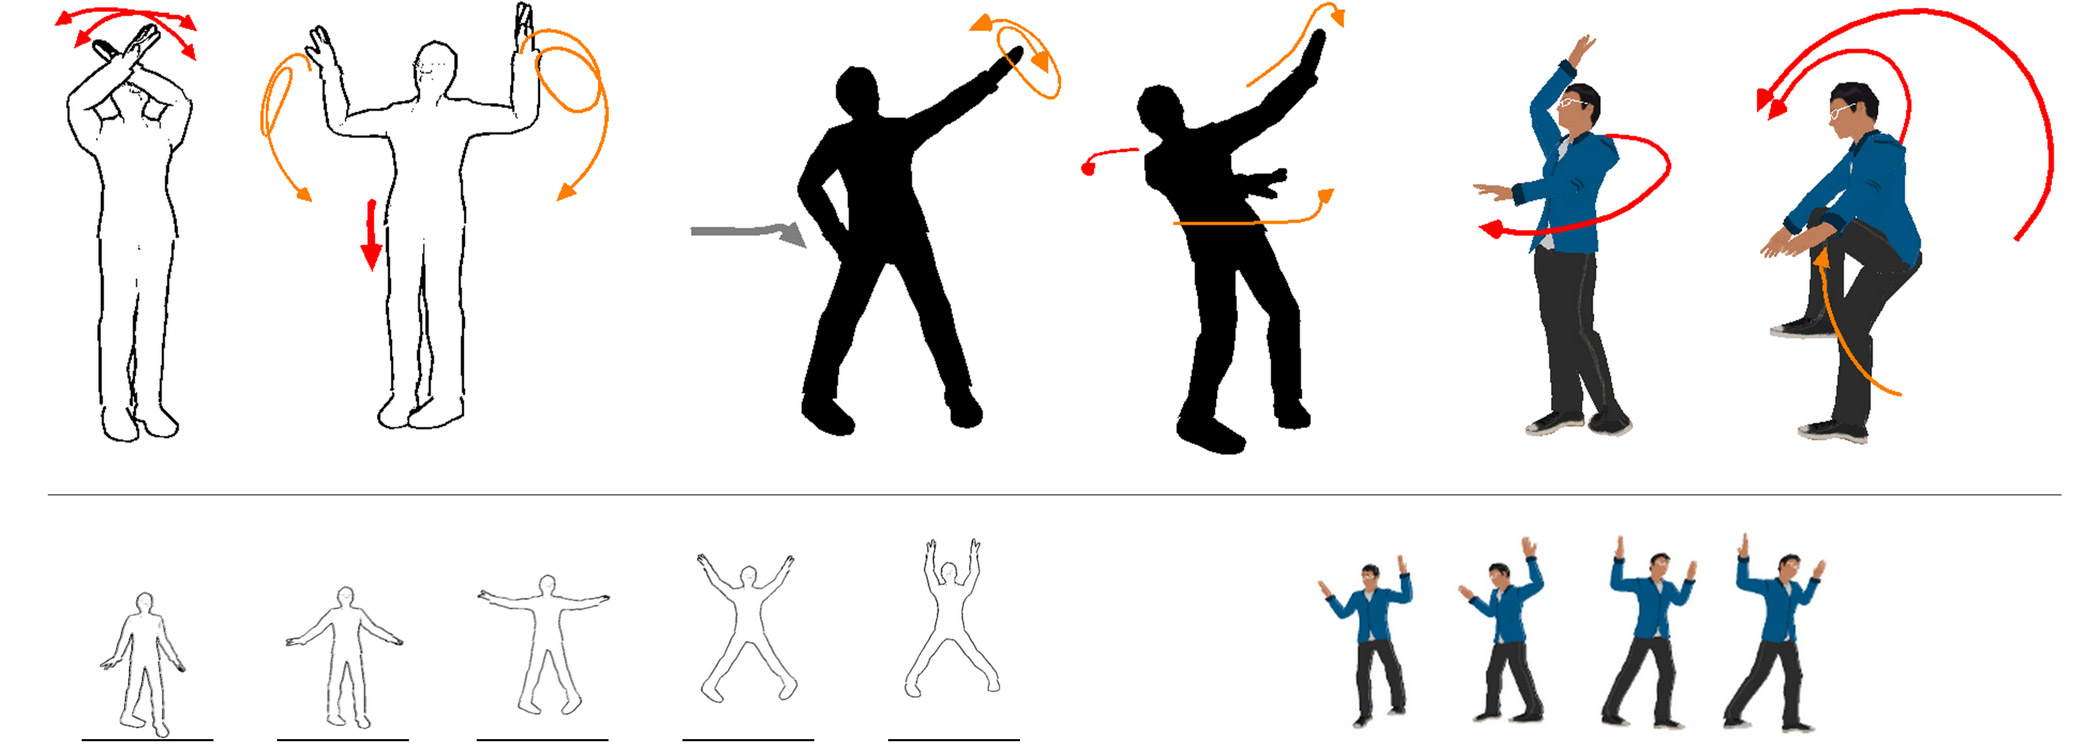
\includegraphics[width=\textwidth]{\mixt/fig/teaser/teaser}
  \caption{MixT generates tutorials that contain static and video information from task demonstrations. Videos are automatically edited and offer different views to highlight the most relevant screen areas for a step. Visualizing mouse movement helps user understand a complex action.}
  \label{fig:mixt_teaser}
\end{figure*}

%!TEX root = ../thesis.tex
\chapter{Introduction}
\label{chapter_introduction}

When attempting to accomplish unfamiliar, complicated tasks, people often look for tutorials to follow instructions. From performing daily tasks such as cooking and operating a machine, using software applications, to physical activities like sports and dance performance, each domain involves specific ``how-to'' knowledge with a certain degree of complexity~\cite{ryle1945knowhow}.
%
Instructions, which describe how a specific goal can be accomplished, are a tool for people to self-learn a task~\cite{Smith03iimanufacturer}. Studies have shown that visual instructions are cognitively favorable by people as they are easier to comprehend and remember than text information~\cite{Harrison:1995uh,mayer1996less,Heiser:2004:IVC:989863.989917}. In history, pictorial instructions have been created from the Middle Age to explain dancing or weapon operations~\cite{mijksenaar1999open}. It was found that the first use of letters in technical drawing for text referral was by Italian polymath Leonardo da Vinci. In 1737, French engineer de B{\'e}lidor~\cite{de1737architecture}'s diagrams were the first to apply arrows to indicate direction of movements (see Figure~\ref{fig:intro_arrows}).
%
From 1760, when the Industrial Revolution introduced mass production, instructions have been seen widely for various products and uses.

\begin{figure*}[h!]
  \centering
  \begin{minipage}{\textwidth}
  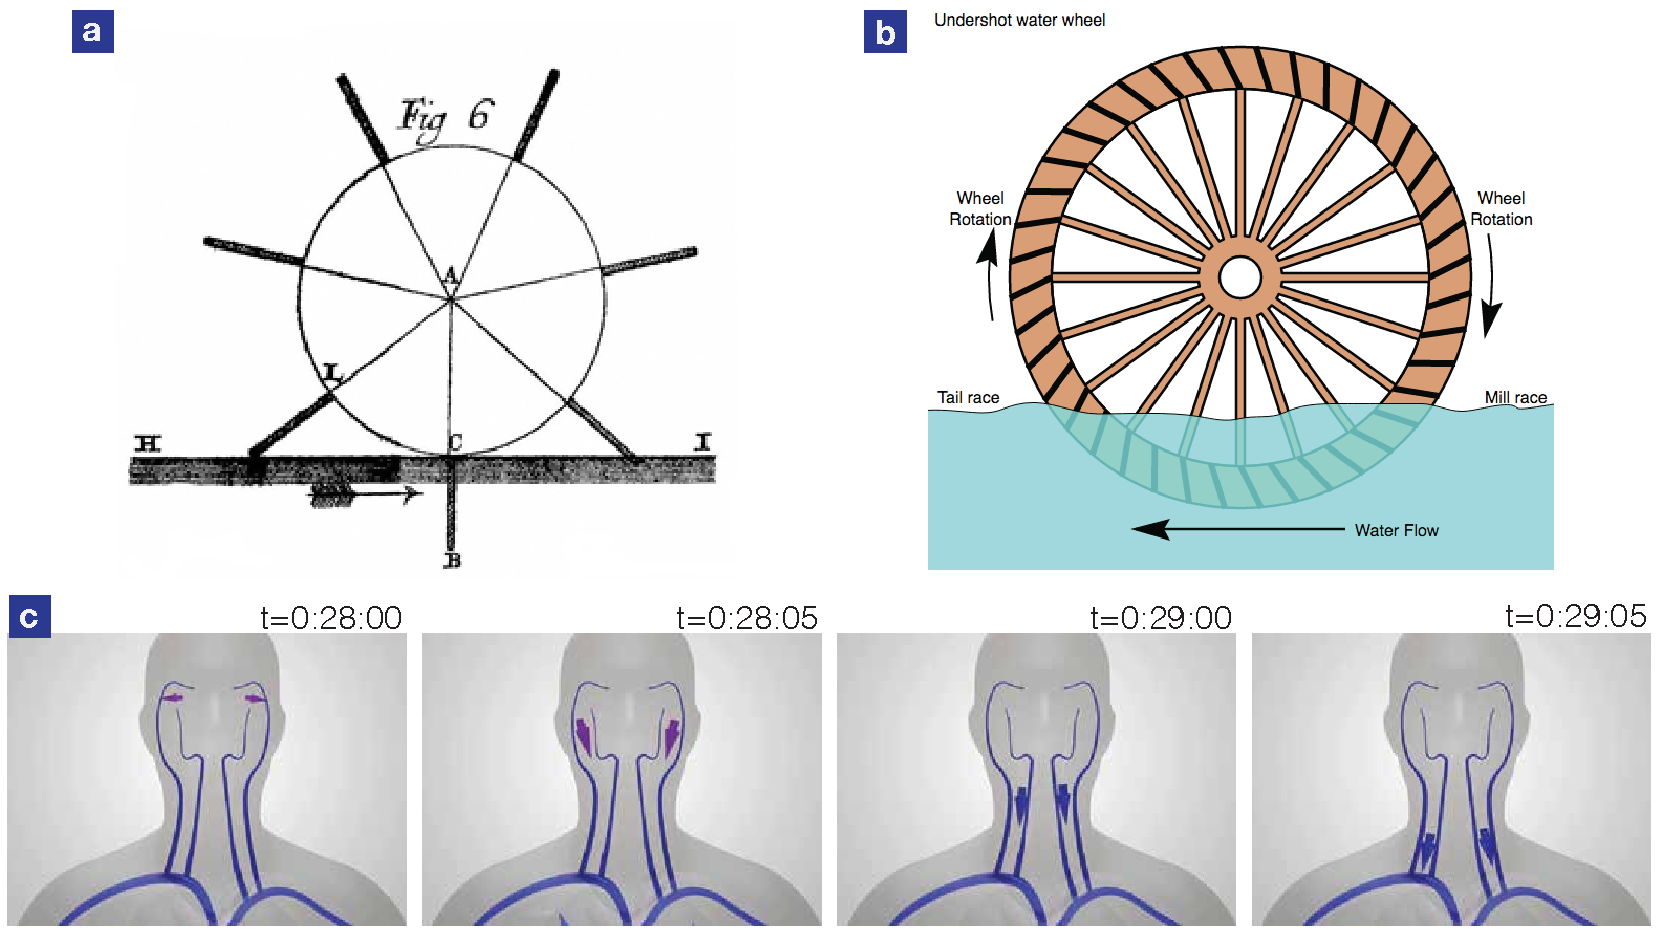
\includegraphics[width=\textwidth]{\intro/fig/arrows/arrows}
  \caption[Uses of motions arrows in visual instructions.]{Uses of motions arrows in visual instructions:
  %
  a) Year 1737: The first use of a motion arrow in an illustration explains the impact of water flow of a water wheel~\cite{de1737architecture},
  % http://www.buw-output-archiv.uni-wuppertal.de/ausgabe1/steinle/index-en.html
  %
  b) Year 2002: Similarly, arrows are used to explain the water flow and rotation of an undershot water wheel\footnote[1]{Original artwork by Daniel M. Short, ``Schematic diagram of an undershot water wheel'', licensed under CC BY-SA 2.5},
  % https://en.wikipedia.org/wiki/File:Undershot_water_wheel_schematic.svg
  %
  c) Year 2014: An animation visualizes the blood flow using motion arrows\footnote[2]{Video by Bioscience Credentials, ``Blood Flow in the Human Body'', \url{https://youtu.be/GwX41xm9esY}, licensed under CC BY 3.0}.
  }
  \label{fig:intro_arrows}
  \end{minipage}
\end{figure*}

Since the late 1990s, the advance in computer technologies has introduced more versatile instructional design. Instructions can now be created via software tools rather than hand drawing; they can include multimedia such as images and videos in several forms; they can be accessed through the Internet, as well as in hard copy.
%  the general purpose computers and the Internet
%
This advancement also enables consumers or end-users to document and share their domain knowledge~\cite{Lafreniere:2012tl}. As of today, popular tutorial sharing sites like Instructables has over 220,000 articles~\cite{InstructablesProjects}, wikiHow provides over 192,000 articles~\cite{wikiHowStatistics}, Food.com serves over 500,000 user-generated recipes with 125,000 photos~\cite{FoodComAbout}, and YouTube hosts over 285 million How-To videos\footnote{YouTube, \url{https://www.youtube.com/}, accessed June 2016}.
%
The variety of topics, content, and presentation styles provides learners more options to understand domain knowledge.
%
However, navigating a tutorial using existing tools remains inefficient for following step-by-step instructions. It can be challenging to observe details from text and images or find specific piece of information in a video through a timeline with conventional video players.
%
On the other hand, producing high-quality instructions that are easy to follow requires authoring expertise and a significant time investment. It involves several stages to design, record, and edit multimedia materials of a task using a variety of creation tools~\cite{Torrey:2007he,Tseng:2014:PVP:2598510.2598540,Muller:2009tw}.\\

The goal of this dissertation is to investigate interactive instructional design and develop computational tools that support the authoring process.
%
To contribute to computational methods of authoring user-generated instructions, two research questions that this work focuses on are:

\begin{itemize}
  \item How can authoring tools support domain experts in efficiently creating effective, high-quality instructions based on video-recorded demonstrations?
  \item How can new tutorial formats help authors better express their intent and help learners understand and follow the author's instructions?
\end{itemize}

This dissertation presents video-based computational approaches that enhance tutorial creation and consumption from author demonstrations.
We encode the current practices from professional authors into automatic algorithms and interactive techniques.
Our goal is to dramatically increase the quality of amateur-produced video instructions, which in turn improves learning for viewers who interactively navigate the content.
%
We will introduce five interactive systems that we develop to address these challenges. These tools cover both software applications (e.g., image manipulation tasks or browser navigation) and physical activities (e.g., Do-It-Yourself projects or dance movements) for recording, editing, and replaying instructional content.

% ---------------------------------------------------------------

\section{Challenges of Creating and Consuming Instructions}

Visual instructions are the dominant form of instructional design~\cite{mijksenaar1999open}. Cognitive load theory of multimedia learning suggests that learners process information using distinct channels, one for visual and the other for verbal formats~\cite{sweller1998cognitive,sweller1988cognitive,paas2003cognitive}. It was found that learners performed better when received a pictorial summary of a scientific system than those who received the full text alone or the full text with the summary~\cite{mayer1996less}.

Among all the multimedia support, videos are a common form to present instructions. We suspect that the great popularity of videos is due to the following reasons:
%
First, consumer devices and software have become affordable for authors to quickly record activities and later share via online platforms at minimum cost.
%
% ** describe the difficulties of making knowledge "explicit", esp. for actions and motions
Second, videos can be an efficient medium to document activities. Transferring know-how concisely and effectively to the audience is challenging. It especially requires efforts when a task involves \emph{tacit knowledge}, which is a kind of knowledge that is difficult to articulate in a written or verbal form~\cite{polanyi1958personal, Klemmer:2006:BMF:1142405.1142429}. Examples of tacit knowledge include dancing, riding a bike, or driving nails with a hammer. Dancers can perform movements fluently with music. If they are asked to focus on the composite pieces, such as the arm and foot actions or rhythm, they might get confused and fail to express the entire movement~\cite{polanyi1958personal}. Very often, recording a video eases the difficulties of describing the entire activities in an explicit form.
%
This leads to another motivation that videos also provide an effective channel to convey ideas with adequate amounts of details. Learners can visually observe the exact actions in a video as if an expert were coaching in person~\cite{Kuznetsov:2010:REA:1868914.1868950}.

However, while videos are easy to produce, they can include a lot of unnecessary footage. Inevitable content such as pauses, mistakes, and long repetitive actions makes it difficult for learners to focus on the most important steps and actions. A lot of authoring effort commonly goes into extracting footage, applying visual effects, and adding subtitles and annotations.
%
In addition, even with a well-edited video, navigating using a conventional video player remains inefficient. Learners with various needs could have a hard time skimming to an interesting moment or perceiving high-level overviews. Alternatively, a pictorial summary or static step-by-step tutorials presented with text and images can effectively guide knowledgeable learners through familiar tasks.

% The goal of this dissertation to develop video-based recording, editing, and playback tools are optimized for creating and consuming instructional demonstrations. I combine the advantage of ubiquitous video recording with the benefits of video and structured tutorial formats. I aim to dramatically increase the quality of amateur-produced video instructions, which in turn improves learning for viewers who interactively navigate the content.

% ----- MixT ----- %

\subsection{New Tutorial Formats}

Both static and video tutorials have strengths, but neither format alone is well suited for all learning needs that learners may have.
%
To combine the benefits, we design a new instructional presentation called \emph{MixT} (mixed-media tutorials) that improves learners' success in following instructions (see Figure~\ref{fig:mixt_intro}).
%
MixT presents step-by-step static instructions and includes in-place video clips for each operation.
%
With MixT, learners can quickly scan forward and backward on a web page to obtain an overview of a task. Embedded videos help them understand continuous, complex manipulation, such as brushing on a canvas and adjusting control points.
%
MixT's playback UI allows learners to interactively control \emph{when} to see images or videos, and \emph{how} to render videos.
%
Video editing techniques are applied to emphasize instructions, including cropping salient screen regions and highlighting interaction.
%
In our within-subject experiment, MixT successfully reduced numbers of errors and attempts made by learners when following image manipulation tasks.
% To demonstrate , MixT captures screencast video and operation events of a software demonstration.

\begin{figure*}[t]
  \centering
  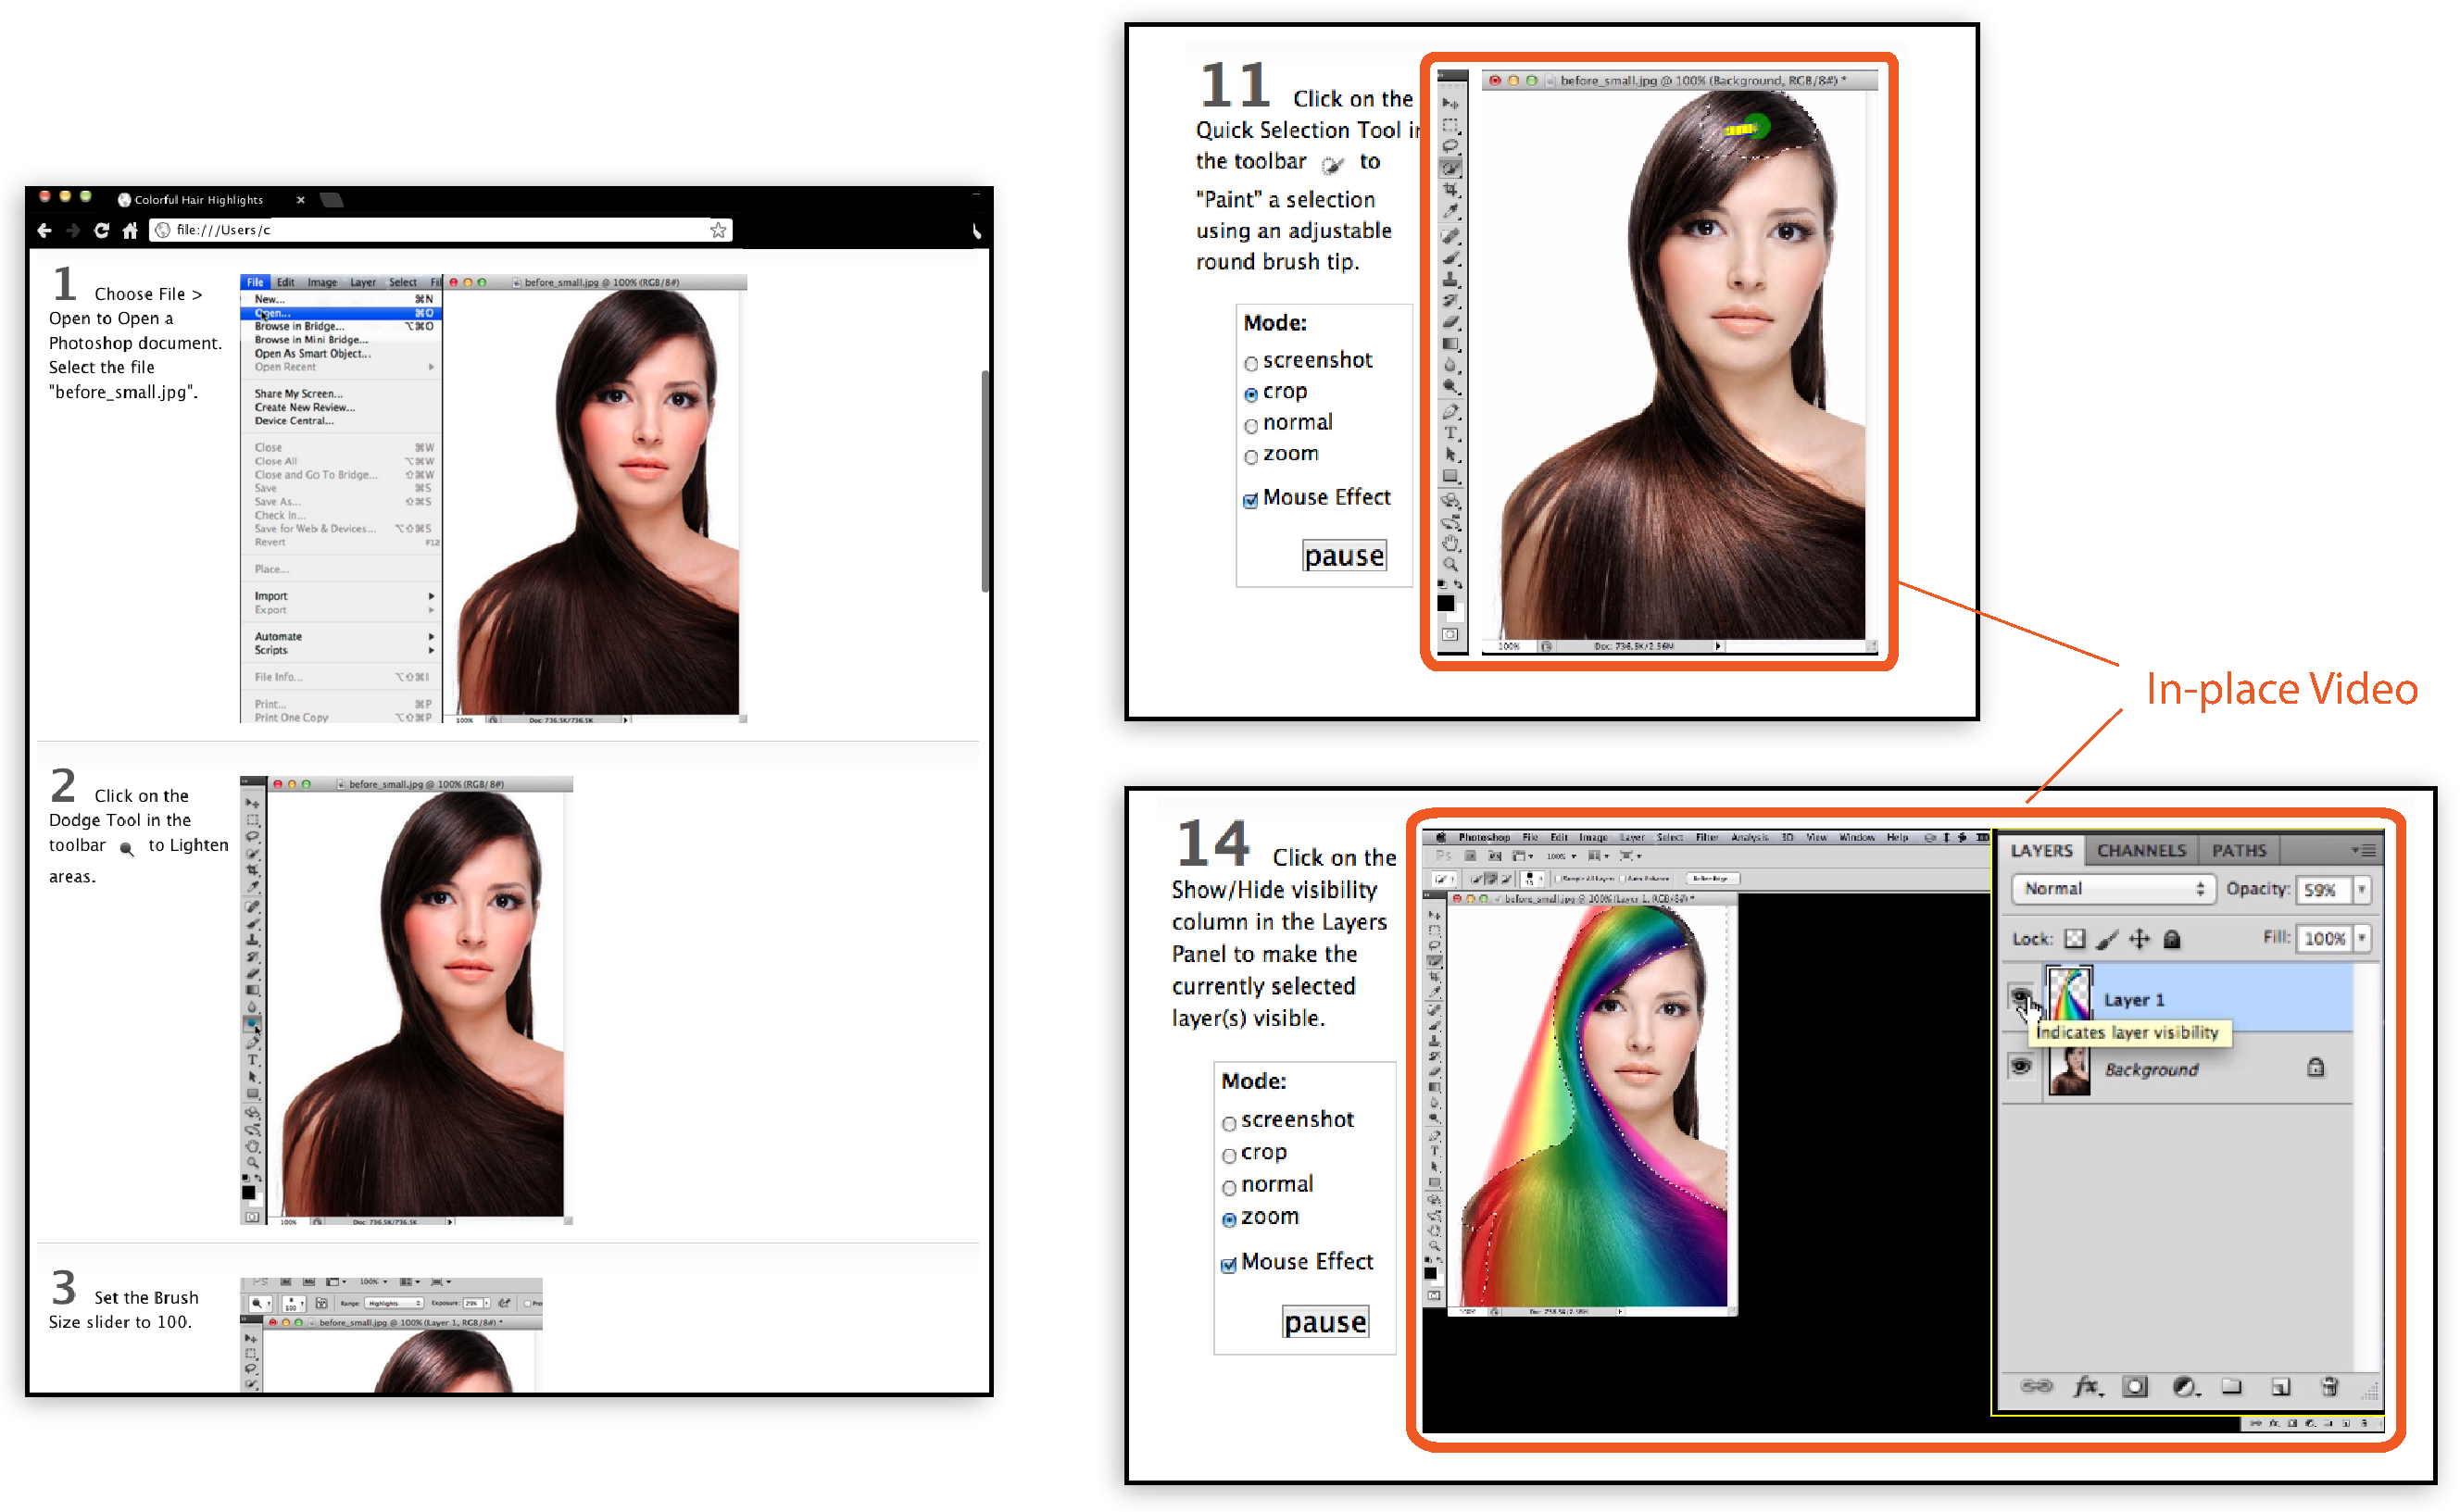
\includegraphics[width=0.8\textwidth]{\intro/fig/mixt_intro}
  \caption{MixT generates step-by-step tutorials (left) that contain static and video information from task demonstrations. Videos are automatically edited and offer different views (right) to highlight the most relevant screen areas for a step. Visualizing mouse movement helps learners understand a complex action.}
  \label{fig:mixt_intro}
\end{figure*}

% ----- DemoWiz ----- %
MixT offers a novel way of navigating instructional content with a combination of static step-by-step and embedded video presentations. If an author wants to narrate over a video recording to illustrate a demo, it can be challenging to pace oneself at the suitable timing without expecting \emph{when} and \emph{what} action is taking while a video is playing.
%
We design \emph{DemoWiz}, a system that augments a screencast video with visualizations (Figure~\ref{fig:demowiz_intro}). By logging the input events of a software demonstration, DemoWiz overlays glyphs to visually guide viewers to the next action along with the time remaining before the action occurs. This enables viewers to anticipate the video content rather than react to it.
%
Our study showed that fewer anticipation errors and narration delays were made with DemoWiz.

\begin{figure*}[t]
\centering
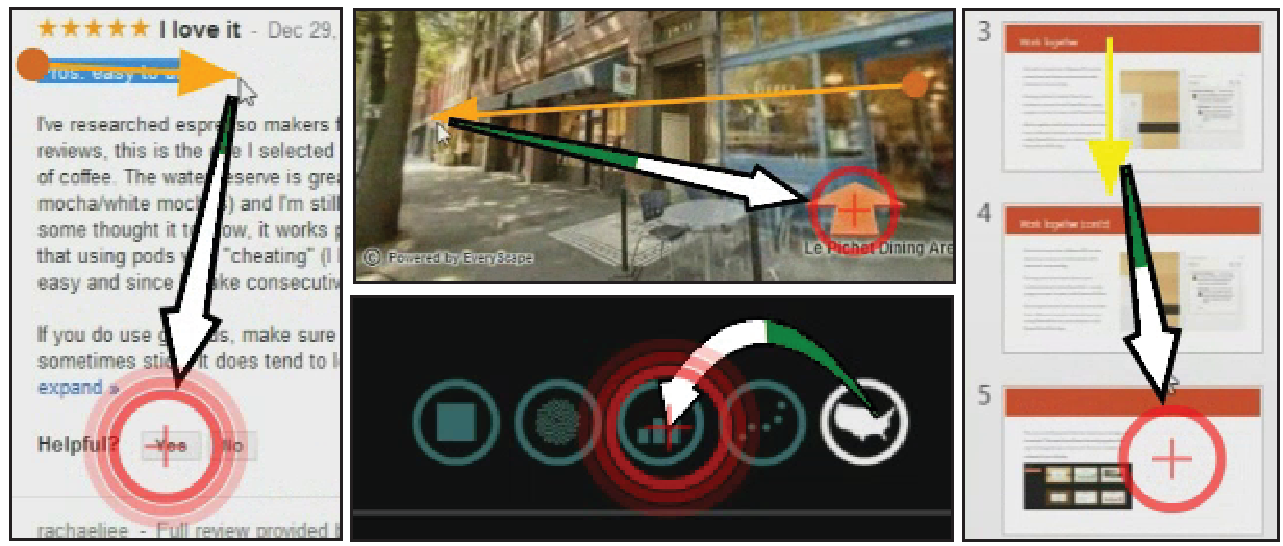
\includegraphics[width=0.7\columnwidth]{\intro/fig/DemoWiz}
\caption{DemoWiz visualizes input events in a screencast video to help viewers anticipate the upcoming event for following a software demonstration.}
\label{fig:demowiz_intro}
\end{figure*}

\subsection{Tutorial Generation from Software Demonstration}

While new tutorial formats are shown to be useful, manually creating instructions can be extremely time- and effort-consuming. In response, we design computational methods to automate the creation process from an author demonstration. MixT and DemoWiz capture screencast video and input device events from a demonstration of a task in a software application. MixT also records application commands for video analysis. Computer vision and visualization techniques are integrated to segment a video into steps, extract salient information, and add visual highlights.
%
In addition, DemoWiz supports an editing phase where authors can adjust the timing of events in a video. Playback speed of recorded actions can be modified or skipped via an editing UI. Our studies showed that our algorithms for step segmentation, event detection, and visualization were effective (\textless8\% error rate in MixT and 0\% in DemoWiz).

\subsection{Interactive Tutorial Authoring from Physical Demonstration}

% ----- DemoCut ----- %

Moving beyond software applications, support for authoring instructions of tasks that take place in the physical world is lacking. Activity recognition remains an open research question, and making authoring decisions during a demonstration can be difficult.
%
To address this problem, we first look into Do it yourself (DIY) project tutorials, which help people learn knowledge and skills to complete a task independently.
%
We developed \emph{DemoCut}, a semi-automatic video editing system that improves the quality of amateur instructional videos for physical tasks (Figure~\ref{fig:democut_intro}). DemoCut asks authors to describe key ``moments'' in a recorded demonstration video using a set of markers. Based on the annotations, our system analyzes the audio and visual activities to automatically organize the video into meaningful segments. Editing decisions are applied to support both \emph{temporal effects} that increase playback speed or skip segments, as well as \emph{visual effects}, such as zooming, subtitles, and visual highlights. A playback interface allows authors to quickly review and edit the automatically generated effects.
%
Our studies showed that video tutorials created by DemoCut in five DIY domains were concise in terms of video length and descriptive instructions with low effect error rates.

\begin{figure*}[t]
  \centering
  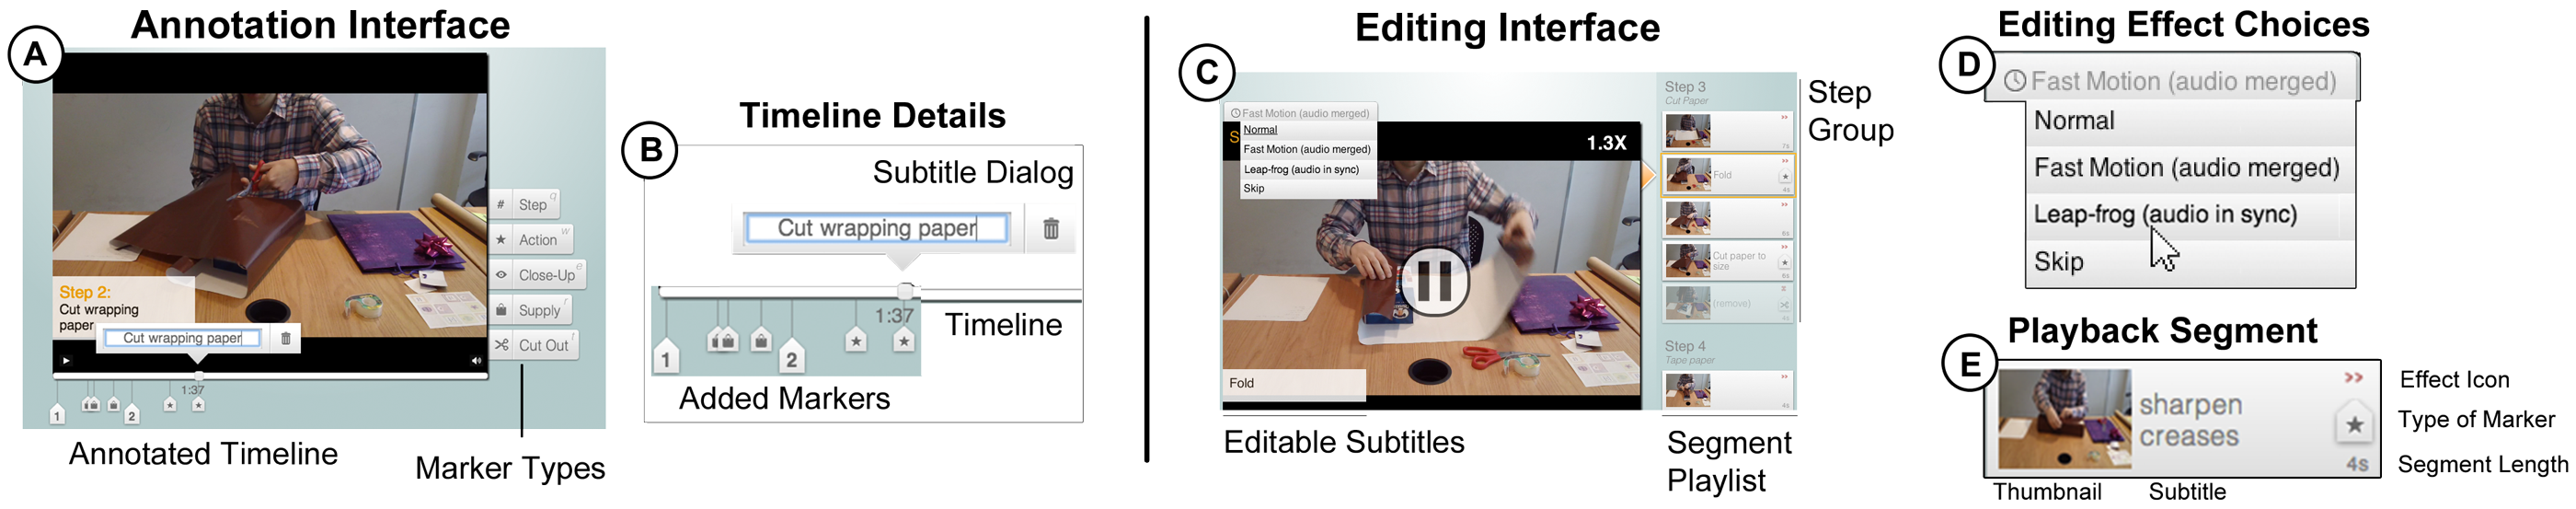
\includegraphics[width=\textwidth]{\intro/fig/DemoCut}
  \caption{DemoCut asks authors to mark key moments in a recorded video of demonstration using a set of marker types. Based on marker information, the system uses audio and video analysis to automatically organize the video into meaningful segments and apply appropriate video editing effects, which can be modified via a playback UI.}
  \label{fig:democut_intro}
\end{figure*}

% ----- Kinectograph ----- %
Through the process of designing DemoCut for automatic DIY video editing, we observed that for tasks that require larger space and more movements, instructors often have to adjust the position and viewing angle of a camcorder. Some authors choose to set up multiple cameras and later select the best shot from video streams, while some invite another person who controls the camcorder during a demonstration.
%
To enable authors to record their demonstration without acquiring additional cameras or cameraman, we design \emph{Kinectograph}, a video recording device with a single camera that automatically tracks and follows specific body parts, e.g., hands, of an instructor in a video (see Figure~\ref{fig:kinectograph_intro}). It utilizes a Kinect depth sensor to track skeletal data and adjusts the camera angle via a 2D pan-tilt gimbal mount. Authors can freely move around in space to demonstrate a task and monitor real-time video preview through a tablet application.

\begin{figure}[!t]
  \centering
  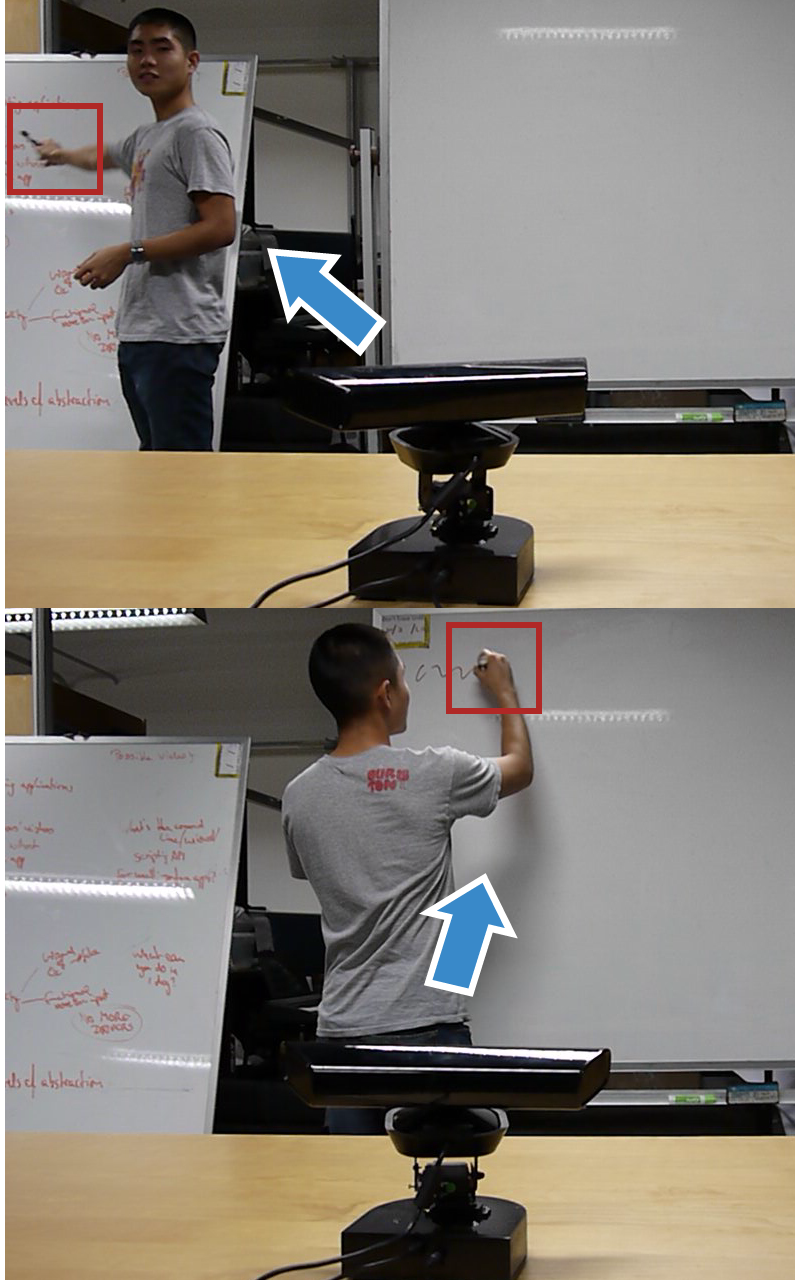
\includegraphics[width=0.65\columnwidth]{\intro/fig/Kinectograph}
  \caption{Composed of a Kinect camera to track author movement and a motorized dock to pan and tilt the camera, Kinectograph allows the author (or their hand) remains centered in the recorded video in real-time.}
\label{fig:kinectograph_intro}
\end{figure}

% ----- DemoDraw ----- %

The successful experiences supporting motion-based recordings motivated me to apply our demonstration-based approach to a domain that is entirely driven by movements. In sports, dance performance, and body gesture interfaces, movement instructions are often conveyed with drawings of the human body annotated with arrows or stroboscopic effects~\cite{cutting_representing_2002}. However, current practices require authors to manually sketch or trace subjects from photographs, which is time-consuming and difficult to make changes once created.
%
We design \emph{DemoDraw}, a system that generates concise illustrations from author demonstration (see Figure~\ref{fig:demodraw_intro}). With DemoDraw, an author records one or more motions by physically demonstrating in front of a Kinect sensor. In a multi-modal Demonstration Interface, DemoDraw segments speech and 3D joint motion into a sequence of motion segments, each characterized by a key pose and salient joint trajectories. Based on this sequence, a series of illustrations is automatically generated using a stylistically rendered 3D avatar annotated with arrows to convey movements. Once a suitable sequence of steps has been created, a Refinement Interface enables fine control of visualization parameters.
%
In a three-part evaluation, our results show 4 to 7-step illustrations can be efficiently created in 5 or 10 minutes on average.

\begin{figure}[t]
  \centering
  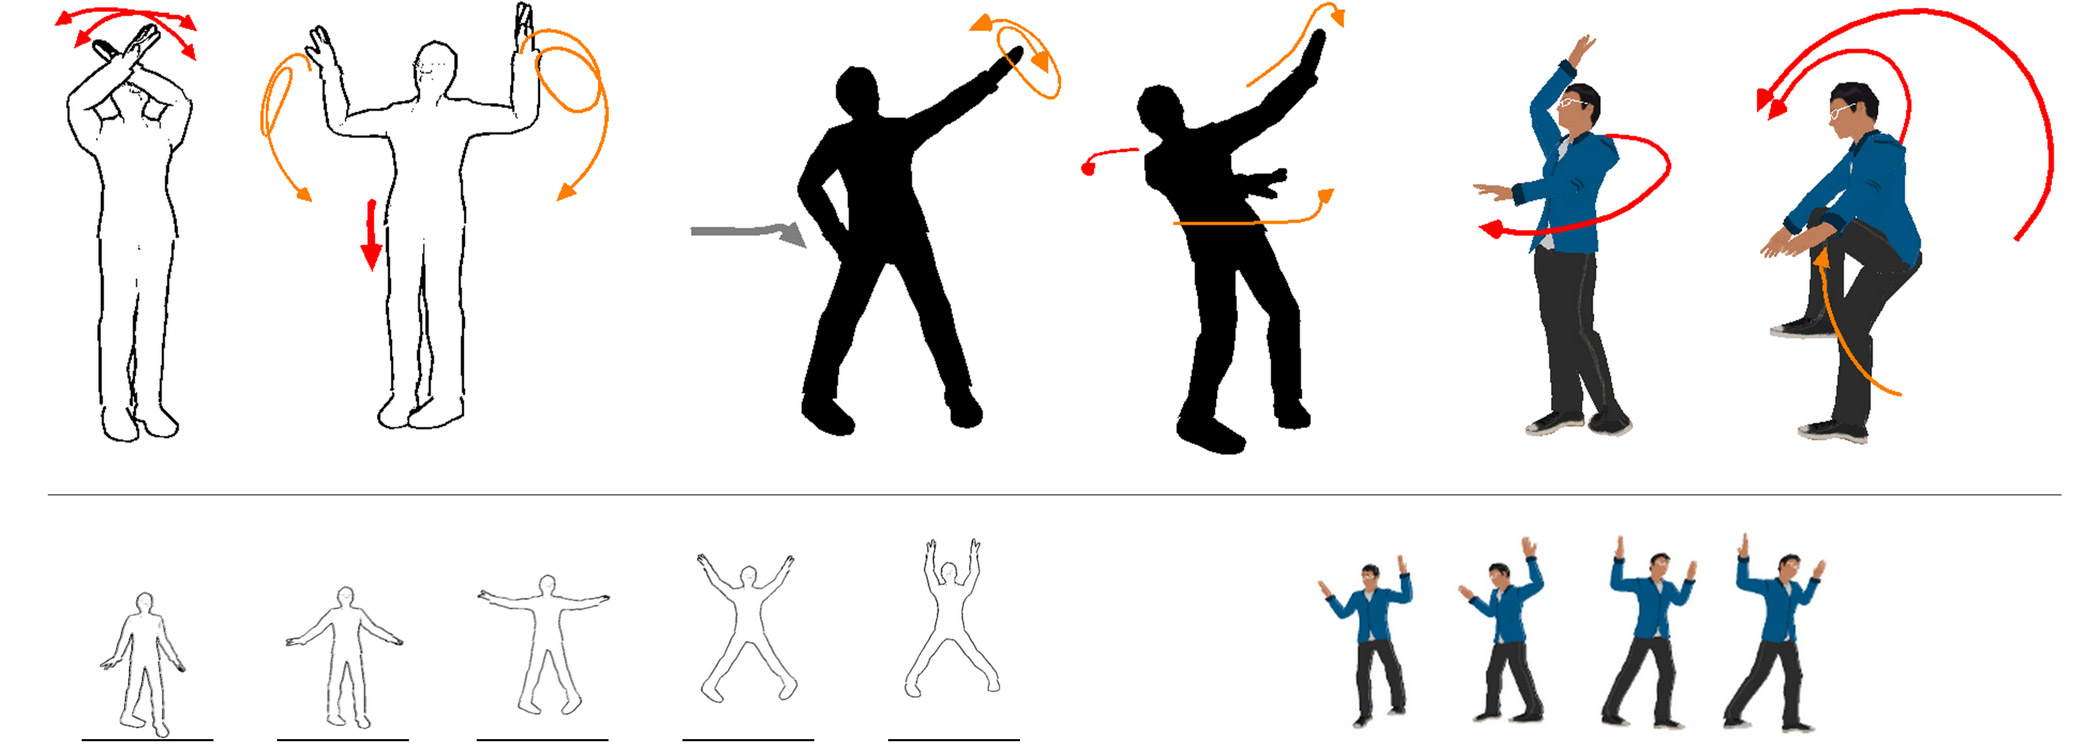
\includegraphics[width=\columnwidth]{\intro/fig/DemoDraw}
  \caption{DemoDraw's multi-modal approach enables authors to capture motion, verify results, and re-perform portions if needed to generate step-by-step motion illustrations.}
  \label{fig:demodraw_intro}
\end{figure}

% ---------------------------------------------------------------

\section{Thesis Contributions}

Overall, our video-based approaches consider key events or moments that are important to a learner. This information can be derived from software event logs or human annotation of physical tasks when automatic recognition remains challenging. Based on the metadata and video streams, we propose automatic methods to generate concise instructions for two task domains, software applications and physical tasks (see Figure~\ref{fig:space}). Our approaches support authors from recording demonstrations to editing and reviewing system-generated instructions. Interactive controls are available in different stages via desktop or multi-modal interfaces.
%
We demonstrate a series of systems that consider production stages of tutorial creation and learning. We present the rationale and technical challenges of these interactive system designs. Each system is evaluated both quantitatively and qualitatively to study the usability in authoring and learning.

\clearpage
The contributions of this dissertation include:

\begin{itemize}
\item New instructional formats that consider the learning needs from several domains, including software applications and physical activities.
\item Multi-modal interaction techniques for novice or amateur authors to create effective instructions by demonstration.
\item Automatic or semi-automatic approaches using video and audio analysis that includes authors in the loop to produce high-quality instructions.
\end{itemize}

\begin{figure}[t!]
  \centering
  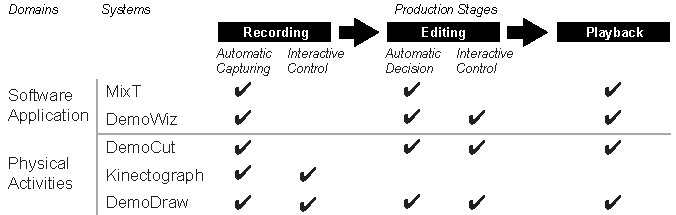
\includegraphics[width=0.9\columnwidth]{\intro/fig/space}
  \caption{A design space of the creation and consumption process for tutorials. It involves three phases of recording, editing, and playback in either software domain or a physical world. This dissertation proposes a series of systems that focus on various aspects in this design space.}
  \label{fig:space}
\end{figure}

% ---------------------------------------------------------------

\section{Overview}

The rest of this dissertation is structured as follows:
%
In Chapter \ref{chapter_background}, we define terminology used in instruction creation and consumption process based on literature. We review studies on why people rely on tutorials in general, how the formats of instructions matter, and the current practices of authoring instructions.
%
In Chapter \ref{chapter_related_work}, we review the literature on research and technologies used in supporting activities of authoring and consuming instructions.

We presented two systems that generate interactive tutorials for software applications.
% MixT
In Chapter \ref{chapter_mixt}, we present our study on how a new tutorial format supports learners in following step-by-step instructions with mixed media, including static text, images, and video clips. We introduce our creation tool called MixT, which automatically generates such new tutorial format from a software demonstration.
% DemoWiz
Chapter \ref{chapter_demowiz} introduces DemoWiz, a system that assists viewers in capturing the timing of input events in a screencast demo video. DemoWiz supports recording, editing, and reviewing stages in a production process with an authoring and playback UI.

Then, we introduced three systems designed for real-world tasks that involve physical demonstrations.
% DemoCut
In Chapter \ref{chapter_democut}, we present a semi-automatic tool for DIY video editing. Our system, called DemoCut, provides two authoring interfaces, annotation and editing, that enable authors to mark a demo video and review and modify the automatically edited results. The design is based on an fundamental understanding of DIY activities.
% Kinectograph
In Chapter \ref{chapter_kinectograph}, we focus on a recording device that automatically follows a demonstrator for filming instructional videos. The Kinectograph system tracks an author's position and body parts and provides an authoring interface for real-time camera control.
% DemoDraw
Finally, in Chapter \ref{chapter_demodraw}, we introduce a multi-modal approach for authors to generate motion illustrations by physically demonstrating the movements. DemoDraw is a system that segments speech and 3D joint motion into a sequence of motion segments and renders effective illustrations. Two authoring interfaces enable authors to navigate, re-perform, and edit visualization parameters.

% Conclusion
Throughout this dissertation, we discuss how our video-based approaches increase the quality of amateur-produced video instructions. Chapter \ref{chapter_conclusion} concludes our work on tutorial creation and consumption in both software and physical instructions. New directions for future research on interactive tutorials are proposed.

% ---------------------------------------------------------------

\section {Prior Publications}

This dissertation is based on papers published in previous ACM conference proceedings: the MixT system was published at UIST 2012~\cite{Chi:2012:MAG:2380116.2380130}, DemoWiz at CHI 2014~\cite{Chi:2014:DRS:2556288.2557254}, DemoCut at UIST 2013~\cite{Chi:2013:DGC:2501988.2502052}, and Kinectograph at CHI 2013~\cite{Cheng:2013:BCC:2468356.2468568}; DemoDraw will be published at UIST 2016~\cite{Chi:2016:DemoDraw}.

While I am primary author on all publications and led the described projects, this research could not have been completed without my advisor Bj\"orn Hartmann and my collaborators that I have been fortunately to work with. Specifically, Dr. Mira Dontcheva and Dr. Wilmot Li at Adobe Research provided valuable guidance on three projects (MixT, DemoCut, and DemoDraw); Dr. Steven M. Drucker and Dr. Bongshin Lee at Microsoft Research guided the DemoWiz project with their expertise on visualization; Professor Daniel Vogel at University of Waterloo greatly contributed to the DemoDraw project. A group of MS and undergrad students at UC Berkeley and Adobe contributed to implementation, design, and user study in the projects, including Sally Ahn and Amanda Ren in MixT, Joyce Liu and Jason Linder in DemoCut, and Derrick Cheng and Taeil Kwak in Kinectograph.

% We are all natural performers. Humans are proficient at demonstrating how to perform a task in action. However, articulating knowledge into a written or structured form can be extremely difficult. From dancing, repairing a machine, to operating software applications, it remains a challenge how everyday activities can be efficiently captured for a remote learner to understand.

%!TEX root = ../thesis.tex

\chapter{Related Work}
\label{chapter_related_work}

While existing practices require tutorial authors to create instructions manually, HCI and Computer Graphics communities have introduced novel technologies for authoring tutorials, including automatic generation methods and interactive editing tools.
%
In this chapter, I survey state-of-the-art techniques for generating instructions for both software applications (Section \ref{related_software}) and physical tasks (Section \ref{related_physical}).
%
Furthermore, existing instructions are mainly offered in the forms of conventional media, such as static tutorials (print-outs or web) or videos. With software systems, \keyword{interactive tutorials} have been introduced for learners to interactively review instructional content. I will discuss various forms of such kind of instructions by prior research, which leads to a discussion on the remaining gaps in tool support for creating and navigating instructional content.

% -------------------------------------------

\section{Instructions for Software Applications}
\label{related_software}

\subsection{Workflow Capturing and Tutorials}

Revealing operation history has shown to be effective in presenting software instructions. Operational events can range from low-level, application agnostic input device events (e.g., mouse actions, cursor movements, or keyboard strokes) to higher level, application-dependent information (e.g., menu selections or UI component changes).
%
Researchers have investigated automatic approaches that capture and visualize these types of events. Nakamura and Igarashi~\cite{Nakamura:2008:ASV:1449715.1449721} proposed a capturing and rendering system independent to GUI applications. Their system logs mouse events of a software demonstration process, including mouse moving, dragging, and clicking. Operations are rendered as markers and arrows on screenshot images to present the linear event history (see Figure~\ref{fig:related_events} top).
%
Grabler \ea{}'s approach~\cite{Grabler:2009jj} further analyzes the application context, including facial features and outdoor scenes, and annotates software screenshots with arrows, bounding boxes, and call-outs (see Figure~\ref{fig:related_events} bottom). In addition to annotated images, their system generates textual description from templates, such as \iquote{Select the \textbf{path tool} from the \textbf{toolbar} to \textbf{create and edit paths}.} The generated text and rendered images of operations are presented as a step-by-step tutorial, which is currently available as a Photoshop plug-in\footnote{Adobe labs. Tutorial Builder. \url{http://labs.adobe.com/technologies/tutorialbuilder/}}.

Demonstration-based approaches for generating instructions have been also applied to applications that involve more complicated manipulations or gestures, including 3D mesh construction~\cite{Denning:2011fy} and mobile apps~\cite{Wang:2014:EAC:2556288.2557407}.
%
Beyond logging events from recording a user demonstration, researchers have shown that workflows and software content can be captured automatically using application logs \cite{Grossman:2010jz,Grabler:2009jj,Pongnumkul:2011ju} or computer vision from analyzing desktop regions~\cite{Yeh:2009dh,Chang:2011vd} and existing screencast videos~\cite{Banovic:2012kd}.

\begin{figure*}[t!]
  \centering
  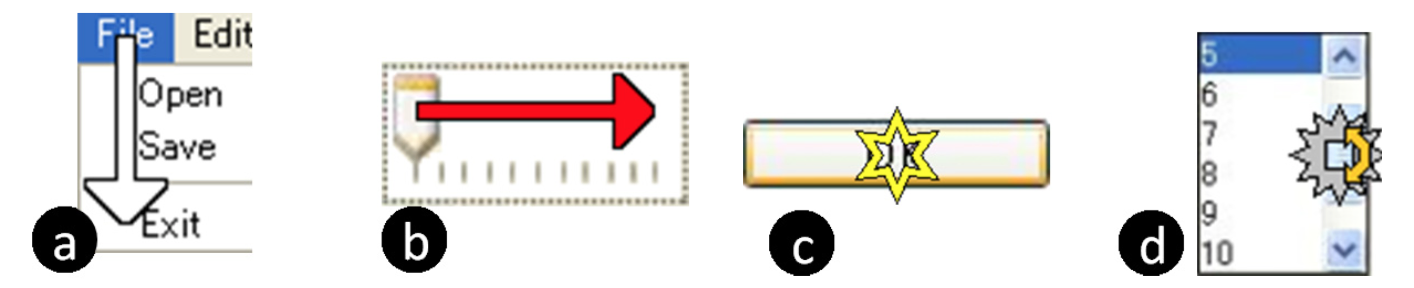
\includegraphics[width=0.6\textwidth]{\background/fig/software_viz/Nakamura_and_Igarashi}
  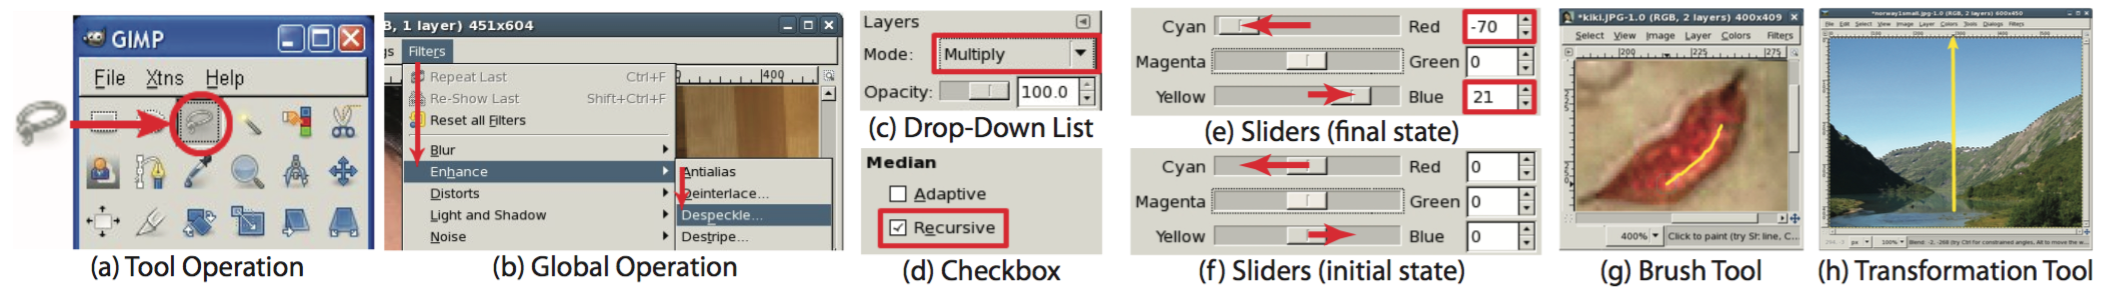
\includegraphics[width=\textwidth]{\background/fig/software_viz/Grabler}
  \caption{Example screenshots that visualize mouse operations are automatically rendered, including (top) mouse move, drag, click, and wheel (a-d) by Nakamura and Igarashi~\cite{Nakamura:2008:ASV:1449715.1449721} and (bottom) application-specific operations (a-b), parameters (c-f), and manipulations (g-h) by Grabler \ea{}~\cite{Grabler:2009jj}.}
  \label{fig:related_events}
\end{figure*}

To compare operation effects and workflows, other effective visualization approaches include showing a list of ``before'' and ``after'' thumbnails, video clips, and event timeline \cite{Grossman:2010jz} and creating a union graph of operations \cite{Kong:2012:DTR:2207676.2208549} (see Figure~\ref{fig:related_comparison}).

\begin{figure*}[t!]
  \centering
  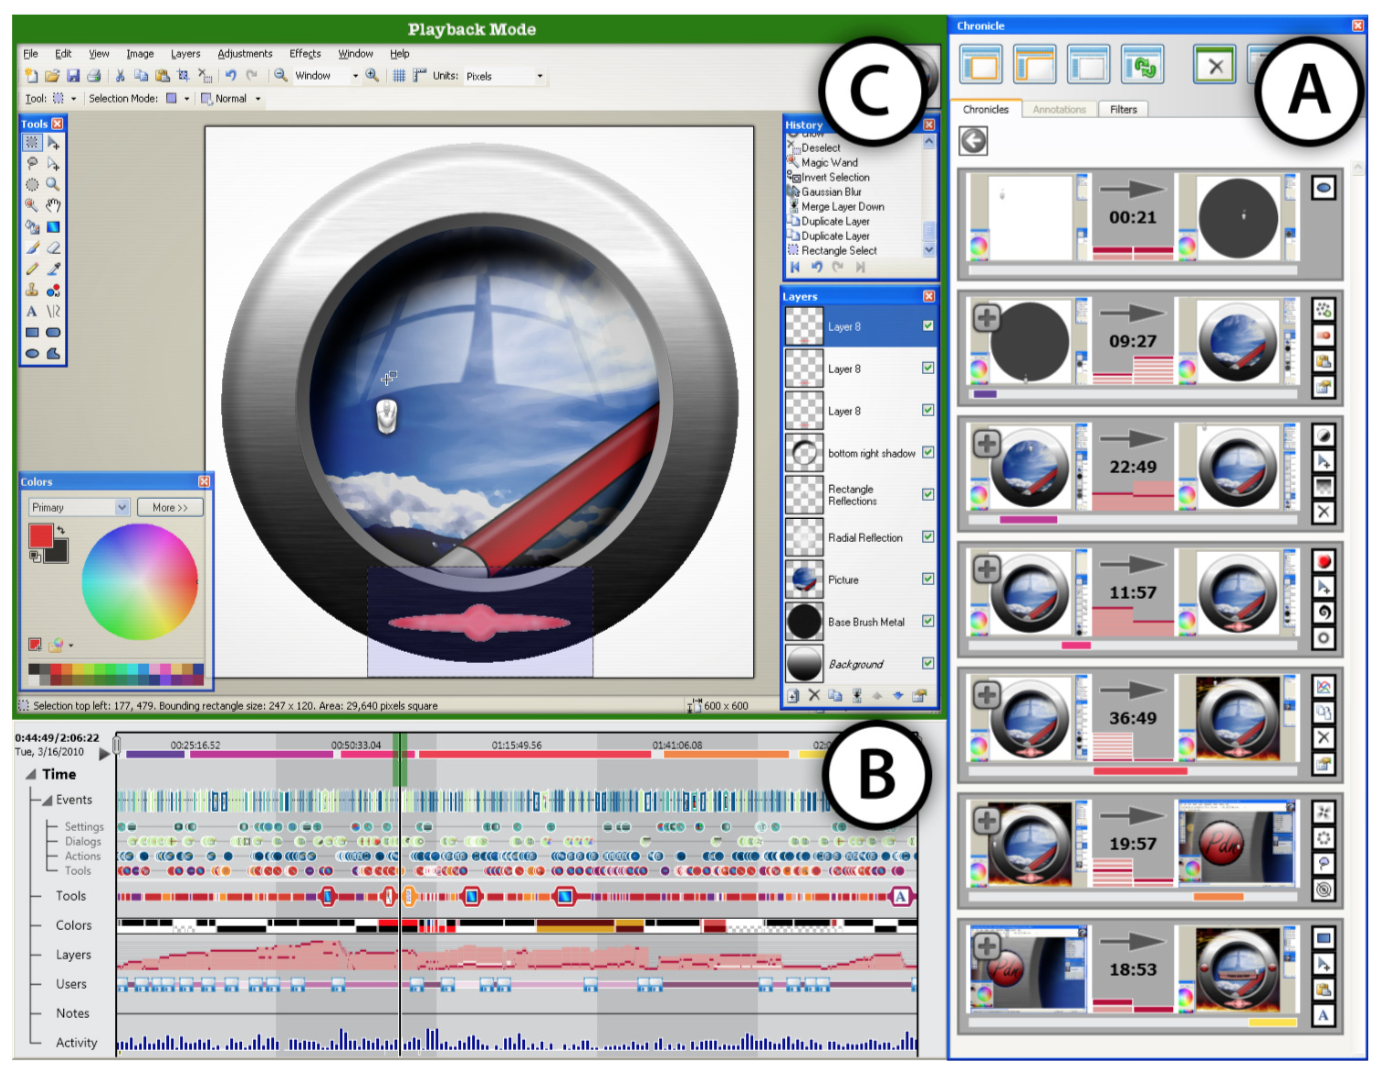
\includegraphics[width=0.4\textwidth]{\background/fig/software_viz/Grossman}
  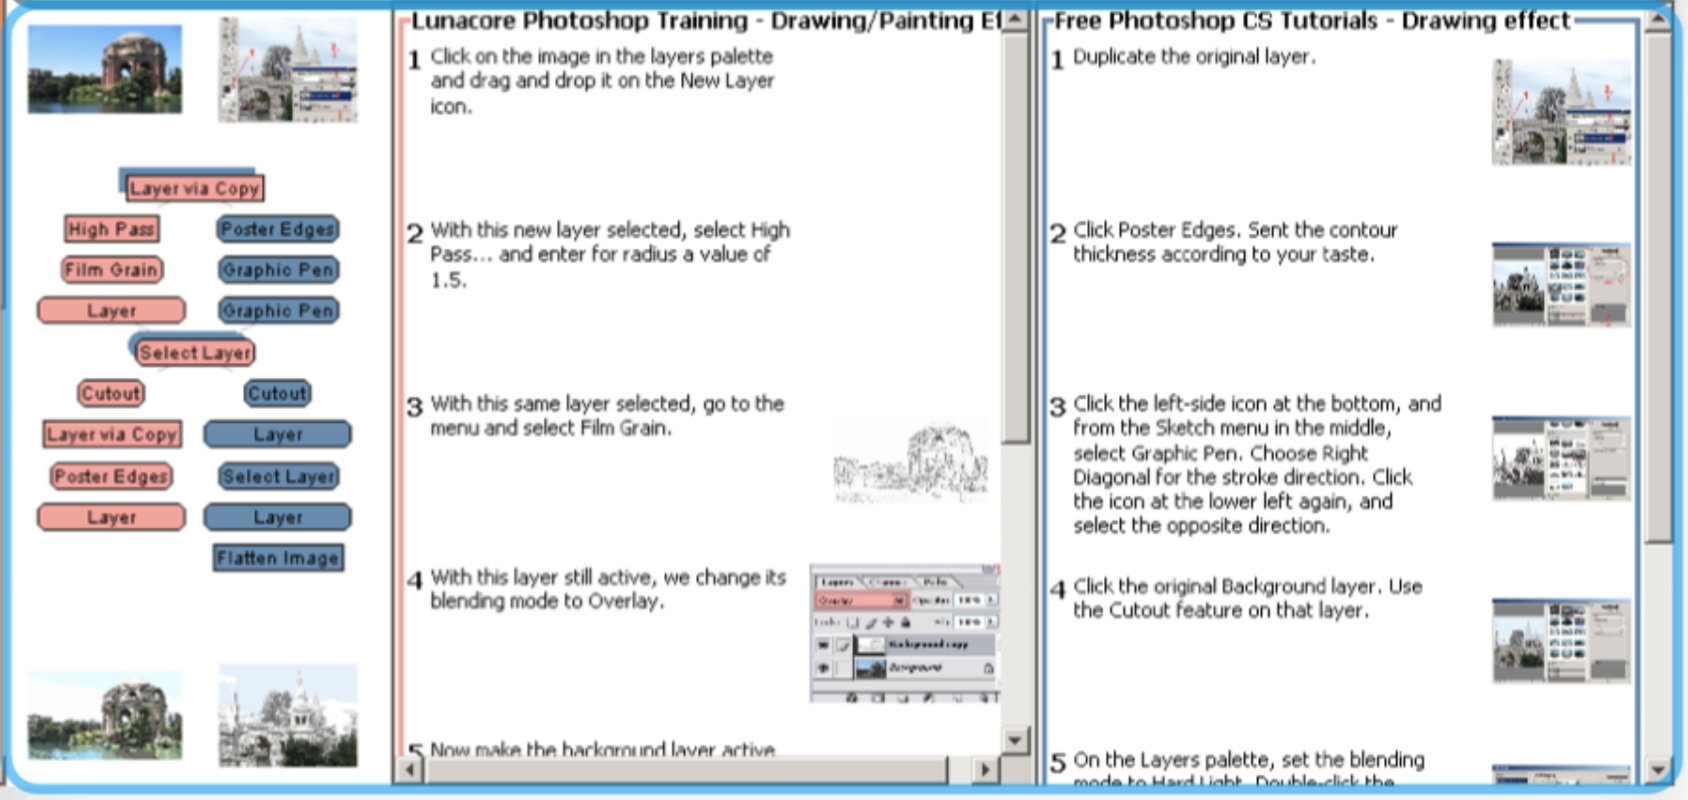
\includegraphics[width=0.55\textwidth]{\background/fig/software_viz/Kong}
  \caption{Instructional systems that help learners compare effects and similar tutorials using: (left) before and after images (a) and event timeline (b) by Grossman \ea{}~\cite{Grossman:2010jz} and (right) operation union graph by Kong \ea{}~\cite{Kong:2012:DTR:2207676.2208549}.}
  \label{fig:related_comparison}
\end{figure*}

% -------------------

\subsection{In-Application Support}

The above systems introduce innovative ways of providing informative screenshots or representations for learners to review workflows. However, reviewing these materials is often separated from operating a software application. Learners might have to switch between context of interacting an application and reading instructions, which could introduce a gap of evaluation (\iquote{Am I doing this right as the instructions explain?}) and a gap of execution (\iquote{How do I perform the action that the instructions describe?}).
%
Researchers have proposed another approach to provide ``in-application'' assistance, often in real-time, in a specific application context.

Studies have shown that visualizing input events in real-time during operations can provide better learnability of applications \cite{Dixon:2010fb}.
%
Commercial tools such as Mouseposé\footnote{Mouseposé \url{http://www.boinx.com/mousepose}} and ScreenFlow\footnote{ScreenFlow \url{http://www.telestream.net/screenflow}} visualize mouse and keyboard events with special effects, such as drawing a circle around a mouse cursor (see Figure~\ref{fig:related_realtime} top).
%
Dixon \ea{} proposed techniques to provide pixel-based enhancements in real-time, such as highlighting nearest regions of interest or applying afterglows based on the current user operations \cite{Dixon:2010fb,Dixon:2011:CHP:1978942.1979086} (see Figure~\ref{fig:related_realtime} bottom).

\begin{figure*}[t!]
  \centering
  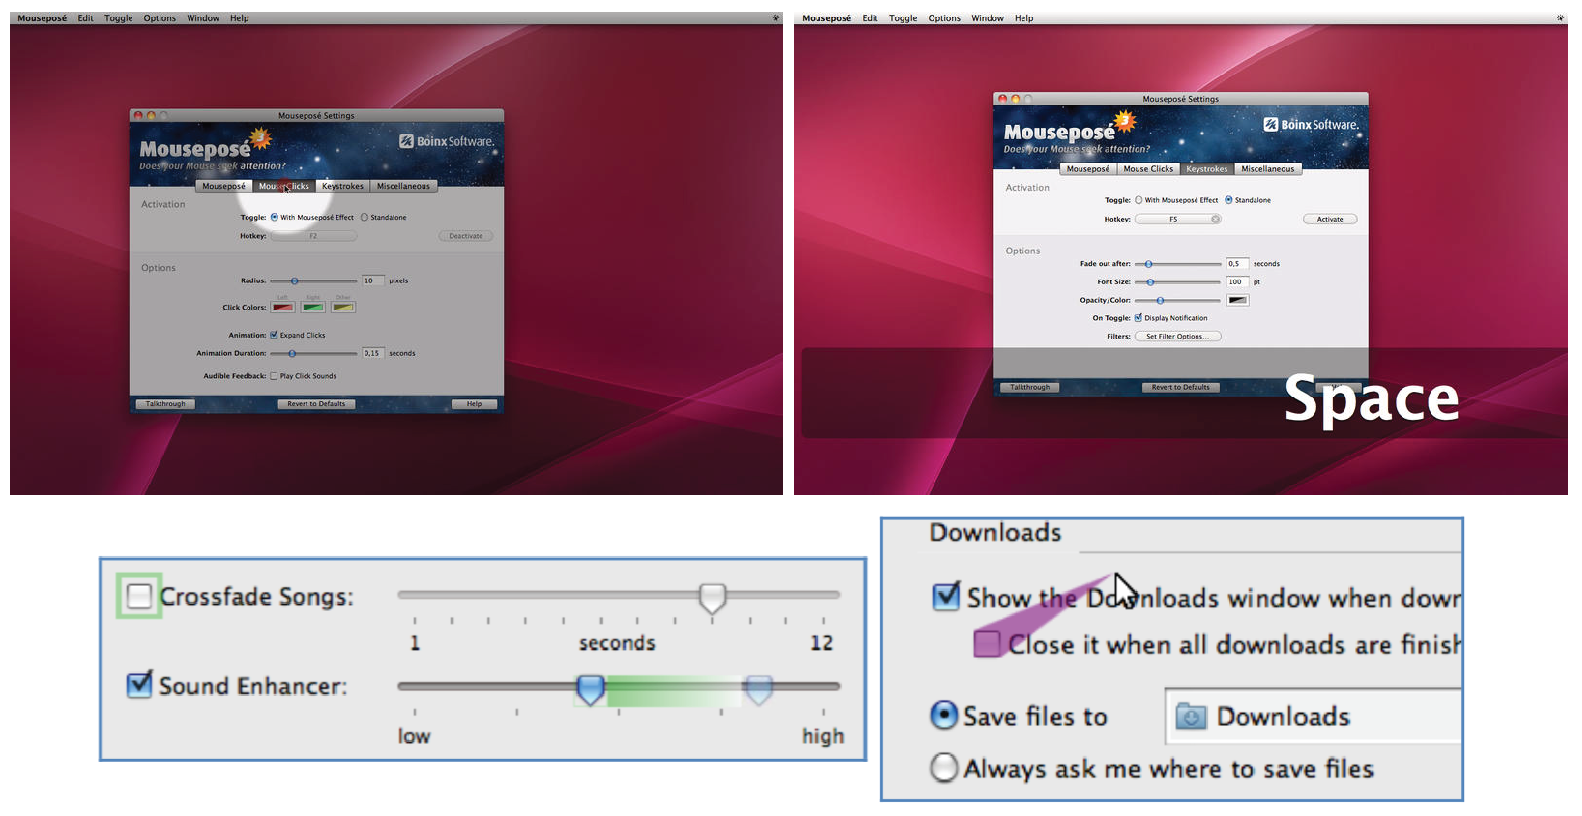
\includegraphics[width=0.7\textwidth]{\background/fig/realtime/realtime}
  \caption{Real-time visual enhancements on GUI applications: (top) Mouseposé highlights mouse cursors or text input; (bottom) Prefab creates target-aware or afterglow effects during user operating~\cite{Dixon:2010fb}.}
  \label{fig:related_realtime}
\end{figure*}

Real-time visual effects help users focus on the region of interest in a GUI application, but to support learners comprehend the application functionalities, there has been a considerable amount of research devoted to offering interactive helps.
%
Video snippets can be embedded in application tooltips~\cite{Grossman:2010wr}, which were shown to be seven times more effective than conventional tooltips for completing unfamiliar tasks.
%
Interactive, step-by-step instructions can be integrated in several forms:
%
To help user identify the correct UI components, tutorials can be shown via translucent colored ``stencils,'' which visually direct user's attention directly in an application~\cite{Kelleher:2005:STD:1054972.1055047}.
%
By tracking user's current operations, tutorials can be embedded in an application to provide instant feedback such as a check-mark or a percentage match~\cite{Fernquist:2011:SRE:2047196.2047245}, automatically replayed to provide the corresponding video instructions~\cite{Pongnumkul:2011ju}, or be shown as ambient help~\cite{Matejka:2011:AH:1978942.1979349}.
%
Instructions can be captured from demonstration as ``scripts'' for step-by-step navigation~\cite{Bergman:2005:DocWizards}. Having more user controls~\cite{Lieberman:2014:SML:2557500.2557543} or being enhanced with game elements~\cite{Li:2014:CGM:2556288.2556954, Dontcheva:2014:CCL:2556288.2557217} can further engage users in learning.

Last but not least, as tutorials are built for a broader community with a set of authors and learners, content can be dynamically updated within a community based on user contribution~\cite{Lafreniere:2013ff,Matejka:2009:CCR:1622176.1622214, Bunt:2014:TPI:2556288.2557118}.

interactive-visualization~\cite{Kwon:2016:CEO:2858036.2858101}
the paper that cited DemoWiz~\cite{Nguyen:2015:MST:2702123.2702209}

% These projects show how effective instructional representations can assist learners in learning or executing tasks. Our goal is to further study new formats that incorporate advantages of several formats of multimedia, including images, text, and videos, and in turn enhancing the learning experience for a variety of tasks.

% * define ``automatic''
% Note: MixT tutorials are automatically rendered from manual demonstration, not automatically generated.

% To provide real-time assistance, it is important to recognize the user activities during a task performance. Several domains have been widely studied, including software operations, scene recognition, and object tracking in a physical world.

% -------------------------------------------

\section{Instructions for Physical Activities}
\label{related_physical}

The above approach of tracking user behavior to automate tutorial authoring opens the door to interactive tutorials that can respond to user progress. However, tracking user behavior in the physical world, rather than in software, remains a challenge.

\subsection{Generating Instructions for Real-World Tasks}
Researchers have investigated tools for automatically generating visual instructions for physical tasks~\cite{feiner:1985:AEA:1299975.1300548,Seligmann:1991:AGI:127719.122732}. Workflows can be captured and created for furniture \cite{agrawala2003designing} or block assembly tasks \cite{Gupta:2012ku}.
%
If video content is difficult to be extracted, crowdsourcing algorithms have been introduced to structure step-by-step videos by online workers~\cite{Kim:2014:CSI:2611222.2556986}.
%
% New devices to support authors capturing multi-media materials, such as a turntable~\cite{Tseng:2015:SPT:2771839.2771869}
% documentation \cite{Tseng:2016:makeology}

\subsection{Interactive Guidance}
To provide responsive instructions, a computer system needs to understand user operations in real-time. Ideally, activities should be automatically tracked without human labeling.
%
Computer vision techniques can track specific physical targets, including hands \cite{Ranjan:2008}, user movements \cite{Wilson:2012fb}, fast-moving objects (e.g., a Ping-Pong ball) \cite{Okumura:2011tr}, or regions in pre-defined spaces \cite{Ranjan:2007}.
%
These methods usually require an expert defining heuristics of space regions or movement classifications ahead of time for the tracking program.
%
Thanks to the advance of technology, camera sensors such as Kinect have become widely available to track activities for block assembly~\cite{Gupta:2012ku} and dance~\cite{Anderson:2013:YEM:2501988.2502045}.

Real-time guidance is often shown via an external display, placed next to the working area~\cite{Gupta:2012ku}. To better blend the information into activities, Knibbe~\ea{} design a display-embedded table as a physical workspace that monitors, records, and assists users~\cite{Knibbe:2015:SMI:2817721.2817741}.
%
Alternatively, information can be overlaid on top of the work area using augmented reality, usually through a head-mounted display. Such systems can provide visual highlights for machine maintenance~\cite{Henderson:2011ff}, or interactive remote tutoring for repair tasks~\cite{Gurevich:2012ko}.
%
Another method is to overlay guidance on an augmented mirror for tasks such as dance movements~\cite{Anderson:2013:YEM:2501988.2502045}.

for Frisbee players~\cite{Solomon:2014:UTI:2540930.2540965}

% Lovell and Buechley use electrical sensing with conductive thread for a sewing tutorial~\cite{Lovell:2010tl}.

% I aim to propose a new approach that gives users flexibility in a home environment, and provides interactive control. If activity recognition is not possible, my approach includes users in the loop to annotate high-level information in order to create high-quality results.

% -------------------------------------------

\section{Working with Videos}

\tofix{intro here}

\subsection{Capture}
Several research and commercial systems guide users at capture time to yield higher-quality videos. Such systems often employ templates to help users capture sequences of distinct shots (e.g., Snapguide\footnote{\url{http://snapguide.com/}}) or suggest framing of the subject or camera view as in NudgeCam~\cite{Carter:2010}. Computer vision algorithms, like face tracking, can be used to offer real-time feedback during such directed actions~\cite{Davis:2003cu,Heer:2004ba,Carter:2010}. Instead of relying on templates, shot suggestions can also be bootstrapped through user dialogs~\cite{Adams:2005}.

\subsection{Annotation}
Researchers have investigated how to provide interactions that enable efficient, fluid annotation of video data, from the early EVA system~\cite{Mackay:1989} to more recent interfaces like VideoTater that leverage pen input~\cite{Diakopoulos:2006vt}.

\subsection{Editing}
Frame-based editing of video is very time-intensive, as it forces users to operate at a very low level of detail. Editors can leverage metadata, such as transcripts~\cite{Berthouzoz:2012,Pavel:2014:VDB:2642918.2647400} and shot boundaries~\cite{Casares:2002dx}, to give users higher-level editing operations at the shot level rather than the frame level.
In specific video domains like interview videos, transcripts can help users place cuts and transitions~\cite{Berthouzoz:2012}.
%
Computer vision techniques can automate certain effects, such as creating cinemagraphs~\cite{Bai:2012, Joshi:2012}, automatically-edited lecture videos~\cite{Heck:2007}, zoomable tapestries~\cite{Barnes:2010} and synopses~\cite{Pritch:2009vl}, or stabilizing shaky amateur videos~\cite{Liu:2011}. When analyzing video is a matter of subjective taste, identifying salient frames can also be outsourced to crowd workers~\cite{Bernstein:2011uj}.

live authoring through compositing and editing of streaming video~\cite{Freeman:2014:LLA:2611105.2557304}

\subsection{Navigating}
Videos can be navigated at the content level beyond log events, such as visualizing subject movements in a storyboard design \cite{goldman2006schematic} and enabling direct manipulation of a target in 2D \cite{Dragicevic:2008:VBD:1357054.1357096,Goldman:2008:VOA:1449715.1449719,Karrer:2008:DDM:1357054.1357097} or 3D \cite{Nguyen:2013:DMV:2470654.2466150}. These techniques help viewers understand content flow and playback videos, and have been applied to screencast videos \cite{Denoue:2013:RDM:2451176.2451190}. It is also possible to automate video control based on user actions for scenarios such as operating software applications~\cite{Pongnumkul:2011ju} and block assembling tasks \cite{Gupta:2012ku}. Such novel forms of video navigation inspired us to explore new visual designs for revealing the video content that support live presentations.

lecture videos~\cite{Tang:2006:DIU:1111449.1111523}

Visualization of personal history for video navigation~\cite{Al-Hajri:2014:VPH:2611105.2557106}

% In contrast to these systems, we do not require the author to manipulate the camera or system during capture. Many leisure activities, such as home repair or cooking, require use of both hands or involve getting one's hands dirty, so camera manipulation is not possible. We use vision techniques for automatic recording and editing. It differs from previous approaches in its focus on particular application domains -- software and physical demonstrations. By focusing on specific domains, we can make assumptions about the structure of the input and output video, such as the fact that there is a linear set of steps or movements, and offer user interfaces and algorithms that make it easier to create high quality instructions.

%!TEX root = ../thesis.tex
\section{Design Guidelines}

Researchers provide different findings on the effectiveness of media formats of software tutorials. Evaluating the instructional potential of videos began in the 1990s. Palmiter, Elkerton [16,17], and Harrison [11] studied the effect of animated demonstrations on learning and instruction recall. More recently, Grabler et al. compared how users followed book tutorials, videos, and automatically generated static tutorials [8]. Their results showed that automatically generated text and image tutorials outperformed video or book instructions on time and errors. Grossman et al. studied the effectiveness of embedding short (10-25 second) video clips in applications [9]. They found that participants who had access to video-based tooltips were significantly faster in completing tasks than those who viewed static ones.

While these studies suggest that there is still some debate over the tradeoffs between step-by-step static and video tutorials, they provide strong support for two key claims: step-by-step tutorials help users make fewer errors by allowing them to work at their own pace, while videos can help provide subtle details of complex interactions that are difficult to represent statically. Based on these findings, we designed a formative user study that investigates whether video clips can be incorporated into a step-by-step framework to help users follow certain types of image-editing tasks within a tutorial.

\subsection{Formative User Study}

\begin{figure*}[t]
  \centering
  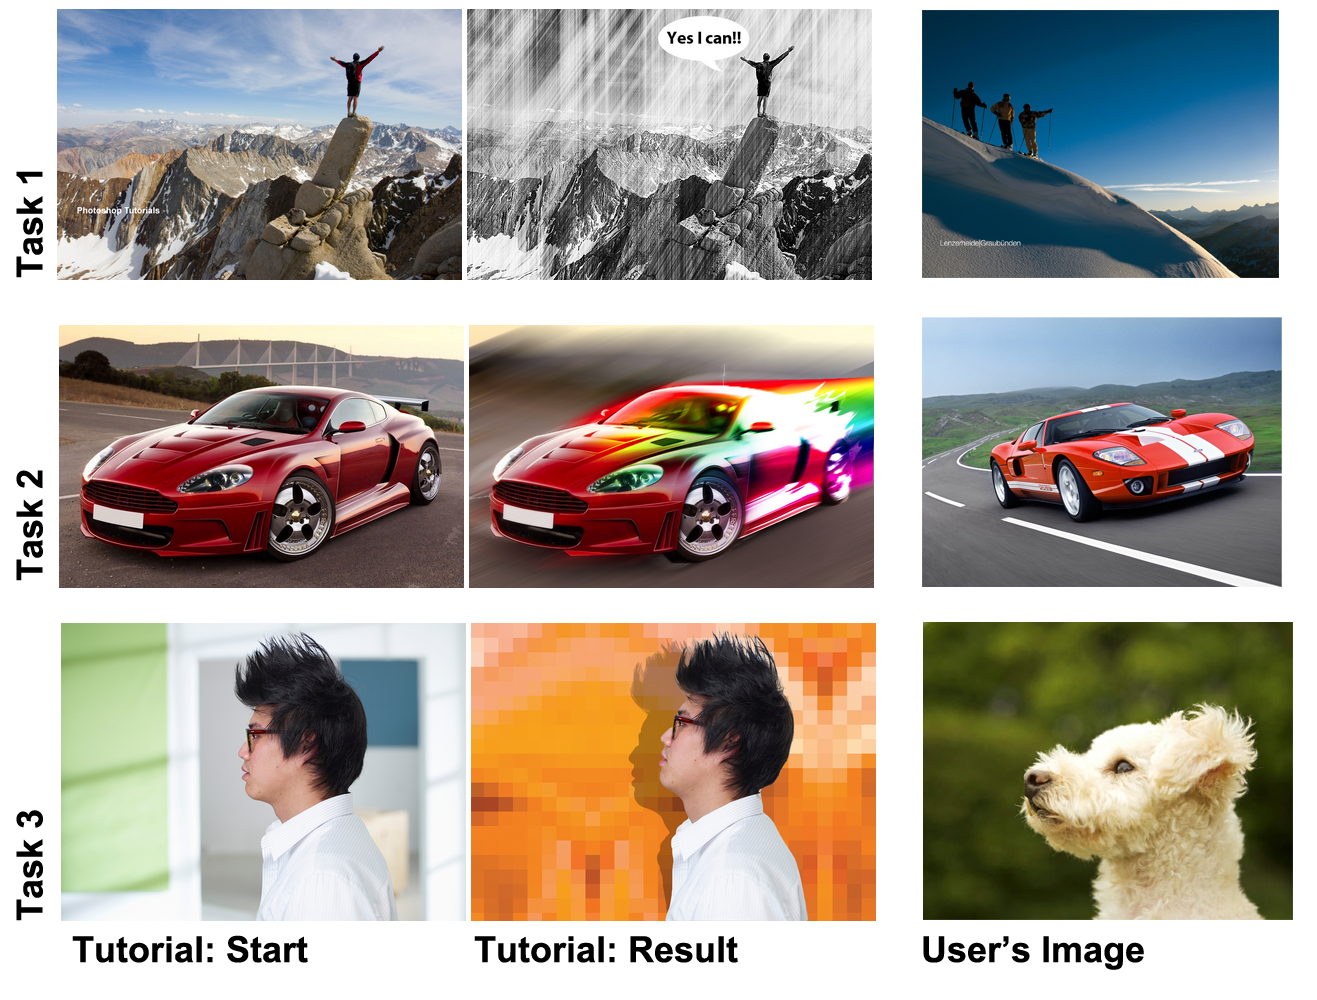
\includegraphics[width=\textwidth]{\mixt/fig/formative_study/study-images}
  \caption{In our formative study, participants completed three tutorials with images similar but not identical to the originals.}
  \label{fig:formative_tasks}
\end{figure*}

\begin{figure*}[t]
  \centering
  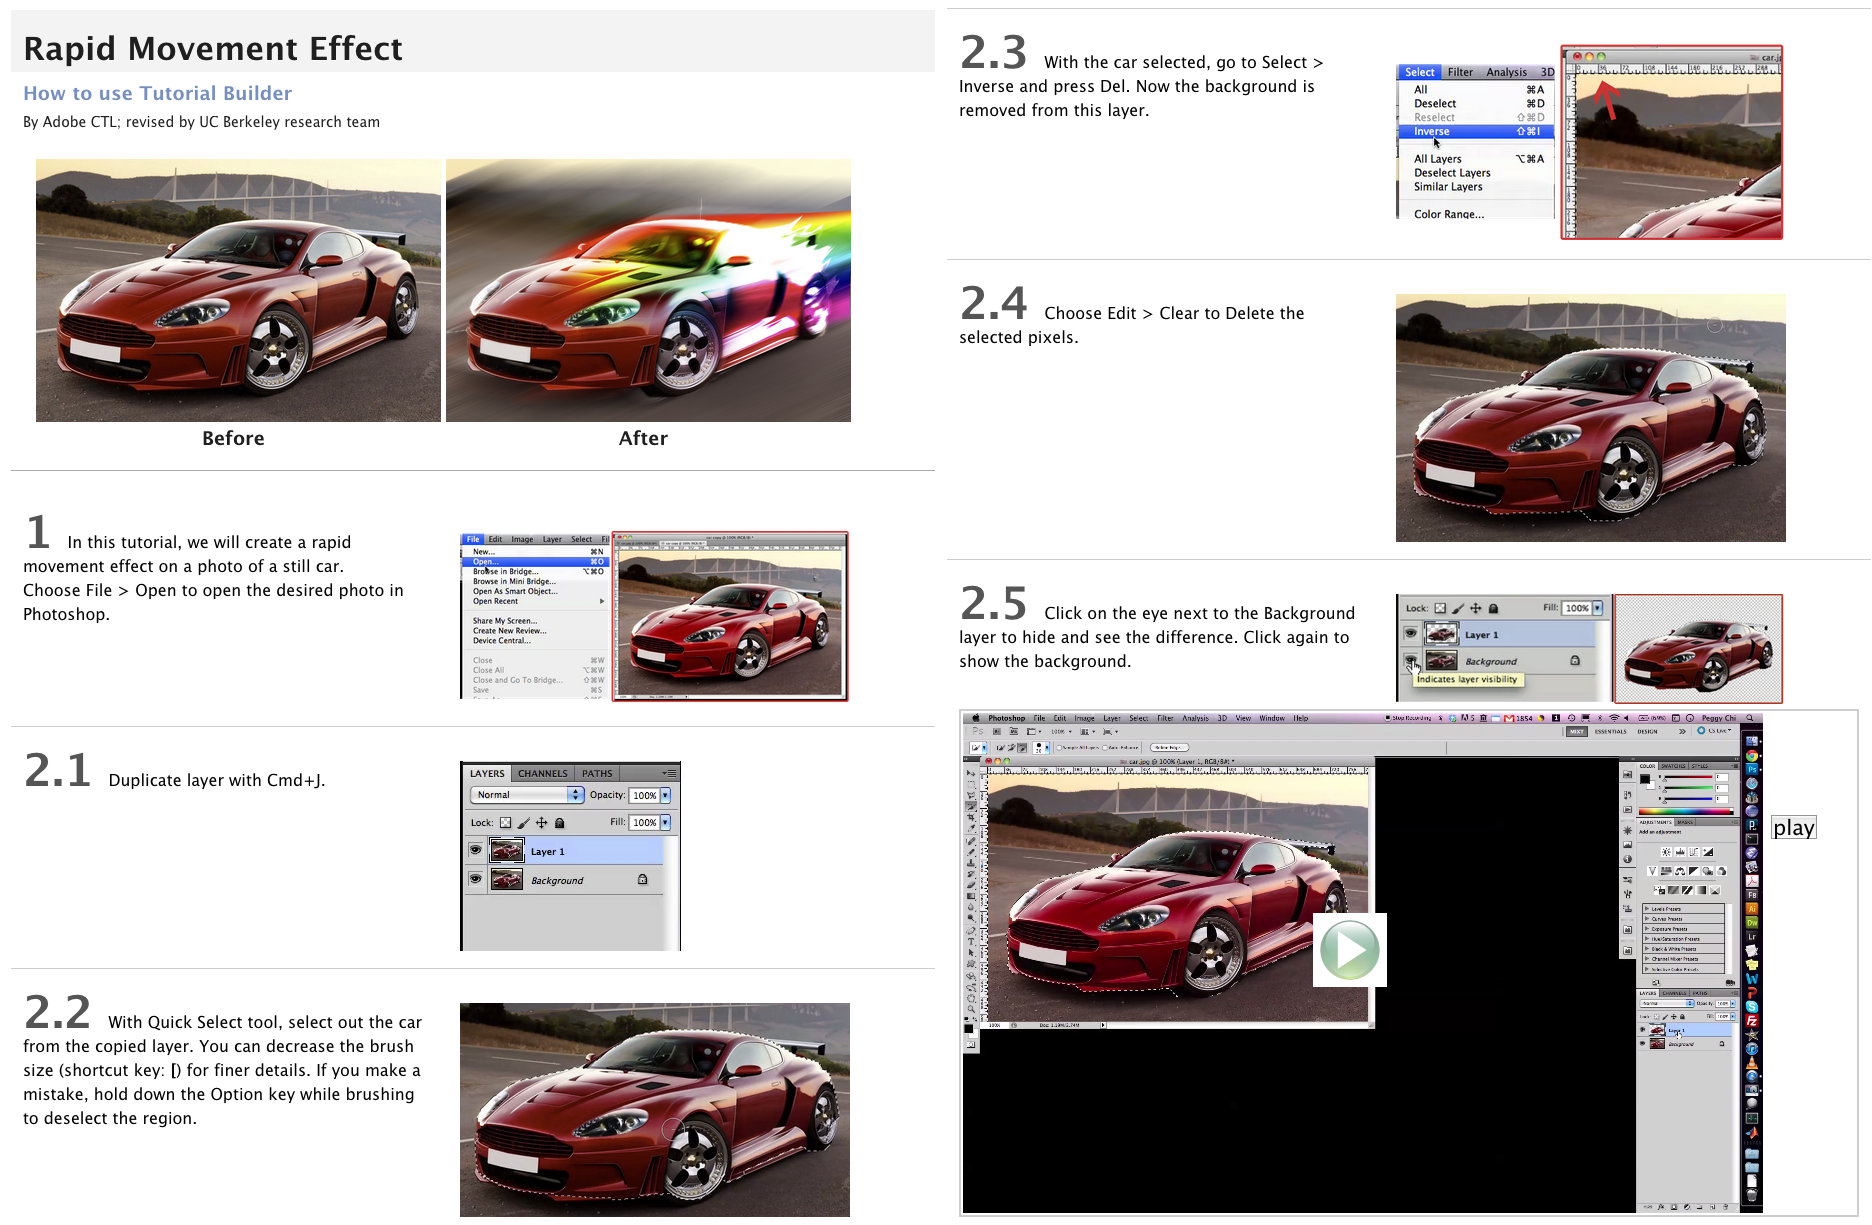
\includegraphics[width=\textwidth]{\mixt/fig/formative_study/study-mixed-example}
  \caption{In the mixed condition, participants saw an HTML page with static images and text; they could expand each step to view a video of that step (here: step 2.5).}
  \label{fig:formative_mixt}
\end{figure*}

% \subsubsection{Study Design}
\subsubsection{Hypothesis}
Our formative study aims to test the following two hypotheses:

H1: Image manipulation tutorials that mix static images and video clips are more effective than all-static or all-video tutorials.

H2: Users benefit more from seeing video clips instead of static text and images for certain types of commands.

\subsubsection{Participants}
We recruited 12 participants (5 males and 7 females, aged 20-52), 4 from a campus student design group and 8 from a computer software company, and compensated each with a \$15 gift card for participating. Our tutorials focused on achieving specific tasks in Adobe Photoshop. We recruited participants who had prior expertise with Adobe Photoshop, but who were not expert users. To demonstrate expertise, potential participants first completed an online screening test that asked them to follow a short image manipulation tutorial and submit the resulting file. The selected participants had between 1 and 20 years of experience using Photoshop.

\subsubsection{Tasks and Material}
The study was based on a within-subject design. We looked through Photoshop books and selected 3 different image manipulation tasks with similar levels of difficulty and complexity (see Figure~\ref{fig:formative_tasks}). Each tutorial comprised 15-20 steps. We focused on tutorials that included new, less common features such as the liquify tool, gradient warp tool, and puppet warp tool to increase the chance that participants would encounter unfamiliar tools. For each tutorial, we created three types of presentations: 1) static (in HTML format displayed on the screen), 2) video (on YouTube with audio narration), and 3) mixed (web interface shown in Figure~\ref{fig:formative_mixt} without audio). To ensure that different formats presented equivalent information where possible, we first recorded and narrated our video tutorials, then manually generated the static version by writing text instructions based on the narration and annotating and cropping frames of the video. To create mixed tutorials we started with the static tutorials and added the corresponding screencapture video segment for each step. To view the video segment for a step in the mixed tutorial, the user had to click on the image for that step. We scaled these videos to a fixed resolution of 800x500 pixels so that at least 2-3 steps would fit on screen when the videos were expanded. Many online tutorials do not offer full-screen resolution videos; even when high-resolution videos are available, they are hard to use as they force users to continually switch between the video and application windows. We disabled the soundtrack in the mixed tutorial to avoid situations when users only relied on auditory instructions instead of learning from static or video formats.

For each task, participants were given a source image that was distinct, but thematically similar to the image manipulated in the tutorial itself. This study design choice was motivated by the fact that users typically want to transfer the techniques found in tutorials to their own images.

\subsubsection{Procedure and Environment}
Each session consisted of 1 warm-up task and 3 experimental tasks. The warm-up task was a short 5-step static tutorial. In the 3 experimental tasks the format and task order were randomized. Each 60-minute session was conducted in a lab environment, using computers running Mac OS X, Adobe Photoshop CS5.1 and a web browser (Google Chrome) for viewing tutorials. Each participant was provided with a keyboard and a mouse and was allowed to adjust the equipment setting such as the monitor position and mouse tracking speed during the warm-up task. Photoshop and the web browser were arranged side-by-side on a 30-inch monitor with a resolution of 2048x1280 pixels. During the study, we used screen capture software to record user performance.

\subsubsection{Measurement}
To evaluate H1, we report the number of errors and repeated attempts that the participants made for each task. While our ultimate goal is skill acquisition and retention, we focus on the pragmatic goal of improving users' success in following tutorials and performing the instructions. We record an error if the participant performed a command incorrectly or skipped a step in the tutorial. While errors give a sense for the effectiveness of the tutorials, they do not measure the extraneous work users might have to perform when they have trouble understanding the correct outcome of a step. For example, if a user makes an error and then correctly executes several steps before recognizing the problem, we count this as a single error, even though the user must go back to fix the problem and then redo the subsequent steps. In addition, users may select the right command, but be dissatisfied with the result of their image and try again (e.g., redrawing a gradient). In such cases, we record all executions of the same step following the first attempt as a repeated attempt. Note that we do not count adjustments of continuous parameters or refinements of selection regions as repeated attempts because in these cases, the user is focusing on a single action rather than repeating a previously executed step. We do count a repeated attempt if the user entirely undoes a step to then retry it.

To evaluate H2, we count the number of different users who click on the video for each step in the mixed tutorials. To determine whether some types of commands benefit from videos more than others, we bin each step into one of the following five command categories based on the types of user interaction and UI elements it involves: brushing/drawing, manipulating control points (e.g., mesh-based warping, spline editing), parameter adjustment (e.g. using a slider to change opacity), UI navigation (e.g., switching tools, finding menu items), and layer operations.

We also collect qualitative data by observing how users follow the presented information and obtain additional feedback via 5-point Likert-scale questions (e.g., “The {\textless}condition{\textgreater} tutorial was easy to follow.”) and open-ended questions (e.g., “Compared with static tutorials, what were the pros and cons of the mixed media tutorial?”).

%!TEX root = ../thesis.tex
\subsection{Results of Formative Study}

\begin{figure*}[t]
  \centering
  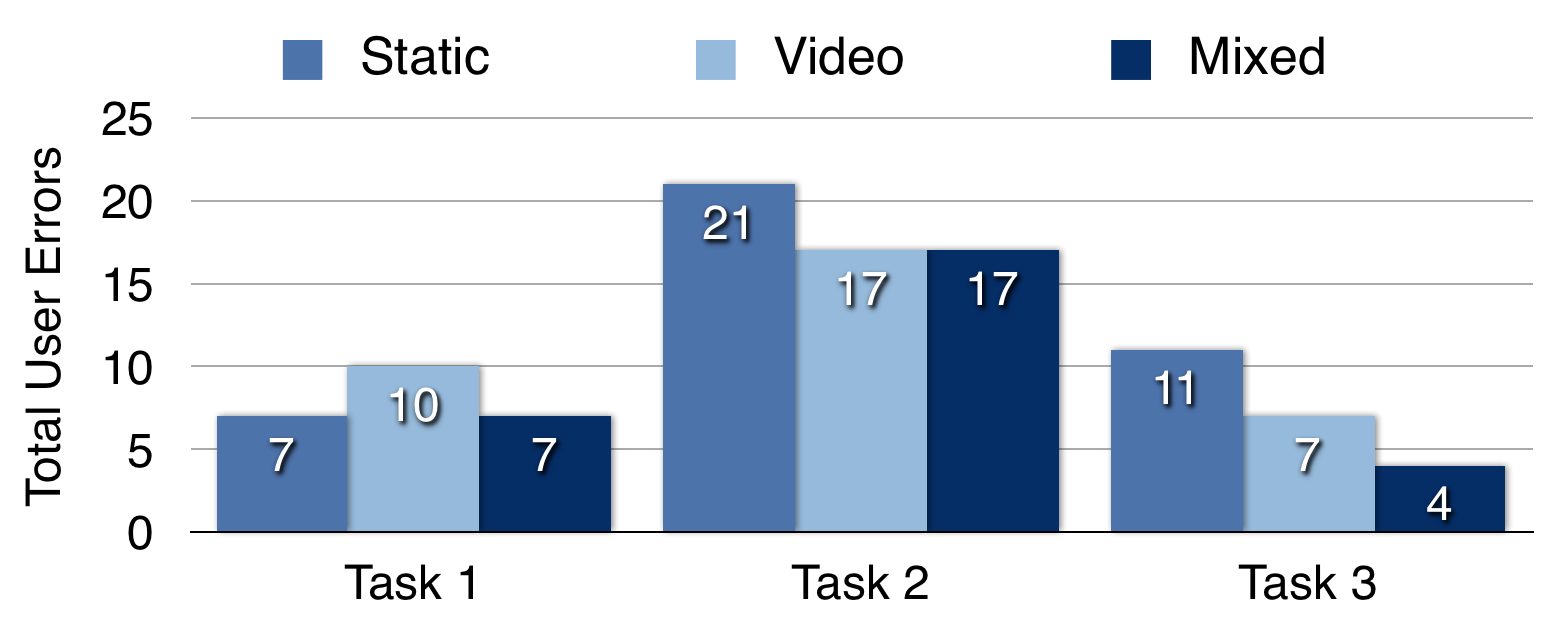
\includegraphics[width=0.5\textwidth]{\mixt/fig/formative_study/study-errors3}
  \caption{Users tied for fewer errors with mixed tutorials.}
  \label{fig:formative_errors}
\end{figure*}

\begin{figure*}[t]
  \centering
  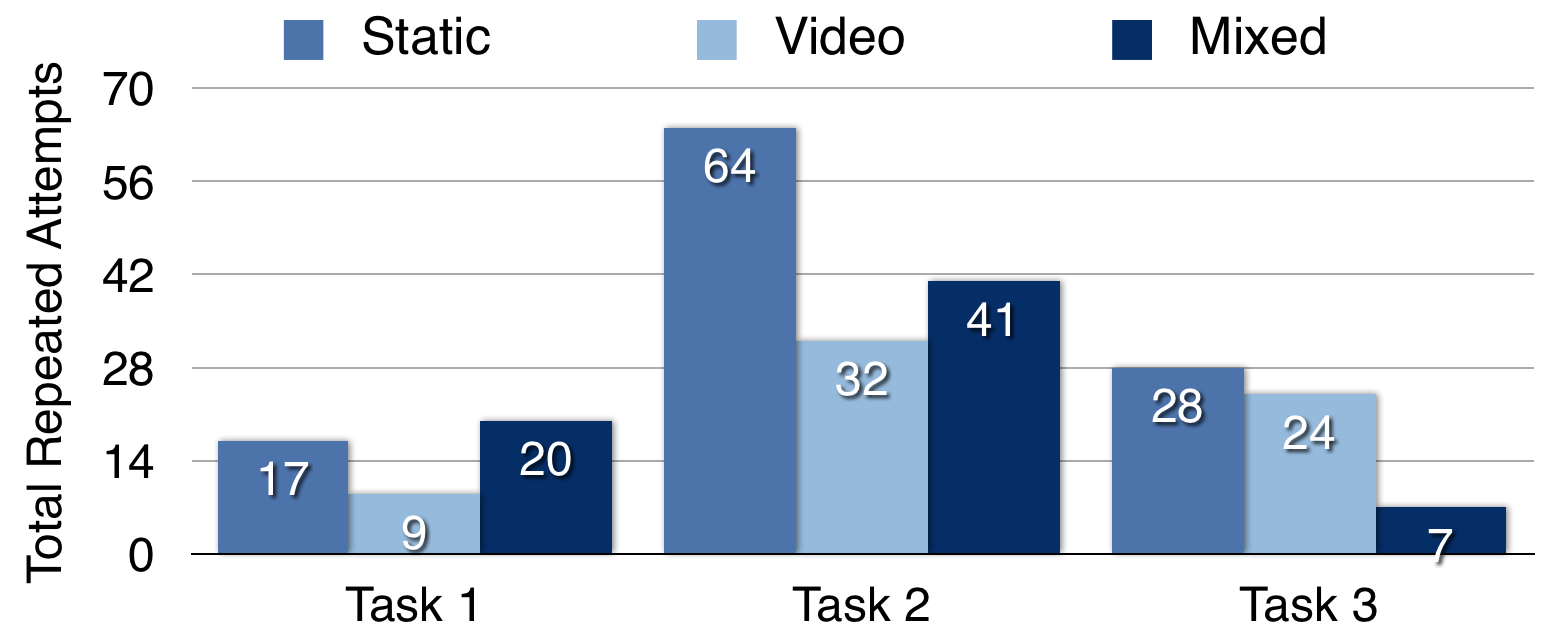
\includegraphics[width=0.5\textwidth]{\mixt/fig/formative_study/study-repeats3}
  \caption{In two of three tasks, participants made more repeated attempts at executing steps with static tutorials than with mixed tutorials. Video tutorials had the fewest attempts.}
  \label{fig:formative_attempts}
\end{figure*}

Based on the quantitative data and observations from our study, we gained several insights about how users interact with static and video content.

\subsubsection{User Performance on Image Editing Tasks}
Our analysis of user performance supports \textbf{H1}. As Figure~\ref{fig:formative_errors} shows, mixed tutorials resulted in the fewest total number of errors (28 for mixed, 34 for video, 39 for static) across all three tasks and produced an equivalent or fewer number of errors compared to static and video for any given task. In terms of extraneous work, the mixed condition resulted in many fewer repeated attempts than static tutorials and slightly more than video tutorials (65 for video, 68 for mixed, 109 for static, see Figure~\ref{fig:formative_attempts}). Although the differences in errors and repeated attempts are not statistically significant–-likely due to the small study size and differences between the tasks-–the overall trends suggest that mixed tutorials help users make fewer errors and do less extraneous work compared to static and video tutorials.

In addition to these quantitative results, we observed a few specific behaviors that had an impact on user performance:

The scannable nature of the static and mixed tutorial formats helped users follow along and avoid missing steps that might result in errors. In the video condition, users were more likely to accidentally skip steps because they were working at a different pace than the video. They also had trouble finding previous steps when trying to identify the source of an error.

In the static condition, users had trouble understanding how to perform steps that involve complex or unfamiliar UI elements and interactions. As we discuss in the following subsection, these were often the same steps where users decided to play the videos in the mixed condition. With only static text and images, users often made errors or had to repeat such steps multiple times.

Participants used the video clips in the mixed condition in a few different ways. Some users played the video \emph{before} attempting the step to familiarize themselves with the relevant UI elements and interactions. In some cases, users also played the video at the same time as they performed the action, which corresponds to what Palmiter and Elkerton described as ``mimicking actions'' \cite{Palmiter:1991:ADV:107792.107797}. We suspect both of these behaviors helped reduce errors, especially for complex or unfamiliar steps. In addition, several users also played the video \emph{after} completing a step, as a way to confirm that they had performed the step correctly and “debug” what went wrong if they made an error. This confirmation behavior helped reduce repeated attempts by making it easier to recognize and fix errors sooner.

In some cases, users had trouble seeing all of the relevant details in the mixed videos because the videos were scaled down to 800x500 pixels. For example, when using the \emph{puppet warp} tool, users missed that dragging in the vicinity of a control point (instead of on top of the control point) initiated a control wheel for a rotation rather than a translation maneuver. Although participants neither complained about not being able to resize the video in the MixT condition nor chose full-screen mode in the video condition, they explained that they would hope to clearly see the key part of the demonstration video.

\begin{table}[t]
  \centering
  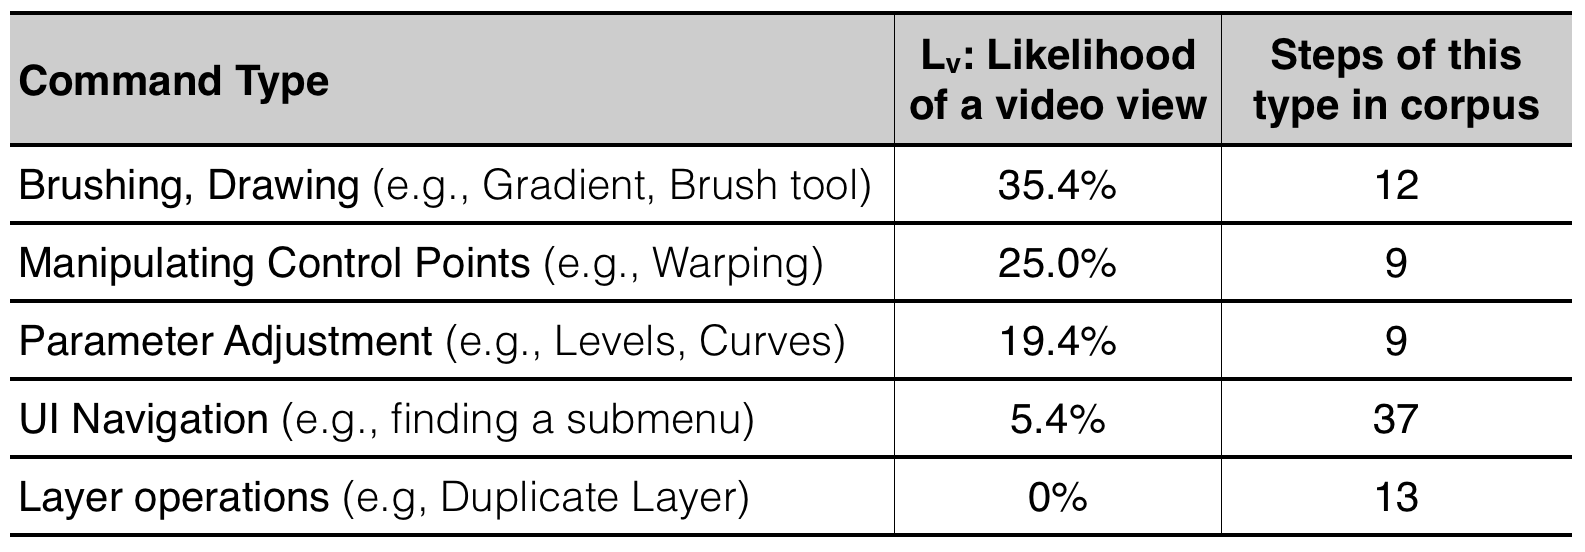
\includegraphics[width=0.8\columnwidth]{\mixt/fig/formative_study/command-table2}
  \caption{Participants watched videos most often for brushing, control point manipulation, and parameter adjustments.}
  \label{tab:formative_video_views}
\end{table}

\subsubsection{Which Commands Led to Video Views?}
Our analysis of which mixed steps prompted users to click on the corresponding videos suggests that users did indeed find the video clips more beneficial for some types of steps over others (\textbf{H2}). To compute the \emph{likelihood of a video view} ($L_V$) for the five command categories described earlier, we first determine $L_V$ for each individual step (across all three mixed tutorials) by computing the fraction of users who clicked to view the video for that step, and then we average likelihoods across all the steps in each command category.

As Table~\ref{tab:formative_video_views} shows, $L_V$ is highest for steps that involve brushing/drawing, manipulating control points and parameter adjustments. Based on our observations, videos help users perform the first two types of commands (brushing/drawing and manipulating control points) by explicitly demonstrating the necessary mouse movements rather than requiring the user to infer what to do from text and images alone. In addition, we noticed that some participants used the video clips to determine how precise they needed to be for certain brushing or selection tasks, which is hard to convey with a static representation. Text descriptions such as ``rough'' and ``detailed'' are relative and can be interpreted differently by individuals, but seeing how much time the demonstrator devotes to the task provides a much clearer estimate of the required precision for that task. As for parameter adjustments, users may be relying on the videos to provide some context about the range of visual effects the relevant parameters cover in order to determine what parameter values to use for their own image. Unlike static images, which only show the final parameter values and resulting effect, video demonstrations often show how the canvas changes as continuous parameters are updated (often via sliders), which may give users a better sense for the desired outcome of the step.

\subsubsection{User Preferences for Tutorial Types}
The results of our questionnaire show that while participants had varying opinions on the static and video tutorials, all users strongly agreed that the mixed tutorial was easy to follow. Participants had difficulty finding the tools that the static tutorials referenced and remarked that there were not enough visuals. For full-length videos, participants disliked having to pause the video to complete each step. For the mixed tutorial, half the participants found that video was the most useful among different media components for understanding a step instruction. One participant acknowledged that because the mixed tutorial allowed him to “break down the process into simple steps,” he was able to easily find the point where he had made a mistake. Another user explained that videos would be most helpful if the tasks were more advanced and in-depth. On the other hand, users had different preferences within a task. Expertise could be tool-specific: users might find static instructions sufficient for one set of operations (e.g., duplicating layers), and needed to watch videos for another set they were less familiar with (e.g., the \emph{puppet warp} tool). Overall, these responses suggest that users appreciated being able to choose from static and video features in mixed tutorials.



%!TEX root = ../thesis.tex
\subsection{Design Guidelines}

Based on the findings from our formative study, we propose four design guidelines for creating effective mixed media tutorials that combine text, images and videos.

\subsubTitleBold{Scannable steps} Scannable steps provide valuable context and facilitate navigation within tutorials. To leverage these benefits, videos in mixed tutorials should be presented in a format that supports scanning.

\subsubTitleBold{Small but legible videos} To make mixed media tutorials scannable and enable users to work with the tutorial and their application side-by-side, the videos for individual steps should use the minimum amount of screen real estate while still being legible. Ideally, videos should clearly depict the most important portions of the UI for each step (e.g., dialog boxes, panels, or canvas) while hiding or deemphasizing less relevant regions.

\subsubTitleBold{Visualize mouse movement} Our study indicates that videos are most useful for steps that involve brushing, drawing and manipulating control points, but even in videos, it can be difficult to see the exact motion or path of the mouse during such interactions. Visualizing mouse movement and events helps viewers understand the relevant spatio-temporal characteristics of the demonstration.

\subsubTitleBold{Give control to the user} Our observations of user behavior suggest that expertise and familiarity with the specific tools or interactions in a tutorial is likely to have an impact on which instructional format (static or video) is best for a given user. Videos help users understand, confirm and debug steps with unfamiliar tools, while static images and text are quicker and easier to skim. Thus, mixed tutorials should let users choose the most appropriate format at the granularity of individual steps.

%!TEX root = ../thesis.tex
\section{Computer-Generated Mixed Media Tutorials}

The benefits of mixed media tutorials are unlikely to be realized if creating such materials is too tedious, time-consuming, or if it requires more expertise than creating other tutorial formats. To lower the authoring barrier, we designed MixT, a system that automatically generates mixed media tutorials from user demonstrations. While the MixT architecture can apply to different media creation applications, our current implementation is specific to creating interactive tutorials for Adobe Photoshop.

\subsection{Overview}
\subsubsection{Tutorial Format}
MixT generates HTML tutorials with embedded videos that follow the design guidelines identified in our study. By default, our interface presents a textual description and screenshot for each step, just like a standard static tutorial (see Figure~\ref{fig:mixt_teaser}A). Clicking on the screenshot replaces the static image with a video player that plays the segment of the original demonstration that corresponds to the written step instructions. For example, a screenshot of a layer panel enhances the instruction ``\emph{Select Soft Light from the drop-down menu for Blend Mode},'' and the corresponding video clip shows continuous mouse action to the menu, expanding the drop-down menu, moving down to click on the feature, and shows the canvas change. By presenting steps as text and images with video clips that are accessible on demand, MixT tutorials retain the scannability of static tutorials while giving users the option of static- or video-based instruction at each step. To ensure that steps remain scannable and that the tutorial can still be viewed alongside the image editing application (without window switching), we scale each in-place video to at most 700 pixels wide and display text instructions on the left.

\subsubsection{Video Playback Options }
\begin{figure*}[b!]
  \centering
  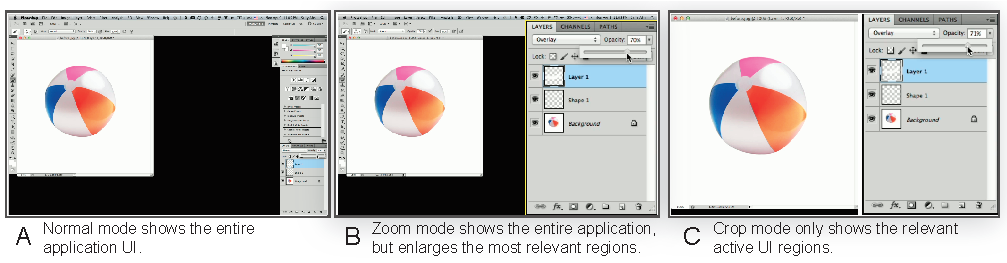
\includegraphics[width=\textwidth]{\mixt/fig/mixt_modes/Fig6}
  \caption{MixT offers three video playback options: Normal mode (A), zoom mode (B) and crop mode (C).}
  \label{fig:mixt_modes}
\end{figure*}

The MixT video player gives users additional control over the format of playback. Three different modes (normal, zoom, and crop) each emphasize different types of information (Figure~\ref{fig:mixt_modes}). In addition, users can display a pointer trace visualization to clarify the path of mouse interactions.

\emph{\textbf{Normal mode}} shows the entire application window (Figure~\ref{fig:mixt_modes}A). This mode preserves all context, but because MixT scales videos down to at most 700x440 pixels positioned next to the text instructions, it may be hard to see precise manipulation or small widgets or handles in the UI.

\emph{\textbf{Zoom mode}} also shows the entire application window, but performs a non-uniform enlargement of specific UI regions. In particular, the application area being manipulated (e.g., a menu, dialog, or the canvas) is enlarged to fill the full height of the frame and composited on top of the original video in another video layer (Figure~\ref{fig:mixt_modes}B). If a dialog also modifies pixels on the canvas, both areas are enlarged and positioned such that they do not overlap. This video composition effectively creates a focus-plus-context view that makes important regions easier to see at a given video resolution \cite{Furnas:1986:GFV:22627.22342}. Commercial screencasting software commonly includes a pan-and-zoom technique to make interactions legible in small videos. However, testing early prototypes of MixT suggested that such a technique is not appropriate for brief, single-step videos, as it is hard to establish application context in such short video segments.

\emph{\textbf{Crop mode}} does not show the entire application — it only shows the currently active area (a tool bar, dialog, main menu, or a panel) and the canvas if being changed (Figure~\ref{fig:mixt_modes}C). This offers the unique benefit of showing both a user interface manipulation (e.g., moving a layer opacity slider), and the effect on the image (e.g., parts of the image becoming transparent), while minimizing all other visual distractions. Like the zoom mode, cropped videos are very compact since only the relevant portions of the UI are shown.

\emph{\textbf{Mouse visualization}}: To help video viewers understand interactions with the canvas, MixT can render a trace visualization of the mouse (Figure~\ref{fig:mixt_mouse}). These traces show a fading path of the most recent positions of the cursor and encode mouse state using color: click events are shown in green (mouse down) and red (mouse up), while mouse \emph{movement} events are shown in purple, and mouse \emph{dragging} events are shown in yellow. Commercial screencasting software also includes mouse visualization techniques. However, they are usually limited to clicking, and the visualizations are typically rendered into the final video. In contrast, MixT emphasizes dragging because such interactions are especially relevant for image manipulation. Furthermore, our trace visualizations can be toggled on and off interactively in real-time. By default, the visualizations are enabled for all steps. However, users can change this behavior through an option in the video player.

\begin{figure*}[t!]
  \centering
  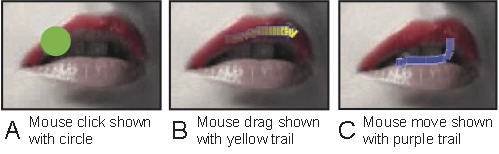
\includegraphics[width=0.7\textwidth]{\mixt/fig/mixt_mouse/mouse_visualizations}
  \caption{Mouse visualization distinguishes moving and dragging.}
  \label{fig:mixt_mouse}
\end{figure*}

%!TEX root = thesis.tex
% Pipeline of the DemoDraw system: technical details

\begin{figure}[t]
  \centering
  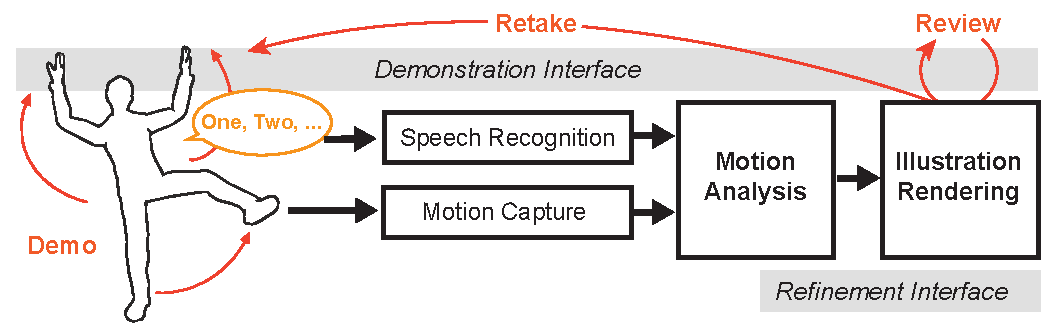
\includegraphics[width=0.8\columnwidth]{\demodraw/fig/pipeline/pipeline}
  \caption{\systemname{} System Components and Pipeline}
  % \dan{now that I understand the components better, we should emphasize motion capture component less since didn't make much contribution there.  I tweaked the figure to do this, and also highlighted the ``interaction pipeline'' (demo, review, retake) a bit better too.   }
  \label{fig:pipeline}
\end{figure}

\section{Generation Pipeline}

% \dan{I think we should downplay ``pipeline'' and emphasize ``system components'' ... pipeline sound very linear and non-iterative.}

%To support the described user scenario, we introduce our pipeline and system components shown in .
\systemname{} has four main components (Figure~\ref{fig:pipeline}):
%
a \emph{motion capture} engine to record joint data from the author's demonstration and apply it to a 3D avatar;
%
a \emph{speech recognition} engine to process speech input for commands and motion labels;
%
a \emph{motion analysis} algorithm to partition recorded motion and identify salient joint movements for each illustration segment;
%
and an \emph{illustration rendering} engine to visualize the avatar and motion segments with different effects.
% , and a module to handle user interaction.
%
% Our novel techniques enables motion segmentation by combining speech and motion inputs. Our interaction model allows users to modify the rendered illustrations interactively by demonstrations.
These components combine into an interactive and iterative system pipeline to translate demonstrations into motion diagrams.
A notable technical contribution is our motion segmentation algorithm combining speech labels and joint motion streams.
% \dan{I tweaked the two points above, old text is commented out in the tex}

% \dan{say something like our technical contribution is in motion segmentation (and maybe illustration rendering) }
%
\systemname{} is implemented using C\# in Unity 5. %\footnote{\url{https://unity3d.com}}.
It runs interactively on a Macbook Pro with Windows Bootcamp (2.5 GHz Intel Core i7 processor and 16 GB memory).
%
Below we describe the design and implementation of each component.

% ---------------------------------------------------------------

\subsection{Motion Capture}
% \dan{Call it ``Motion Capture'' component, with three sub components: Kinect, Avateering, and NPR}
% \bjoern{I moved NPR from capture to illustration rendering since it's a rendering technique.}
% \dan{good idea}

In support of our design goal to enable low-effort iteration within tasks, the motion capture component provides real-time feedback during demonstrations so authors can monitor their performance accordingly.
%\fixme{The raw joint data and RGB video stream are saved as csv and mp4 files for retrieval.}
%\dan{I put this here, but not sure we really need to state it at all. We don't really use the RBD video for anything either.}
% A central goal of our system is to enable average users to create illustration by physical demonstrations. As users might not necessarily have expertise to design illustration outcomes prior to a performance, it is important to provide real-time feedback for authors to observe the continuous motion captured effect and perform accordingly.
%
%\subsubTitleBold{Real-time Joint Data}
We capture position and joint angles of a simplified 25-joint skeleton using a Kinect2 sensor and the Kinect SDK 2.0. %\footnote{\url{https://dev.windows.com/en-us/kinect}}.
%Skeletal data of human body's 25 joints is captured in 3D, including head, shoulders, hands, and foot.
% At any given frame of motion capturing, our system gathers information about position, depth, and orientation values in meters for each of the 25 joints.
%Therefore, \systemname{} presents a 3D human model mirroring an author's movements in real-time while she stands in front of a Kinect sensor in a static, indoor scene (Figure~\ref{fig:pipeline}a).
%\dan{I commented a lot out here it didn't seem to add much beyond ``we capture using a Kinect'' (and just saying something like that is ok). }
%
%\subsubTitleBold{Motion Re-targeting}
The real-time joint data is applied to a generic 3D human model (an ``avatar'') using forward kinematics enabled by a modified Unity asset\footnote{\url{https://www.assetstore.unity3d.com/en/\#!/content/18708}}.
% \dan{I commented out a vague description of forward kinematics, I don't think we need it.}
% \bjoern{So the use of ``retargeting'' kinda raises a whole bunch of issues since motion retargeting is a big topic in animation. If bone lengths don't match between the actor's skeleton and the virtual model, contacts like clap or hand-on-head won't work. At a minimum state that we do not yet perform any smart retargeting to deal with changing segment lengths. I think the canonical reference is Gleicher~\cite{gleicher1998retargetting}.}
% \dan{yes, let's avoid saying ``retargeting''}

% When the motion data gets updated from the Kinect sensor, \systemname{} applies the joint information to a structured 3D human model (i.e., an ``avatar'') using forward kinematics in real-time. Given the human skeleton hierarchy from the body root (i.e., base spine) to the end of body parts (such as hand tips and feet), we compute the bone rotation angle to locate each joint to the target location in space. In this way, user can observe the avatar that follows her motion, which can also be viewed from any angle in a 3D space. This can be useful when user performs movements perpendicular to the Kinect camera \peggy{need a better way to frame this}.


% Based on our survey on existing practices of illustration design principles, it is important to make a character's appearance concise and clean. Often, outlining a human figure or showing in silhouette effectively preserves only essential information. Therefore, we apply Non-Photorealistic Rendering (NPR) techniques \cite{gooch1998non} to the 3D avatar in our engine that can be rendered and modified in real-time, including outline, silhouette, and flat-shaded colour (see Figure~\ref{fig:DemoDrawUI}-1d for examples).
% quaternion

% \subsubTitleBold{Implementation}
% This engine is implemented using Unity 5\footnote{\url{https://unity3d.com}} and the Kinect SDK 2.0 package\footnote{\url{https://dev.windows.com/en-us/kinect}} in C\#. Raw joint data and video stream from color frames are saved as csv and mp4 files for retrieval. Motion retargeting is achieved by a modification of a Unity asset\footnote{\url{https://www.assetstore.unity3d.com/en/\#!/content/18708}}. NPR shaders are applied to the 3D model for different rendering results.

% ---------------------------------------------------------------

\subsection{Speech Recognition}
Speech is used when recording a demonstration to label motions (e.g., ``one, two, ...'') and for recording and navigation commands (e.g. ``Start, Stop, Retake'' or ``Replay, Next, Play'') -- see Figure~\ref{fig:DemoDrawUI} for the speech commands that \systemname{} supports.
\dan{I made these consistent with new Figure 4}
%
We recognize both types of speech using the Microsoft speech recognition library\footnote{\url{https://msdn.microsoft.com/en-us/library/hh361572}} to process audio captured by the Kinect microphone array.
During recording, the start time, duration, and confidence of each motion label are logged for use in the motion analysis algorithm.
% https://msdn.microsoft.com/en-us/library/system.speech.recognition.recognizedaudio.starttime(v=vs.110).aspx
% \dan{how do you calculate delay? I thought this was a fixed constant determined by manual inspection.}
% \peggy{The api provides, but I didn't get to use it...}

%In addition, \fixme{a set of X voice commands} are recognized for non-sequential navigation .

%  addition to capturing and rendering user's continuous movements, \systemname{} considers instructor's existing practices of specifying motions using speech during a physical demonstration.
% By listening to the Kinect sensor's microphone array, \systemname{} integrates a speech recognition engine\footnote{\url{https://msdn.microsoft.com/en-us/library/hh361572}} to recognize user's speech input in real-time. Information of a detected spoken word, including the timestamp, delay, and confidence, is captured to be used for motion analysis and to support \systemname{}'s multi-modal interaction.
%
% Can implement: go more than one word and combine (e.g., turn to the right)

% ---------------------------------------------------------------

\begin{figure}[!t]
  \centering
  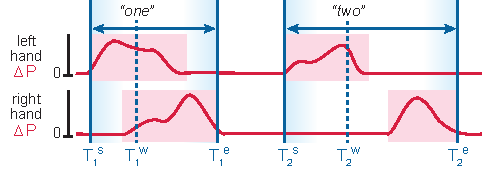
\includegraphics[width=0.8\columnwidth]{\demodraw/fig/motion_analysis/analysis2}
  \caption{Illustration of motion analysis algorithm (two joints shown due to space): significant moving periods of joint movements (pink) are mapped to speech labels to define motion segments (blue). Note the right hand period is mapped to \iquote{two} because it begins shortly after the left hand period.}
   \label{fig:segmentation}
\end{figure}

\subsection {Motion Analysis}
% \dan{Would be good to get a component name to include joint salience identification too.  ``Motion Segmentation and Joint Salience Identification'' component is too long, how about something more simple and general like ``Motion Analysis'' with subcomponents motion segmentation and joint salience.}

Our motion analysis algorithm translates a multi-part demonstration recording into a sequence of labeled time segments, each with one or more salient joint motions and a keyframe of joint positions for a representative body pose (see Figure~\ref{fig:segmentation} for an illustration of the approach).
Formally, given a set of $n$ speech labels $\{w_1, w_2, ..., w_n\}$ where each ends at latency-corrected time $\{T_1^w, T_2^w, ..., T_n^w\}$, our algorithm associates each speech label $w_i$ with a \emph{motion segment}, of which the start and end time are denoted as [$T_i^s$, $T_i^e$] where $T_i^s \leq T_i^w \leq T_i^e$. Each motion segment includes a set of $k$ salient joints $\{j_i^1, ..., j_i^k\}$ and keyframe time $T_i^{key}$ between [$T_i^s$, $T_i^e$].
It is then sent to the Illustration Rendering engine to create a motion illustration in a multi-part sequence.

Human motion segmentation and activity understanding has been well studied in computer vision and graphics \cite{Aggarwal:2011:HAA:1922649.1922653}. We adopted a spacetime approach to identify salient motion sequences in 3D space.
%
However, in our scenario such as dancing, movements may not necessarily encode a semantic meaning for automatic recognition, such as ``walking'' or ``throwing (a ball)'' in previous research. Therefore, our approach combines the user's speech labels, similar to a scene segmentation method used in DemoCut~\cite{Chi:2013:DGC:2501988.2502052}.
%
We make two assumptions about the synchronized data streams of speech labels and joint movements:
1) authors make short pauses between motions to be grouped, i.e., $T_i^e < T_{i+1}^s$, and
2) the speech label utterances overlap or closely occur with at least one joint motion;
% step-by-step movements are clearly segmented without an overlap.
%
These assumptions are practical since authors often pause for a moment to prepare for demonstrating the next movement in a step-by-step sequence.
% , or reposition their body without those movements being assigned to any label.

% where $T_s \leq T_w \leq T_e$,

% For a motion label detected by the speech recognition engine at time \(T_w\) (e.g., step ``One'' or a gesture ``Swipe''), \systemname{} automatically identifies an appropriate motion segment for visualization as follows: It analyzes the motion data in order to identify the start and end time of this segment [\(T_s\), \(T_e\)] where \(T_s \leq T_w \leq T_e\), a set of salient joints \({J_0, ..., J_n}\), and a representative pose at \(T_k\) associated with this speech label. Figure~\ref{fig:segmentation} shows one example of a right-hand movement segmented by the following approach: \bjoern{What instant in time does \(T_w\) represent? The beginning of a word? The end? Some time after the end of the word once recognition has completed? Seems fairly important - otherwise I have no idea if \(T_s \leq T_w \leq T_e\) is a reasonable assumption.}

% EUCLIDEAN DISTANCE
\subsubTitleBold{Motion Segmentation}
To determine a motion segment of [$T_i^s$, $T_i^e$] for each speech label $w_i$ that ends at $T_i^w$, we begin by identifying all \emph{moving periods} of significant joint movements (pink rectangles in Figure~\ref{fig:segmentation}) for 8 joints $J$: the 5 end-effectors (head, hands, feet), 2 knees, and the body root.
%
To filter jittery movements, joints are considered moving if smoothed inter-frame differences in absolute Euclidean distance are greater than a threshold.
%
Specifically, for each joint $j \in J$ of a frame $r$ at time $t$, the average difference in position between two adjacent frames $\Delta P = |P^r-P^{r-1}|$ is computed over the subsequent half second (15 frames).
%
If this moving average is greater than 0.05$m/s$, then joint $j$ of a frame is labeled as ``moving'', marked as $m_j^r$.
This is repeated on all frames and all joints.
Next, of the entire motion recording for joint $j$, we combine all the consecutive $m_j^r, m_j^{r+1}, ...$ into a joint moving period $M_j$.
% \dan{any extra hacks to join or filter out very small periods of movement like just a few frames? If so, explain here.}

Once a list of moving periods $\{M_j^1, M_j^2, ...\}$ for joint $j$ is determined, we begin labeling each $M_j^m$ at [$T_{m}^s$, $T_{m}^e$] to map to a speech label $w_i$ at time $T_i^w$ where $T_m^s \leq T_i^w \leq T_m^e$. In other words, the speech utterance occurs during or near to a joint movement (illustrated as dashed lines crossing pink rectangles in Figure~\ref{fig:segmentation}).
%
% Salient joint marking covered in the next paragraph ...
%Mark \(J_i\) as salient.
%
% If a movement overlaps with two labels (i.e., a continuous movement without a pause in between beyond our general assumption),
%
% \dan{do you have any rules to prevent a period of joint movement to be mapped to multiple speech labels?}
%
% Any unmapped periods ending less than $\epsilon$ before a motion label time, where $\epsilon = $ 1s defined earlier, or beginning less than $\epsilon$ after a motion label time, are also mapped to that label.
% \dan{See if what I wrote above makes sense, I was trying to interpret ``or 2) if an earlier segment that ends within a pause threshold is not mapped. A second pass of analysis after recording will examine if a segment shown after the label should be mapped to this label.'' }
%
% \fixme{After all the moving sequences of a joint is identified, \systemname{} concatenates these elements and finds the earliest frames at \(T_s\) and latest frame at \(T_e\) as the start and end times of this motion segment. Mark this as a salient joint \(J_i\).} \bjoern{revisit - i find this unclear, but I'm also tired.}\dan{I can't figure it out either, but I think it needs to be explained here}
%
After all moving periods are mapped to speech labels for all major joints, the start and end time [$T_i^s$, $T_i^e$] of the motion segment for label $w_i$ are set to the minimum start time and maximum end time across all mapped joint movement periods.
%as [$\min_{\forall j \in J} T_jm^s$, $\max_{\forall j \in J} T_jm^e$].
% \dan{the sentence above is my guess at what this means (same as what Bjoern guessed)
% ``Our algorithm repeats this segmentation for all the major joints. If there are multiple salient joints, combine and adjust [\(T'_s\), \(T'_e\)] for this motion segment.'' \bjoern{How do you do the adjustment? do different joints have individual start and end times, or do you take the min of all start times and the max of all end times?}}

\subsubTitleBold{Joint Salience Identification}
The salient joints $\{j_i^1, ..., j_i^k\}$ are defined by the set of all joints that were mapped based on significant moving periods.
% \dan{any other rules or hacks to do this?}

% \systemname{} analyzes a motion recording for significant motion changes using spatial thresholding of key joints. To concisely visualize body motion, we selected a subset from the 25 joints by their relative distance of a human body. For example, shoulder center can be represented by the head movement, and therefore trace only the latter joint. \bjoern{This is vague - which joints did you select? Why is this ``concise''? I don't understand the sentence about shoulders and heads at all. Maybe show a figure and highlight which joints you check.}
%
% For each joint, we calculate the Euclidean distance of joint locations in adjacent frames: $\Delta P = |P_t-P_{t-1}|$. If the average distance of a consecutive sequence within a moving window (set as 2 seconds) is over a difference threshold, it labels this as a moving joint sequence. \bjoern{what do you mean by average distance? do you just add up all frame differences for 2 seconds and divide by \# of frames? What is the difference threshold you empirically determined? What are the times $[T_{start},T_{end}]$ you find? }

% MATCH WITH SPEECH + FIND IN/OUT POINTS
% Next, our algorithm maps a moving joint sequence to this speech label if: 1) the sequence in time overlaps with the label's time \(T_w\), i.e., the movement is continuing, or 2) if an earlier segment that ends within a pause threshold is not mapped. A second pass of analysis after recording will examine if a segment shown after the label should be mapped to this label.
% %
% After it identifies all the moving sequences of a joint, \systemname{} concatenates these elements and finds the earliest frames at \(T_s\) and latest frame at \(T_e\) as the start and end times of this motion segment. Mark this as a salient joint \(J_i\). \bjoern{revisit - i find this unclear, but I'm also tired.}

% MULTIPLE JOINTS
% \subsubTitleBold{Joint Salience Identification}
% Our algorithm repeats this segmentation for all the major joints. If there are multiple salient joints, combine and adjust [\(T'_s\), \(T'_e\)] for this motion segment. \bjoern{How do you do the adjustment? do different joints have individual start and end times, or do you take the min of all start times and the max of all end times?}

% KEY FRAME
\subsubTitleBold{Key Pose Selection}
A key pose is used to represent a motion segment in an illustration. Based on our informal experiment, it is often the end state of movements as motion arrows are pointed toward this end goal (see the Figure~\ref{fig:pipeline} for example). Therefore, we set a key pose at a time near the end of a motion segment, specifically $T_i^{key} = T_i^e - 0.5$ second.
% \dan{should mention keyframe position in formative study section}
% \peggy{confirmed, and in figure 2}
% Therefore, we selects a frame \bjoern{x frames} from the out point \peggy{no intelligence here... how do we better describe?}.

\subsubTitleBold{Motion Retake}
When retaking a partial demonstration with one or more speech labels $\{w_i', w_{i+1}', ...\}$, the full motion analysis algorithm is run on the new recording. New motion segments then replace the original segments by mapping $w_i'$ with $w_i$.

% ---------------------------------------------------------------

\subsection{Illustration Rendering}

The Illustration Rendering engine generates a motion illustration for each motion segment of speech label $w_i$ (bounded by [$T_i^s$, $T_i^e$]). There are two related rendering tasks: the body pose and the motion depiction style.

\subsubTitleBold{Body Pose}
The body pose is determined by all joint positions at keyframe time $T_i^{key}$.
We use standard Non-Photorealistic Rendering (NPR)~\cite{gooch1998non} techniques to render the 3D human model in a stylized manner that abstracts away distracting details. Specifically, we support contour-only, filled silhouette, and flat-shaded rendering styles
% Following the principle of clarity through simplicity, Non-Photorealistic Rendering  \cite{gooch1998non} algorithms are used to render the 3D human model as a contour, silhouette, or flat-shaded colour
(see Figure~\ref{fig:DemoDrawRefinementUI}a left for examples).
% \dan{any more details? Unity asset used? tuning parameters? Is it fast?}

\subsubTitleBold{Line and Arrow Depiction Style}
Based on Cutting's criteria~\cite{cutting_representing_2002} and our survey of motion illustrations, we use lines with arrowheads as the default depiction style for visualizing joint movements.
This style is rendered as follows:
%
For each salient joint of a motion segment, the absolute joint positions in world space over the period [$T_i^s$, $T_i^e$] are used to construct a 3D poly-line using Catmull-Rom interpolation.
% \dan{can smoothing still be turned off?}
% \peggy{current not}
Two 3D cones are positioned collinear with the last two polyline positions to form arrowheads for both the beginning and the end of a line.
%
Although the poly-line is 3D, it is shaded to appear 2D.
%
All arrows are colored red by default to contrast with the avatar, a common technique for layering information~\cite{tufte1990envisioning}.
% \dan{and rendered to be always ``in front'' of the body.}
% \peggy{currently does not consider camera viewpoint, so no}

For some motions, visualizing absolute joint positions might not be suitable.
For example, for a two-foot jump with a two-hand waving motion (see Figure~\ref{fig:DemoDrawRefinementUI}c), our algorithm will mark all major joints as salient and generate multiple arrows showing the jump movement, but fail to convey the hand waving.
%
Authors can choose to visualize joint motions \textit{relative} to the spine instead,
triggering the same motion analysis algorithm described above to be re-run using relative motion.
In this way, the same movements would be shown more concisely with a single up arrow (for the overall jump direction) and two curve arrows (for the hand movements).
%The joint data will be re-computed based on the offset distance to the spine position. The result illustration, in this case, can be more concise by showing only the spine motion.

\subsubTitleBold{Other Adjustments}
Authors can review the results using the \phaseI{} or \phaseII{}. With the latter, line weight, arrowhead sizes, and color can be adjusted and re-rendered in real-time using graphical widgets (see Figure~\ref{fig:DemoDrawRefinementUI}a). Arrows can also be re-positioned to increase the offset ($\delta$) by direct manipulation dragging.
%
Considering some movements cannot be easily seen from the default front camera viewpoint (such as those parallel to the XZ plane, see Figure~\ref{fig:teaser}c top-right), our UI enables the selection of four other camera angles ($\theta$), including three-quarter front views (45$^{\circ}$ and -45$^{\circ}$) and profile views (90$^{\circ}$ and -90$^{\circ}$), all at the eye level. These discrete choices simplify control, but of course it would be possible to select any viewing angle given the 3D avatar and joint information. By default, 8 main joints are analyzed and illustrated, but any of the 25 body joints can be explicitly selected for illustration using the interface.

\subsubTitleBold{Stroboscopic Depiction Style}
Cutting~\cite{cutting_representing_2002} noted stroboscopic effects are also effective, and we found examples of illustrations with a sequence of overlaid semi-transparent body poses in our survey.
%
Therefore, authors can select a stroboscopic depiction style in the \phaseII{} (see Figure~\ref{fig:DemoDrawRefinementUI}b).
The style is rendered by compositing multiple semi-transparent renderings of intermediate body poses between $T_i^s$ to $T_i^e$ behind a rendering of the representative pose at keyframe time $T_i^{key}$.
Authors can adjust the number of intermediate poses $n$ (the default is 3 poses) and the horizontal overlap ratio $\rho$ between intermediate pose renderings can be adjusted to stack them up ($\rho=100\%$) or spread them out ($\rho=0$ is the default).

% Authors can then selectively combine these frames by specifying visual parameters, including numbers of frames to show, distance between frames, and whether to apply motion arrows. Our system will automatically adjust the distance and transparency values of selected frames and compose into a diagram.

\subsection{Results}
The \systemname{} pipeline is capable of generating expressive and clear motion illustrations. In Figure~\ref{fig:teaser}c, motion arrows show the upper body motion (top left), hand waving back and forth (top middle), and hand circular motion (bottom right). Whole body motions can also be visualized (bottom left), and can be especially helpful when motions are best viewed from a different angle, such as the side view (top right).
%
In Figure~\ref{fig:teaser}d, stroboscopic effect depicts the transition from the start pose to the end pose, which can be rendered as a sequence (top left) or in one combined pose (bottom left). A combination of this effect with motion arrows creates a compact, integrated illustration (top and bottom right).

% \dan{Talk about how expressive this pipeline is referring to diagrams shown in figure 1, the appendix, etc.}

\dan{Disclose what happens if assumptions don't hold or other problems with the pipeline. (this paragraph may migrate elsewhere).}

% ---------------------------------------------------------------

% -- Rebuttal --
% * Camera positions can present motion parallel to the XZ plane (R1), see Fig 1c top-right.
% * We do not embed color coding (R1,R2); we integrate "CMC l:c color differencing" to automatically avoid arrow colors visually similar to avatar colors.
% * 8 major joints are selected to give users higher-level control, but the system tracks all 25 detailed joints that can be revealed via the Refinement UI (R2).
% * Arrow path points are not sampled before Catmull–Rom interpolation (R1). It's simple, but it works because motions are often taken in 0.5s to 1s. We agree that sharp direction changes could be smoothed over: we can discuss alternate sampling methods like finding points with local min/max derivatives.

%!TEX root = ../thesis.tex
\subsection{Results}

\begin{figure*}[!t]
  \centering
  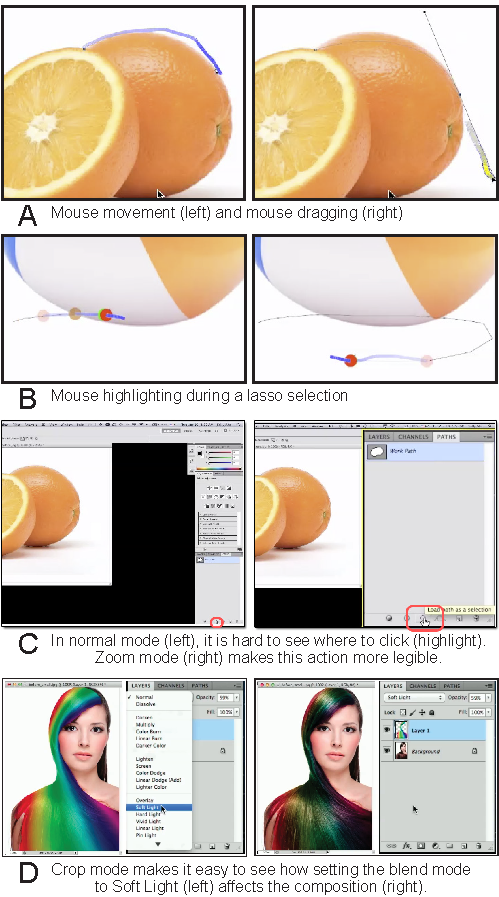
\includegraphics[width=0.95\textwidth]{\mixt/fig/mixt_results/mixt_results}
  \caption{Automatically-generated MixT results.}
  \label{fig:mixt_results}
\end{figure*}

We gathered nine different tutorials and recorded working through each tutorial in Photoshop. We then used MixT to automatically generate mixed media tutorials from these demonstrations. This section describes this corpus. The following section then evaluates the generated tutorials quantitatively and qualitatively.

Our tutorials came from both online and book sources: two from ``Adobe Photoshop CS5 Classroom in a Book,'' five from photoshopstar.com, one from makeuseof.com, and one from icanbecreative.com. All are popular resources for Photoshop learners. Two of the tutorials were also used in the formative user study. The selected tutorials had a total of 165 steps and covered all five command types: they contained 15 brushing/drawing operations, 14 control point manipulations, 30 parameter adjustments, 67 UI navigations, and 39 layer operations. The demonstrations were recorded on three different laptops running Photoshop in full screen with native resolutions of 1680x1050, 1440x900, and 1280x800 pixels.

Overall, the MixT tutorials that we generated exhibit the desired characteristics that we identified in our formative study: scannable steps, small but legible videos, visualized mouse operations, and user control over presentation format. We highlight some interesting results generated by MixT and also refer readers to the provided video figure, which has additional examples.

\subsubTitleBold{Scannability} The step-by-step layout of our tutorials makes them easy to scan. For example, at a glance, we see that the tutorial ``Turning an Image into an Old Photo'' involves several adjustment layer operations, while the tutorial ``Creating Artistic Effects'' involves more parameter adjustments and brushing commands.

\subsubTitleBold{Mouse visualization} Our mouse visualizations help clarify several interactions. They clearly communicate the difference between clicking and dragging, a distinction that is fundamental to operations such as path manipulation but hard to glean from screen capture video. For example, Figure~\ref{fig:mixt_results}A shows the difference between moving around the contour of an object without drawing a path (left), and dragging a Bézier handle to adjust a path segment (right). Mouse trails and click markers were also useful for showing the trajectory of lasso selections (Figure~\ref{fig:mixt_results}B).

\subsubTitleBold{Zoom and crop modes} For many steps, the zoom and crop videos offer clear legibility benefits over the normal video mode. In our corpus, zoom mode was especially valuable for highlighting actions on small buttons that occurred near the frame boundaries, e.g., in the layers palette (Figure~\ref{fig:mixt_results}C right). Such operations are easy to miss in a normal, scaled video (Figure~\ref{fig:mixt_results}C left). Crop mode was useful in showing the effect that parameter selection has on the canvas. Figure~\ref{fig:mixt_results}D shows two successive frames that illustrate how changing a layer's blending mode affects the image. Enlarging the canvas in these modes also helps users see the details of effects, such as applying the eraser tool on the canvas to enhance the underlying layer (Figure~\ref{fig:mixt_mouse}).



%!TEX root = ../thesis.tex
\section{Evaluation}
To evaluate the DemoWiz design, we conducted a controlled experiment in which participants recorded and edited a demo video, and gave a presentation with the edited video. Specifically, we wanted to see if presenters would evaluate their own performances higher with the support of our augmented visualizations and control of timing.

\subsection{User Study}

\subsubsection{Baseline Condition: DemoWiz without Visualization}
Since DemoWiz allows for rapid editing of the video, it would have been unfair to compare it with a conventional video player without supporting any editing during the rehearsal phase. We therefore modified our system to serve as the baseline condition, providing participants with the same lightweight editing of the video in each condition. However, during presentation, the baseline condition was similar to a conventional video player that shows only the video without event timeline and augmented visualizations. It also did not support the \textit{stop} markers and \textit{text notes}, i.e., participants could only adjust playback speed of each segment and add variable length \textit{pauses}. During presentation, participants only saw the video with a traditional timeline. They could, however, pause (or stop) and resume the video manually at any time during playback.

\subsubsection{Study Design}
We conducted the study as a within-subjects design in a usability room. After recording and editing a video using the same system, each presenter gave a presentation with both systems to an experimenter. To control the effect of order and learning, we prepared two tasks that included similar interaction flows and counterbalanced the order of the two systems—DemoWiz and Baseline—-but we fixed the order of tasks. Even though presenting to a single audience member in a usability room is not the same as using the system with a large conference audience, it is important to control the tasks and presentation as closely as possible to understand the relative benefits of the system in comparison with a baseline condition.

For each condition, we observed and coded the \textit{timing} of narration that matched the video content and noted the time in seconds when an event was described \textit{before}, \textit{at}, or \textit{after} the action happened in the demo video. We also marked obvious \textit{breaks} between narrations, \textit{errors} when the narration was not about the current or following events (e.g., discussing actions in a different order than they actually occurred), and \textit{misses} when an important action was not mentioned. To avoid unconscious bias that might influence the coding of the videos, we neutrally named the recordings and coded them all in a batch. We focused on objective timing measurements as much as possible, measuring deviation from specific video events and their corresponding narrations down to a second. Finally, we gathered qualitative feedback through satisfaction and preference questionnaires.

\subsubsection{Participants}
We recruited 12 participants (10 males and 2 females) from a software company. However, we excluded the data from two participants (1 male and 1 female); one was due to a software bug during one condition and another was because the participant requested to restart a presentation in one condition. The average age of the effective 10 participants was 37.3 ranging from 24 to 64 years of age. We recruited participants who had experience at showing a software demonstration to an audience such as giving a presentation at a conference. Four participants were native English speakers and the rest were fluent in English. The expertise of participants included audio processing, computer graphics, human-computer interactions, machine learning, networking, and software engineering. Each participant was compensated with lunch coupons worth \$20.

\subsubsection{Procedure and Tasks} Each session consisted of one training task and two experimental tasks. For the training task, to introduce the common features for recording and editing the video, we designed a simple workflow of five steps to demonstrate editing of a slide using PowerPoint. The experimenter briefly demonstrated an example and then introduced the recording program that captured the screen. Participants were then asked to practice and record using the recording program.

The two tasks consisted of a similar sequence and interactions: 1) searching with Bing Maps to show the 2D map view and the Bird's Eye view, looking for a restaurant, and navigating to the interior view of a specific restaurant; and 2) searching with Google Shopping to show the search results with the Grid view, filtering and voting for reviews, and navigating the 3D product view of an espresso machine. For each task, we provided a specific scenario along with a list of subtasks. The experimenter walked through this list with participants to ensure that they could easily find the features that needed to be demonstrated. Participants were then asked to practice (3-5 minutes), record (about 2 minutes), and rehearse and edit (5-10 minutes).

To help simulate a conference setting where participants would not be able to present immediately after having recorded a demonstration, we inserted an intentional 1-minute gap between rehearsal and presentation. During this gap before giving the presentation, we asked participants to watch a conference showcase video. Participants were then asked to stand up and gave a 2-3 minute presentation to the experimenter in a usability room.

After each task, participants filled out a questionnaire of 8-10 questions asking about their experience (8 for the Baseline condition, and 10 for the DemoWiz condition). At the end of the session, an online questionnaire was provided for them to present overall preferences and leave comments. Each session lasted about 1.5 hours.

\subsubsection{Experiment Setup}
Each participant used a desktop computer running Windows 7, Expression Encoder 4 for screen recording, and a web browser for the DemoWiz user interface. A regular mouse and keyboard were provided, along with two 27-inch displays, one for editing (during rehearsal) and showing the audience view (during presentation), and the other for the presenter view on a stand-up table. The resolution of both displays was 1920×1200 pixels. The average captured screen area was 1311×857 pixels. In the presenter view, the video resolution was within 1000×600 pixels; in the audience view, the screencast videos were resized to fill the entire display with at least 100-pixel wide border in black. During the study, the experimenter stayed in the room, providing instructions and sitting behind the participants during the recording and editing phases.

% ---------------------------------------------------------------

\subsection{Results}
Ten participants successfully recorded, rehearsed, and gave a demo with both systems.

\subsubsection{Subjective Preference}
Figure~\ref{fig:demowiz_likert} shows the average subject responses (on the 7-point Likert scale) from presenters for both systems. We analyzed these subjective responses using a Wilcoxon signed-rank test. We found significant differences in responses for ease of narration (DemoWiz µ = 6.2 over Baseline µ = 4.5, \textit{p} = .018) and ease of presentation (6.4 over 5.2, \textit{p} = .048). We also found marginally significant differences in participants' overall satisfaction with their presentations (5.5 over 4.7, \textit{p} = .062). Participants also tend to agree that DemoWiz helped them interpret timing (6.1 over 4.4, \textit{p} = .067).

In addition, 9 out of the 10 participants preferred DemoWiz to the system without visualization and would choose to present with DemoWiz if they were asked to give a public software demo; the remaining participant indicated no preference for both questions. The general feedback was also encouraging. For example, P1 commented \iquote{Awesome system. I'd use it today.} and P5 \iquote{felt more confident in being able to present what I wanted to.}

\begin{figure*}[t]
  \centering
  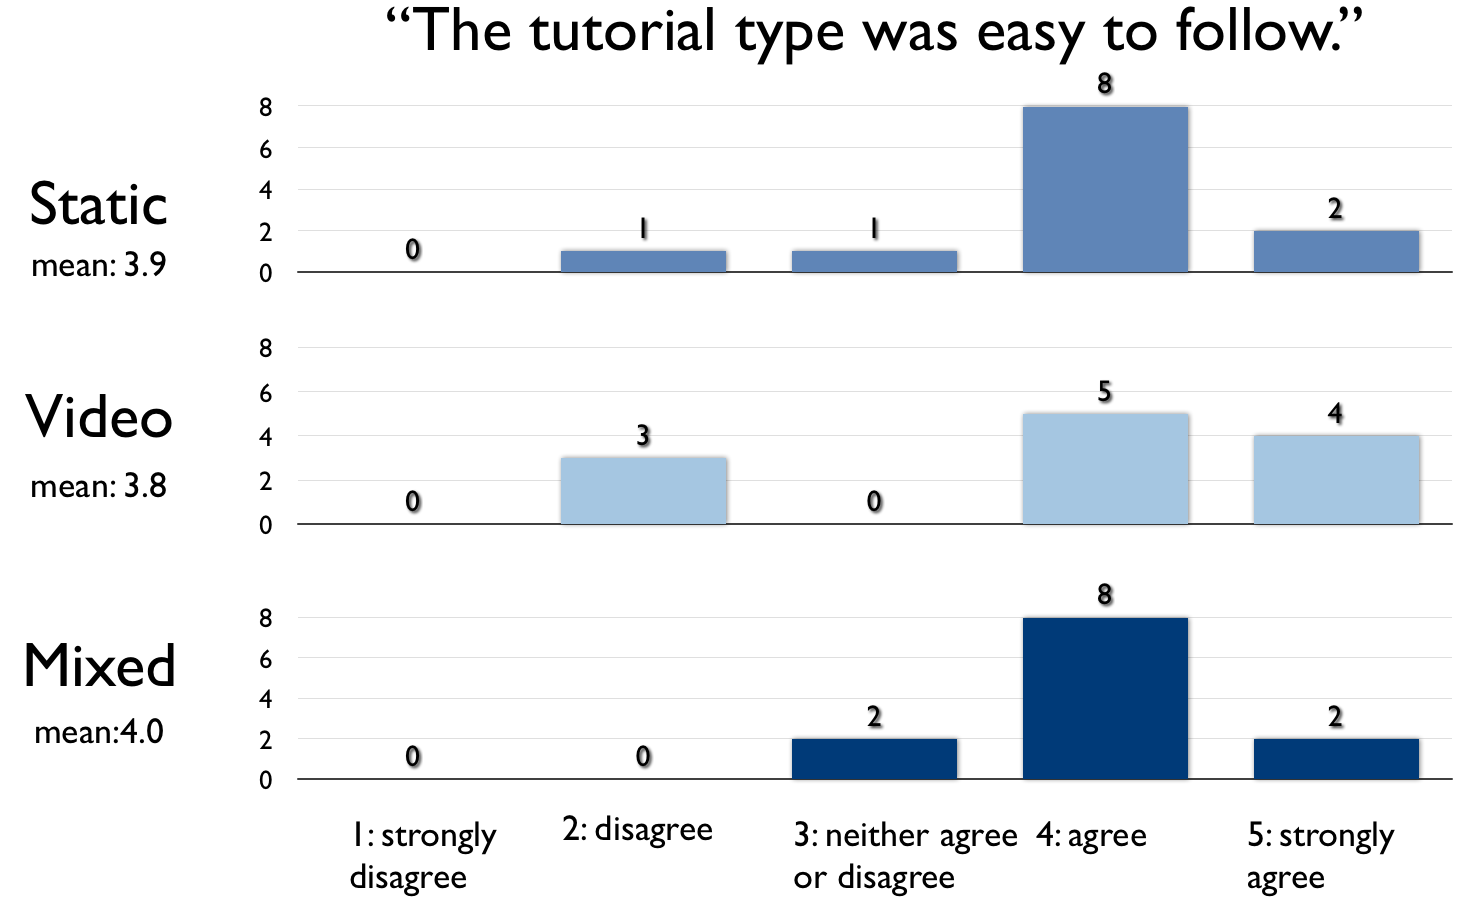
\includegraphics[width=\textwidth]{\demowiz/fig/results/likert}
  \caption{User feedback from questionnaire on the 7-point Likert scale.}
  \label{fig:demowiz_likert}
\end{figure*}

\subsubsection{Visualization as a Supportive Cue}
Participants answered that they were able to understand DemoWiz visualization of input events (µ = 6.0) and found it supportive for their presentations (µ = 6.3). They also commented that the DemoWiz visualization supported the presentation in various aspects: \iquote{the visualization reminds of the order of the content} (P1), \iquote{Really liked the ability to know what was coming up} (P2), \iquote{It provides better insight of the progress of the video} (P6), and \iquote{viz gave me an idea about timing or something I was going to forget to say} (P9).

\subsubsection{Narration Timing}
We coded the 20 recordings of participants' final presentations to observe the timing of narration of each action in correspondence with the video content (11 key events for both tasks). With DemoWiz, participants tended to \textit{anticipate} the upcoming events rather than talk afterwards, where the average timing was -0.1 seconds with DemoWiz (i.e., narrated the action before it happened) and 0.4 seconds with the Baseline condition (i.e., explained the action after it was shown). We found a significant difference in the number of times that events were anticipated by the narration, co-occurred, or occurred after the fact ($\chi $\textsuperscript{2}\textit{(2,220) = 8.6, p = .01}, see Figure~\ref{fig:demowiz_results_timing}).

In general, this supports our suspicion that DemoWiz would help in anticipating an event as opposed to talking about it after it occurred. More important though, was how often a narrator spoke about an event within several seconds of when the event actually occurred. By defining \textit{better} timing as when a presenter's explanation came within 2 seconds of a shown event (either prior, exact, or after), there was marginal significance by condition (\textit{p} = .089 with DemoWiz performing better). In addition, with the Baseline condition, the timing of narration was less consistent and off more, varying from 6 seconds early or 10 seconds late with a variance of 3.9 seconds, in comparison to the DemoWiz condition with at most 3 seconds early to 3 seconds late and a variance of 1.9 seconds.

Five participants had an obvious \textit{error} (forgot the next action or incorrectly narrated another action), had a long \textit{break} (waiting for more than 2 seconds until the action was made), or \textit{missed} an action (did not explain an important feature) when presenting with the Baseline condition. On the other hand, in the DemoWiz condition no errors were made, and there were only one long break and one miss from two different participants, respectively.

Participants' comments also support the fact that DemoWiz helped presenters anticipate the upcoming events. P7 explained, \iquote{(I) felt better able to time my speech to coincide with visual events, rather than trailing after them. Without the event visualizations, I felt like I was talking about what the audience had just seen, rather than having my words and visuals combine to a single message.}

\begin{figure*}[t]
  \centering
  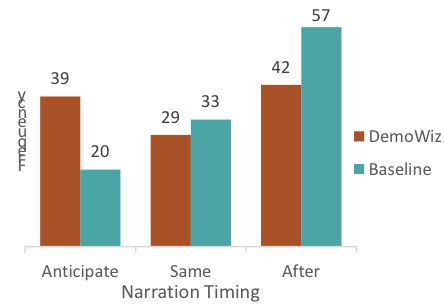
\includegraphics[width=\textwidth]{\demowiz/fig/results_timing}
  \caption{The number of times events were anticipated by the narration, co-occurred, or occurred after the fact.}
  \label{fig:demowiz_results_timing}
\end{figure*}

\subsubsection{Editing Experience}
We collected comments on the workflow. Participants found it easy to record (µ = 6.4) their demonstrations with DemoWiz. For editing features, they found it easy to edit in general (6.6), including controlling the playback speed (6.5) and adding pauses and stops (6.5), but it was less easy to add text notes (4.8); only two participants used this as reminders.

Although using different strategies, all of the participants adjusted the playback speed for matching their narration. Some sped up whenever possible and added stop markers for transitions; some slowed down the repetitive actions (such as drags) to demonstrate effects. P6 said, \iquote{I really liked being able to add ‘stop' events so I could \'fake\' my demo better.} DemoWiz made it easy for participants to separate the capturing and presentation preparation as P5 explained, \iquote{Overall, recording was very easy. In fact, as I got to the second task, I realized that I really don't need to think about the words as I record because later on I will be able to slow down and speed up time ...}

On average, the length of demo videos was 2'09\" before editing and 2'05\" after editing, and the presentation was 2'38\" long. Each participant spent 7.5 minutes on average to edit. For each demo of 44 segments on average, participants adjusted 3.15 segments for speedup and 4.25 segments for slowdown, and added 0.55 pause markers. In the DemoWiz condition, 1.2 stop markers and 0.2 text notes were added.

%!TEX root = ../thesis.tex
\chapter{Discussion}
\label{chapter_conclusion}

\section{Restatement of Contributions}
In this dissertation,

% How to design tutorial systems appropriately for different situations
% * level of expertise of instructor, learner
% * what are you trying to make easier?

\section{Remaining Challenges and Future Directions}

formal language
- now template, a set of techniques

\subsection{Collaborative Authoring}
a team, beyond a single author for larger projects or tasks

\subsection{Non-Linear Tutorials}
branching

\subsection{Mobile Capturing devices}
Tango, Structure Sensor, Leap Motion

\subsection{Emerging Instructional Space}

Augmented and virtual reality systems are becoming available to end users via affordable forms. However, designing AR and VR experiences extremely requires expertise and efforts. As devices offer personalized effects supported by sensing and input techniques, we need new authoring tools that focus on delivering story-centric experiences. Tools should also enable both professionals and amateurs to create and iterate designs efficiently in an immersive 3D world. ...research what future AR and VR creation tools would look like with new authoring processes.

by demonstration
``Microsoft HoloLens with Autodesk MotionBuilder'' by Jasper Brekelmans, \url{https://www.youtube.com/watch?v=yfl7pwXftUs}, licensed under CC BY 2.0


\begin{figure*}[ht!]
  \centering
\begin{tabular}{cc}
  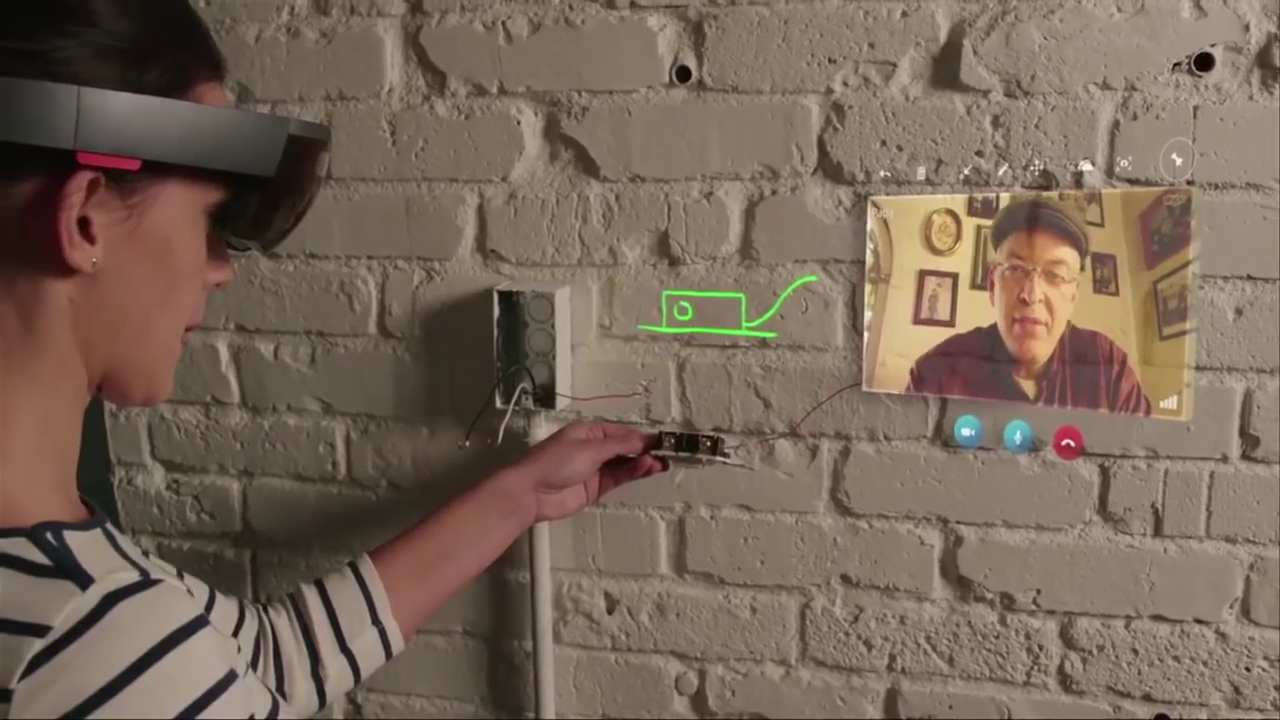
\includegraphics[width=0.4\textwidth]{\conclusion/fig/ar/hololens_fix1} &
  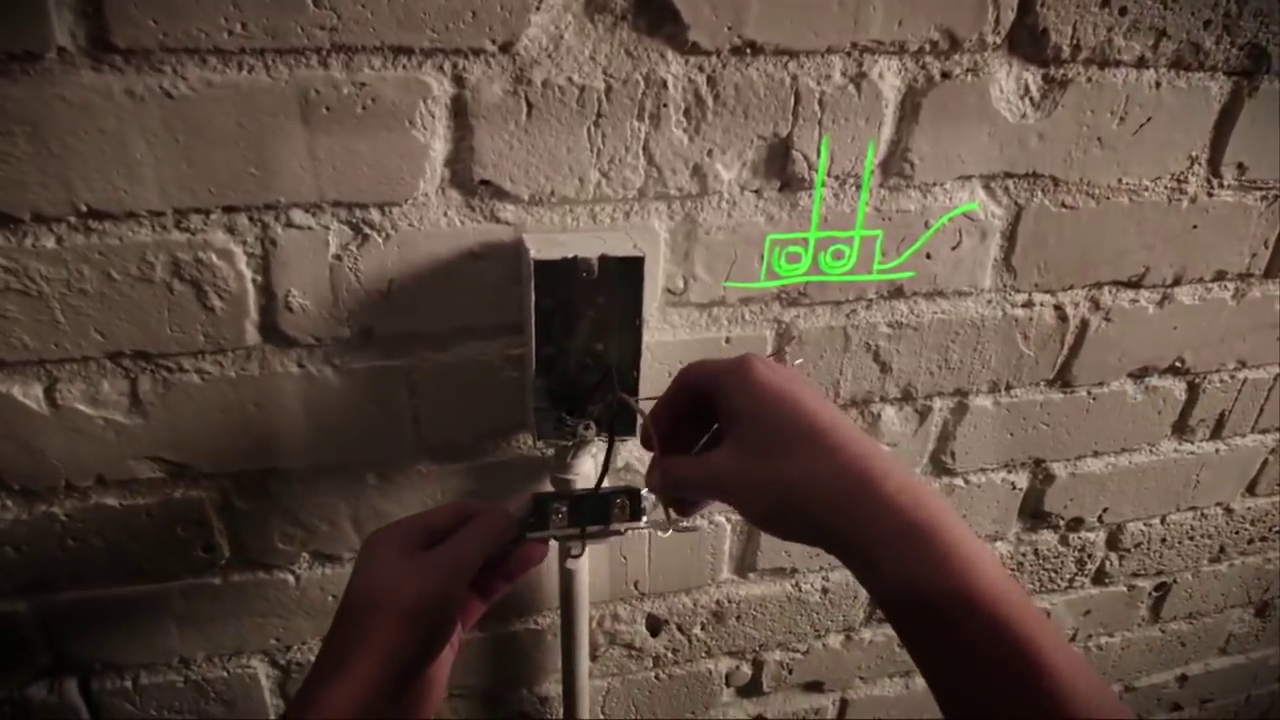
\includegraphics[width=0.4\textwidth]{\conclusion/fig/ar/hololens_fix2} \\
\multicolumn{2}{c}{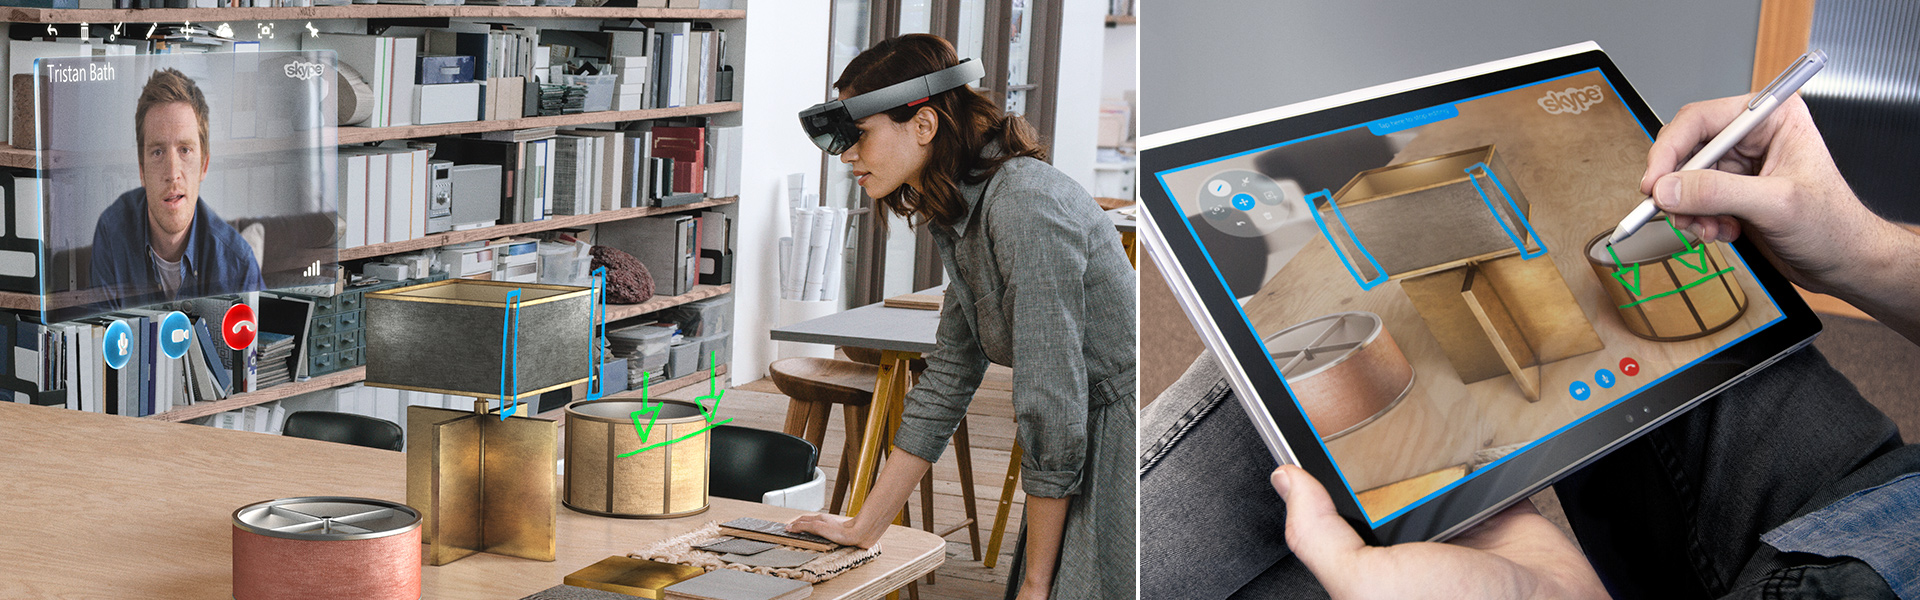
\includegraphics[width=0.82\textwidth]{\conclusion/fig/ar/hololens_skype} }
\end{tabular}
\caption{
  Microsoft's HoloLens~\cite{MicrosoftHoloLensSkype} has introduced an Augmented Reality application on providing real-time physical instructions from a remote instructor.
}
\end{figure*}

\section{Conclusion}
In this dissertation, we present video-based approaches designed for amateur users to produce and consume effective instructions from demonstrations. Using video and audio analysis techniques, our tools support recording, editing, and playback in a tutorial production process. We demonstrate results of our computer-generated tutorials from several domains, including software applications and physical activities. Our goal is to increase the quality of instructions created by tutorial authors and to support learners navigating and following the tutorials.


%!TEX root = ../thesis.tex
\chapter{DemoWiz: Visualization for Software Demonstration}
\label{chapter_demowiz}
% \chapter{DemoWiz: Re-Performing Software Demonstrations for a Live Presentation}

Showing a live software demonstration during a talk can be engaging, but it is often not easy: presenters may struggle with (or worry about) unexpected software crashes and encounter issues such as mismatched screen resolutions or faulty network connectivity. Furthermore, it can be difficult to recall the steps to show while talking and operating the system all at the same time. An alternative is to present with pre-recorded screencast videos. It is, however, challenging to precisely match the narration to the video when using existing video players.

In this chapter, we introduce DemoWiz\footnote{This work was published at CHI 2014~\cite{Chi:2014:DRS:2556288.2557254}.}, a video presentation system that provides an increased awareness of upcoming actions through glanceable visualizations. DemoWiz supports better control of timing by overlaying visual cues and enabling lightweight editing. A user study shows that our design significantly improves the presenters’ perceived ease of narration and timing compared to a system without visualizations that was similar to a standard playback control. Furthermore, nine (out of ten) participants preferred DemoWiz over the standard playback control with the last expressing no preference.

%!TEX root = ../thesis.tex
\chapter{Introduction}
\label{chapter_introduction}

When attempting to accomplish unfamiliar, complicated tasks, people often look for tutorials to follow instructions. From performing daily tasks such as cooking and operating a machine, using software applications, to physical activities like sports and dance performance, each domain involves specific ``how-to'' knowledge with a certain degree of complexity~\cite{ryle1945knowhow}.
%
Instructions, which describe how a specific goal can be accomplished, are a tool for people to self-learn a task~\cite{Smith03iimanufacturer}. Studies have shown that visual instructions are cognitively favorable by people as they are easier to comprehend and remember than text information~\cite{Harrison:1995uh,mayer1996less,Heiser:2004:IVC:989863.989917}. In history, pictorial instructions have been created from the Middle Age to explain dancing or weapon operations~\cite{mijksenaar1999open}. It was found that the first use of letters in technical drawing for text referral was by Italian polymath Leonardo da Vinci. In 1737, French engineer de B{\'e}lidor~\cite{de1737architecture}'s diagrams were the first to apply arrows to indicate direction of movements (see Figure~\ref{fig:intro_arrows}).
%
From 1760, when the Industrial Revolution introduced mass production, instructions have been seen widely for various products and uses.

\begin{figure*}[h!]
  \centering
  \begin{minipage}{\textwidth}
  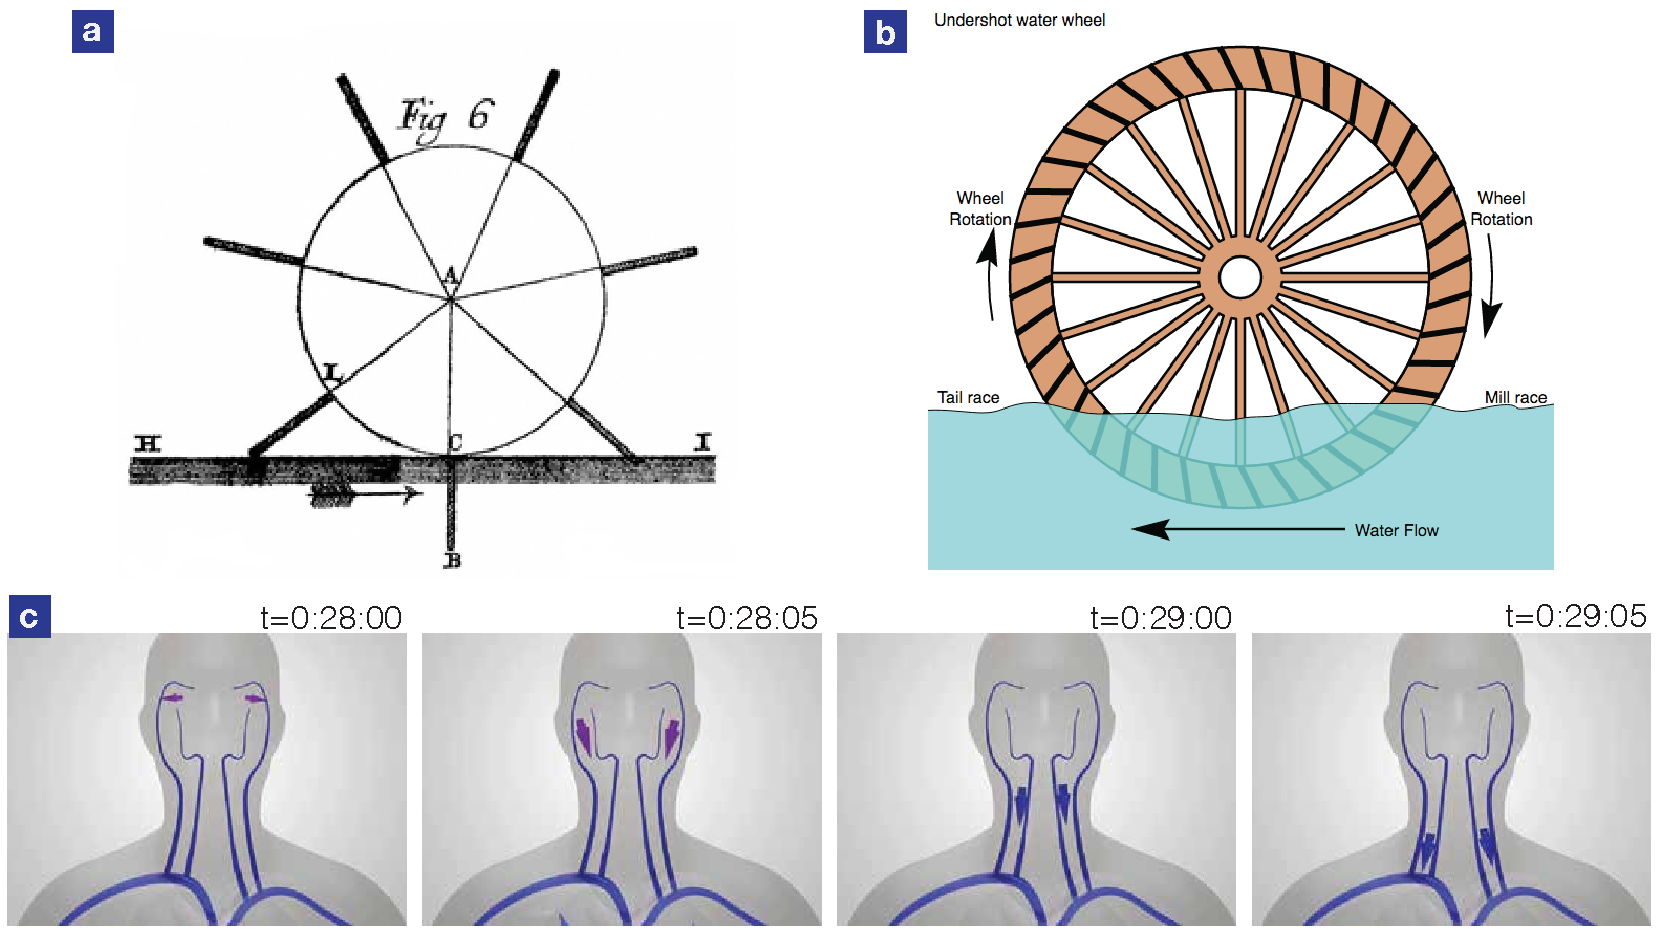
\includegraphics[width=\textwidth]{\intro/fig/arrows/arrows}
  \caption[Uses of motions arrows in visual instructions.]{Uses of motions arrows in visual instructions:
  %
  a) Year 1737: The first use of a motion arrow in an illustration explains the impact of water flow of a water wheel~\cite{de1737architecture},
  % http://www.buw-output-archiv.uni-wuppertal.de/ausgabe1/steinle/index-en.html
  %
  b) Year 2002: Similarly, arrows are used to explain the water flow and rotation of an undershot water wheel\footnote[1]{Original artwork by Daniel M. Short, ``Schematic diagram of an undershot water wheel'', licensed under CC BY-SA 2.5},
  % https://en.wikipedia.org/wiki/File:Undershot_water_wheel_schematic.svg
  %
  c) Year 2014: An animation visualizes the blood flow using motion arrows\footnote[2]{Video by Bioscience Credentials, ``Blood Flow in the Human Body'', \url{https://youtu.be/GwX41xm9esY}, licensed under CC BY 3.0}.
  }
  \label{fig:intro_arrows}
  \end{minipage}
\end{figure*}

Since the late 1990s, the advance in computer technologies has introduced more versatile instructional design. Instructions can now be created via software tools rather than hand drawing; they can include multimedia such as images and videos in several forms; they can be accessed through the Internet, as well as in hard copy.
%  the general purpose computers and the Internet
%
This advancement also enables consumers or end-users to document and share their domain knowledge~\cite{Lafreniere:2012tl}. As of today, popular tutorial sharing sites like Instructables has over 220,000 articles~\cite{InstructablesProjects}, wikiHow provides over 192,000 articles~\cite{wikiHowStatistics}, Food.com serves over 500,000 user-generated recipes with 125,000 photos~\cite{FoodComAbout}, and YouTube hosts over 285 million How-To videos\footnote{YouTube, \url{https://www.youtube.com/}, accessed June 2016}.
%
The variety of topics, content, and presentation styles provides learners more options to understand domain knowledge.
%
However, navigating a tutorial using existing tools remains inefficient for following step-by-step instructions. It can be challenging to observe details from text and images or find specific piece of information in a video through a timeline with conventional video players.
%
On the other hand, producing high-quality instructions that are easy to follow requires authoring expertise and a significant time investment. It involves several stages to design, record, and edit multimedia materials of a task using a variety of creation tools~\cite{Torrey:2007he,Tseng:2014:PVP:2598510.2598540,Muller:2009tw}.\\

The goal of this dissertation is to investigate interactive instructional design and develop computational tools that support the authoring process.
%
To contribute to computational methods of authoring user-generated instructions, two research questions that this work focuses on are:

\begin{itemize}
  \item How can authoring tools support domain experts in efficiently creating effective, high-quality instructions based on video-recorded demonstrations?
  \item How can new tutorial formats help authors better express their intent and help learners understand and follow the author's instructions?
\end{itemize}

This dissertation presents video-based computational approaches that enhance tutorial creation and consumption from author demonstrations.
We encode the current practices from professional authors into automatic algorithms and interactive techniques.
Our goal is to dramatically increase the quality of amateur-produced video instructions, which in turn improves learning for viewers who interactively navigate the content.
%
We will introduce five interactive systems that we develop to address these challenges. These tools cover both software applications (e.g., image manipulation tasks or browser navigation) and physical activities (e.g., Do-It-Yourself projects or dance movements) for recording, editing, and replaying instructional content.

% ---------------------------------------------------------------

\section{Challenges of Creating and Consuming Instructions}

Visual instructions are the dominant form of instructional design~\cite{mijksenaar1999open}. Cognitive load theory of multimedia learning suggests that learners process information using distinct channels, one for visual and the other for verbal formats~\cite{sweller1998cognitive,sweller1988cognitive,paas2003cognitive}. It was found that learners performed better when received a pictorial summary of a scientific system than those who received the full text alone or the full text with the summary~\cite{mayer1996less}.

Among all the multimedia support, videos are a common form to present instructions. We suspect that the great popularity of videos is due to the following reasons:
%
First, consumer devices and software have become affordable for authors to quickly record activities and later share via online platforms at minimum cost.
%
% ** describe the difficulties of making knowledge "explicit", esp. for actions and motions
Second, videos can be an efficient medium to document activities. Transferring know-how concisely and effectively to the audience is challenging. It especially requires efforts when a task involves \emph{tacit knowledge}, which is a kind of knowledge that is difficult to articulate in a written or verbal form~\cite{polanyi1958personal, Klemmer:2006:BMF:1142405.1142429}. Examples of tacit knowledge include dancing, riding a bike, or driving nails with a hammer. Dancers can perform movements fluently with music. If they are asked to focus on the composite pieces, such as the arm and foot actions or rhythm, they might get confused and fail to express the entire movement~\cite{polanyi1958personal}. Very often, recording a video eases the difficulties of describing the entire activities in an explicit form.
%
This leads to another motivation that videos also provide an effective channel to convey ideas with adequate amounts of details. Learners can visually observe the exact actions in a video as if an expert were coaching in person~\cite{Kuznetsov:2010:REA:1868914.1868950}.

However, while videos are easy to produce, they can include a lot of unnecessary footage. Inevitable content such as pauses, mistakes, and long repetitive actions makes it difficult for learners to focus on the most important steps and actions. A lot of authoring effort commonly goes into extracting footage, applying visual effects, and adding subtitles and annotations.
%
In addition, even with a well-edited video, navigating using a conventional video player remains inefficient. Learners with various needs could have a hard time skimming to an interesting moment or perceiving high-level overviews. Alternatively, a pictorial summary or static step-by-step tutorials presented with text and images can effectively guide knowledgeable learners through familiar tasks.

% The goal of this dissertation to develop video-based recording, editing, and playback tools are optimized for creating and consuming instructional demonstrations. I combine the advantage of ubiquitous video recording with the benefits of video and structured tutorial formats. I aim to dramatically increase the quality of amateur-produced video instructions, which in turn improves learning for viewers who interactively navigate the content.

% ----- MixT ----- %

\subsection{New Tutorial Formats}

Both static and video tutorials have strengths, but neither format alone is well suited for all learning needs that learners may have.
%
To combine the benefits, we design a new instructional presentation called \emph{MixT} (mixed-media tutorials) that improves learners' success in following instructions (see Figure~\ref{fig:mixt_intro}).
%
MixT presents step-by-step static instructions and includes in-place video clips for each operation.
%
With MixT, learners can quickly scan forward and backward on a web page to obtain an overview of a task. Embedded videos help them understand continuous, complex manipulation, such as brushing on a canvas and adjusting control points.
%
MixT's playback UI allows learners to interactively control \emph{when} to see images or videos, and \emph{how} to render videos.
%
Video editing techniques are applied to emphasize instructions, including cropping salient screen regions and highlighting interaction.
%
In our within-subject experiment, MixT successfully reduced numbers of errors and attempts made by learners when following image manipulation tasks.
% To demonstrate , MixT captures screencast video and operation events of a software demonstration.

\begin{figure*}[t]
  \centering
  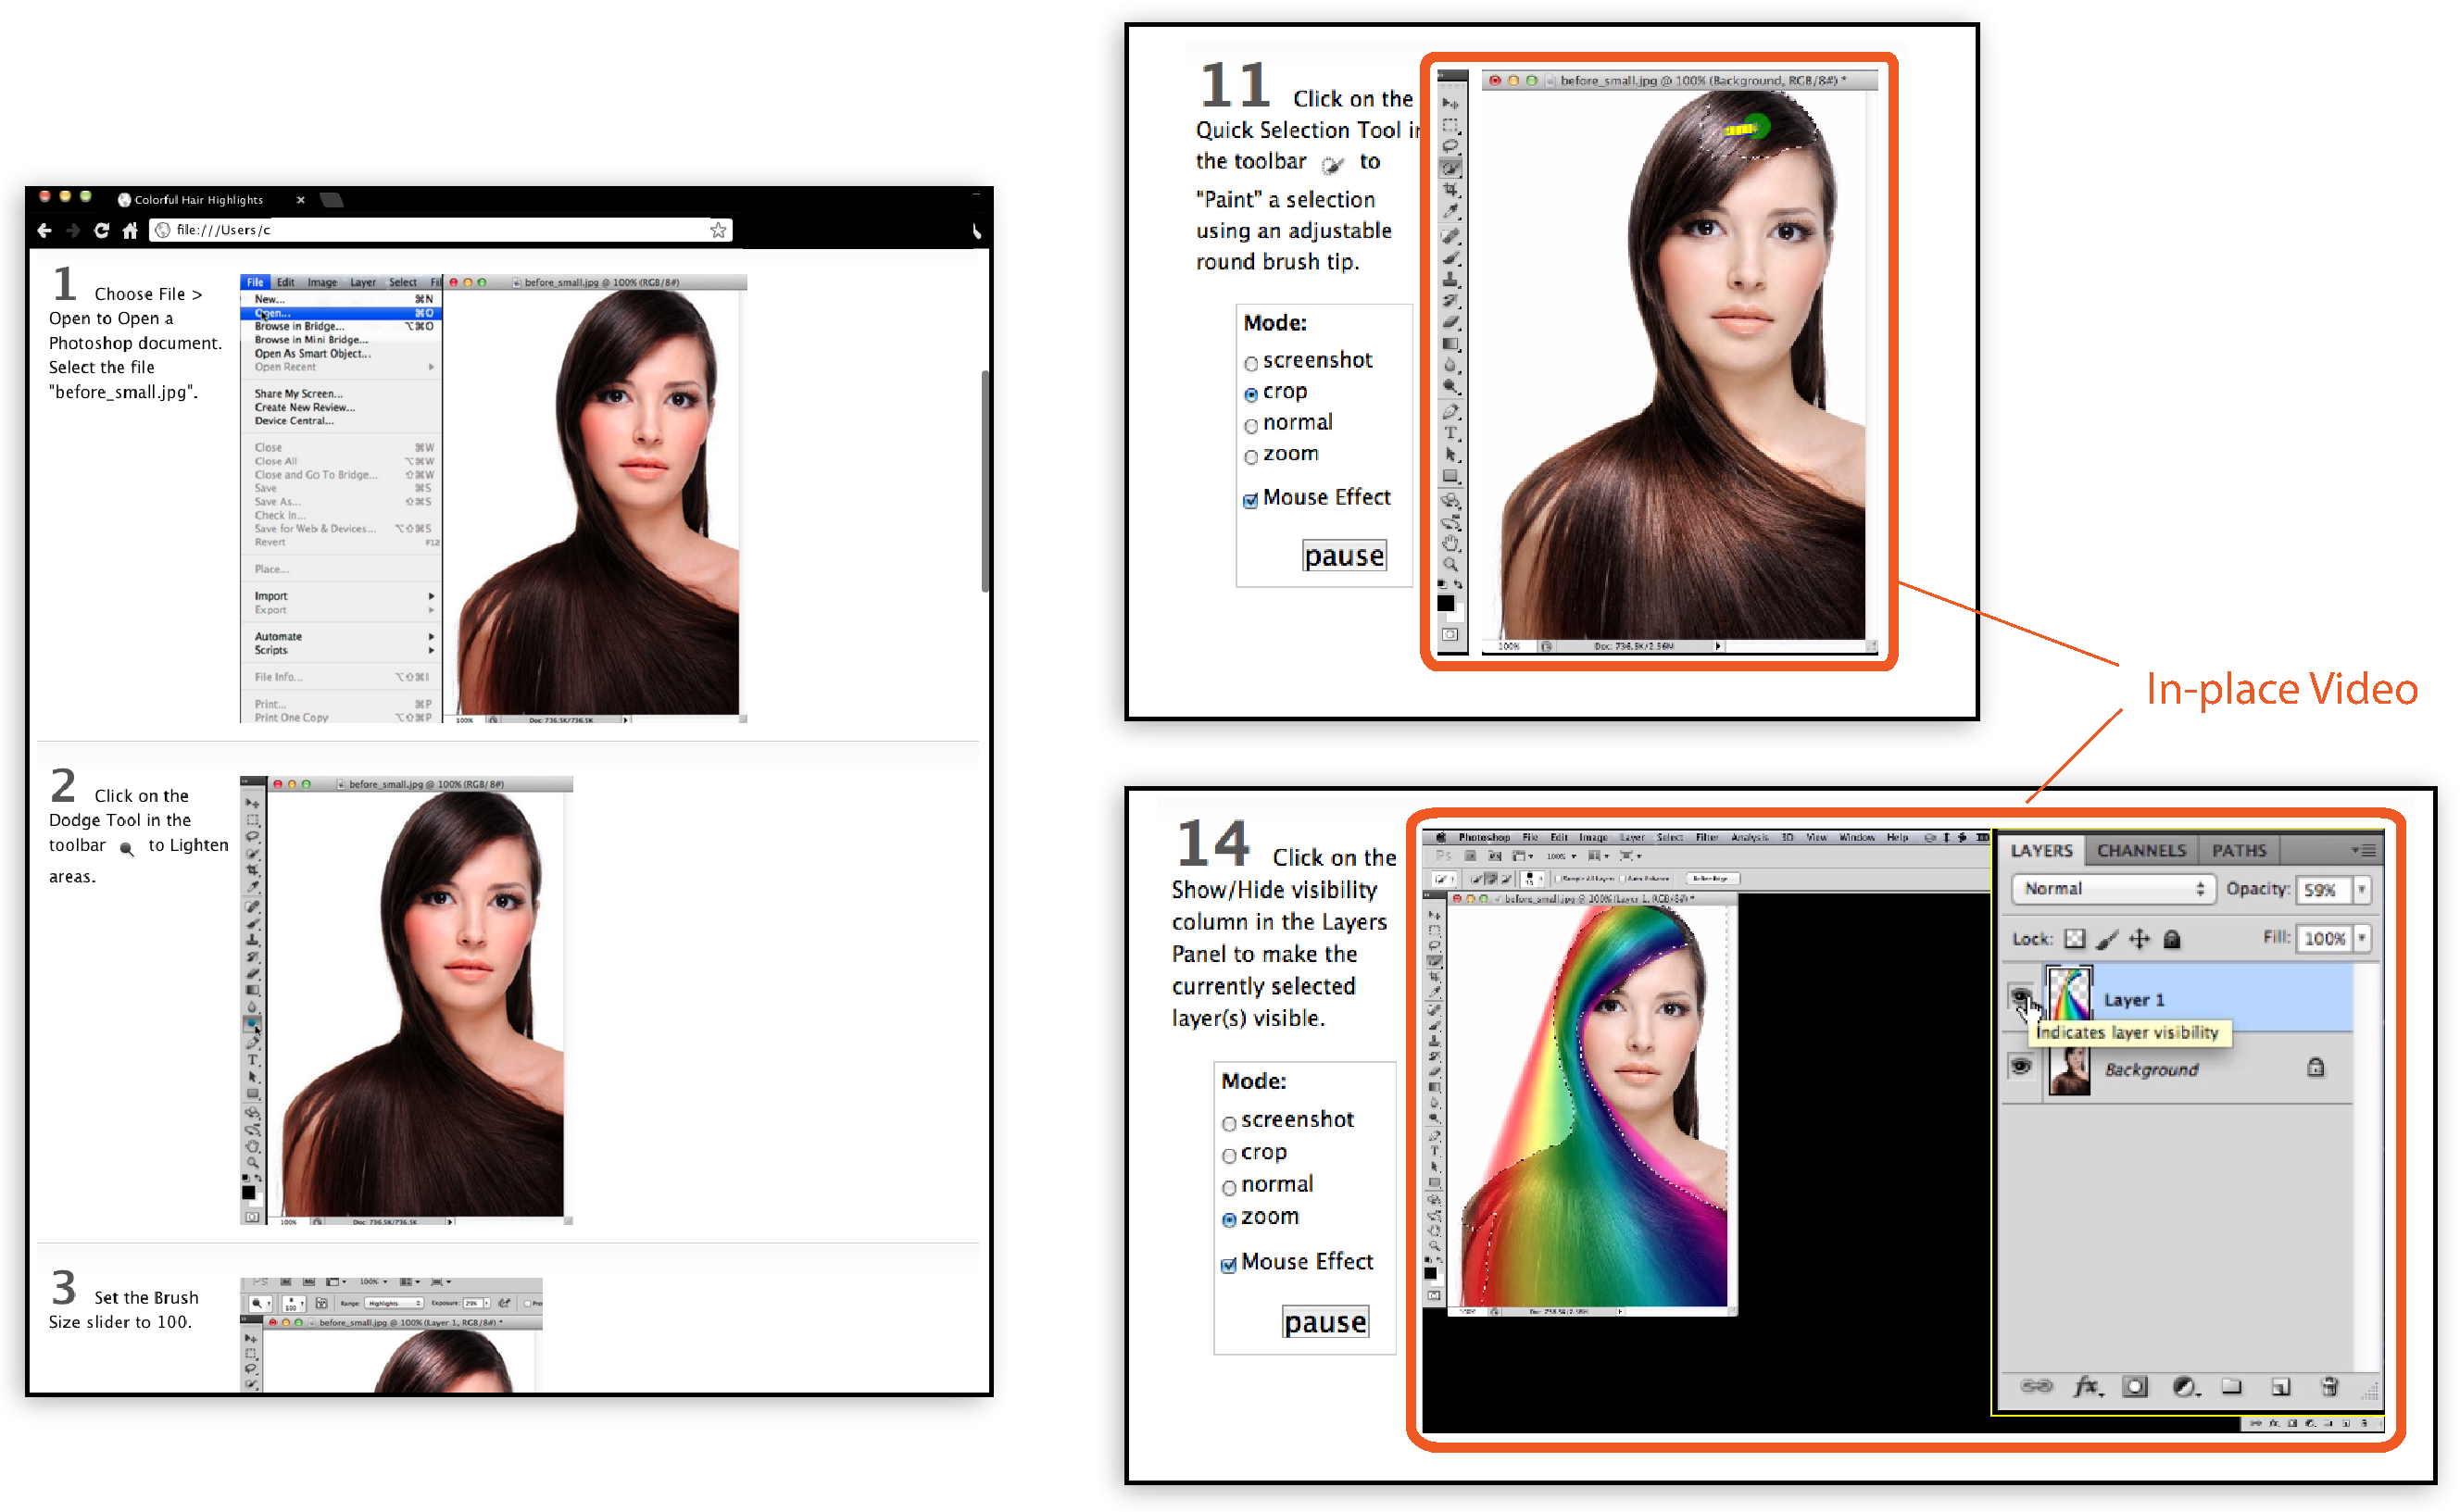
\includegraphics[width=0.8\textwidth]{\intro/fig/mixt_intro}
  \caption{MixT generates step-by-step tutorials (left) that contain static and video information from task demonstrations. Videos are automatically edited and offer different views (right) to highlight the most relevant screen areas for a step. Visualizing mouse movement helps learners understand a complex action.}
  \label{fig:mixt_intro}
\end{figure*}

% ----- DemoWiz ----- %
MixT offers a novel way of navigating instructional content with a combination of static step-by-step and embedded video presentations. If an author wants to narrate over a video recording to illustrate a demo, it can be challenging to pace oneself at the suitable timing without expecting \emph{when} and \emph{what} action is taking while a video is playing.
%
We design \emph{DemoWiz}, a system that augments a screencast video with visualizations (Figure~\ref{fig:demowiz_intro}). By logging the input events of a software demonstration, DemoWiz overlays glyphs to visually guide viewers to the next action along with the time remaining before the action occurs. This enables viewers to anticipate the video content rather than react to it.
%
Our study showed that fewer anticipation errors and narration delays were made with DemoWiz.

\begin{figure*}[t]
\centering
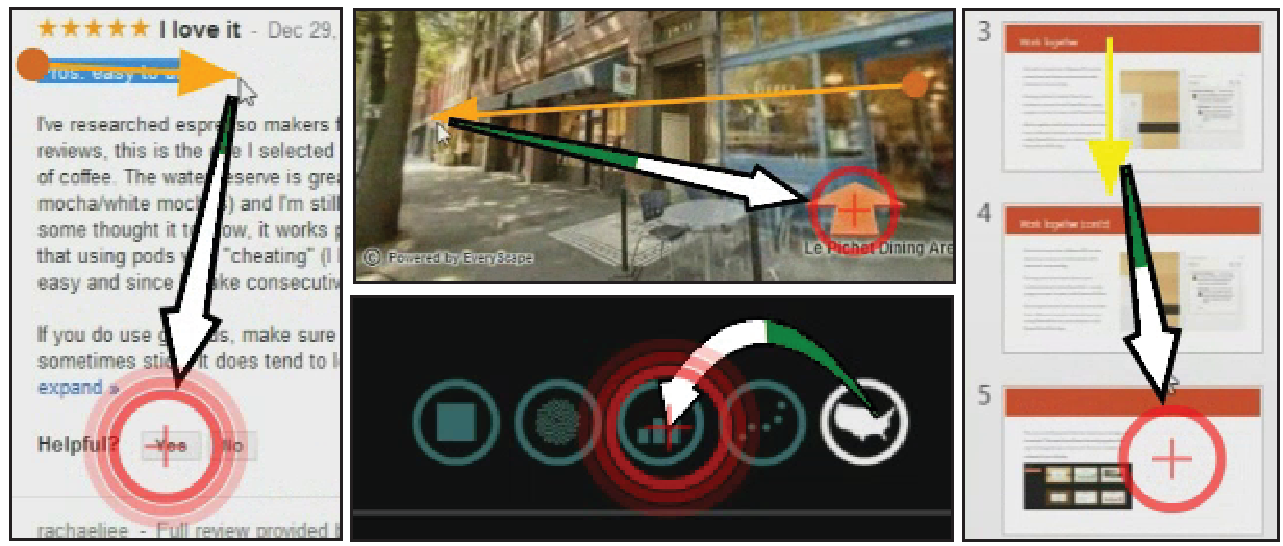
\includegraphics[width=0.7\columnwidth]{\intro/fig/DemoWiz}
\caption{DemoWiz visualizes input events in a screencast video to help viewers anticipate the upcoming event for following a software demonstration.}
\label{fig:demowiz_intro}
\end{figure*}

\subsection{Tutorial Generation from Software Demonstration}

While new tutorial formats are shown to be useful, manually creating instructions can be extremely time- and effort-consuming. In response, we design computational methods to automate the creation process from an author demonstration. MixT and DemoWiz capture screencast video and input device events from a demonstration of a task in a software application. MixT also records application commands for video analysis. Computer vision and visualization techniques are integrated to segment a video into steps, extract salient information, and add visual highlights.
%
In addition, DemoWiz supports an editing phase where authors can adjust the timing of events in a video. Playback speed of recorded actions can be modified or skipped via an editing UI. Our studies showed that our algorithms for step segmentation, event detection, and visualization were effective (\textless8\% error rate in MixT and 0\% in DemoWiz).

\subsection{Interactive Tutorial Authoring from Physical Demonstration}

% ----- DemoCut ----- %

Moving beyond software applications, support for authoring instructions of tasks that take place in the physical world is lacking. Activity recognition remains an open research question, and making authoring decisions during a demonstration can be difficult.
%
To address this problem, we first look into Do it yourself (DIY) project tutorials, which help people learn knowledge and skills to complete a task independently.
%
We developed \emph{DemoCut}, a semi-automatic video editing system that improves the quality of amateur instructional videos for physical tasks (Figure~\ref{fig:democut_intro}). DemoCut asks authors to describe key ``moments'' in a recorded demonstration video using a set of markers. Based on the annotations, our system analyzes the audio and visual activities to automatically organize the video into meaningful segments. Editing decisions are applied to support both \emph{temporal effects} that increase playback speed or skip segments, as well as \emph{visual effects}, such as zooming, subtitles, and visual highlights. A playback interface allows authors to quickly review and edit the automatically generated effects.
%
Our studies showed that video tutorials created by DemoCut in five DIY domains were concise in terms of video length and descriptive instructions with low effect error rates.

\begin{figure*}[t]
  \centering
  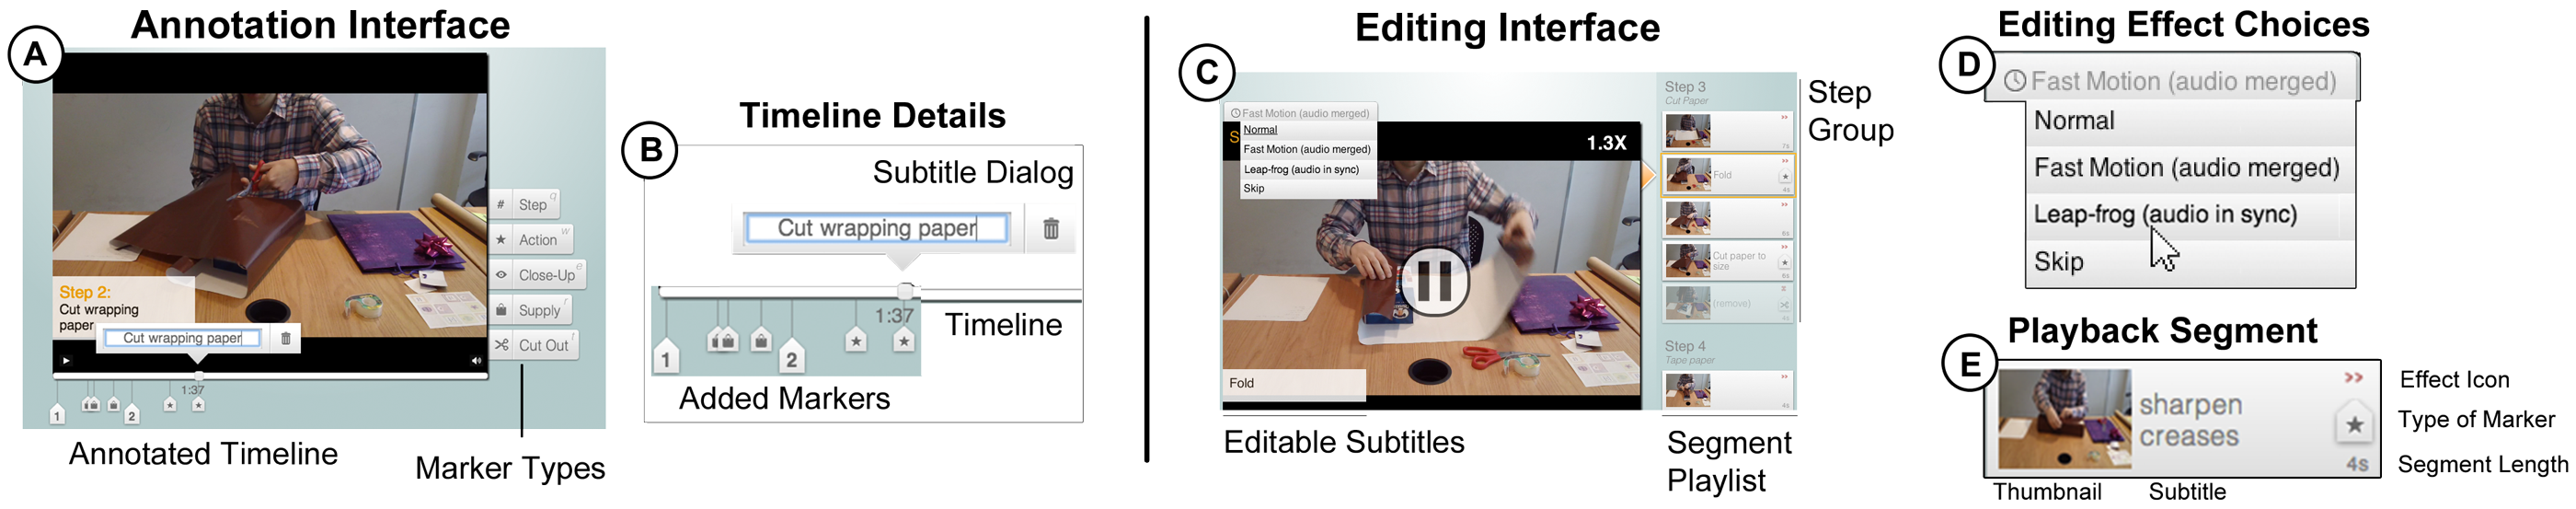
\includegraphics[width=\textwidth]{\intro/fig/DemoCut}
  \caption{DemoCut asks authors to mark key moments in a recorded video of demonstration using a set of marker types. Based on marker information, the system uses audio and video analysis to automatically organize the video into meaningful segments and apply appropriate video editing effects, which can be modified via a playback UI.}
  \label{fig:democut_intro}
\end{figure*}

% ----- Kinectograph ----- %
Through the process of designing DemoCut for automatic DIY video editing, we observed that for tasks that require larger space and more movements, instructors often have to adjust the position and viewing angle of a camcorder. Some authors choose to set up multiple cameras and later select the best shot from video streams, while some invite another person who controls the camcorder during a demonstration.
%
To enable authors to record their demonstration without acquiring additional cameras or cameraman, we design \emph{Kinectograph}, a video recording device with a single camera that automatically tracks and follows specific body parts, e.g., hands, of an instructor in a video (see Figure~\ref{fig:kinectograph_intro}). It utilizes a Kinect depth sensor to track skeletal data and adjusts the camera angle via a 2D pan-tilt gimbal mount. Authors can freely move around in space to demonstrate a task and monitor real-time video preview through a tablet application.

\begin{figure}[!t]
  \centering
  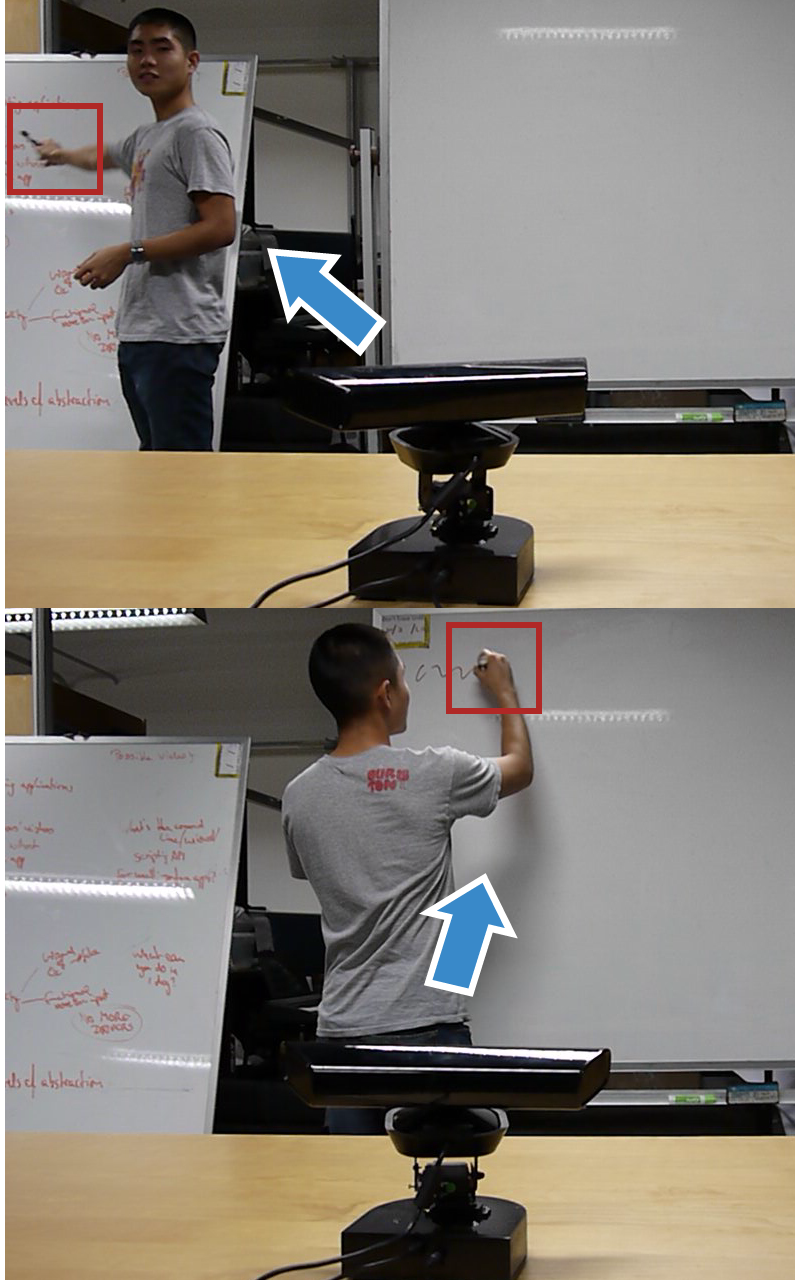
\includegraphics[width=0.65\columnwidth]{\intro/fig/Kinectograph}
  \caption{Composed of a Kinect camera to track author movement and a motorized dock to pan and tilt the camera, Kinectograph allows the author (or their hand) remains centered in the recorded video in real-time.}
\label{fig:kinectograph_intro}
\end{figure}

% ----- DemoDraw ----- %

The successful experiences supporting motion-based recordings motivated me to apply our demonstration-based approach to a domain that is entirely driven by movements. In sports, dance performance, and body gesture interfaces, movement instructions are often conveyed with drawings of the human body annotated with arrows or stroboscopic effects~\cite{cutting_representing_2002}. However, current practices require authors to manually sketch or trace subjects from photographs, which is time-consuming and difficult to make changes once created.
%
We design \emph{DemoDraw}, a system that generates concise illustrations from author demonstration (see Figure~\ref{fig:demodraw_intro}). With DemoDraw, an author records one or more motions by physically demonstrating in front of a Kinect sensor. In a multi-modal Demonstration Interface, DemoDraw segments speech and 3D joint motion into a sequence of motion segments, each characterized by a key pose and salient joint trajectories. Based on this sequence, a series of illustrations is automatically generated using a stylistically rendered 3D avatar annotated with arrows to convey movements. Once a suitable sequence of steps has been created, a Refinement Interface enables fine control of visualization parameters.
%
In a three-part evaluation, our results show 4 to 7-step illustrations can be efficiently created in 5 or 10 minutes on average.

\begin{figure}[t]
  \centering
  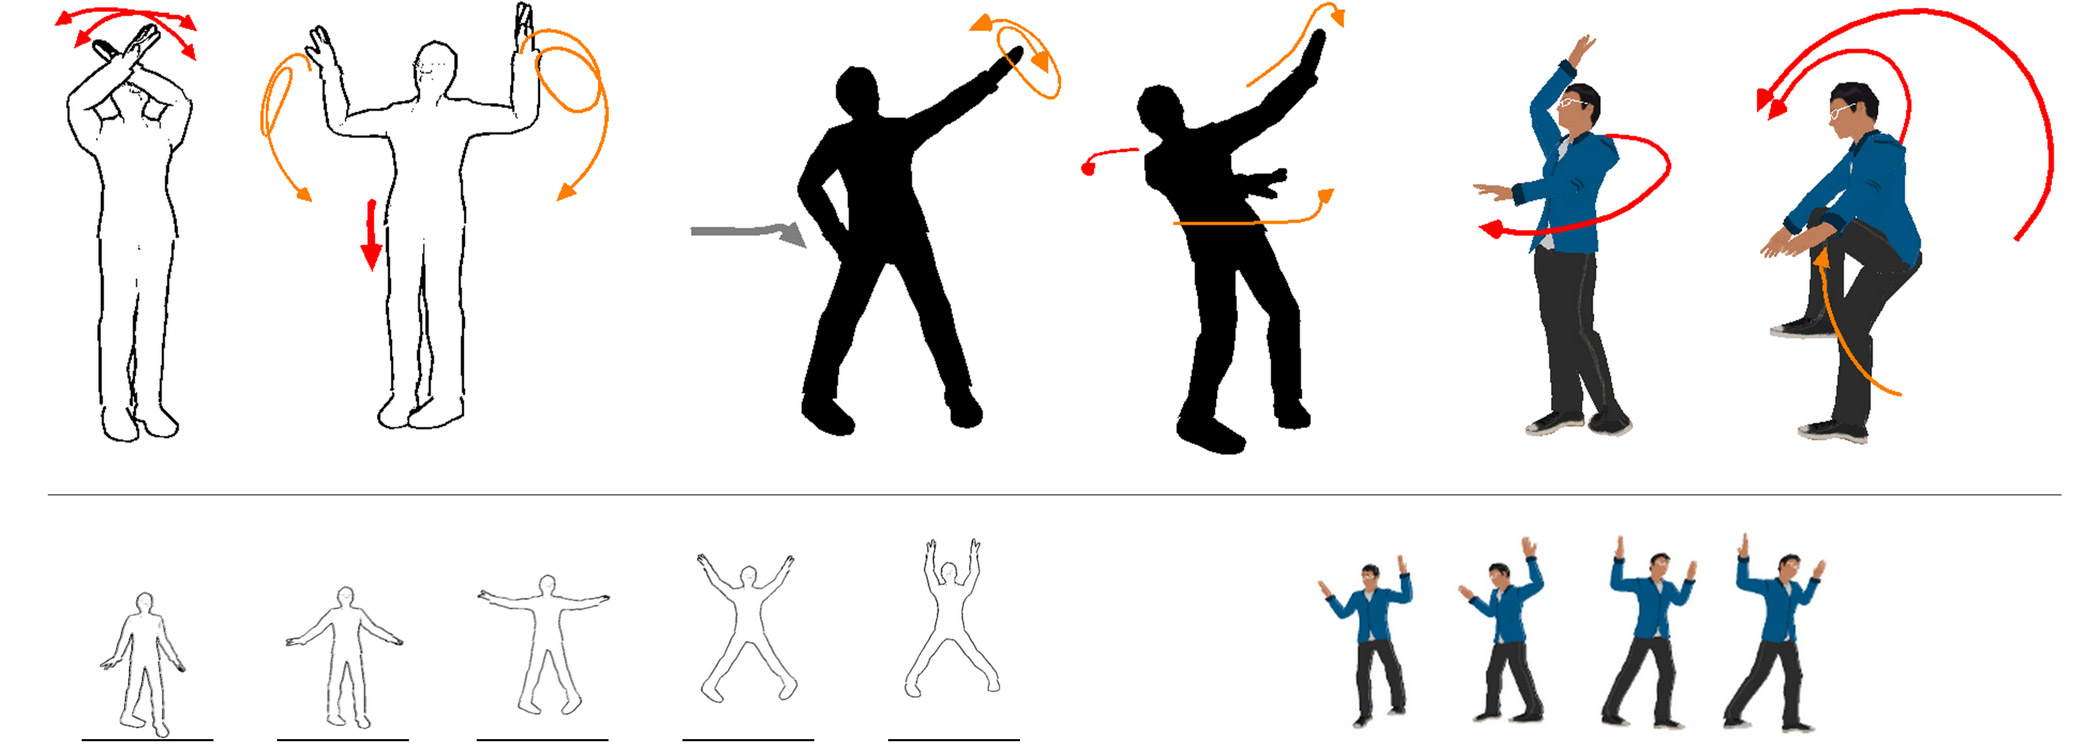
\includegraphics[width=\columnwidth]{\intro/fig/DemoDraw}
  \caption{DemoDraw's multi-modal approach enables authors to capture motion, verify results, and re-perform portions if needed to generate step-by-step motion illustrations.}
  \label{fig:demodraw_intro}
\end{figure}

% ---------------------------------------------------------------

\section{Thesis Contributions}

Overall, our video-based approaches consider key events or moments that are important to a learner. This information can be derived from software event logs or human annotation of physical tasks when automatic recognition remains challenging. Based on the metadata and video streams, we propose automatic methods to generate concise instructions for two task domains, software applications and physical tasks (see Figure~\ref{fig:space}). Our approaches support authors from recording demonstrations to editing and reviewing system-generated instructions. Interactive controls are available in different stages via desktop or multi-modal interfaces.
%
We demonstrate a series of systems that consider production stages of tutorial creation and learning. We present the rationale and technical challenges of these interactive system designs. Each system is evaluated both quantitatively and qualitatively to study the usability in authoring and learning.

\clearpage
The contributions of this dissertation include:

\begin{itemize}
\item New instructional formats that consider the learning needs from several domains, including software applications and physical activities.
\item Multi-modal interaction techniques for novice or amateur authors to create effective instructions by demonstration.
\item Automatic or semi-automatic approaches using video and audio analysis that includes authors in the loop to produce high-quality instructions.
\end{itemize}

\begin{figure}[t!]
  \centering
  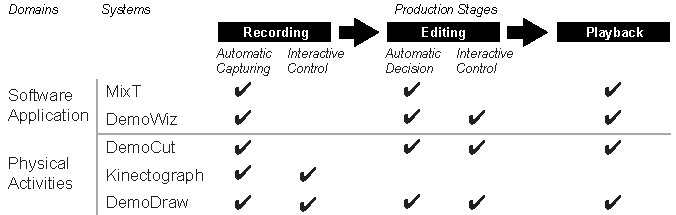
\includegraphics[width=0.9\columnwidth]{\intro/fig/space}
  \caption{A design space of the creation and consumption process for tutorials. It involves three phases of recording, editing, and playback in either software domain or a physical world. This dissertation proposes a series of systems that focus on various aspects in this design space.}
  \label{fig:space}
\end{figure}

% ---------------------------------------------------------------

\section{Overview}

The rest of this dissertation is structured as follows:
%
In Chapter \ref{chapter_background}, we define terminology used in instruction creation and consumption process based on literature. We review studies on why people rely on tutorials in general, how the formats of instructions matter, and the current practices of authoring instructions.
%
In Chapter \ref{chapter_related_work}, we review the literature on research and technologies used in supporting activities of authoring and consuming instructions.

We presented two systems that generate interactive tutorials for software applications.
% MixT
In Chapter \ref{chapter_mixt}, we present our study on how a new tutorial format supports learners in following step-by-step instructions with mixed media, including static text, images, and video clips. We introduce our creation tool called MixT, which automatically generates such new tutorial format from a software demonstration.
% DemoWiz
Chapter \ref{chapter_demowiz} introduces DemoWiz, a system that assists viewers in capturing the timing of input events in a screencast demo video. DemoWiz supports recording, editing, and reviewing stages in a production process with an authoring and playback UI.

Then, we introduced three systems designed for real-world tasks that involve physical demonstrations.
% DemoCut
In Chapter \ref{chapter_democut}, we present a semi-automatic tool for DIY video editing. Our system, called DemoCut, provides two authoring interfaces, annotation and editing, that enable authors to mark a demo video and review and modify the automatically edited results. The design is based on an fundamental understanding of DIY activities.
% Kinectograph
In Chapter \ref{chapter_kinectograph}, we focus on a recording device that automatically follows a demonstrator for filming instructional videos. The Kinectograph system tracks an author's position and body parts and provides an authoring interface for real-time camera control.
% DemoDraw
Finally, in Chapter \ref{chapter_demodraw}, we introduce a multi-modal approach for authors to generate motion illustrations by physically demonstrating the movements. DemoDraw is a system that segments speech and 3D joint motion into a sequence of motion segments and renders effective illustrations. Two authoring interfaces enable authors to navigate, re-perform, and edit visualization parameters.

% Conclusion
Throughout this dissertation, we discuss how our video-based approaches increase the quality of amateur-produced video instructions. Chapter \ref{chapter_conclusion} concludes our work on tutorial creation and consumption in both software and physical instructions. New directions for future research on interactive tutorials are proposed.

% ---------------------------------------------------------------

\section {Prior Publications}

This dissertation is based on papers published in previous ACM conference proceedings: the MixT system was published at UIST 2012~\cite{Chi:2012:MAG:2380116.2380130}, DemoWiz at CHI 2014~\cite{Chi:2014:DRS:2556288.2557254}, DemoCut at UIST 2013~\cite{Chi:2013:DGC:2501988.2502052}, and Kinectograph at CHI 2013~\cite{Cheng:2013:BCC:2468356.2468568}; DemoDraw will be published at UIST 2016~\cite{Chi:2016:DemoDraw}.

While I am primary author on all publications and led the described projects, this research could not have been completed without my advisor Bj\"orn Hartmann and my collaborators that I have been fortunately to work with. Specifically, Dr. Mira Dontcheva and Dr. Wilmot Li at Adobe Research provided valuable guidance on three projects (MixT, DemoCut, and DemoDraw); Dr. Steven M. Drucker and Dr. Bongshin Lee at Microsoft Research guided the DemoWiz project with their expertise on visualization; Professor Daniel Vogel at University of Waterloo greatly contributed to the DemoDraw project. A group of MS and undergrad students at UC Berkeley and Adobe contributed to implementation, design, and user study in the projects, including Sally Ahn and Amanda Ren in MixT, Joyce Liu and Jason Linder in DemoCut, and Derrick Cheng and Taeil Kwak in Kinectograph.

% We are all natural performers. Humans are proficient at demonstrating how to perform a task in action. However, articulating knowledge into a written or structured form can be extremely difficult. From dancing, repairing a machine, to operating software applications, it remains a challenge how everyday activities can be efficiently captured for a remote learner to understand.

%!TEX root = ../thesis.tex

\chapter{Related Work}
\label{chapter_related_work}

While existing practices require tutorial authors to create instructions manually, HCI and Computer Graphics communities have introduced novel technologies for authoring tutorials, including automatic generation methods and interactive editing tools.
%
In this chapter, I survey state-of-the-art techniques for generating instructions for both software applications (Section \ref{related_software}) and physical tasks (Section \ref{related_physical}).
%
Furthermore, existing instructions are mainly offered in the forms of conventional media, such as static tutorials (print-outs or web) or videos. With software systems, \keyword{interactive tutorials} have been introduced for learners to interactively review instructional content. I will discuss various forms of such kind of instructions by prior research, which leads to a discussion on the remaining gaps in tool support for creating and navigating instructional content.

% -------------------------------------------

\section{Instructions for Software Applications}
\label{related_software}

\subsection{Workflow Capturing and Tutorials}

Revealing operation history has shown to be effective in presenting software instructions. Operational events can range from low-level, application agnostic input device events (e.g., mouse actions, cursor movements, or keyboard strokes) to higher level, application-dependent information (e.g., menu selections or UI component changes).
%
Researchers have investigated automatic approaches that capture and visualize these types of events. Nakamura and Igarashi~\cite{Nakamura:2008:ASV:1449715.1449721} proposed a capturing and rendering system independent to GUI applications. Their system logs mouse events of a software demonstration process, including mouse moving, dragging, and clicking. Operations are rendered as markers and arrows on screenshot images to present the linear event history (see Figure~\ref{fig:related_events} top).
%
Grabler \ea{}'s approach~\cite{Grabler:2009jj} further analyzes the application context, including facial features and outdoor scenes, and annotates software screenshots with arrows, bounding boxes, and call-outs (see Figure~\ref{fig:related_events} bottom). In addition to annotated images, their system generates textual description from templates, such as \iquote{Select the \textbf{path tool} from the \textbf{toolbar} to \textbf{create and edit paths}.} The generated text and rendered images of operations are presented as a step-by-step tutorial, which is currently available as a Photoshop plug-in\footnote{Adobe labs. Tutorial Builder. \url{http://labs.adobe.com/technologies/tutorialbuilder/}}.

Demonstration-based approaches for generating instructions have been also applied to applications that involve more complicated manipulations or gestures, including 3D mesh construction~\cite{Denning:2011fy} and mobile apps~\cite{Wang:2014:EAC:2556288.2557407}.
%
Beyond logging events from recording a user demonstration, researchers have shown that workflows and software content can be captured automatically using application logs \cite{Grossman:2010jz,Grabler:2009jj,Pongnumkul:2011ju} or computer vision from analyzing desktop regions~\cite{Yeh:2009dh,Chang:2011vd} and existing screencast videos~\cite{Banovic:2012kd}.

\begin{figure*}[t!]
  \centering
  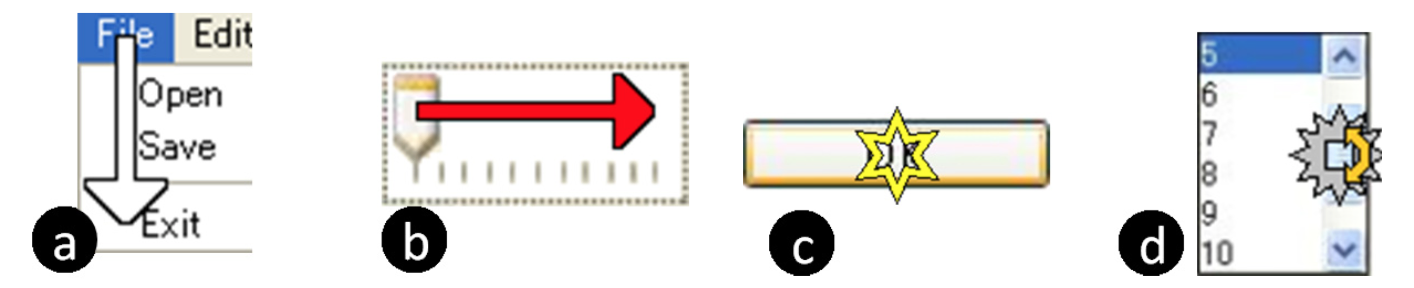
\includegraphics[width=0.6\textwidth]{\background/fig/software_viz/Nakamura_and_Igarashi}
  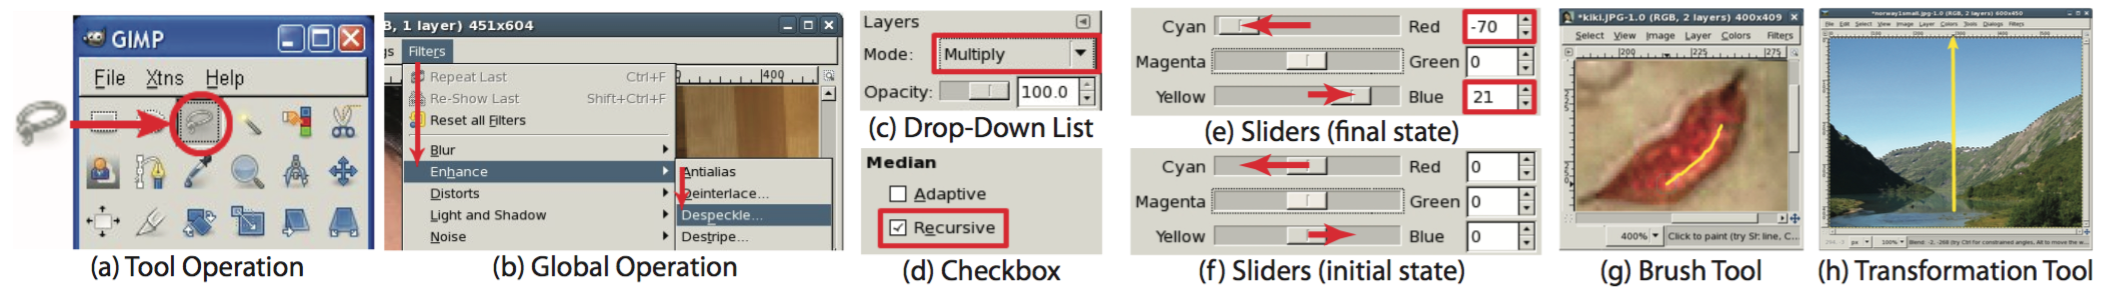
\includegraphics[width=\textwidth]{\background/fig/software_viz/Grabler}
  \caption{Example screenshots that visualize mouse operations are automatically rendered, including (top) mouse move, drag, click, and wheel (a-d) by Nakamura and Igarashi~\cite{Nakamura:2008:ASV:1449715.1449721} and (bottom) application-specific operations (a-b), parameters (c-f), and manipulations (g-h) by Grabler \ea{}~\cite{Grabler:2009jj}.}
  \label{fig:related_events}
\end{figure*}

To compare operation effects and workflows, other effective visualization approaches include showing a list of ``before'' and ``after'' thumbnails, video clips, and event timeline \cite{Grossman:2010jz} and creating a union graph of operations \cite{Kong:2012:DTR:2207676.2208549} (see Figure~\ref{fig:related_comparison}).

\begin{figure*}[t!]
  \centering
  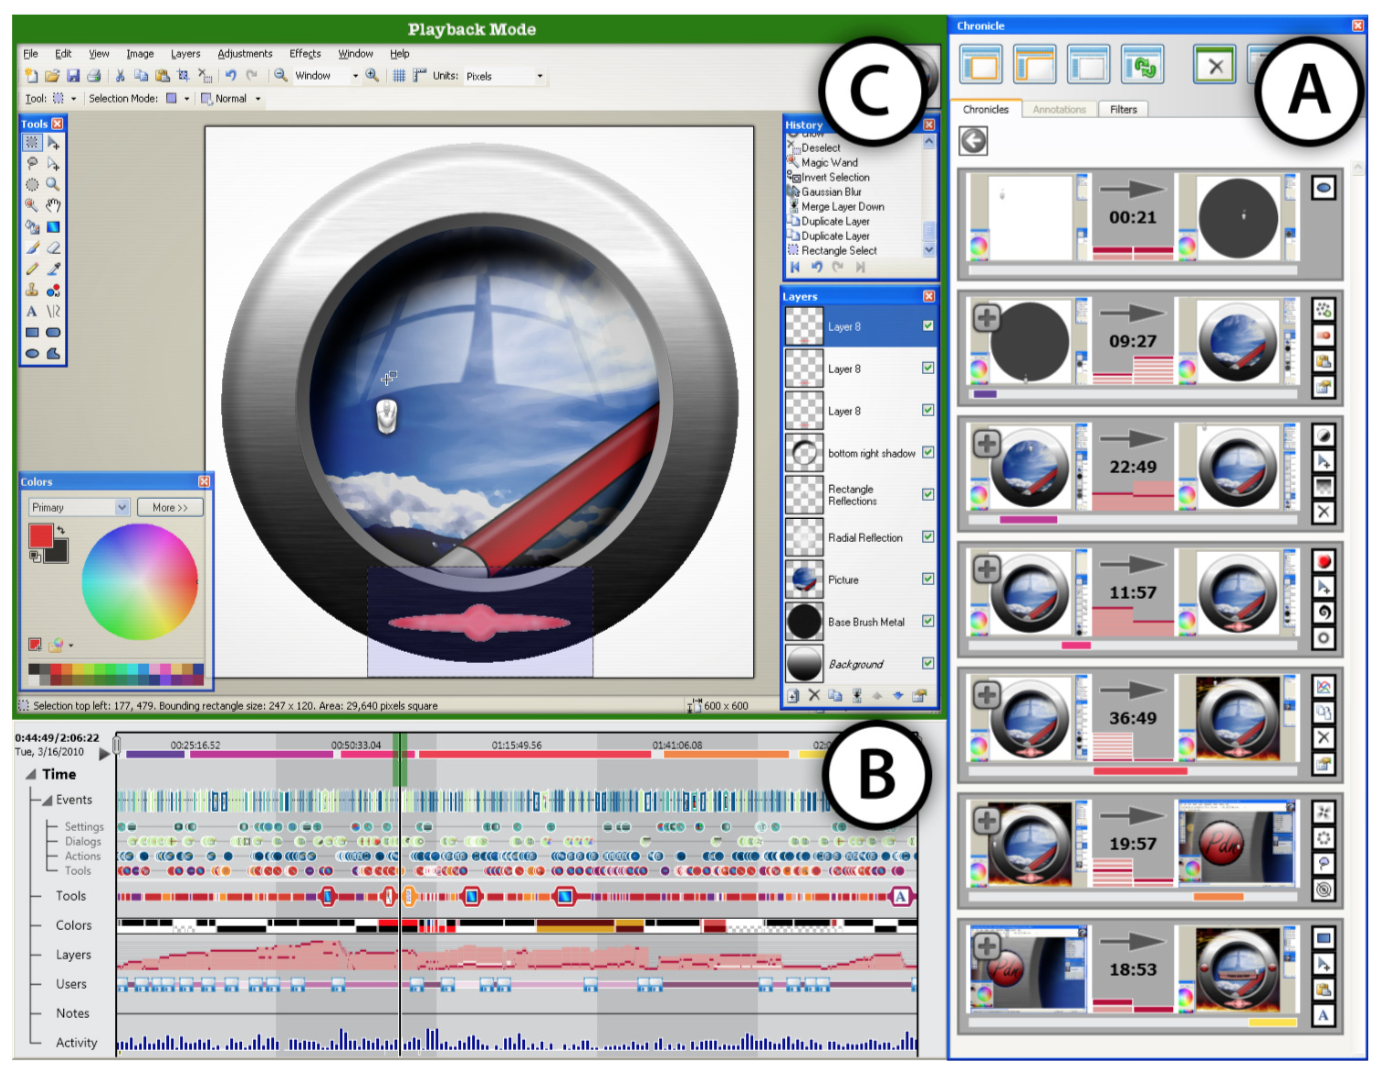
\includegraphics[width=0.4\textwidth]{\background/fig/software_viz/Grossman}
  \includegraphics[width=0.55\textwidth]{\background/fig/software_viz/Kong}
  \caption{Instructional systems that help learners compare effects and similar tutorials using: (left) before and after images (a) and event timeline (b) by Grossman \ea{}~\cite{Grossman:2010jz} and (right) operation union graph by Kong \ea{}~\cite{Kong:2012:DTR:2207676.2208549}.}
  \label{fig:related_comparison}
\end{figure*}

% -------------------

\subsection{In-Application Support}

The above systems introduce innovative ways of providing informative screenshots or representations for learners to review workflows. However, reviewing these materials is often separated from operating a software application. Learners might have to switch between context of interacting an application and reading instructions, which could introduce a gap of evaluation (\iquote{Am I doing this right as the instructions explain?}) and a gap of execution (\iquote{How do I perform the action that the instructions describe?}).
%
Researchers have proposed another approach to provide ``in-application'' assistance, often in real-time, in a specific application context.

Studies have shown that visualizing input events in real-time during operations can provide better learnability of applications \cite{Dixon:2010fb}.
%
Commercial tools such as Mouseposé\footnote{Mouseposé \url{http://www.boinx.com/mousepose}} and ScreenFlow\footnote{ScreenFlow \url{http://www.telestream.net/screenflow}} visualize mouse and keyboard events with special effects, such as drawing a circle around a mouse cursor (see Figure~\ref{fig:related_realtime} top).
%
Dixon \ea{} proposed techniques to provide pixel-based enhancements in real-time, such as highlighting nearest regions of interest or applying afterglows based on the current user operations \cite{Dixon:2010fb,Dixon:2011:CHP:1978942.1979086} (see Figure~\ref{fig:related_realtime} bottom).

\begin{figure*}[t!]
  \centering
  \includegraphics[width=0.7\textwidth]{\background/fig/realtime/realtime}
  \caption{Real-time visual enhancements on GUI applications: (top) Mouseposé highlights mouse cursors or text input; (bottom) Prefab creates target-aware or afterglow effects during user operating~\cite{Dixon:2010fb}.}
  \label{fig:related_realtime}
\end{figure*}

Real-time visual effects help users focus on the region of interest in a GUI application, but to support learners comprehend the application functionalities, there has been a considerable amount of research devoted to offering interactive helps.
%
Video snippets can be embedded in application tooltips~\cite{Grossman:2010wr}, which were shown to be seven times more effective than conventional tooltips for completing unfamiliar tasks.
%
Interactive, step-by-step instructions can be integrated in several forms:
%
To help user identify the correct UI components, tutorials can be shown via translucent colored ``stencils,'' which visually direct user's attention directly in an application~\cite{Kelleher:2005:STD:1054972.1055047}.
%
By tracking user's current operations, tutorials can be embedded in an application to provide instant feedback such as a check-mark or a percentage match~\cite{Fernquist:2011:SRE:2047196.2047245}, automatically replayed to provide the corresponding video instructions~\cite{Pongnumkul:2011ju}, or be shown as ambient help~\cite{Matejka:2011:AH:1978942.1979349}.
%
Instructions can be captured from demonstration as ``scripts'' for step-by-step navigation~\cite{Bergman:2005:DocWizards}. Having more user controls~\cite{Lieberman:2014:SML:2557500.2557543} or being enhanced with game elements~\cite{Li:2014:CGM:2556288.2556954, Dontcheva:2014:CCL:2556288.2557217} can further engage users in learning.

Last but not least, as tutorials are built for a broader community with a set of authors and learners, content can be dynamically updated within a community based on user contribution~\cite{Lafreniere:2013ff,Matejka:2009:CCR:1622176.1622214, Bunt:2014:TPI:2556288.2557118}.

interactive-visualization~\cite{Kwon:2016:CEO:2858036.2858101}
the paper that cited DemoWiz~\cite{Nguyen:2015:MST:2702123.2702209}

% These projects show how effective instructional representations can assist learners in learning or executing tasks. Our goal is to further study new formats that incorporate advantages of several formats of multimedia, including images, text, and videos, and in turn enhancing the learning experience for a variety of tasks.

% * define ``automatic''
% Note: MixT tutorials are automatically rendered from manual demonstration, not automatically generated.

% To provide real-time assistance, it is important to recognize the user activities during a task performance. Several domains have been widely studied, including software operations, scene recognition, and object tracking in a physical world.

% -------------------------------------------

\section{Instructions for Physical Activities}
\label{related_physical}

The above approach of tracking user behavior to automate tutorial authoring opens the door to interactive tutorials that can respond to user progress. However, tracking user behavior in the physical world, rather than in software, remains a challenge.

\subsection{Generating Instructions for Real-World Tasks}
Researchers have investigated tools for automatically generating visual instructions for physical tasks~\cite{feiner:1985:AEA:1299975.1300548,Seligmann:1991:AGI:127719.122732}. Workflows can be captured and created for furniture \cite{agrawala2003designing} or block assembly tasks \cite{Gupta:2012ku}.
%
If video content is difficult to be extracted, crowdsourcing algorithms have been introduced to structure step-by-step videos by online workers~\cite{Kim:2014:CSI:2611222.2556986}.
%
% New devices to support authors capturing multi-media materials, such as a turntable~\cite{Tseng:2015:SPT:2771839.2771869}
% documentation \cite{Tseng:2016:makeology}

\subsection{Interactive Guidance}
To provide responsive instructions, a computer system needs to understand user operations in real-time. Ideally, activities should be automatically tracked without human labeling.
%
Computer vision techniques can track specific physical targets, including hands \cite{Ranjan:2008}, user movements \cite{Wilson:2012fb}, fast-moving objects (e.g., a Ping-Pong ball) \cite{Okumura:2011tr}, or regions in pre-defined spaces \cite{Ranjan:2007}.
%
These methods usually require an expert defining heuristics of space regions or movement classifications ahead of time for the tracking program.
%
Thanks to the advance of technology, camera sensors such as Kinect have become widely available to track activities for block assembly~\cite{Gupta:2012ku} and dance~\cite{Anderson:2013:YEM:2501988.2502045}.

Real-time guidance is often shown via an external display, placed next to the working area~\cite{Gupta:2012ku}. To better blend the information into activities, Knibbe~\ea{} design a display-embedded table as a physical workspace that monitors, records, and assists users~\cite{Knibbe:2015:SMI:2817721.2817741}.
%
Alternatively, information can be overlaid on top of the work area using augmented reality, usually through a head-mounted display. Such systems can provide visual highlights for machine maintenance~\cite{Henderson:2011ff}, or interactive remote tutoring for repair tasks~\cite{Gurevich:2012ko}.
%
Another method is to overlay guidance on an augmented mirror for tasks such as dance movements~\cite{Anderson:2013:YEM:2501988.2502045}.

for Frisbee players~\cite{Solomon:2014:UTI:2540930.2540965}

% Lovell and Buechley use electrical sensing with conductive thread for a sewing tutorial~\cite{Lovell:2010tl}.

% I aim to propose a new approach that gives users flexibility in a home environment, and provides interactive control. If activity recognition is not possible, my approach includes users in the loop to annotate high-level information in order to create high-quality results.

% -------------------------------------------

\section{Working with Videos}

\tofix{intro here}

\subsection{Capture}
Several research and commercial systems guide users at capture time to yield higher-quality videos. Such systems often employ templates to help users capture sequences of distinct shots (e.g., Snapguide\footnote{\url{http://snapguide.com/}}) or suggest framing of the subject or camera view as in NudgeCam~\cite{Carter:2010}. Computer vision algorithms, like face tracking, can be used to offer real-time feedback during such directed actions~\cite{Davis:2003cu,Heer:2004ba,Carter:2010}. Instead of relying on templates, shot suggestions can also be bootstrapped through user dialogs~\cite{Adams:2005}.

\subsection{Annotation}
Researchers have investigated how to provide interactions that enable efficient, fluid annotation of video data, from the early EVA system~\cite{Mackay:1989} to more recent interfaces like VideoTater that leverage pen input~\cite{Diakopoulos:2006vt}.

\subsection{Editing}
Frame-based editing of video is very time-intensive, as it forces users to operate at a very low level of detail. Editors can leverage metadata, such as transcripts~\cite{Berthouzoz:2012,Pavel:2014:VDB:2642918.2647400} and shot boundaries~\cite{Casares:2002dx}, to give users higher-level editing operations at the shot level rather than the frame level.
In specific video domains like interview videos, transcripts can help users place cuts and transitions~\cite{Berthouzoz:2012}.
%
Computer vision techniques can automate certain effects, such as creating cinemagraphs~\cite{Bai:2012, Joshi:2012}, automatically-edited lecture videos~\cite{Heck:2007}, zoomable tapestries~\cite{Barnes:2010} and synopses~\cite{Pritch:2009vl}, or stabilizing shaky amateur videos~\cite{Liu:2011}. When analyzing video is a matter of subjective taste, identifying salient frames can also be outsourced to crowd workers~\cite{Bernstein:2011uj}.

live authoring through compositing and editing of streaming video~\cite{Freeman:2014:LLA:2611105.2557304}

\subsection{Navigating}
Videos can be navigated at the content level beyond log events, such as visualizing subject movements in a storyboard design \cite{goldman2006schematic} and enabling direct manipulation of a target in 2D \cite{Dragicevic:2008:VBD:1357054.1357096,Goldman:2008:VOA:1449715.1449719,Karrer:2008:DDM:1357054.1357097} or 3D \cite{Nguyen:2013:DMV:2470654.2466150}. These techniques help viewers understand content flow and playback videos, and have been applied to screencast videos \cite{Denoue:2013:RDM:2451176.2451190}. It is also possible to automate video control based on user actions for scenarios such as operating software applications~\cite{Pongnumkul:2011ju} and block assembling tasks \cite{Gupta:2012ku}. Such novel forms of video navigation inspired us to explore new visual designs for revealing the video content that support live presentations.

lecture videos~\cite{Tang:2006:DIU:1111449.1111523}

Visualization of personal history for video navigation~\cite{Al-Hajri:2014:VPH:2611105.2557106}

% In contrast to these systems, we do not require the author to manipulate the camera or system during capture. Many leisure activities, such as home repair or cooking, require use of both hands or involve getting one's hands dirty, so camera manipulation is not possible. We use vision techniques for automatic recording and editing. It differs from previous approaches in its focus on particular application domains -- software and physical demonstrations. By focusing on specific domains, we can make assumptions about the structure of the input and output video, such as the fact that there is a linear set of steps or movements, and offer user interfaces and algorithms that make it easier to create high quality instructions.

%!TEX root = ../thesis.tex
\section{Design Guidelines}

To motivate and inform the design of a tool to support live presentations, we collected preferences for software demonstrations using an online survey. We describe the three design goals derived from the survey results.

\subsection{Understanding Demo Preferences} To understand both presenters' and audiences' preferences for performing and viewing system demonstrations, we conducted an online survey in a software company and a university research lab. Our goal was to collect people's feedback on giving and seeing software demonstrations during live presentations. We received 73 responses from researchers, graduate students, software engineers, and designers. Their main research areas include human-computer interaction (64.4\%), software engineering (21.9\%), and machine learning (20.6\%); 66.7\% were male. Among all the respondents, 35.6\% indicated that they were very experienced at giving software demos to the audience during a live presentation; 46.6\% had demoed at least once; 13.7\% had not demoed but attended talks that showed a software demonstration.

We asked respondents who had demo experience (\textit{N} = 60) how they preferred to perform a demo. Their answers were: a live demo (25 out of 60), pre-recorded videos (15), a mixed format of a live demo and videos (12), static screenshots (4), and other (4). In Table~\ref{tab:demowiz_survey}, we list the top 2-3 reasons for their preferences. Giving a \textit{live demo} can be more engaging with a working system and match the audience's interests, but presenters can encounter unexpected problems and forget to show important features within a given time constraint. On the other hand, presenting with \textit{a demo video} avoids such problems by extracting the most important parts, and can allow visual highlighting (labeling or zooming), but can be less engaging. In addition, it is hard to narrate.

We were also interested in reactions as an audience member. For respondents who had seen software demos (\textit{N} = 70), we asked how they preferred to see the demonstration performed. We found a slightly different preference: a live demo (36 out of 70), a mixed format of a live demo and videos (24), pre-recorded videos (7), and other (3). However, the reasons were well aligned with presenters’ concerns. A\textit{ live demo} shows a working system and can be more engaging, but the audience might need to wait for system problems to be resolved or sometimes see presenters rambling. A\textit{ demo video }can show the most important parts, sometimes assisted by visual highlighting, but it can be hard to tell which parts of a demo are real, and can be less engaging to the audience.

\subsection{Design Goals} From the survey results, we understand that giving a live demo is often more preferable than showing demo videos. However, we cannot, in general, address some of the main concerns with giving a live demo – that is, stability of the software system and variations in the presentation environment which can cause the demo to fail. Therefore, we instead aim to address some of the drawbacks with demo videos while preserving their advantages. More specifically, our goal is to make demo videos \textit{more engaging} by assisting presenters in adjusting their narration to guide the audience through the material. In this section, we describe our design goals to support more effective demo video presentations.

\subsubsection{G1. Show what's coming next, where and when it will occur.}
To engage the audience with the demonstration, it is important for presenters to guide the audience's attention to the right place at the right time. To do so, presenters should be fully aware of upcoming actions – specifically \textit{what} actions will happen, \textit{where} they will occur on the screen, and \textit{when} they will happen.

\subsubsection{G2. Minimize required attention or interpretation.}
While it is our desire to help presenters understand and anticipate impending events, we should not overburden a presenter who is already narrating a specific set of talking points. As a tradeoff between providing more information and minimizing cognitive load, any augmentation of the video needs to be offered in a glanceable fashion, i.e., information can be interpreted quickly and without the presenter's full attention.

\subsubsection{G3. Support light-weight editing during rehearsal.}
Different presentations may require more or less extensive explanations, and when first recording a demo video, it may not be possible to perform the demo at the same rate necessary for a live presentation (e.g., typing can be difficult or system response times may be variable). In addition, it should be easy to review, practice, and modify the pace for a particular presentation. For all these reasons, lightweight editing and rehearsal are necessary.  Using these principles as a guiding rubric for our design, we iterated on several versions of the DemoWiz system.

\begin{table}
  \centering
  \includegraphics[width=\columnwidth]{\demowiz/fig/survey}
  \caption{Survey of software demonstration preferences from presenters' (N=60) and audience's (N=70) point of views.}
  \label{tab:demowiz_survey}
\end{table}

%!TEX root = ../thesis.tex
\section{Computer-Generated Visualization}

\subsection{Augmented Workflow}
For presenters to narrate ``live'' over a video recording, we propose augmenting a typical workflow from capturing a screencast video; to rehearsing it and adjusting timings; and finally to live presentation of the demo video (Figure~\ref{fig:demowiz_workflow}).

DemoWiz first captures a screencast video and input events during a software demonstration from a user-defined rectangular region. Once the recording is done, DemoWiz analyzes the low-level event stream and transforms it into higher-level events such as mouse clicks, double-clicks, and drags. DemoWiz then allows presenters to edit the timing and notes while practicing their presentations with the presenter view equipped with an adjustable event timeline (Figure~\ref{fig:demowiz_teaser}A). Finally, presenters can give a live presentation using the same UI (i.e., presenter view) and show the audience view without visualization to the viewers.

\begin{figure*}[t]
  \centering
  \includegraphics[width=0.7\textwidth]{\demowiz/fig/demowiz_workflow}
  \caption{DemoWiz workflow: Presenters captures a software demonstration, edit the video recording while rehearsing with our playback UI, and present the edited video to the audience using a presenter view.}
  \label{fig:demowiz_workflow}
\end{figure*}

% ---------------------------------------------------------------

\subsection{Visualizations}
To enable presenters to focus on their narration and the original video contents, DemoWiz augments the screencast recording by automatically overlaying simple glyphs.

\subsubsection{Input Event Glyphs}
DemoWiz overlays visual annotations of events on the screencast recording in a graphical way where the events happen.For example, in Figure~\ref{fig:demowiz_teaser}, the presenter clicks and drags the map view to the right. DemoWiz uses the following simple,distinctive glyphs to differentiate event types as Figure~\ref{fig:demowiz_glyphs} shows:

\begin{itemize}
  \item Mouse click: a red circle with a radius of 20-pixels,
  \item Double-click: a green circle with a radius of 20-pixels,
  \item Mouse drag: a thin, orange line with a dot at the start point and an arrowhead at the end point,
  \item Mouse scroll: a thin, yellow line, 80 pixels long, with an arrowhead, and
  \item Keystrokes: text in blue.
\end{itemize}

At any given time during the video playback, DemoWiz shows the current event and the upcoming event on the video. We tried to show more than two events within a fixed time period in our initial prototypes. However, we noticed several issues. First, the view becomes too cluttered to understand at a glance, especially when the original video is visually complex. Second, it is not easy to convey the order of the events. Third, it is difficult to observe when multiple events are spatially close. Therefore, we provide minimum but essential events for recall.

\begin{figure*}[t]
  \centering
  \includegraphics[width=0.7\textwidth]{\demowiz/fig/event_types/types}
  \caption{DemoWiz visualizes input events in a graphical way. From the left to right we show a mouse click, double-click, a drag, a mouse scroll, and keystroke events. These glyphs are overlaid on the video recordings.}
  \label{fig:demowiz_glyphs}
\end{figure*}

% --------------------------------------------------

\subsubsection{Visual Guides to the Next Events}
In order to help guide the presenter's attention, DemoWiz overlays a motion arrow between the current and upcoming events on the demo video (Figure~\ref{fig:demowiz_teaser}C). This is inspired by storyboard design used in filming where an arrow effectively shows the movement of a camera or an actor in a single shot \cite{goldman2006schematic}. We expand the idea of guiding attention for a specific purpose: the arrow in DemoWiz shows the movement from one action (e.g., click a checkbox) to another action(e.g., click a button). By overlaying this motion arrow, the visualization matches the flow of a presenter's attention when they observe the video content.

Since the distance between two consecutive event segments vary, we created three visual designs to make sure the arrows are visible to lead a presenter's attention:

\begin{itemize}
  \item For two events that are located far away (e.g., clicking an ``OK'' button after selecting a checkbox on a page), apply a \textit{straight} arrow (see Figure~\ref{fig:demowiz_arrows}A).
  \item For events that are nearly at the same location (e.g., click the ``Next'' button twice to navigate a list of selections),apply a \textit{round} arrow that points to the current location (see Figure~\ref{fig:demowiz_arrows}B).
  \item Otherwise, apply a \textit{curved} arrow (see Figure~\ref{fig:demowiz_arrows}C).
\end{itemize}

\begin{figure*}[t]
  \centering
  \includegraphics[width=0.6\textwidth]{\demowiz/fig/arrows/arrows}
  \caption{Three types of motion arrows in DemoWiz that guide presenters to the next event of different distances at a (A) far, (B) nearly the same, and (C) near location.}
  \label{fig:demowiz_arrows}
\end{figure*}

% --------------------------------------------------

\subsubsection{Sense of Timing}
DemoWiz provides a sense of timing for an upcoming action so that presenters can adjust their narration. First, DemoWizembeds \textit{a progress bar} in the motion arrow to show relative time (Figure~\ref{fig:demowiz_teaser}C). The green bar shows the proportional time that has been passed before reaching the next event (Figure~\ref{fig:demowiz_timing} top). When a motion arrow is filled up with green, it fades away and guides the presenter to the next action. We were concerned that people may associate the length of an arrow to the length of time. Therefore, we also incorporated a \textit{countdown} visualization where circles will fade out in the last three seconds before the next action starts (Figure~\ref{fig:demowiz_timing} bottom) to convey absolute timing.

\begin{figure*}[t]
  \centering
  \includegraphics[width=0.6\textwidth]{\demowiz/fig/progressbar/progressbar}
  \includegraphics[width=0.6\textwidth]{\demowiz/fig/countdown/countdown}
  \caption{A progress in time guides the presenter from the current event (left) gradually to the upcoming action (right) using relative timing with a progress bar (top) and absolute timing (bottom).}
  \label{fig:demowiz_timing}
\end{figure*}

% --------------------------------------------------

\subsubsection{Visualization Examples}
Figure~\ref{fig:demowiz_examples} presents examples of DemoWiz visualizations with four different systems. The glyphs effectively show the start and end points of mouse drags and the locations of mouse clicks. Motion arrows help direct the presenter's attention between events, such as start the end of the drag event to clicking a button (Figure~\ref{fig:demowiz_examples}A and B), clicking between several options (Figure~\ref{fig:demowiz_examples}C), or selecting a specific slide after scrolling down (Figure~\ref{fig:demowiz_examples}D).

\begin{figure*}[t]
  \centering
  \includegraphics[width=0.7\textwidth]{\demowiz/fig/examples/examples}
  \caption{Examples of DemoWiz visualizations with four different systems and input event sequences.}
  \label{fig:demowiz_examples}
\end{figure*}

% ---------------------------------------------------------------

\subsection{Lightweight Editing During Rehearsal}
During rehearsal for their demonstration, presenters can modify the video timing and add reminder notes for their narration. DemoWiz shows the type and length of each event in a sequence in a timeline (Figure~\ref{fig:demowiz_teaser}A). Each segment is shown as a block whose width indicates its length in time. To simplify the timeline and avoid fine-grained adjustment,lengths of event blocks are rounded to the second. Presenters can modify the playback speed of a segment by dragging the boundaries of a segment on the timeline. For example, presenters can speed up to shorten long text inputs, and slowdown for fast mouse drag inputs that select multiple objects.

Sometimes a change in the playback speed may result in an awkward effect that is noticeable to the audience, especially when showing a UI transition. Therefore, DemoWiz supports two special time control markers to enable breaks in the narration. Presenters can add an adjustable \textit{pause} segment, at which the system will pause at the last frame of the previous segment for the specified length of time. If presenters prefer full control on pause length, a \textit{stop} marker ensures the video stays paused at the last frame of the previous segment and will not proceed until presenters manually resume the playback of the video.DemoWiz enables presenters to add a short text note (such as the reminder \iquote{Move and zoom...} in Figure~\ref{fig:demowiz_teaser}) so that they could remind themselves of upcoming actions at a higher level. The note can be positioned manually at any location on a video so that it does not block important video content, and will be shown for 3 seconds before the associated event.For every edit that is associated with time changes (including playback speed and pauses), DemoWiz computes and updates the total presentation time as well as updating the progress bar and countdown to provide accurate timing.

% ---------------------------------------------------------------

\subsection{Presenter View}
During presentation, DemoWiz shows two views in separate windows. Presenters can observe visualizations using the presenter view, while the audience will see the audience view with a full-screen video that has no enhanced information. DemoWiz synchronizes the videos in both views based on presenters' editing decisions to ensure the same playback speed and time. As with a conventional video player, presenters can control the video, to pause and play at any time. In addition, when a video is paused (or stopped), presenters can hover the mouse over the demo video in the presenter view to point out an important area, as many presenters currently do in a live demo. DemoWiz then simulates and synchronizes a mouse cursor in the audience view to help the audience follow the demonstration.

% ---------------------------------------------------------------

\subsection{Implementation Details}
During recording, DemoWiz captures the screen within a specified region and logs low-level system input data with\textit{timestamps} (with an accuracy of 0.1 seconds) from the operating system, including:

\begin{itemize}
  \item \textit{Mouse events} (mouse downs, mouse ups, and mouse wheel movements) and their \textit{positions} (in x-y coordinates relative to the screen-captured region).
  \item \textit{Key-press events} (keyboard input).
\end{itemize}

Once presenters finish their demonstrations, DemoWiz analyzes the low-level event stream and transforms it into high-level event metadata. For mouse events, we pair each mouse down and up into mouse \textit{clicks}, \textit{double-clicks}, or \textit{drags}. We group any consecutive mouse wheel events within a time threshold of 2 seconds to one \textit{scroll} event and any key-press events within the same threshold to one \textit{keystroke} event(e.g., combine keys d-o-w-n-t-o-w-n to ``downtown''). For each high-level event, we log the \textit{start} and \textit{end time} (timestamps of the first and the last low-level event).

Based on the start and end times of these high-level events, DemoWiz segments the screencast video recording into \textit{event segments}. Any gap between two consecutive input events is marked as an \textit{inactive segment}, which may include mouse hovering, UI transitions of the demo system, or static frames with no visual changes. DemoWiz adjusts the boundaries of these event segments to avoid any short visual effect that cannot be observed. DemoWiz examines segments in a linear order to ensure each segment lasts at least $t_{min}$ seconds long,which is set as one second based on our early testing. For an event segment $S_i$ of time ($t_{start}$, $t_{end}$) that $t_{end} - t_{start} < t_{min}$, DemoWiz expands 0.5 second forward and backward if $S_{i-1}$ and $S_{i+1}$ are inactive. If the adjusted $S_{i-1}'$ and $S_{i+1}'$ are shorter than $t_{min}$, DemoWiz merges it to the shorter neighbor segment. Currently, DemoWiz does not analyze these inactive segments, but techniques including computer vision and video analysis \cite{Banovic:2012kd,Chi:2012:MAG:2380116.2380130} can be applied for finer segmentation.

The capturing program is implemented in C\#. Two APIs were used: 1) the Windows Event Log API for mouse and keyboard hooks and 2) the Expression Encoder 4 API for screen recording running on Microsoft Windows 7. The recorded metadata(stored in a JSON object) and screencast video (in MP4) are read by the Presenter UI, which is implemented using standard Web technologies, including HTML5, CSS3, JavaScript, and jQuery. In particular, the visualization is rendered on the canvas element on top of the video object on the fly based on the video playback time. The audience view is generated by the main browser window of presenter view for video control.

%!TEX root = ../thesis.tex
\section{Evaluation}
To evaluate the DemoWiz design, we conducted a controlled experiment in which participants recorded and edited a demo video, and gave a presentation with the edited video. Specifically, we wanted to see if presenters would evaluate their own performances higher with the support of our augmented visualizations and control of timing.

\subsection{User Study}

\subsubsection{Baseline Condition: DemoWiz without Visualization}
Since DemoWiz allows for rapid editing of the video, it would have been unfair to compare it with a conventional video player without supporting any editing during the rehearsal phase. We therefore modified our system to serve as the baseline condition, providing participants with the same lightweight editing of the video in each condition. However, during presentation, the baseline condition was similar to a conventional video player that shows only the video without event timeline and augmented visualizations. It also did not support the \textit{stop} markers and \textit{text notes}, i.e., participants could only adjust playback speed of each segment and add variable length \textit{pauses}. During presentation, participants only saw the video with a traditional timeline. They could, however, pause (or stop) and resume the video manually at any time during playback.

\subsubsection{Study Design}
We conducted the study as a within-subjects design in a usability room. After recording and editing a video using the same system, each presenter gave a presentation with both systems to an experimenter. To control the effect of order and learning, we prepared two tasks that included similar interaction flows and counterbalanced the order of the two systems—DemoWiz and Baseline—-but we fixed the order of tasks. Even though presenting to a single audience member in a usability room is not the same as using the system with a large conference audience, it is important to control the tasks and presentation as closely as possible to understand the relative benefits of the system in comparison with a baseline condition.

For each condition, we observed and coded the \textit{timing} of narration that matched the video content and noted the time in seconds when an event was described \textit{before}, \textit{at}, or \textit{after} the action happened in the demo video. We also marked obvious \textit{breaks} between narrations, \textit{errors} when the narration was not about the current or following events (e.g., discussing actions in a different order than they actually occurred), and \textit{misses} when an important action was not mentioned. To avoid unconscious bias that might influence the coding of the videos, we neutrally named the recordings and coded them all in a batch. We focused on objective timing measurements as much as possible, measuring deviation from specific video events and their corresponding narrations down to a second. Finally, we gathered qualitative feedback through satisfaction and preference questionnaires.

\subsubsection{Participants}
We recruited 12 participants (10 males and 2 females) from a software company. However, we excluded the data from two participants (1 male and 1 female); one was due to a software bug during one condition and another was because the participant requested to restart a presentation in one condition. The average age of the effective 10 participants was 37.3 ranging from 24 to 64 years of age. We recruited participants who had experience at showing a software demonstration to an audience such as giving a presentation at a conference. Four participants were native English speakers and the rest were fluent in English. The expertise of participants included audio processing, computer graphics, human-computer interactions, machine learning, networking, and software engineering. Each participant was compensated with lunch coupons worth \$20.

\subsubsection{Procedure and Tasks} Each session consisted of one training task and two experimental tasks. For the training task, to introduce the common features for recording and editing the video, we designed a simple workflow of five steps to demonstrate editing of a slide using PowerPoint. The experimenter briefly demonstrated an example and then introduced the recording program that captured the screen. Participants were then asked to practice and record using the recording program.

The two tasks consisted of a similar sequence and interactions: 1) searching with Bing Maps to show the 2D map view and the Bird's Eye view, looking for a restaurant, and navigating to the interior view of a specific restaurant; and 2) searching with Google Shopping to show the search results with the Grid view, filtering and voting for reviews, and navigating the 3D product view of an espresso machine. For each task, we provided a specific scenario along with a list of subtasks. The experimenter walked through this list with participants to ensure that they could easily find the features that needed to be demonstrated. Participants were then asked to practice (3-5 minutes), record (about 2 minutes), and rehearse and edit (5-10 minutes).

To help simulate a conference setting where participants would not be able to present immediately after having recorded a demonstration, we inserted an intentional 1-minute gap between rehearsal and presentation. During this gap before giving the presentation, we asked participants to watch a conference showcase video. Participants were then asked to stand up and gave a 2-3 minute presentation to the experimenter in a usability room.

After each task, participants filled out a questionnaire of 8-10 questions asking about their experience (8 for the Baseline condition, and 10 for the DemoWiz condition). At the end of the session, an online questionnaire was provided for them to present overall preferences and leave comments. Each session lasted about 1.5 hours.

\subsubsection{Experiment Setup}
Each participant used a desktop computer running Windows 7, Expression Encoder 4 for screen recording, and a web browser for the DemoWiz user interface. A regular mouse and keyboard were provided, along with two 27-inch displays, one for editing (during rehearsal) and showing the audience view (during presentation), and the other for the presenter view on a stand-up table. The resolution of both displays was 1920×1200 pixels. The average captured screen area was 1311×857 pixels. In the presenter view, the video resolution was within 1000×600 pixels; in the audience view, the screencast videos were resized to fill the entire display with at least 100-pixel wide border in black. During the study, the experimenter stayed in the room, providing instructions and sitting behind the participants during the recording and editing phases.

% ---------------------------------------------------------------

\subsection{Results}
Ten participants successfully recorded, rehearsed, and gave a demo with both systems.

\subsubsection{Subjective Preference}
Figure~\ref{fig:demowiz_likert} shows the average subject responses (on the 7-point Likert scale) from presenters for both systems. We analyzed these subjective responses using a Wilcoxon signed-rank test. We found significant differences in responses for ease of narration (DemoWiz µ = 6.2 over Baseline µ = 4.5, \textit{p} = .018) and ease of presentation (6.4 over 5.2, \textit{p} = .048). We also found marginally significant differences in participants' overall satisfaction with their presentations (5.5 over 4.7, \textit{p} = .062). Participants also tend to agree that DemoWiz helped them interpret timing (6.1 over 4.4, \textit{p} = .067).

In addition, 9 out of the 10 participants preferred DemoWiz to the system without visualization and would choose to present with DemoWiz if they were asked to give a public software demo; the remaining participant indicated no preference for both questions. The general feedback was also encouraging. For example, P1 commented \iquote{Awesome system. I'd use it today.} and P5 \iquote{felt more confident in being able to present what I wanted to.}

\begin{figure*}[t]
  \centering
  \includegraphics[width=\textwidth]{\demowiz/fig/results/likert}
  \caption{User feedback from questionnaire on the 7-point Likert scale.}
  \label{fig:demowiz_likert}
\end{figure*}

\subsubsection{Visualization as a Supportive Cue}
Participants answered that they were able to understand DemoWiz visualization of input events (µ = 6.0) and found it supportive for their presentations (µ = 6.3). They also commented that the DemoWiz visualization supported the presentation in various aspects: \iquote{the visualization reminds of the order of the content} (P1), \iquote{Really liked the ability to know what was coming up} (P2), \iquote{It provides better insight of the progress of the video} (P6), and \iquote{viz gave me an idea about timing or something I was going to forget to say} (P9).

\subsubsection{Narration Timing}
We coded the 20 recordings of participants' final presentations to observe the timing of narration of each action in correspondence with the video content (11 key events for both tasks). With DemoWiz, participants tended to \textit{anticipate} the upcoming events rather than talk afterwards, where the average timing was -0.1 seconds with DemoWiz (i.e., narrated the action before it happened) and 0.4 seconds with the Baseline condition (i.e., explained the action after it was shown). We found a significant difference in the number of times that events were anticipated by the narration, co-occurred, or occurred after the fact ($\chi $\textsuperscript{2}\textit{(2,220) = 8.6, p = .01}, see Figure~\ref{fig:demowiz_results_timing}).

In general, this supports our suspicion that DemoWiz would help in anticipating an event as opposed to talking about it after it occurred. More important though, was how often a narrator spoke about an event within several seconds of when the event actually occurred. By defining \textit{better} timing as when a presenter's explanation came within 2 seconds of a shown event (either prior, exact, or after), there was marginal significance by condition (\textit{p} = .089 with DemoWiz performing better). In addition, with the Baseline condition, the timing of narration was less consistent and off more, varying from 6 seconds early or 10 seconds late with a variance of 3.9 seconds, in comparison to the DemoWiz condition with at most 3 seconds early to 3 seconds late and a variance of 1.9 seconds.

Five participants had an obvious \textit{error} (forgot the next action or incorrectly narrated another action), had a long \textit{break} (waiting for more than 2 seconds until the action was made), or \textit{missed} an action (did not explain an important feature) when presenting with the Baseline condition. On the other hand, in the DemoWiz condition no errors were made, and there were only one long break and one miss from two different participants, respectively.

Participants' comments also support the fact that DemoWiz helped presenters anticipate the upcoming events. P7 explained, \iquote{(I) felt better able to time my speech to coincide with visual events, rather than trailing after them. Without the event visualizations, I felt like I was talking about what the audience had just seen, rather than having my words and visuals combine to a single message.}

\begin{figure*}[t]
  \centering
  \includegraphics[width=\textwidth]{\demowiz/fig/results_timing}
  \caption{The number of times events were anticipated by the narration, co-occurred, or occurred after the fact.}
  \label{fig:demowiz_results_timing}
\end{figure*}

\subsubsection{Editing Experience}
We collected comments on the workflow. Participants found it easy to record (µ = 6.4) their demonstrations with DemoWiz. For editing features, they found it easy to edit in general (6.6), including controlling the playback speed (6.5) and adding pauses and stops (6.5), but it was less easy to add text notes (4.8); only two participants used this as reminders.

Although using different strategies, all of the participants adjusted the playback speed for matching their narration. Some sped up whenever possible and added stop markers for transitions; some slowed down the repetitive actions (such as drags) to demonstrate effects. P6 said, \iquote{I really liked being able to add ‘stop' events so I could \'fake\' my demo better.} DemoWiz made it easy for participants to separate the capturing and presentation preparation as P5 explained, \iquote{Overall, recording was very easy. In fact, as I got to the second task, I realized that I really don't need to think about the words as I record because later on I will be able to slow down and speed up time ...}

On average, the length of demo videos was 2'09\" before editing and 2'05\" after editing, and the presentation was 2'38\" long. Each participant spent 7.5 minutes on average to edit. For each demo of 44 segments on average, participants adjusted 3.15 segments for speedup and 4.25 segments for slowdown, and added 0.55 pause markers. In the DemoWiz condition, 1.2 stop markers and 0.2 text notes were added.

%!TEX root = ../thesis.tex

\subsection {Discussion}

%We discuss general findings from the 3 studies.
% \dan{Make this a discussion about all 3 studies together, what was learned overall? Argue that DemoDraw is good.}
%
Participants were clearly excited about the overall experience using both the \phaseI{} and the \phaseII{}.
%Comments we received included, \systemname{} is a \iquote{REALLY COOL SYSTEM} (Study 2-P7), \iquote{Seriously, the poses look really cool! I want the last one to be my profile picture} (Study 2-P3), and \iquote{Great idea overall, this will save lots of time for whoever is designing these artworks :)} (Study 3-P3).
%
Some explicitly pointed out their enjoyment when using our system:
% \iquote{Overall, it's a lot of fun, and I can see it being really helpful for anybody trying to explain motion} (P3),
\iquote{it accurately captures how much fun I had making it. :)} (Study 2-P9), and
\iquote{For professional artists, the system not only increases their productivity, but also brings joy and fun to this kind of tasks} (Study 2-P10).

Participant feedback suggests motion illustrations generated by \systemname{} are expressive enough to depict their demonstrations. Our multi-modal interface with our motion analysis and rendering algorithms enabled users to quickly create step-by-step diagrams. Recall that current methods using existing software tools to create similar diagrams take significant time and making visual or spatial changes is difficult.

\bjoern{I'm not really sold on the rest of this section - some of it feels too low level. Not sure what to do here.}

\dan{One of the main things to discuss (with some convincing arguments based on specific results from the three studies) is whether we achieved our primary goals and answered research questions:
1) the system makes good looking diagrams quickly; (reference back to how long current methods take)
2) the iterative/interactive demonstration style is key to this success. (reference back to how non-iterative current methods are) }

\dan{Another discussion topic is the implications of this system. If the iterative/interactive demonstration style worked here, would it be better in other demonstration systems too? What should interaction designers learn from this at a level above the specific motion illustration task?}

\subsubsection{Illustration Styles}
In Study 1, motion arrows successfully conveyed the majority of movements. For some movements when arrows failed to express the intent, other illustration effects might clarify the details to depict the start, intermediate, and end poses. For example, in the first motion set of Study 1, the circular hand movements and squatting action of Step 3 might not be easily interpreted (see Table~\ref{tab:study1_errors}), but for the same motion, participants preferred stroboscopic effect that clearly showed the arm movements and transition in height (see Figure~\ref{fig:study3_effects}).

Furthermore, as \systemname{} captures the continuous motion sequence in 3D from a demonstrator, our system also generates animations showing the dynamic movements.
%
In the warm-up task of Study 2 that captured the second motion set in Study 1, some participants explained that the playback animation of the recording clarified the motion where they incorrectly interpreted the start position.
%
We propose that as motion arrows can efficiently and effectively express most of the motions, a mixed-media version can be created that has been shown to be useful for clarifying step-by-step instructions \cite{Chi:2012:MAG:2380116.2380130}, where viewers can selectively review part of a static diagram with in-place animation playback. In addition, the 3D reconstruction also makes it possible to review motions from different angles.
%
All in all, our technology enables both instructors and viewers to interactively create and review motion illustrations in multiple ways.

%!TEX root = ../thesis.tex
\chapter{Discussion}
\label{chapter_conclusion}

\section{Restatement of Contributions}
In this dissertation,

% How to design tutorial systems appropriately for different situations
% * level of expertise of instructor, learner
% * what are you trying to make easier?

\section{Remaining Challenges and Future Directions}

formal language
- now template, a set of techniques

\subsection{Collaborative Authoring}
a team, beyond a single author for larger projects or tasks

\subsection{Non-Linear Tutorials}
branching

\subsection{Mobile Capturing devices}
Tango, Structure Sensor, Leap Motion

\subsection{Emerging Instructional Space}

Augmented and virtual reality systems are becoming available to end users via affordable forms. However, designing AR and VR experiences extremely requires expertise and efforts. As devices offer personalized effects supported by sensing and input techniques, we need new authoring tools that focus on delivering story-centric experiences. Tools should also enable both professionals and amateurs to create and iterate designs efficiently in an immersive 3D world. ...research what future AR and VR creation tools would look like with new authoring processes.

by demonstration
``Microsoft HoloLens with Autodesk MotionBuilder'' by Jasper Brekelmans, \url{https://www.youtube.com/watch?v=yfl7pwXftUs}, licensed under CC BY 2.0


\begin{figure*}[ht!]
  \centering
\begin{tabular}{cc}
  \includegraphics[width=0.4\textwidth]{\conclusion/fig/ar/hololens_fix1} &
  \includegraphics[width=0.4\textwidth]{\conclusion/fig/ar/hololens_fix2} \\
\multicolumn{2}{c}{\includegraphics[width=0.82\textwidth]{\conclusion/fig/ar/hololens_skype} }
\end{tabular}
\caption{
  Microsoft's HoloLens~\cite{MicrosoftHoloLensSkype} has introduced an Augmented Reality application on providing real-time physical instructions from a remote instructor.
}
\end{figure*}

\section{Conclusion}
In this dissertation, we present video-based approaches designed for amateur users to produce and consume effective instructions from demonstrations. Using video and audio analysis techniques, our tools support recording, editing, and playback in a tutorial production process. We demonstrate results of our computer-generated tutorials from several domains, including software applications and physical activities. Our goal is to increase the quality of instructions created by tutorial authors and to support learners navigating and following the tutorials.


%!TEX root = ../thesis.tex
\chapter{DemoCut: Instructional Videos from Demonstration}
\label{chapter_democut}
% \chapter{DemoCut: Generating Concise Instructional Videos for Physical Demonstrations}

Amateur instructional videos often show a single uninterrupted take of a recorded demonstration without any edits. While easy to produce, such videos are often too long as they include unnecessary or repetitive actions as well as mistakes.

In this chapter, we introduce DemoCut\footnote{This work was published at UIST 2013~\cite{Chi:2013:DGC:2501988.2502052}.}, a semi-automatic video editing system that improves the quality of amateur instructional videos for physical
tasks. DemoCut asks users to mark key moments in a recorded demonstration using a set of marker types derived from our formative study.
%
Based on these markers, the system uses audio and video analysis to automatically
organize the video into meaningful segments and apply appropriate
video editing effects.
%
To understand the effectiveness of DemoCut, we report a technical evaluation of seven video tutorials created with DemoCut. In a separate user evaluation, all eight participants successfully created a complete tutorial with a variety of video editing effects using our system.

%!TEX root = ../thesis.tex
\chapter{Introduction}
\label{chapter_introduction}

When attempting to accomplish unfamiliar, complicated tasks, people often look for tutorials to follow instructions. From performing daily tasks such as cooking and operating a machine, using software applications, to physical activities like sports and dance performance, each domain involves specific ``how-to'' knowledge with a certain degree of complexity~\cite{ryle1945knowhow}.
%
Instructions, which describe how a specific goal can be accomplished, are a tool for people to self-learn a task~\cite{Smith03iimanufacturer}. Studies have shown that visual instructions are cognitively favorable by people as they are easier to comprehend and remember than text information~\cite{Harrison:1995uh,mayer1996less,Heiser:2004:IVC:989863.989917}. In history, pictorial instructions have been created from the Middle Age to explain dancing or weapon operations~\cite{mijksenaar1999open}. It was found that the first use of letters in technical drawing for text referral was by Italian polymath Leonardo da Vinci. In 1737, French engineer de B{\'e}lidor~\cite{de1737architecture}'s diagrams were the first to apply arrows to indicate direction of movements (see Figure~\ref{fig:intro_arrows}).
%
From 1760, when the Industrial Revolution introduced mass production, instructions have been seen widely for various products and uses.

\begin{figure*}[h!]
  \centering
  \begin{minipage}{\textwidth}
  \includegraphics[width=\textwidth]{\intro/fig/arrows/arrows}
  \caption[Uses of motions arrows in visual instructions.]{Uses of motions arrows in visual instructions:
  %
  a) Year 1737: The first use of a motion arrow in an illustration explains the impact of water flow of a water wheel~\cite{de1737architecture},
  % http://www.buw-output-archiv.uni-wuppertal.de/ausgabe1/steinle/index-en.html
  %
  b) Year 2002: Similarly, arrows are used to explain the water flow and rotation of an undershot water wheel\footnote[1]{Original artwork by Daniel M. Short, ``Schematic diagram of an undershot water wheel'', licensed under CC BY-SA 2.5},
  % https://en.wikipedia.org/wiki/File:Undershot_water_wheel_schematic.svg
  %
  c) Year 2014: An animation visualizes the blood flow using motion arrows\footnote[2]{Video by Bioscience Credentials, ``Blood Flow in the Human Body'', \url{https://youtu.be/GwX41xm9esY}, licensed under CC BY 3.0}.
  }
  \label{fig:intro_arrows}
  \end{minipage}
\end{figure*}

Since the late 1990s, the advance in computer technologies has introduced more versatile instructional design. Instructions can now be created via software tools rather than hand drawing; they can include multimedia such as images and videos in several forms; they can be accessed through the Internet, as well as in hard copy.
%  the general purpose computers and the Internet
%
This advancement also enables consumers or end-users to document and share their domain knowledge~\cite{Lafreniere:2012tl}. As of today, popular tutorial sharing sites like Instructables has over 220,000 articles~\cite{InstructablesProjects}, wikiHow provides over 192,000 articles~\cite{wikiHowStatistics}, Food.com serves over 500,000 user-generated recipes with 125,000 photos~\cite{FoodComAbout}, and YouTube hosts over 285 million How-To videos\footnote{YouTube, \url{https://www.youtube.com/}, accessed June 2016}.
%
The variety of topics, content, and presentation styles provides learners more options to understand domain knowledge.
%
However, navigating a tutorial using existing tools remains inefficient for following step-by-step instructions. It can be challenging to observe details from text and images or find specific piece of information in a video through a timeline with conventional video players.
%
On the other hand, producing high-quality instructions that are easy to follow requires authoring expertise and a significant time investment. It involves several stages to design, record, and edit multimedia materials of a task using a variety of creation tools~\cite{Torrey:2007he,Tseng:2014:PVP:2598510.2598540,Muller:2009tw}.\\

The goal of this dissertation is to investigate interactive instructional design and develop computational tools that support the authoring process.
%
To contribute to computational methods of authoring user-generated instructions, two research questions that this work focuses on are:

\begin{itemize}
  \item How can authoring tools support domain experts in efficiently creating effective, high-quality instructions based on video-recorded demonstrations?
  \item How can new tutorial formats help authors better express their intent and help learners understand and follow the author's instructions?
\end{itemize}

This dissertation presents video-based computational approaches that enhance tutorial creation and consumption from author demonstrations.
We encode the current practices from professional authors into automatic algorithms and interactive techniques.
Our goal is to dramatically increase the quality of amateur-produced video instructions, which in turn improves learning for viewers who interactively navigate the content.
%
We will introduce five interactive systems that we develop to address these challenges. These tools cover both software applications (e.g., image manipulation tasks or browser navigation) and physical activities (e.g., Do-It-Yourself projects or dance movements) for recording, editing, and replaying instructional content.

% ---------------------------------------------------------------

\section{Challenges of Creating and Consuming Instructions}

Visual instructions are the dominant form of instructional design~\cite{mijksenaar1999open}. Cognitive load theory of multimedia learning suggests that learners process information using distinct channels, one for visual and the other for verbal formats~\cite{sweller1998cognitive,sweller1988cognitive,paas2003cognitive}. It was found that learners performed better when received a pictorial summary of a scientific system than those who received the full text alone or the full text with the summary~\cite{mayer1996less}.

Among all the multimedia support, videos are a common form to present instructions. We suspect that the great popularity of videos is due to the following reasons:
%
First, consumer devices and software have become affordable for authors to quickly record activities and later share via online platforms at minimum cost.
%
% ** describe the difficulties of making knowledge "explicit", esp. for actions and motions
Second, videos can be an efficient medium to document activities. Transferring know-how concisely and effectively to the audience is challenging. It especially requires efforts when a task involves \emph{tacit knowledge}, which is a kind of knowledge that is difficult to articulate in a written or verbal form~\cite{polanyi1958personal, Klemmer:2006:BMF:1142405.1142429}. Examples of tacit knowledge include dancing, riding a bike, or driving nails with a hammer. Dancers can perform movements fluently with music. If they are asked to focus on the composite pieces, such as the arm and foot actions or rhythm, they might get confused and fail to express the entire movement~\cite{polanyi1958personal}. Very often, recording a video eases the difficulties of describing the entire activities in an explicit form.
%
This leads to another motivation that videos also provide an effective channel to convey ideas with adequate amounts of details. Learners can visually observe the exact actions in a video as if an expert were coaching in person~\cite{Kuznetsov:2010:REA:1868914.1868950}.

However, while videos are easy to produce, they can include a lot of unnecessary footage. Inevitable content such as pauses, mistakes, and long repetitive actions makes it difficult for learners to focus on the most important steps and actions. A lot of authoring effort commonly goes into extracting footage, applying visual effects, and adding subtitles and annotations.
%
In addition, even with a well-edited video, navigating using a conventional video player remains inefficient. Learners with various needs could have a hard time skimming to an interesting moment or perceiving high-level overviews. Alternatively, a pictorial summary or static step-by-step tutorials presented with text and images can effectively guide knowledgeable learners through familiar tasks.

% The goal of this dissertation to develop video-based recording, editing, and playback tools are optimized for creating and consuming instructional demonstrations. I combine the advantage of ubiquitous video recording with the benefits of video and structured tutorial formats. I aim to dramatically increase the quality of amateur-produced video instructions, which in turn improves learning for viewers who interactively navigate the content.

% ----- MixT ----- %

\subsection{New Tutorial Formats}

Both static and video tutorials have strengths, but neither format alone is well suited for all learning needs that learners may have.
%
To combine the benefits, we design a new instructional presentation called \emph{MixT} (mixed-media tutorials) that improves learners' success in following instructions (see Figure~\ref{fig:mixt_intro}).
%
MixT presents step-by-step static instructions and includes in-place video clips for each operation.
%
With MixT, learners can quickly scan forward and backward on a web page to obtain an overview of a task. Embedded videos help them understand continuous, complex manipulation, such as brushing on a canvas and adjusting control points.
%
MixT's playback UI allows learners to interactively control \emph{when} to see images or videos, and \emph{how} to render videos.
%
Video editing techniques are applied to emphasize instructions, including cropping salient screen regions and highlighting interaction.
%
In our within-subject experiment, MixT successfully reduced numbers of errors and attempts made by learners when following image manipulation tasks.
% To demonstrate , MixT captures screencast video and operation events of a software demonstration.

\begin{figure*}[t]
  \centering
  \includegraphics[width=0.8\textwidth]{\intro/fig/mixt_intro}
  \caption{MixT generates step-by-step tutorials (left) that contain static and video information from task demonstrations. Videos are automatically edited and offer different views (right) to highlight the most relevant screen areas for a step. Visualizing mouse movement helps learners understand a complex action.}
  \label{fig:mixt_intro}
\end{figure*}

% ----- DemoWiz ----- %
MixT offers a novel way of navigating instructional content with a combination of static step-by-step and embedded video presentations. If an author wants to narrate over a video recording to illustrate a demo, it can be challenging to pace oneself at the suitable timing without expecting \emph{when} and \emph{what} action is taking while a video is playing.
%
We design \emph{DemoWiz}, a system that augments a screencast video with visualizations (Figure~\ref{fig:demowiz_intro}). By logging the input events of a software demonstration, DemoWiz overlays glyphs to visually guide viewers to the next action along with the time remaining before the action occurs. This enables viewers to anticipate the video content rather than react to it.
%
Our study showed that fewer anticipation errors and narration delays were made with DemoWiz.

\begin{figure*}[t]
\centering
\includegraphics[width=0.7\columnwidth]{\intro/fig/DemoWiz}
\caption{DemoWiz visualizes input events in a screencast video to help viewers anticipate the upcoming event for following a software demonstration.}
\label{fig:demowiz_intro}
\end{figure*}

\subsection{Tutorial Generation from Software Demonstration}

While new tutorial formats are shown to be useful, manually creating instructions can be extremely time- and effort-consuming. In response, we design computational methods to automate the creation process from an author demonstration. MixT and DemoWiz capture screencast video and input device events from a demonstration of a task in a software application. MixT also records application commands for video analysis. Computer vision and visualization techniques are integrated to segment a video into steps, extract salient information, and add visual highlights.
%
In addition, DemoWiz supports an editing phase where authors can adjust the timing of events in a video. Playback speed of recorded actions can be modified or skipped via an editing UI. Our studies showed that our algorithms for step segmentation, event detection, and visualization were effective (\textless8\% error rate in MixT and 0\% in DemoWiz).

\subsection{Interactive Tutorial Authoring from Physical Demonstration}

% ----- DemoCut ----- %

Moving beyond software applications, support for authoring instructions of tasks that take place in the physical world is lacking. Activity recognition remains an open research question, and making authoring decisions during a demonstration can be difficult.
%
To address this problem, we first look into Do it yourself (DIY) project tutorials, which help people learn knowledge and skills to complete a task independently.
%
We developed \emph{DemoCut}, a semi-automatic video editing system that improves the quality of amateur instructional videos for physical tasks (Figure~\ref{fig:democut_intro}). DemoCut asks authors to describe key ``moments'' in a recorded demonstration video using a set of markers. Based on the annotations, our system analyzes the audio and visual activities to automatically organize the video into meaningful segments. Editing decisions are applied to support both \emph{temporal effects} that increase playback speed or skip segments, as well as \emph{visual effects}, such as zooming, subtitles, and visual highlights. A playback interface allows authors to quickly review and edit the automatically generated effects.
%
Our studies showed that video tutorials created by DemoCut in five DIY domains were concise in terms of video length and descriptive instructions with low effect error rates.

\begin{figure*}[t]
  \centering
  \includegraphics[width=\textwidth]{\intro/fig/DemoCut}
  \caption{DemoCut asks authors to mark key moments in a recorded video of demonstration using a set of marker types. Based on marker information, the system uses audio and video analysis to automatically organize the video into meaningful segments and apply appropriate video editing effects, which can be modified via a playback UI.}
  \label{fig:democut_intro}
\end{figure*}

% ----- Kinectograph ----- %
Through the process of designing DemoCut for automatic DIY video editing, we observed that for tasks that require larger space and more movements, instructors often have to adjust the position and viewing angle of a camcorder. Some authors choose to set up multiple cameras and later select the best shot from video streams, while some invite another person who controls the camcorder during a demonstration.
%
To enable authors to record their demonstration without acquiring additional cameras or cameraman, we design \emph{Kinectograph}, a video recording device with a single camera that automatically tracks and follows specific body parts, e.g., hands, of an instructor in a video (see Figure~\ref{fig:kinectograph_intro}). It utilizes a Kinect depth sensor to track skeletal data and adjusts the camera angle via a 2D pan-tilt gimbal mount. Authors can freely move around in space to demonstrate a task and monitor real-time video preview through a tablet application.

\begin{figure}[!t]
  \centering
  \includegraphics[width=0.65\columnwidth]{\intro/fig/Kinectograph}
  \caption{Composed of a Kinect camera to track author movement and a motorized dock to pan and tilt the camera, Kinectograph allows the author (or their hand) remains centered in the recorded video in real-time.}
\label{fig:kinectograph_intro}
\end{figure}

% ----- DemoDraw ----- %

The successful experiences supporting motion-based recordings motivated me to apply our demonstration-based approach to a domain that is entirely driven by movements. In sports, dance performance, and body gesture interfaces, movement instructions are often conveyed with drawings of the human body annotated with arrows or stroboscopic effects~\cite{cutting_representing_2002}. However, current practices require authors to manually sketch or trace subjects from photographs, which is time-consuming and difficult to make changes once created.
%
We design \emph{DemoDraw}, a system that generates concise illustrations from author demonstration (see Figure~\ref{fig:demodraw_intro}). With DemoDraw, an author records one or more motions by physically demonstrating in front of a Kinect sensor. In a multi-modal Demonstration Interface, DemoDraw segments speech and 3D joint motion into a sequence of motion segments, each characterized by a key pose and salient joint trajectories. Based on this sequence, a series of illustrations is automatically generated using a stylistically rendered 3D avatar annotated with arrows to convey movements. Once a suitable sequence of steps has been created, a Refinement Interface enables fine control of visualization parameters.
%
In a three-part evaluation, our results show 4 to 7-step illustrations can be efficiently created in 5 or 10 minutes on average.

\begin{figure}[t]
  \centering
  \includegraphics[width=\columnwidth]{\intro/fig/DemoDraw}
  \caption{DemoDraw's multi-modal approach enables authors to capture motion, verify results, and re-perform portions if needed to generate step-by-step motion illustrations.}
  \label{fig:demodraw_intro}
\end{figure}

% ---------------------------------------------------------------

\section{Thesis Contributions}

Overall, our video-based approaches consider key events or moments that are important to a learner. This information can be derived from software event logs or human annotation of physical tasks when automatic recognition remains challenging. Based on the metadata and video streams, we propose automatic methods to generate concise instructions for two task domains, software applications and physical tasks (see Figure~\ref{fig:space}). Our approaches support authors from recording demonstrations to editing and reviewing system-generated instructions. Interactive controls are available in different stages via desktop or multi-modal interfaces.
%
We demonstrate a series of systems that consider production stages of tutorial creation and learning. We present the rationale and technical challenges of these interactive system designs. Each system is evaluated both quantitatively and qualitatively to study the usability in authoring and learning.

\clearpage
The contributions of this dissertation include:

\begin{itemize}
\item New instructional formats that consider the learning needs from several domains, including software applications and physical activities.
\item Multi-modal interaction techniques for novice or amateur authors to create effective instructions by demonstration.
\item Automatic or semi-automatic approaches using video and audio analysis that includes authors in the loop to produce high-quality instructions.
\end{itemize}

\begin{figure}[t!]
  \centering
  \includegraphics[width=0.9\columnwidth]{\intro/fig/space}
  \caption{A design space of the creation and consumption process for tutorials. It involves three phases of recording, editing, and playback in either software domain or a physical world. This dissertation proposes a series of systems that focus on various aspects in this design space.}
  \label{fig:space}
\end{figure}

% ---------------------------------------------------------------

\section{Overview}

The rest of this dissertation is structured as follows:
%
In Chapter \ref{chapter_background}, we define terminology used in instruction creation and consumption process based on literature. We review studies on why people rely on tutorials in general, how the formats of instructions matter, and the current practices of authoring instructions.
%
In Chapter \ref{chapter_related_work}, we review the literature on research and technologies used in supporting activities of authoring and consuming instructions.

We presented two systems that generate interactive tutorials for software applications.
% MixT
In Chapter \ref{chapter_mixt}, we present our study on how a new tutorial format supports learners in following step-by-step instructions with mixed media, including static text, images, and video clips. We introduce our creation tool called MixT, which automatically generates such new tutorial format from a software demonstration.
% DemoWiz
Chapter \ref{chapter_demowiz} introduces DemoWiz, a system that assists viewers in capturing the timing of input events in a screencast demo video. DemoWiz supports recording, editing, and reviewing stages in a production process with an authoring and playback UI.

Then, we introduced three systems designed for real-world tasks that involve physical demonstrations.
% DemoCut
In Chapter \ref{chapter_democut}, we present a semi-automatic tool for DIY video editing. Our system, called DemoCut, provides two authoring interfaces, annotation and editing, that enable authors to mark a demo video and review and modify the automatically edited results. The design is based on an fundamental understanding of DIY activities.
% Kinectograph
In Chapter \ref{chapter_kinectograph}, we focus on a recording device that automatically follows a demonstrator for filming instructional videos. The Kinectograph system tracks an author's position and body parts and provides an authoring interface for real-time camera control.
% DemoDraw
Finally, in Chapter \ref{chapter_demodraw}, we introduce a multi-modal approach for authors to generate motion illustrations by physically demonstrating the movements. DemoDraw is a system that segments speech and 3D joint motion into a sequence of motion segments and renders effective illustrations. Two authoring interfaces enable authors to navigate, re-perform, and edit visualization parameters.

% Conclusion
Throughout this dissertation, we discuss how our video-based approaches increase the quality of amateur-produced video instructions. Chapter \ref{chapter_conclusion} concludes our work on tutorial creation and consumption in both software and physical instructions. New directions for future research on interactive tutorials are proposed.

% ---------------------------------------------------------------

\section {Prior Publications}

This dissertation is based on papers published in previous ACM conference proceedings: the MixT system was published at UIST 2012~\cite{Chi:2012:MAG:2380116.2380130}, DemoWiz at CHI 2014~\cite{Chi:2014:DRS:2556288.2557254}, DemoCut at UIST 2013~\cite{Chi:2013:DGC:2501988.2502052}, and Kinectograph at CHI 2013~\cite{Cheng:2013:BCC:2468356.2468568}; DemoDraw will be published at UIST 2016~\cite{Chi:2016:DemoDraw}.

While I am primary author on all publications and led the described projects, this research could not have been completed without my advisor Bj\"orn Hartmann and my collaborators that I have been fortunately to work with. Specifically, Dr. Mira Dontcheva and Dr. Wilmot Li at Adobe Research provided valuable guidance on three projects (MixT, DemoCut, and DemoDraw); Dr. Steven M. Drucker and Dr. Bongshin Lee at Microsoft Research guided the DemoWiz project with their expertise on visualization; Professor Daniel Vogel at University of Waterloo greatly contributed to the DemoDraw project. A group of MS and undergrad students at UC Berkeley and Adobe contributed to implementation, design, and user study in the projects, including Sally Ahn and Amanda Ren in MixT, Joyce Liu and Jason Linder in DemoCut, and Derrick Cheng and Taeil Kwak in Kinectograph.

% We are all natural performers. Humans are proficient at demonstrating how to perform a task in action. However, articulating knowledge into a written or structured form can be extremely difficult. From dancing, repairing a machine, to operating software applications, it remains a challenge how everyday activities can be efficiently captured for a remote learner to understand.

% %!TEX root = ../thesis.tex

\chapter{Related Work}
\label{chapter_related_work}

While existing practices require tutorial authors to create instructions manually, HCI and Computer Graphics communities have introduced novel technologies for authoring tutorials, including automatic generation methods and interactive editing tools.
%
In this chapter, I survey state-of-the-art techniques for generating instructions for both software applications (Section \ref{related_software}) and physical tasks (Section \ref{related_physical}).
%
Furthermore, existing instructions are mainly offered in the forms of conventional media, such as static tutorials (print-outs or web) or videos. With software systems, \keyword{interactive tutorials} have been introduced for learners to interactively review instructional content. I will discuss various forms of such kind of instructions by prior research, which leads to a discussion on the remaining gaps in tool support for creating and navigating instructional content.

% -------------------------------------------

\section{Instructions for Software Applications}
\label{related_software}

\subsection{Workflow Capturing and Tutorials}

Revealing operation history has shown to be effective in presenting software instructions. Operational events can range from low-level, application agnostic input device events (e.g., mouse actions, cursor movements, or keyboard strokes) to higher level, application-dependent information (e.g., menu selections or UI component changes).
%
Researchers have investigated automatic approaches that capture and visualize these types of events. Nakamura and Igarashi~\cite{Nakamura:2008:ASV:1449715.1449721} proposed a capturing and rendering system independent to GUI applications. Their system logs mouse events of a software demonstration process, including mouse moving, dragging, and clicking. Operations are rendered as markers and arrows on screenshot images to present the linear event history (see Figure~\ref{fig:related_events} top).
%
Grabler \ea{}'s approach~\cite{Grabler:2009jj} further analyzes the application context, including facial features and outdoor scenes, and annotates software screenshots with arrows, bounding boxes, and call-outs (see Figure~\ref{fig:related_events} bottom). In addition to annotated images, their system generates textual description from templates, such as \iquote{Select the \textbf{path tool} from the \textbf{toolbar} to \textbf{create and edit paths}.} The generated text and rendered images of operations are presented as a step-by-step tutorial, which is currently available as a Photoshop plug-in\footnote{Adobe labs. Tutorial Builder. \url{http://labs.adobe.com/technologies/tutorialbuilder/}}.

Demonstration-based approaches for generating instructions have been also applied to applications that involve more complicated manipulations or gestures, including 3D mesh construction~\cite{Denning:2011fy} and mobile apps~\cite{Wang:2014:EAC:2556288.2557407}.
%
Beyond logging events from recording a user demonstration, researchers have shown that workflows and software content can be captured automatically using application logs \cite{Grossman:2010jz,Grabler:2009jj,Pongnumkul:2011ju} or computer vision from analyzing desktop regions~\cite{Yeh:2009dh,Chang:2011vd} and existing screencast videos~\cite{Banovic:2012kd}.

\begin{figure*}[t!]
  \centering
  \includegraphics[width=0.6\textwidth]{\background/fig/software_viz/Nakamura_and_Igarashi}
  \includegraphics[width=\textwidth]{\background/fig/software_viz/Grabler}
  \caption{Example screenshots that visualize mouse operations are automatically rendered, including (top) mouse move, drag, click, and wheel (a-d) by Nakamura and Igarashi~\cite{Nakamura:2008:ASV:1449715.1449721} and (bottom) application-specific operations (a-b), parameters (c-f), and manipulations (g-h) by Grabler \ea{}~\cite{Grabler:2009jj}.}
  \label{fig:related_events}
\end{figure*}

To compare operation effects and workflows, other effective visualization approaches include showing a list of ``before'' and ``after'' thumbnails, video clips, and event timeline \cite{Grossman:2010jz} and creating a union graph of operations \cite{Kong:2012:DTR:2207676.2208549} (see Figure~\ref{fig:related_comparison}).

\begin{figure*}[t!]
  \centering
  \includegraphics[width=0.4\textwidth]{\background/fig/software_viz/Grossman}
  \includegraphics[width=0.55\textwidth]{\background/fig/software_viz/Kong}
  \caption{Instructional systems that help learners compare effects and similar tutorials using: (left) before and after images (a) and event timeline (b) by Grossman \ea{}~\cite{Grossman:2010jz} and (right) operation union graph by Kong \ea{}~\cite{Kong:2012:DTR:2207676.2208549}.}
  \label{fig:related_comparison}
\end{figure*}

% -------------------

\subsection{In-Application Support}

The above systems introduce innovative ways of providing informative screenshots or representations for learners to review workflows. However, reviewing these materials is often separated from operating a software application. Learners might have to switch between context of interacting an application and reading instructions, which could introduce a gap of evaluation (\iquote{Am I doing this right as the instructions explain?}) and a gap of execution (\iquote{How do I perform the action that the instructions describe?}).
%
Researchers have proposed another approach to provide ``in-application'' assistance, often in real-time, in a specific application context.

Studies have shown that visualizing input events in real-time during operations can provide better learnability of applications \cite{Dixon:2010fb}.
%
Commercial tools such as Mouseposé\footnote{Mouseposé \url{http://www.boinx.com/mousepose}} and ScreenFlow\footnote{ScreenFlow \url{http://www.telestream.net/screenflow}} visualize mouse and keyboard events with special effects, such as drawing a circle around a mouse cursor (see Figure~\ref{fig:related_realtime} top).
%
Dixon \ea{} proposed techniques to provide pixel-based enhancements in real-time, such as highlighting nearest regions of interest or applying afterglows based on the current user operations \cite{Dixon:2010fb,Dixon:2011:CHP:1978942.1979086} (see Figure~\ref{fig:related_realtime} bottom).

\begin{figure*}[t!]
  \centering
  \includegraphics[width=0.7\textwidth]{\background/fig/realtime/realtime}
  \caption{Real-time visual enhancements on GUI applications: (top) Mouseposé highlights mouse cursors or text input; (bottom) Prefab creates target-aware or afterglow effects during user operating~\cite{Dixon:2010fb}.}
  \label{fig:related_realtime}
\end{figure*}

Real-time visual effects help users focus on the region of interest in a GUI application, but to support learners comprehend the application functionalities, there has been a considerable amount of research devoted to offering interactive helps.
%
Video snippets can be embedded in application tooltips~\cite{Grossman:2010wr}, which were shown to be seven times more effective than conventional tooltips for completing unfamiliar tasks.
%
Interactive, step-by-step instructions can be integrated in several forms:
%
To help user identify the correct UI components, tutorials can be shown via translucent colored ``stencils,'' which visually direct user's attention directly in an application~\cite{Kelleher:2005:STD:1054972.1055047}.
%
By tracking user's current operations, tutorials can be embedded in an application to provide instant feedback such as a check-mark or a percentage match~\cite{Fernquist:2011:SRE:2047196.2047245}, automatically replayed to provide the corresponding video instructions~\cite{Pongnumkul:2011ju}, or be shown as ambient help~\cite{Matejka:2011:AH:1978942.1979349}.
%
Instructions can be captured from demonstration as ``scripts'' for step-by-step navigation~\cite{Bergman:2005:DocWizards}. Having more user controls~\cite{Lieberman:2014:SML:2557500.2557543} or being enhanced with game elements~\cite{Li:2014:CGM:2556288.2556954, Dontcheva:2014:CCL:2556288.2557217} can further engage users in learning.

Last but not least, as tutorials are built for a broader community with a set of authors and learners, content can be dynamically updated within a community based on user contribution~\cite{Lafreniere:2013ff,Matejka:2009:CCR:1622176.1622214, Bunt:2014:TPI:2556288.2557118}.

interactive-visualization~\cite{Kwon:2016:CEO:2858036.2858101}
the paper that cited DemoWiz~\cite{Nguyen:2015:MST:2702123.2702209}

% These projects show how effective instructional representations can assist learners in learning or executing tasks. Our goal is to further study new formats that incorporate advantages of several formats of multimedia, including images, text, and videos, and in turn enhancing the learning experience for a variety of tasks.

% * define ``automatic''
% Note: MixT tutorials are automatically rendered from manual demonstration, not automatically generated.

% To provide real-time assistance, it is important to recognize the user activities during a task performance. Several domains have been widely studied, including software operations, scene recognition, and object tracking in a physical world.

% -------------------------------------------

\section{Instructions for Physical Activities}
\label{related_physical}

The above approach of tracking user behavior to automate tutorial authoring opens the door to interactive tutorials that can respond to user progress. However, tracking user behavior in the physical world, rather than in software, remains a challenge.

\subsection{Generating Instructions for Real-World Tasks}
Researchers have investigated tools for automatically generating visual instructions for physical tasks~\cite{feiner:1985:AEA:1299975.1300548,Seligmann:1991:AGI:127719.122732}. Workflows can be captured and created for furniture \cite{agrawala2003designing} or block assembly tasks \cite{Gupta:2012ku}.
%
If video content is difficult to be extracted, crowdsourcing algorithms have been introduced to structure step-by-step videos by online workers~\cite{Kim:2014:CSI:2611222.2556986}.
%
% New devices to support authors capturing multi-media materials, such as a turntable~\cite{Tseng:2015:SPT:2771839.2771869}
% documentation \cite{Tseng:2016:makeology}

\subsection{Interactive Guidance}
To provide responsive instructions, a computer system needs to understand user operations in real-time. Ideally, activities should be automatically tracked without human labeling.
%
Computer vision techniques can track specific physical targets, including hands \cite{Ranjan:2008}, user movements \cite{Wilson:2012fb}, fast-moving objects (e.g., a Ping-Pong ball) \cite{Okumura:2011tr}, or regions in pre-defined spaces \cite{Ranjan:2007}.
%
These methods usually require an expert defining heuristics of space regions or movement classifications ahead of time for the tracking program.
%
Thanks to the advance of technology, camera sensors such as Kinect have become widely available to track activities for block assembly~\cite{Gupta:2012ku} and dance~\cite{Anderson:2013:YEM:2501988.2502045}.

Real-time guidance is often shown via an external display, placed next to the working area~\cite{Gupta:2012ku}. To better blend the information into activities, Knibbe~\ea{} design a display-embedded table as a physical workspace that monitors, records, and assists users~\cite{Knibbe:2015:SMI:2817721.2817741}.
%
Alternatively, information can be overlaid on top of the work area using augmented reality, usually through a head-mounted display. Such systems can provide visual highlights for machine maintenance~\cite{Henderson:2011ff}, or interactive remote tutoring for repair tasks~\cite{Gurevich:2012ko}.
%
Another method is to overlay guidance on an augmented mirror for tasks such as dance movements~\cite{Anderson:2013:YEM:2501988.2502045}.

for Frisbee players~\cite{Solomon:2014:UTI:2540930.2540965}

% Lovell and Buechley use electrical sensing with conductive thread for a sewing tutorial~\cite{Lovell:2010tl}.

% I aim to propose a new approach that gives users flexibility in a home environment, and provides interactive control. If activity recognition is not possible, my approach includes users in the loop to annotate high-level information in order to create high-quality results.

% -------------------------------------------

\section{Working with Videos}

\tofix{intro here}

\subsection{Capture}
Several research and commercial systems guide users at capture time to yield higher-quality videos. Such systems often employ templates to help users capture sequences of distinct shots (e.g., Snapguide\footnote{\url{http://snapguide.com/}}) or suggest framing of the subject or camera view as in NudgeCam~\cite{Carter:2010}. Computer vision algorithms, like face tracking, can be used to offer real-time feedback during such directed actions~\cite{Davis:2003cu,Heer:2004ba,Carter:2010}. Instead of relying on templates, shot suggestions can also be bootstrapped through user dialogs~\cite{Adams:2005}.

\subsection{Annotation}
Researchers have investigated how to provide interactions that enable efficient, fluid annotation of video data, from the early EVA system~\cite{Mackay:1989} to more recent interfaces like VideoTater that leverage pen input~\cite{Diakopoulos:2006vt}.

\subsection{Editing}
Frame-based editing of video is very time-intensive, as it forces users to operate at a very low level of detail. Editors can leverage metadata, such as transcripts~\cite{Berthouzoz:2012,Pavel:2014:VDB:2642918.2647400} and shot boundaries~\cite{Casares:2002dx}, to give users higher-level editing operations at the shot level rather than the frame level.
In specific video domains like interview videos, transcripts can help users place cuts and transitions~\cite{Berthouzoz:2012}.
%
Computer vision techniques can automate certain effects, such as creating cinemagraphs~\cite{Bai:2012, Joshi:2012}, automatically-edited lecture videos~\cite{Heck:2007}, zoomable tapestries~\cite{Barnes:2010} and synopses~\cite{Pritch:2009vl}, or stabilizing shaky amateur videos~\cite{Liu:2011}. When analyzing video is a matter of subjective taste, identifying salient frames can also be outsourced to crowd workers~\cite{Bernstein:2011uj}.

live authoring through compositing and editing of streaming video~\cite{Freeman:2014:LLA:2611105.2557304}

\subsection{Navigating}
Videos can be navigated at the content level beyond log events, such as visualizing subject movements in a storyboard design \cite{goldman2006schematic} and enabling direct manipulation of a target in 2D \cite{Dragicevic:2008:VBD:1357054.1357096,Goldman:2008:VOA:1449715.1449719,Karrer:2008:DDM:1357054.1357097} or 3D \cite{Nguyen:2013:DMV:2470654.2466150}. These techniques help viewers understand content flow and playback videos, and have been applied to screencast videos \cite{Denoue:2013:RDM:2451176.2451190}. It is also possible to automate video control based on user actions for scenarios such as operating software applications~\cite{Pongnumkul:2011ju} and block assembling tasks \cite{Gupta:2012ku}. Such novel forms of video navigation inspired us to explore new visual designs for revealing the video content that support live presentations.

lecture videos~\cite{Tang:2006:DIU:1111449.1111523}

Visualization of personal history for video navigation~\cite{Al-Hajri:2014:VPH:2611105.2557106}

% In contrast to these systems, we do not require the author to manipulate the camera or system during capture. Many leisure activities, such as home repair or cooking, require use of both hands or involve getting one's hands dirty, so camera manipulation is not possible. We use vision techniques for automatic recording and editing. It differs from previous approaches in its focus on particular application domains -- software and physical demonstrations. By focusing on specific domains, we can make assumptions about the structure of the input and output video, such as the fact that there is a linear set of steps or movements, and offer user interfaces and algorithms that make it easier to create high quality instructions.

%!TEX root = ../thesis.tex
\section{Design Guidelines}

Researchers provide different findings on the effectiveness of media formats of software tutorials. Evaluating the instructional potential of videos began in the 1990s. Palmiter, Elkerton [16,17], and Harrison [11] studied the effect of animated demonstrations on learning and instruction recall. More recently, Grabler et al. compared how users followed book tutorials, videos, and automatically generated static tutorials [8]. Their results showed that automatically generated text and image tutorials outperformed video or book instructions on time and errors. Grossman et al. studied the effectiveness of embedding short (10-25 second) video clips in applications [9]. They found that participants who had access to video-based tooltips were significantly faster in completing tasks than those who viewed static ones.

While these studies suggest that there is still some debate over the tradeoffs between step-by-step static and video tutorials, they provide strong support for two key claims: step-by-step tutorials help users make fewer errors by allowing them to work at their own pace, while videos can help provide subtle details of complex interactions that are difficult to represent statically. Based on these findings, we designed a formative user study that investigates whether video clips can be incorporated into a step-by-step framework to help users follow certain types of image-editing tasks within a tutorial.

\subsection{Formative User Study}

\begin{figure*}[t]
  \centering
  \includegraphics[width=\textwidth]{\mixt/fig/formative_study/study-images}
  \caption{In our formative study, participants completed three tutorials with images similar but not identical to the originals.}
  \label{fig:formative_tasks}
\end{figure*}

\begin{figure*}[t]
  \centering
  \includegraphics[width=\textwidth]{\mixt/fig/formative_study/study-mixed-example}
  \caption{In the mixed condition, participants saw an HTML page with static images and text; they could expand each step to view a video of that step (here: step 2.5).}
  \label{fig:formative_mixt}
\end{figure*}

% \subsubsection{Study Design}
\subsubsection{Hypothesis}
Our formative study aims to test the following two hypotheses:

H1: Image manipulation tutorials that mix static images and video clips are more effective than all-static or all-video tutorials.

H2: Users benefit more from seeing video clips instead of static text and images for certain types of commands.

\subsubsection{Participants}
We recruited 12 participants (5 males and 7 females, aged 20-52), 4 from a campus student design group and 8 from a computer software company, and compensated each with a \$15 gift card for participating. Our tutorials focused on achieving specific tasks in Adobe Photoshop. We recruited participants who had prior expertise with Adobe Photoshop, but who were not expert users. To demonstrate expertise, potential participants first completed an online screening test that asked them to follow a short image manipulation tutorial and submit the resulting file. The selected participants had between 1 and 20 years of experience using Photoshop.

\subsubsection{Tasks and Material}
The study was based on a within-subject design. We looked through Photoshop books and selected 3 different image manipulation tasks with similar levels of difficulty and complexity (see Figure~\ref{fig:formative_tasks}). Each tutorial comprised 15-20 steps. We focused on tutorials that included new, less common features such as the liquify tool, gradient warp tool, and puppet warp tool to increase the chance that participants would encounter unfamiliar tools. For each tutorial, we created three types of presentations: 1) static (in HTML format displayed on the screen), 2) video (on YouTube with audio narration), and 3) mixed (web interface shown in Figure~\ref{fig:formative_mixt} without audio). To ensure that different formats presented equivalent information where possible, we first recorded and narrated our video tutorials, then manually generated the static version by writing text instructions based on the narration and annotating and cropping frames of the video. To create mixed tutorials we started with the static tutorials and added the corresponding screencapture video segment for each step. To view the video segment for a step in the mixed tutorial, the user had to click on the image for that step. We scaled these videos to a fixed resolution of 800x500 pixels so that at least 2-3 steps would fit on screen when the videos were expanded. Many online tutorials do not offer full-screen resolution videos; even when high-resolution videos are available, they are hard to use as they force users to continually switch between the video and application windows. We disabled the soundtrack in the mixed tutorial to avoid situations when users only relied on auditory instructions instead of learning from static or video formats.

For each task, participants were given a source image that was distinct, but thematically similar to the image manipulated in the tutorial itself. This study design choice was motivated by the fact that users typically want to transfer the techniques found in tutorials to their own images.

\subsubsection{Procedure and Environment}
Each session consisted of 1 warm-up task and 3 experimental tasks. The warm-up task was a short 5-step static tutorial. In the 3 experimental tasks the format and task order were randomized. Each 60-minute session was conducted in a lab environment, using computers running Mac OS X, Adobe Photoshop CS5.1 and a web browser (Google Chrome) for viewing tutorials. Each participant was provided with a keyboard and a mouse and was allowed to adjust the equipment setting such as the monitor position and mouse tracking speed during the warm-up task. Photoshop and the web browser were arranged side-by-side on a 30-inch monitor with a resolution of 2048x1280 pixels. During the study, we used screen capture software to record user performance.

\subsubsection{Measurement}
To evaluate H1, we report the number of errors and repeated attempts that the participants made for each task. While our ultimate goal is skill acquisition and retention, we focus on the pragmatic goal of improving users' success in following tutorials and performing the instructions. We record an error if the participant performed a command incorrectly or skipped a step in the tutorial. While errors give a sense for the effectiveness of the tutorials, they do not measure the extraneous work users might have to perform when they have trouble understanding the correct outcome of a step. For example, if a user makes an error and then correctly executes several steps before recognizing the problem, we count this as a single error, even though the user must go back to fix the problem and then redo the subsequent steps. In addition, users may select the right command, but be dissatisfied with the result of their image and try again (e.g., redrawing a gradient). In such cases, we record all executions of the same step following the first attempt as a repeated attempt. Note that we do not count adjustments of continuous parameters or refinements of selection regions as repeated attempts because in these cases, the user is focusing on a single action rather than repeating a previously executed step. We do count a repeated attempt if the user entirely undoes a step to then retry it.

To evaluate H2, we count the number of different users who click on the video for each step in the mixed tutorials. To determine whether some types of commands benefit from videos more than others, we bin each step into one of the following five command categories based on the types of user interaction and UI elements it involves: brushing/drawing, manipulating control points (e.g., mesh-based warping, spline editing), parameter adjustment (e.g. using a slider to change opacity), UI navigation (e.g., switching tools, finding menu items), and layer operations.

We also collect qualitative data by observing how users follow the presented information and obtain additional feedback via 5-point Likert-scale questions (e.g., “The {\textless}condition{\textgreater} tutorial was easy to follow.”) and open-ended questions (e.g., “Compared with static tutorials, what were the pros and cons of the mixed media tutorial?”).

%!TEX root = ../thesis.tex

\subsection{Design Implications}

Based on our analysis of existing video tutorials and interviews with
tutorial authors, we identified a few key aspects of the tutorial creation
process that have important design implications for DIY video
editing systems.

\subsubsection{Working with single take, single camera footage.}
%
Most amateur authors record demonstrations in a single take with a
a single camera. As a result, the captured footage often includes
mistakes and long, repetitive actions.

\subsubsection{Making concise videos.}
%
The most important design principle for creating effective DIY videos
is to make them concise without sacrificing clarity. To this end,
authors remove/condense unnecessary or repetitive actions so that the
resulting video only contains salient footage.

\subsubsection{Retiming audio and video tracks separately.}
%
One common technique for speeding up a video involves breaking the
synchronization between the audio and video tracks so that they can be retimed
separately. In cases where the narration refers to
specific visual events, the tracks should remain aligned.

\subsubsection{Emphasizing important information.}
%
Most effective DIY videos include titles, annotations and/or closeup
views to emphasize relevant information and highlight key details.

\subsubsection{Focusing on high-level editing decisions.}
% Editing captured footage is a difficult and time-consuming task.
Amateur users often struggle with low-level manipulation of cut points and timing in general-purpose video editors: A system should reduce the editing efforts and enable authors to focus on making simple choices for the final production.

We next describe how these considerations informed the design of DemoCut.

%!TEX root = ../thesis.tex
\section{Authoring}

\begin{figure}[b!]
  \centering
  \includegraphics[width=0.7\columnwidth]{\democut/fig/block-diagram}
  \caption{DemoCut users first mark their recorded video in the Annotation Interface. DemoCut then segments their recording and suggests video edits, which users can review and change in the Editing Interface.}
  \label{fig:block-diagram}
\end{figure}

To enable amateur users to produce effective video tutorials, the DemoCut video authoring system semi-automatically edits a long, single take recording into meaningful steps.
Early testing revealed that users find it easier to locate specific {\em moments} in the video than to mark or edit {\em segments}. Therefore, our Annotation Interface asks users to mark important moments.
%
DemoCut combines the user annotations with audio and video analysis to automatically generate a segmented video with editing suggestions:
%
It removes or condenses unnecessary/repetitive actions and enables flexible synchronization between audio and video tracks.
Titles, visual annotations and closeup views are applied to enhance the content.
%
Users can review and revise these decisions in the DemoCut Editing Interface.
This section reviews DemoCut from the user's perspective (Figure~\ref{fig:block-diagram}). The following section will describe our video analysis pipeline.

\begin{figure*}[t!]
  \centering
  \includegraphics[width=0.7\columnwidth]{\democut/fig/ui_annotation}
  \caption{With DemoCut's Annotation UI, users add markers to their recorded video (A). Each marker can be labeled with a descriptive string (B).}
  \label{fig:ui_annotation}
\end{figure*}

\subsection{Annotating the Video}
The purpose of the DemoCut Annotation UI is to collect high-level information that is difficult to extract automatically but useful in determining how to edit the video.
We rely on users to distinguish important from unimportant actions and successful steps from mistakes.
The user scrubs through the captured footage and adds markers for distinct moments, such as the instant when he cuts a sheet of paper (Figure~\ref{fig:ui_annotation}A). DemoCut offers five types of markers for annotating a video:
\begin{itemize}
  \item \emph{Step}: indicates the start of a major part of the task
  \item \emph{Action}: marks important moments
  \item \emph{Closeup}: indicates moments where the action is happening in a small region of the video frame, e.g., for a detailed action such as fastening a small screw. %User can specify a zoom region.
  \item \emph{Supply}: indicates a tool or material used in the task
  \item \emph{Cut-out}: indicates moments of the video that should be removed due to occlusion or a mistake in the performance.
\end{itemize}
This set of markers was derived from our observations of the structure of effective tutorial videos: actions are treated separately from supplies; zooming can direct the viewer's attention to a small area of the frame; and step divisions are used to divide actions into meaningful groups. Rather than specify start and end frames, users can place a marker on any frame of an important moment.
%Each genre of video will likely have a different set of semantic markers.

Users can add descriptions to markers (Figure~\ref{fig:ui_annotation}B). These descriptions serve a dual purpose: they are used to generate automatic subtitles, and they are also shown as segment names in the Editing Interface to facilitate navigation. Users can also add visual highlights such as boxes and arrows to any marker.
%The collected meta-data is then used for later analysis.

\subsection{Automatic Video Editing}
Based on the user's markers, DemoCut automatically segments the raw footage and applies editing effects using the following techniques.
%To automatically segment the video, DemoCut uses two types of analysis. First, it looks for changes in the video around markers using frame differencing. Second, it detects narration through audio analysis. It combines the video and audio analysis to select appropriate editing effects from two classes: temporal effects and visual effects. The user can change effects selected by the system in the Editing Interface.

\begin{figure}[b]
  \centering
\includegraphics[width=0.7\columnwidth]{\democut/fig/fastmotion}
  \caption{DemoCut accelerates playback of video with intermittent audio narration through Fast Motion (A) and Leap Frogging (B).}
  \label{fig:fastmotion}
\end{figure}

\subsubsection{Temporal Effects}
We designed four temporal effects to shorten a video. In addition to skipping a segment or leaving it unchanged, we consider the synchronization between the audio and video tracks: People are sensitive to changes in speech playback speed, but video can often be accelerated without loss of clarity. Therefore,
%-- especially of idle time, slow or repetitive movement --
%\bh{We know this intuitively, would be nice to find a reference}.
our temporal effects accelerate or contract video but keep audio at normal speed.

{\em Fast motion (with merged audio)}: When a segment includes several sections of narration with intermediate pauses, DemoCut removes the pauses and concatenates the audio segments. Then it speeds up the video so the total video length corresponds to the length of the concatenated audio (Figure \ref{fig:fastmotion}A). This effect is appropriate if tight synchronization between audio and video is not required. For example, an author may describe general strategies for choosing supplies while measuring paper -- here audio and video are independent of each other. In this case, DemoCut will accelerate the video %of salad mixing
to fit the length of the author's remarks.
%This is our default effect.

{\em Leap frog (with synchronized audio)}: If synchronization between audio and video is necessary, this effect plays video and audio at normal speed during active audio segments, and skips video in the interstitial segments (Figure \ref{fig:fastmotion}B).
Synchronization is important if the author's face is in the shot (so lip movement and audio match), if actions produce distinct sounds (like cutting paper), or if the narration refers specifically to actions, e.g., when pointing at an object and describing its properties.
Since DemoCut cannot automatically decide whether synchronization is necessary,
% and it tries to aggressively shorten the video,
it applies the Fast Motion effect by default but offers users control to change that effect.

{\em Skip:} Depending on the length of the removed segment, DemoCut either applies a fade through black (for segments up to 15 seconds); or a fade to a title that indicates how much time has passed (e.g., ``2 minutes later'').

If these temporal effects are not appropriate, DemoCut plays the audio and video at the captured rate. We call this the {\em Normal} effect.

\begin{figure*}[t!]
  \centering
  \includegraphics[width=0.85\columnwidth]{\democut/fig/ui_editing}
  \caption{DemoCut's Editing Interface shows automatically generated segments with effect suggestions (A). Users can change the effect (B) applied to each segment (C).}
  \label{fig:ui_editing}
\end{figure*}

\subsubsection{Visual Effects}
In addition to manipulating time, DemoCut offers three visual effects to structure the video and to provide emphasis. These visuals appear for the duration of the segment DemoCut derived from the user's marker:

{\em Subtitles}: Text entered by the user in the marking phase is converted into automatic subtitles with two levels -- a step heading that remains on screen for all segments within a step (e.g., ``Wrapping the present''); and a subheading from individual event markers (e.g., ``Sharpen creases'').

{\em Automatic zoom}: When users create closeup markers, they also specify a rectangular region of interest. DemoCut automatically crops and enlarges this region of the segment.

{\em Visual annotation}: DemoCut overlays visual box or arrow annotation specified by the user in the marking stage.

\subsection{Reviewing and Editing}
Since our automatic video and audio segmentation has a limited understanding of the video, it is likely that some editing decisions will be incorrect. For example, DemoCut's algorithms have no way of inferring whether audio-video synchronization will or will not be required in a given segment. In addition, automatic analysis may also lead to errors: if the narration is not correctly segmented, speech can be cut off mid-sentence. DemoCut's editor gives authors the opportunity to review and revise all editing decisions.

In the Editing Interface, the video is visualized as a set of segments (Figure \ref{fig:ui_editing}C) flowing from top to bottom on the right side of the main video view (Figure \ref{fig:ui_editing}A). There is no traditional timeline for two reasons: first, editing operations only apply to detected segments (we consciously prevent users from applying frame-level edits to keep with the goal of a semantic editor); second, because segments may come with labels entered by the user, a vertical layout makes it easier to read labels. Users can navigate to any segment by clicking on its thumbnail. Once selected, they can change which effect should be applied to a given segment (Figure \ref{fig:ui_editing}B). Users can also modify any visual effects, to edit subtitles, resize the cropped region, or add/delete highlights. When satisfied with their choices, users can export a continuous video suitable for online video sharing platforms.

%\subsection{Tutorial Outputs Formats}
%\bh{Cut, shorten or merge with previous?}
%Finally, DemoCut produces the edited video in three formats:
%\begin{itemize}
%  \setlength{\itemsep}{0pt}
%  \item \emph{Video only}: a complete video clip with subtitles and effects for video %sharing platforms.
%  \item \emph{Indexed video}: a video player with markers below the timeline, similar to %the DemoCut Annotation UI. Viewers can navigate to a specific instruction via the marker %buttons.
%  \item \emph{Step-by-step instructions}: a series of mixed-media instructions on a web %page. Researchers identified how ... \cite{Chi:2012:MAG:2380116.2380130}.
%\end{itemize}

% \bh{say something about exporting in different formats?} \pc{move this subsection back from future work}

%Answer: why not provide visual sense of time

%visualize timeline: modified from timeline.js \cite{Cazenave:2011dg}
%\bh{I don't think you want to describe this as a UI for the author - this is a debugging tool for us and a %tool to explain the analysis through figure in the next section}.

%!TEX root = ../thesis.tex
\section{Automatic Effect Decision Pipeline}
DemoCut performs several automated steps to convert the user-annotated
input recording into an edited video tutorial. First, the system segments the recording into regions around user-specified markers. This segmentation considers both the
similarity of video frames around each marker and the presence of
narration in the audio track in order to determine the appropriate
segment boundaries (Figure~\ref{fig:democut_pipeline}). DemoCut then automatically applies an temporal and a visual effect to
each segment based on the type of the corresponding user marker and
the properties of the audio/video content in the segment. The rest of
this section describes these steps in detail.

\begin{figure}[t]
  \centering
\includegraphics[width=0.8\columnwidth]{\democut/fig/pipeline}
  \caption{Given user markers, DemoCut analyzes both video and audio to segment the demonstration video and apply editing effects.}
  \label{fig:democut_pipeline}
\end{figure}

\subsection{Video Segmentation}

Except for the step marker, all of the user-specified markers indicate
important moments in the demonstration that correspond to some segment
of the recording. In many cases, we can infer the duration of these
segments by searching for video frames that look similar to the marked
frame. For example, in Figure~\ref{fig:video-similarity}A, the similar
frames before and after a supply marker show the author holding up a
bottle of vinegar, and in Figure~\ref{fig:video-similarity}B, the
similar frames around an action marker show the author grating cheese.
%
For every marked frame $T^m$, DemoCut uses the following method to
compute candidate start and end frames $T^s$ and $T^e$ for the
corresponding segment.
%
For the $i$-th marked frame $T_i^m$, our algorithm finds $T_i^s$ by
comparing $T_i^m$ to earlier frames in the video until it reaches a
previous marker at $T_{i-1}^m$, or until 5\% of pixels (in grayscale)
%in the grayscale versions of the frames
have changed by 20\%. Similarly, the system
finds $T_i^e$ by comparing $T_i^m$ to subsequent frames in the video.
To optimize performance, DemoCut compares to frames sampled at 0.5
seconds and ignores overlaps between segments. Segment overlaps are
resolved during boundary adjustment after incorporating the audio
analysis.

\subsection{Adjusting Segments with Audio Analysis}

Adjacent segments can have different effects that change how video and audio are processed. To prevent such changes from interfering with a video's narration, DemoCut adjusts segment boundaries to align with audio activity boundaries.
% DemoCut chooses different editing effects for different
% segments. Segment boundaries should therefore be carefully adjusted based on the audio
% track to avoid interrupting the author's narration.

\subsubsection{Detecting non-silent sections}
%
Since many DIY videos include prominent non-speech sounds such as
chopping noises, power tools, etc., detecting speech automatically is
a challenging task. We found that even state-of-the-art speech
detection algorithms produce poor results in many cases.
%
As a result, we take a more conservative approach; DemoCut
automatically detects non-silent sections in the recorded
audio and treats the background sound as part of the narration.

At a high level, our algorithm for detecting non-silent sections works
as follows. We compute the ``loudness'' of each audio window,
organize the windows into a histogram based on loudness, and then
analyze the histogram to determine a minimum loudness threshold for
non-silent windows. We then apply this threshold to categorize all
audio windows as silent or non-silent. Finally, we filter this
categorization to eliminate very short sequences of silent or non-silent samples. Here, we describe these steps in more detail:
% \bh{I think we mean "window" instead of "sample" for the preceding section, since RMS operates on windows.}

\emph{Computing loudness.} Given an input audio waveform sampled at
44.1 kHz (Figure~\ref{fig:audio}A), we estimate loudness by computing
the root mean square (RMS) energy~\cite{Panagiotakis:2005eb} across
the entire waveform. The RMS energy
for a window of size $n$ is $\sqrt{(\sum_{n}{x_i^2})/n}$ where $x_i$ is the value of
the $i$th audio sample in the window. We set window sizes as 0.1 second with $n = 4410$. Prior to computing RMS energy, the audio is normalized and noise-reduced with Adobe Audition.

\begin{figure}[t]
  \centering
\includegraphics[width=0.6\columnwidth]{\democut/fig/video-similarity}
  \caption{DemoCut looks for similar video frames before and
after a marked frame $T^m$ to find candidate start ($T^s$) and end ($T^e$) frames
for the corresponding segment.}
 \label{fig:video-similarity}
   \vspace{-0.05in} %bjoern: at -0.25, fig 8 below cuts off caption text of this fig
\end{figure}



\emph{Computing loudness threshold.} After analyzing the RMS energy
profiles of several different types of DIY videos, we found that the
vast majority of recorded audio represents background sound, which
tends to have similar and fairly low RMS energy values. In contrast,
user narration varies from medium to high RMS values based on the
speaker's distance to the microphone and the sensitivity of the
recording device. Based on this observation, we first compute a histogram
of RMS energy for all windows in the audio track; the windows that
correspond to background sound form a large mass at the low-RMS end of
the histogram (Figure~\ref{fig:audio}B).
%
To distinguish these ``silent'' parts of the recording from the
narration, we smooth the histogram with a Gaussian kernel, find the
minimum derivative point in the smoothed histogram, and set the
loudness threshold $\varepsilon$ to be the RMS energy value at this
elbow point.
%
Figure~\ref{fig:audio}B shows the RMS histogram and loudness threshold
for one of our example videos, ``How to make salad dressing.''

\emph{Categorizing silent/non-silent sections.} To partition the audio
track into silent and non-silent sections, we first label each window
as silent or non-silent based on $\varepsilon$.
%
This initial labeling often includes some very short silent and
non-silent sections.
%
Since many short silent sections correspond to short pauses between
spoken words, we turn any silent sections that are shorter than 0.4
seconds into non-silent sections.
%
Then, we discard any non-silent sections that are shorter than 0.8
seconds to account for any clicks and pops in the recorded audio.
%
The 0.4 and 0.8 second thresholds for silent and non-silent sections
were tuned experimentally, and we used these parameter values for all
of our results.
%
%To filter out short silent pauses between spoken words, we smooth the labeled array using a sliding window of 0.5 second: if there exists a silent label $L_0$ between two non-silent labels $L_1$ in a sliding window, flip $L_0$ to $L_1$. Finally, we segment the smoothed labeled array by finding consecutive non-silent labels $L_1$ and save as a list of non-silent sections {[$S_1^s$, $S_1^e$], [$S_2^s$, $S_2^e$], \ldots, [$S_m^s$, $S_m^e$]} (Figure \ref{fig:audio}C).

\begin{figure}[t]
  \centering
\includegraphics[width=0.8\columnwidth]{\democut/fig/audio}
  \caption{We use RMS energy of the audio to find silent and non-silent regions. We determine the threshold for silence by analyzing the histogram of the RMS energy.}
  \label{fig:audio}
\end{figure}

\subsubsection{Adjusting segment boundaries}

In order to avoid cutting off an author's narration, DemoCut
adjusts the video segment boundaries using the non-silent sections
of the audio track (Figure~\ref{fig:democut_pipeline}). First, for any segment
%[$T_i^s$, $T_i^e$]
we find
all of the overlapping non-silent audio sections and then grow the
segment so that it completely contains all of these non-silent sections.
%
Next, DemoCut resolves overlapping segments: If any two segments
overlap,
%such that $T_{i}^{e} > T_{i+1}^{s}$,
the boundaries must be readjusted.
%
If the overlap region is silent, the region is split into two equal parts and each is assigned to the
corresponding segment.
%
If the overlap region includes a non-silent audio section,
DemoCut assigns this non-silent section to the segment that has
more overlap with the section. If the overlap for both video segments is the same, DemoCut assigns the section to the smaller video segment.
%
Finally, DemoCut addresses any gaps between segments. If a gap is less
than 2 seconds, it is merged to the shorter adjacent segment.
Otherwise, DemoCut creates a new segment for the gap. Note
that such {\em unmarked segments} do not have a corresponding marker, but
they may still show useful details of the demonstration.


%Using the non-silent sections of the audio track, DemoCut adjusts the video segment boundaries for each user-specified marker (Figure \ref{fig:audio}C). For a marker at $T_i^m$ with a shot boundary [$T_i^s$, $T_i^e$] where  $T_{i}^{s} > T_{i-1}^{e}$ and $ T_{i}^{e} < T_{i+1}^{s}$, we find all the overlapped non-silent sections during this time interval: {[$S_j^s$, $S_j^e$], [$S_{j+1}^s$, $S_{j+1}^e$], \ldots, [$S_{j+k}^s$, $S_{j+k}^e$]}.
%
%In order to have each video segment contains complete narration without a sound cutoff, we examine the first and last non-silent section and adjust the segment boundary to [$ min(T_{i}^{s}, S_{j}^{s}), max(T_{i}^{e}, S_{j+k}^{e}) $].
% Note: avoid sound cutoff if a segment is "skipped"

%After all the annotated segments are adjusted, for any two consecutive segments where their boundaries are overlapped that $T_{i}^{e} > T_{i+1}^{s}$ by $x$ seconds, if they share one speech section [$S_j^s$, $S_j^e$], assign this speech section to the video segment that overlaps more and adjust the start and end frames, i.e. either $T_{i}^{e'} = S_{j}^{e}$ or $T_{i+1}^{s'} = S_{j}^{s}$ so that $T_{i}^{e'} < T_{i+1}^{s'}$. If there is no speech section in the overlapped time frame, split into half, i.e. $T_{i}^{e'} = T_{i}^{e} + x/2$ and $T_{i+1}^{s'} = T_{i+1}^{s} - x/2$ (Figure \ref{fig:audio}D).

%In order to completely segment the entire recording, for any gap between annotated segments, if it falls below 2 seconds, merge to the shorter adjacent segment; otherwise, create an empty segment (Figure \ref{fig:audio}E).

\subsection{Applying Effects}

To automatically apply an effect to each
computed segment, DemoCut first detects whether
there is motion in the video. A segment is considered to be {\em static}
(i.e., no motion) if less than 1\% of pixels in the grayscale versions
of consecutive frames have changed by more than 20\%. To optimize for
performance, the segment is sampled at 0.5 seconds for this
comparison.
%
DemoCut chooses effects as follows:

\begin{enumerate}
  \item If the segment includes a \emph{cutout} marker, apply {\em ``Skip''}.
  \item If the segment includes a \emph{closeup} marker, apply {\em ``Zoom''} to the entire segment.
  \item If the segment includes any non-silent audio sections, apply {\em ``Fast Motion''}.
  \item If the segment is silent, static, and unmarked, apply {\em ``Skip''}.
  \item If the segment is silent but not static (either marked or unmarked), apply {\em ``Normal''}.
  \item For any marker with a text annotation, apply {\em ``Subtitles''}.

  \end{enumerate}
% \bh{Missing discussion of how to apply zoom and subtitles here. I think zoom is applied to the whole shot, while there are two levels of subtitles - one for the step level, and one for a shot/segment level.}

%These rules result in a default set of editing effects for the entire
%video tutorial. The information is saved as metadata to playback in the Editing UI. As described in the previous section, users can manually change the editing effect for any segment.

%!TEX root = ../thesis.tex
\subsection{Implementation}
Kinectograph is implemented in C\# using the official Kinect API and the Arduino software. Our Tablet UI is implemented with the standard Web technologies, including HTML5, CSS3, JavaScript, and jQuery for recognizing touch gestures and communication.

% The tablet UI was built using HTML5/JavaScript. This communicated to t
% C\# program, Kinect API, Node.js server, HTML5/JavaScript web UI on iPad \pc{To write}

%!TEX root = ../thesis.tex
\section{Evaluation}

\begin{figure}[t]
  \centering
  \includegraphics[width=\columnwidth]{\democut/fig/results-small}
  \caption{Illustrative frames from the seven videos used to assess DemoCut. Labels correspond to task labels in Table~\ref{tab:system_results}.}
  \label{fig:results}
  \vspace{-0.2in}
\end{figure}

\subsection{Evaluating Automatic Effect Decision}

To evaluate DemoCut's analysis engine, we recorded seven how-to tasks
from the five categories we selected in the formative user study
(Table~\ref{tab:system_results}).
%
The tasks were recorded by 4 people (all authors of this
work) in 7 locations using a Sony camcorder or an iPad with
a video resolution of at least 640x480 pixels.
%
We used DemoCut to annotate the recordings and then examined the
automatically generated tutorials.

Overall, the resulting tutorials exhibit many of the desired
characteristics outlined earlier in the chapter.
%
The automatically edited videos are concise: 2-5 minutes long and 2.5
times shorter than the original footage.
%
In most cases, DemoCut successfully identified segments where the ``Fast
Motion'' or ``Skip'' effects could be applied to condense the tutorial.
%
For example, the edited salad dressing video uses ``Fast Motion'' to
speed up repetitive actions like chopping an onion and grating cheese,
and then skips the segment where the author leaves the frame to toast
pine nuts.
%
In addition, the automatically generated titles improve the clarity of
the tutorials by adding valuable descriptions of steps, actions,
supplies and indicating the elapsed time for skipped segments.
%
In an electronics tutorial, titles like ``sending data toggles LED''
add important details that are not visible in the video.

There were some situations where the effects were not as successful.
%
To get a more quantitative measure of DemoCut's performance, we
counted several types of errors in the automatically generated
videos:

{\em Incorrect editing effects.} In a few cases, the ``Fast Motion''
effect is applied to segments where the audio track should actually be
in sync with the visuals. Also, when markers are very close to one
another in time, DemoCut sometimes generates very short segments where the editing effects are hard to see.
%
We identify these cases as incorrect editing effects.

{\em Audio miss.} We refer to any piece of narration that is not
detected as a non-silent section as a miss.

{\em Audio cut-off.} We refer to any detected non-silent section that
cuts off narration by ending too early or starting too late as a
cut-off error.

{\em Audio false-positive.} We refer to any non-silent section that is
neither narration nor significant activity or background sound as a false-positive.

We report the incorrect edits as a percentage of the total number of
segments and the three audio errors as a percentage of the total
number of ground-truth narration sections.
%
Table~\ref{tab:system_results} shows all of the results from our
analysis.
%
Overall, we found low average error rates (less than 11\%) for all of
these problems.
%
Also, note that most of these errors can be fixed by changing the
automatically applied editing effects in DemoCut's reviewing and
editing interface.


%!TEX root = ../thesis.tex
\section{Evaluation}
To evaluate the DemoWiz design, we conducted a controlled experiment in which participants recorded and edited a demo video, and gave a presentation with the edited video. Specifically, we wanted to see if presenters would evaluate their own performances higher with the support of our augmented visualizations and control of timing.

\subsection{User Study}

\subsubsection{Baseline Condition: DemoWiz without Visualization}
Since DemoWiz allows for rapid editing of the video, it would have been unfair to compare it with a conventional video player without supporting any editing during the rehearsal phase. We therefore modified our system to serve as the baseline condition, providing participants with the same lightweight editing of the video in each condition. However, during presentation, the baseline condition was similar to a conventional video player that shows only the video without event timeline and augmented visualizations. It also did not support the \textit{stop} markers and \textit{text notes}, i.e., participants could only adjust playback speed of each segment and add variable length \textit{pauses}. During presentation, participants only saw the video with a traditional timeline. They could, however, pause (or stop) and resume the video manually at any time during playback.

\subsubsection{Study Design}
We conducted the study as a within-subjects design in a usability room. After recording and editing a video using the same system, each presenter gave a presentation with both systems to an experimenter. To control the effect of order and learning, we prepared two tasks that included similar interaction flows and counterbalanced the order of the two systems—DemoWiz and Baseline—-but we fixed the order of tasks. Even though presenting to a single audience member in a usability room is not the same as using the system with a large conference audience, it is important to control the tasks and presentation as closely as possible to understand the relative benefits of the system in comparison with a baseline condition.

For each condition, we observed and coded the \textit{timing} of narration that matched the video content and noted the time in seconds when an event was described \textit{before}, \textit{at}, or \textit{after} the action happened in the demo video. We also marked obvious \textit{breaks} between narrations, \textit{errors} when the narration was not about the current or following events (e.g., discussing actions in a different order than they actually occurred), and \textit{misses} when an important action was not mentioned. To avoid unconscious bias that might influence the coding of the videos, we neutrally named the recordings and coded them all in a batch. We focused on objective timing measurements as much as possible, measuring deviation from specific video events and their corresponding narrations down to a second. Finally, we gathered qualitative feedback through satisfaction and preference questionnaires.

\subsubsection{Participants}
We recruited 12 participants (10 males and 2 females) from a software company. However, we excluded the data from two participants (1 male and 1 female); one was due to a software bug during one condition and another was because the participant requested to restart a presentation in one condition. The average age of the effective 10 participants was 37.3 ranging from 24 to 64 years of age. We recruited participants who had experience at showing a software demonstration to an audience such as giving a presentation at a conference. Four participants were native English speakers and the rest were fluent in English. The expertise of participants included audio processing, computer graphics, human-computer interactions, machine learning, networking, and software engineering. Each participant was compensated with lunch coupons worth \$20.

\subsubsection{Procedure and Tasks} Each session consisted of one training task and two experimental tasks. For the training task, to introduce the common features for recording and editing the video, we designed a simple workflow of five steps to demonstrate editing of a slide using PowerPoint. The experimenter briefly demonstrated an example and then introduced the recording program that captured the screen. Participants were then asked to practice and record using the recording program.

The two tasks consisted of a similar sequence and interactions: 1) searching with Bing Maps to show the 2D map view and the Bird's Eye view, looking for a restaurant, and navigating to the interior view of a specific restaurant; and 2) searching with Google Shopping to show the search results with the Grid view, filtering and voting for reviews, and navigating the 3D product view of an espresso machine. For each task, we provided a specific scenario along with a list of subtasks. The experimenter walked through this list with participants to ensure that they could easily find the features that needed to be demonstrated. Participants were then asked to practice (3-5 minutes), record (about 2 minutes), and rehearse and edit (5-10 minutes).

To help simulate a conference setting where participants would not be able to present immediately after having recorded a demonstration, we inserted an intentional 1-minute gap between rehearsal and presentation. During this gap before giving the presentation, we asked participants to watch a conference showcase video. Participants were then asked to stand up and gave a 2-3 minute presentation to the experimenter in a usability room.

After each task, participants filled out a questionnaire of 8-10 questions asking about their experience (8 for the Baseline condition, and 10 for the DemoWiz condition). At the end of the session, an online questionnaire was provided for them to present overall preferences and leave comments. Each session lasted about 1.5 hours.

\subsubsection{Experiment Setup}
Each participant used a desktop computer running Windows 7, Expression Encoder 4 for screen recording, and a web browser for the DemoWiz user interface. A regular mouse and keyboard were provided, along with two 27-inch displays, one for editing (during rehearsal) and showing the audience view (during presentation), and the other for the presenter view on a stand-up table. The resolution of both displays was 1920×1200 pixels. The average captured screen area was 1311×857 pixels. In the presenter view, the video resolution was within 1000×600 pixels; in the audience view, the screencast videos were resized to fill the entire display with at least 100-pixel wide border in black. During the study, the experimenter stayed in the room, providing instructions and sitting behind the participants during the recording and editing phases.

% ---------------------------------------------------------------

\subsection{Results}
Ten participants successfully recorded, rehearsed, and gave a demo with both systems.

\subsubsection{Subjective Preference}
Figure~\ref{fig:demowiz_likert} shows the average subject responses (on the 7-point Likert scale) from presenters for both systems. We analyzed these subjective responses using a Wilcoxon signed-rank test. We found significant differences in responses for ease of narration (DemoWiz µ = 6.2 over Baseline µ = 4.5, \textit{p} = .018) and ease of presentation (6.4 over 5.2, \textit{p} = .048). We also found marginally significant differences in participants' overall satisfaction with their presentations (5.5 over 4.7, \textit{p} = .062). Participants also tend to agree that DemoWiz helped them interpret timing (6.1 over 4.4, \textit{p} = .067).

In addition, 9 out of the 10 participants preferred DemoWiz to the system without visualization and would choose to present with DemoWiz if they were asked to give a public software demo; the remaining participant indicated no preference for both questions. The general feedback was also encouraging. For example, P1 commented \iquote{Awesome system. I'd use it today.} and P5 \iquote{felt more confident in being able to present what I wanted to.}

\begin{figure*}[t]
  \centering
  \includegraphics[width=\textwidth]{\demowiz/fig/results/likert}
  \caption{User feedback from questionnaire on the 7-point Likert scale.}
  \label{fig:demowiz_likert}
\end{figure*}

\subsubsection{Visualization as a Supportive Cue}
Participants answered that they were able to understand DemoWiz visualization of input events (µ = 6.0) and found it supportive for their presentations (µ = 6.3). They also commented that the DemoWiz visualization supported the presentation in various aspects: \iquote{the visualization reminds of the order of the content} (P1), \iquote{Really liked the ability to know what was coming up} (P2), \iquote{It provides better insight of the progress of the video} (P6), and \iquote{viz gave me an idea about timing or something I was going to forget to say} (P9).

\subsubsection{Narration Timing}
We coded the 20 recordings of participants' final presentations to observe the timing of narration of each action in correspondence with the video content (11 key events for both tasks). With DemoWiz, participants tended to \textit{anticipate} the upcoming events rather than talk afterwards, where the average timing was -0.1 seconds with DemoWiz (i.e., narrated the action before it happened) and 0.4 seconds with the Baseline condition (i.e., explained the action after it was shown). We found a significant difference in the number of times that events were anticipated by the narration, co-occurred, or occurred after the fact ($\chi $\textsuperscript{2}\textit{(2,220) = 8.6, p = .01}, see Figure~\ref{fig:demowiz_results_timing}).

In general, this supports our suspicion that DemoWiz would help in anticipating an event as opposed to talking about it after it occurred. More important though, was how often a narrator spoke about an event within several seconds of when the event actually occurred. By defining \textit{better} timing as when a presenter's explanation came within 2 seconds of a shown event (either prior, exact, or after), there was marginal significance by condition (\textit{p} = .089 with DemoWiz performing better). In addition, with the Baseline condition, the timing of narration was less consistent and off more, varying from 6 seconds early or 10 seconds late with a variance of 3.9 seconds, in comparison to the DemoWiz condition with at most 3 seconds early to 3 seconds late and a variance of 1.9 seconds.

Five participants had an obvious \textit{error} (forgot the next action or incorrectly narrated another action), had a long \textit{break} (waiting for more than 2 seconds until the action was made), or \textit{missed} an action (did not explain an important feature) when presenting with the Baseline condition. On the other hand, in the DemoWiz condition no errors were made, and there were only one long break and one miss from two different participants, respectively.

Participants' comments also support the fact that DemoWiz helped presenters anticipate the upcoming events. P7 explained, \iquote{(I) felt better able to time my speech to coincide with visual events, rather than trailing after them. Without the event visualizations, I felt like I was talking about what the audience had just seen, rather than having my words and visuals combine to a single message.}

\begin{figure*}[t]
  \centering
  \includegraphics[width=\textwidth]{\demowiz/fig/results_timing}
  \caption{The number of times events were anticipated by the narration, co-occurred, or occurred after the fact.}
  \label{fig:demowiz_results_timing}
\end{figure*}

\subsubsection{Editing Experience}
We collected comments on the workflow. Participants found it easy to record (µ = 6.4) their demonstrations with DemoWiz. For editing features, they found it easy to edit in general (6.6), including controlling the playback speed (6.5) and adding pauses and stops (6.5), but it was less easy to add text notes (4.8); only two participants used this as reminders.

Although using different strategies, all of the participants adjusted the playback speed for matching their narration. Some sped up whenever possible and added stop markers for transitions; some slowed down the repetitive actions (such as drags) to demonstrate effects. P6 said, \iquote{I really liked being able to add ‘stop' events so I could \'fake\' my demo better.} DemoWiz made it easy for participants to separate the capturing and presentation preparation as P5 explained, \iquote{Overall, recording was very easy. In fact, as I got to the second task, I realized that I really don't need to think about the words as I record because later on I will be able to slow down and speed up time ...}

On average, the length of demo videos was 2'09\" before editing and 2'05\" after editing, and the presentation was 2'38\" long. Each participant spent 7.5 minutes on average to edit. For each demo of 44 segments on average, participants adjusted 3.15 segments for speedup and 4.25 segments for slowdown, and added 0.55 pause markers. In the DemoWiz condition, 1.2 stop markers and 0.2 text notes were added.

%!TEX root = ../thesis.tex
\subsection{Results}

\begin{figure*}[!t]
  \centering
  \includegraphics[width=0.95\textwidth]{\mixt/fig/mixt_results/mixt_results}
  \caption{Automatically-generated MixT results.}
  \label{fig:mixt_results}
\end{figure*}

We gathered nine different tutorials and recorded working through each tutorial in Photoshop. We then used MixT to automatically generate mixed media tutorials from these demonstrations. This section describes this corpus. The following section then evaluates the generated tutorials quantitatively and qualitatively.

Our tutorials came from both online and book sources: two from ``Adobe Photoshop CS5 Classroom in a Book,'' five from photoshopstar.com, one from makeuseof.com, and one from icanbecreative.com. All are popular resources for Photoshop learners. Two of the tutorials were also used in the formative user study. The selected tutorials had a total of 165 steps and covered all five command types: they contained 15 brushing/drawing operations, 14 control point manipulations, 30 parameter adjustments, 67 UI navigations, and 39 layer operations. The demonstrations were recorded on three different laptops running Photoshop in full screen with native resolutions of 1680x1050, 1440x900, and 1280x800 pixels.

Overall, the MixT tutorials that we generated exhibit the desired characteristics that we identified in our formative study: scannable steps, small but legible videos, visualized mouse operations, and user control over presentation format. We highlight some interesting results generated by MixT and also refer readers to the provided video figure, which has additional examples.

\subsubTitleBold{Scannability} The step-by-step layout of our tutorials makes them easy to scan. For example, at a glance, we see that the tutorial ``Turning an Image into an Old Photo'' involves several adjustment layer operations, while the tutorial ``Creating Artistic Effects'' involves more parameter adjustments and brushing commands.

\subsubTitleBold{Mouse visualization} Our mouse visualizations help clarify several interactions. They clearly communicate the difference between clicking and dragging, a distinction that is fundamental to operations such as path manipulation but hard to glean from screen capture video. For example, Figure~\ref{fig:mixt_results}A shows the difference between moving around the contour of an object without drawing a path (left), and dragging a Bézier handle to adjust a path segment (right). Mouse trails and click markers were also useful for showing the trajectory of lasso selections (Figure~\ref{fig:mixt_results}B).

\subsubTitleBold{Zoom and crop modes} For many steps, the zoom and crop videos offer clear legibility benefits over the normal video mode. In our corpus, zoom mode was especially valuable for highlighting actions on small buttons that occurred near the frame boundaries, e.g., in the layers palette (Figure~\ref{fig:mixt_results}C right). Such operations are easy to miss in a normal, scaled video (Figure~\ref{fig:mixt_results}C left). Crop mode was useful in showing the effect that parameter selection has on the canvas. Figure~\ref{fig:mixt_results}D shows two successive frames that illustrate how changing a layer's blending mode affects the image. Enlarging the canvas in these modes also helps users see the details of effects, such as applying the eraser tool on the canvas to enhance the underlying layer (Figure~\ref{fig:mixt_mouse}).



%!TEX root = ../thesis.tex
\section{Conclusion}

In this chapter, we presented DemoCut, a semi-automatic video editing
system that helps users create clear and concise video tutorials of
DIY tasks. The key idea behind our approach is to combine rough user
annotations with simple video and audio analysis techniques in order
to segment the input recording and apply appropriate editing
effects. Our small user evaluation suggests that video authors are
able to create effective video tutorials using DemoCut, and the
qualitative feedback includes encouraging positive reactions to the
annotation and editing workflow, as well as the automatic editing
effects.

% \section{Limitations and Future Work}

Our implementation is based on several simplifying assumptions that
limit generality. We assume a single, static camera position that
shows all relevant actions and a quiet indoor environment with
constant lighting and little background noise. In order to detect static shots  that should be skipped, our video analysis assumes a static background. Our audio analysis assumes that all non-silent sections of audio are narration, but this may not always be the case. Loud non-speech sounds, such as chopping or the sound of a sewing machine, can lead to errors in our editing effect decisions.

As was pointed out by several of our study participants, making effect decisions individually for each segment can lead to inconsistencies in playback speed as the video transitions from segment to segment. A more global approach that looks at all video effects together and enforces  smooth transitions between adjacent segments would help address some of these artifacts.
%
In addition to addressing these limitations, we see several promising
directions for future work.

\subsubTitleBold{Multiple camera footage.} We designed DemoCut to work with
footage from a single, static camera. One interesting avenue for
future work is to consider footage from multiple cameras. Prior work has compared different camera views capturing physical
tasks for remote collaboration \cite{Fussell:2003te,Ranjan:2007}. Similarly, DemoCut could try to automatically select the best view for
each segment based on user annotations as well as the video content
(e.g., choosing a zoomed view for closeups, switching to a
different view when there are occlusions). % \bh{cite Ranjan here?}

\subsubTitleBold{Support viewer's learning.} In this work, we focus on producing
well-edited video tutorials. However, we could also imagine generating
different output formats, including indexed
videos, step-by-step instructions, or mixed media tutorials, similar
to those presented by Chi et al.~\cite{Chi:2012:MAG:2380116.2380130}. Another natural extension would
be to develop interactive components that monitor user actions and
provide realtime guidance and feedback for general DIY tasks. Follow-up studies to understand viewer's learning experience would be useful for refining the automatic editing effects and interactive design.
% Different output formats and understand viewer's perspective.
% {\bf Interactive DIY tutorials.} Recent work has demonstrated
% interactive tutorial systems that help users follow specific types of
% physical tasks, such as assembling Duplo models~\cite{Gupta:2012ku}.
% A natural extension of our work would
% be to develop interactive components that monitor user actions and
% provide realtime guidance and feedback for general DIY tasks.

\subsubTitleBold{Generalize to other instructional video domains.} One exciting direction is to explore other areas where our techniques could be applied, such as software learning, music instruction, and video lectures. Each domain may require slightly different analysis and segmentation rules. For example, the system could use a log of executed operations to adjust segment boundaries for software tutorials, or incorporate pitch detection when analyzing music instruction.

% \section{Acknowledgments}

% Work at Berkeley was supported by Adobe and a Berkeley Fellowship for Graduate Studies.
% %
% We thank the YouTube users (in alphabetical order) \textit{donyboy73, Griffin Hammond on Indy Mogul, John NYCCNC, Matt Richardson on MAKE, mjfpieters, and TheMuskokaPainter} for sharing their insights on DIY tutorials in our interviews.

%\bh{still need to fix widows and orphans throughout.}


%!TEX root = ../thesis.tex
% \title{Kinectograph: Body-Tracking Camera Control for Self-Directed Demonstration Videos}
\chapter{Kinectograph: Body-Tracking Camera Control}
\label{chapter_kinectograph}

A large community of users creates and shares how-to videos online. Many of these videos show demonstrations of physical tasks, such as fixing a machine or demonstrating dance steps. It is often difficult for the authors of these videos to control camera focus, view, and position while performing their tasks.

To help instructors produce videos, in this chapter, we introduce Kinectograph\footnote{This work was published at CHI 2013~\cite{Cheng:2013:BCC:2468356.2468568}.}, a recording device that automatically pans and tilts to follow specific body parts, e.g., hands, of a user in a video with lightweight control. It utilizes a Kinect depth sensor to track skeletal data and adjusts the camera angle via a 2D pan-tilt gimbal mount. Users configure Kinectograph through a tablet application with real-time video preview. We conducted a preliminary evaluations to test the usability of Kinectograph's control interface. All of the participants successfully created instructional videos without assistance. The initial findings suggested that Kinectograph enables instructors to focus on performing their demonstrations, while giving them sufficient camera control at recording time.

%!TEX root = ../thesis.tex
\section{Introduction}

Popular online video-sharing websites such as YouTube have enabled the growth of a large community of users who share their knowledge and expertise in video tutorials. How-To videos demonstrate specific skills and procedures for tasks as varied as cooking, building a treehouse, or fixing a machine \cite{Torrey:2007he}.
These online tutorials help learners observe the manipulations and then put them into practice \cite{Torrey:2009fc}. However, in recording these videos, instructors often find it challenging to control the camera during demonstration.
%
Working with a cameraman who controls the device and viewpoints ensures that the video captures the movements that the audience would want to see, but it requires having a second person to direct the recording and work closely together with instructors. Many amateur users who mostly work alone, therefore, choose to self-record with one or more cameras. Camcorders can be set on a tripod to capture a static viewpoint, but it is hard to make sure whether users' actions are properly in frame at recording time. An alternative is to wear a head mounted camera to record what the instructors see. This may record unwanted and distractive head movements, making it difficult for the audience to watch. Additional camera views of the overall workspace might be needed to assist learners with understanding the context of demonstrated actions \cite{Fussell:2003te}.

\begin{figure}[t]
\centering
\includegraphics[width=0.8\columnwidth]{\kinectograph/fig/teaser.pdf}
\caption{Kinectograph includes a Kinect camera to track user movement and a motorized dock to pan and tilt the camera so that the user (or their hand) remains centered in the recorded video. Here the device follows the user\'s hand while he is illustrating.}
\label{fig:figure1}
\end{figure}

Seeing these filming challenges, we would like to enable users to gain the flexibility of real-time camera control without requiring a dedicated camera-person. Our goal is to design a device that can automatically track and orient to film the tutorial instructors while providing lightweight manual controls. Existing video conferencing cameras and surveillance tools offer human tracking to provide full or partial automatic viewpoint control. Polycom\footnote{http://www.polycom.com/} designs video conferencing cameras that feature face recognition and voice detection to enable a group of users to talk in an office room setting. This approach assumes people's faces should be in the frame, which may not be true for instructional videos that focus on actions rather than ``talking heads.''
%
Automatic motion tracking is possible to always keep the user in view using visible markers \cite{Ranjan:2010} or wearable sensors such as infrared emitters by Swivl\footnote{http://www.swivl.com/}. However, instructors are unlikely to take such approaches to put on visible markers when demonstrating.
%
Researchers have been developing techniques to track specific targets using computer vision, including hands \cite{Ranjan:2008}, user movements \cite{Wilson:2012fb}, fast-moving objects (e.g., a Ping-Pong ball) \cite{Okumura:2011tr}, or regions in pre-defined spaces \cite{Ranjan:2007}. These usually require an expert defining heuristics of space regions or movement classifications ahead of time for the tracking program. On the contrary, we aim at proposing a new approach that does not have these issues, gives users flexibility in a home environment, and provides interactive control over the behavior of the camera tracking.
%
% TeleAdvisor assists a helper to remotely observe a physical task in real-time and provide instructions~\cite{Gurevich:2012ko}. However, the system is limited by the static camera view without automatic tracking.
%

\clearpage
We propose Kinectograph, a new device that enables semi-automatic camera control for users to self-direct camera orientation for demonstration tasks (Figure~\ref{fig:figure1}). Kinectograph serves as both the camera and the cameraman. It provides a motorized dock for a Kinect\footnote{http://www.xbox.com/en-US/kinect} sensor and a tablet-based user interface (separate from the camera) to switch between tracking regions at runtime based on their needs when demonstrating. Using skeleton tracking to follow the user’s movement, Kinectograph automatically pans and tilts the camera in real time. Users can define zoom regions that follow his actions to provide closeup views. Using a Kinect sensor, our system works in a common indoor setting and does not require the user to wear sensors or configure the environments. Kinectograph makes a novel contribution over the prior art in its mixed-initiative approach that offers various levels of automation and control to users at record time.

In the following section (Section \ref{kinectograph_authoring}), we describe the user experience of recording with Kinectograph. We also describe design and implementation decisions (Section \ref{kinectograph_tracking}). Finally, in Section \ref{kinectograph_study}, we review findings from a preliminary evaluation with 7 participants to study Kinectograph's usability of self-recording tutorials. All of the participants successfully created a demonstration video using our system without assistance and found it easy to interact with.

%\bjoern{I cut this out because you are missing the reference.}\new{In [insert citation here], they similarly use motors and a camera to automatically track and zooming in on users, but they do so in a conference setting. One of their system objectives is to unobtrusively track; however, our system focuses on providing enabling user's control in these tracking and zooming decisions for their DIY tutorials. In addition they only use facial and audio tracking and do not leverage the power of the kinect to do skeletal tracking.}

% Abhishek Ranjan, Jeremy Birnholtz, Rorik Henrikson, Ravin Balakrishnan, Dana Lee. (2010). Automatic camera control using unobtrusive vision and audio tracking. Proceedings of GI 2010 – the Graphics Interface Conference. p. 47-54.
%\pc{Where is the reference to the papers Bjoern sent? auto-tracking camera}


%!TEX root = ../thesis.tex
\section{Authoring}
% \section{Recording with Kinectograph}
%\bjoern{moved to intro}Kinectograph serves as both the camera and the cameraman. It provides a motorized dock for a Kinect sensor and a tablet-based user interface (separate from the camera) to control the camera orientation (Figure 1). By using the Kinect to track the user’s movement, Kinectograph automatically pans and tilts the camera in real time. The portable size of Kinectograph makes it easy to be placed on a tabletop surface or a TV stand to capture the room where the user will perform.

\begin{figure}[t]
\centering
\includegraphics[width=1.0\columnwidth]{\kinectograph/fig/newui}
\caption{Kinectograph UI on a tablet device}
\label{fig:figure4}
\end{figure}

Users connect the Kinectograph device to a personal computer and start its server software, then open the Kinectograph mobile control UI (Figure \ref{fig:figure4}) on a phone or tablet that they can carry with them during their demonstration.
% \bh{You had an architecture figure at some point. Where did it go?}
%
In order to allow How-To tutorial makers as much control over the filming of their tutorial with as little effort as possible, Kinectograph offers the following features on its mobile control UI:

\subsection{Real-time Video View}
In a self video recording, it is convenient for the user to be able to view the current state of their video to make filming decisions. Thus, Kinectograph's UI displays a real-time video feed (currently limited to a low fps) from the Kinect camera.

\subsection{Manual Control}
Users can manually control the camera angle by swiping on the preview image to pan and tilt the camera. For example, during a cooking demonstration, users may wish to pan to a shot of the oven to their left or the sink to their right, or tilt down when they open the oven.
% We share this interaction technique with robotic telepresence systems (e.g. Revolve Robotics' Kubi \footnote{http://www.revolverobotics.com/}). %\bh {does zoom work in manual mode? I don't know how.}

\subsection{Automated Tracking Control}
Demonstrations may require users to move around, such as in furniture assembling or personal training videos. Kinectograph's automated tracking control enables users to focus on their demonstration. Thus, users can switch to automatic camera mode to have Kinectograph track them. Kinectograph can follow one or two actors. Users select which body parts should remain in the frame by tapping on targets of an iconic body outline in the UI - e.g., the head (as in video conferencing systems) or the hands (which may be more important for demonstrations). To keep the entire upper body in view, users can select multiple joints simultaneously. Each selected joint can be deselected by toggling the target button on the iconic body outline.

Early testing showed that because the video feed to the tablet has some latency and a lower framerate, selecting joints on the video feed itself can be difficult if those joints are moving. We therefore chose to display a static, iconic body outline.
%display an iconic body outline next to the video feed on the UI to give users a static target for activating and deactivating joint tracking.

%An indicator marker is overlaid on the realtime view to show where where the camera will center (e.g., if multiple joints are tracked, the center of those joints will be displayed). \bjoern{don't need this i think}

\subsection{Zoom Control}
Close-ups of important steps are a common editing technique in demonstration videos. To capture close-ups, users can define a zoom region related to their body by dragging a rectangular area across the iconic body outline - e.g., they can draw a region that captures their hands to focus on their hand motions. Because the camera used has a fixed focal length, our current prototype uses digital zoom (Figure~\ref{fig:ZoomView}). By default any joints in the zoomed region are automatically added to the track list.

\subsection{Reset}
Finally, the UI provides a button to dismiss any joints selected for automated tracking or for zooming.

\begin{figure}[t]
\centering
\includegraphics[width=1\columnwidth]{\kinectograph/fig/ZoomView}
\caption{Kinectograph tracks and provides a digital zoom view (right) captured from the Kinect camera view (left) in real-time based on user specified area.}
\label{fig:ZoomView}
\end{figure}

\begin{figure}[t]
\centering
\includegraphics[width=1.0\columnwidth]{\kinectograph/fig/arch.png}
\caption{Kinectograph Architecture}
\label{fig:architecture}
\end{figure}


%!TEX root = ../thesis.tex
\section{Computer-Generated Visualization}

\subsection{Augmented Workflow}
For presenters to narrate ``live'' over a video recording, we propose augmenting a typical workflow from capturing a screencast video; to rehearsing it and adjusting timings; and finally to live presentation of the demo video (Figure~\ref{fig:demowiz_workflow}).

DemoWiz first captures a screencast video and input events during a software demonstration from a user-defined rectangular region. Once the recording is done, DemoWiz analyzes the low-level event stream and transforms it into higher-level events such as mouse clicks, double-clicks, and drags. DemoWiz then allows presenters to edit the timing and notes while practicing their presentations with the presenter view equipped with an adjustable event timeline (Figure~\ref{fig:demowiz_teaser}A). Finally, presenters can give a live presentation using the same UI (i.e., presenter view) and show the audience view without visualization to the viewers.

\begin{figure*}[t]
  \centering
  \includegraphics[width=0.7\textwidth]{\demowiz/fig/demowiz_workflow}
  \caption{DemoWiz workflow: Presenters captures a software demonstration, edit the video recording while rehearsing with our playback UI, and present the edited video to the audience using a presenter view.}
  \label{fig:demowiz_workflow}
\end{figure*}

% ---------------------------------------------------------------

\subsection{Visualizations}
To enable presenters to focus on their narration and the original video contents, DemoWiz augments the screencast recording by automatically overlaying simple glyphs.

\subsubsection{Input Event Glyphs}
DemoWiz overlays visual annotations of events on the screencast recording in a graphical way where the events happen.For example, in Figure~\ref{fig:demowiz_teaser}, the presenter clicks and drags the map view to the right. DemoWiz uses the following simple,distinctive glyphs to differentiate event types as Figure~\ref{fig:demowiz_glyphs} shows:

\begin{itemize}
  \item Mouse click: a red circle with a radius of 20-pixels,
  \item Double-click: a green circle with a radius of 20-pixels,
  \item Mouse drag: a thin, orange line with a dot at the start point and an arrowhead at the end point,
  \item Mouse scroll: a thin, yellow line, 80 pixels long, with an arrowhead, and
  \item Keystrokes: text in blue.
\end{itemize}

At any given time during the video playback, DemoWiz shows the current event and the upcoming event on the video. We tried to show more than two events within a fixed time period in our initial prototypes. However, we noticed several issues. First, the view becomes too cluttered to understand at a glance, especially when the original video is visually complex. Second, it is not easy to convey the order of the events. Third, it is difficult to observe when multiple events are spatially close. Therefore, we provide minimum but essential events for recall.

\begin{figure*}[t]
  \centering
  \includegraphics[width=0.7\textwidth]{\demowiz/fig/event_types/types}
  \caption{DemoWiz visualizes input events in a graphical way. From the left to right we show a mouse click, double-click, a drag, a mouse scroll, and keystroke events. These glyphs are overlaid on the video recordings.}
  \label{fig:demowiz_glyphs}
\end{figure*}

% --------------------------------------------------

\subsubsection{Visual Guides to the Next Events}
In order to help guide the presenter's attention, DemoWiz overlays a motion arrow between the current and upcoming events on the demo video (Figure~\ref{fig:demowiz_teaser}C). This is inspired by storyboard design used in filming where an arrow effectively shows the movement of a camera or an actor in a single shot \cite{goldman2006schematic}. We expand the idea of guiding attention for a specific purpose: the arrow in DemoWiz shows the movement from one action (e.g., click a checkbox) to another action(e.g., click a button). By overlaying this motion arrow, the visualization matches the flow of a presenter's attention when they observe the video content.

Since the distance between two consecutive event segments vary, we created three visual designs to make sure the arrows are visible to lead a presenter's attention:

\begin{itemize}
  \item For two events that are located far away (e.g., clicking an ``OK'' button after selecting a checkbox on a page), apply a \textit{straight} arrow (see Figure~\ref{fig:demowiz_arrows}A).
  \item For events that are nearly at the same location (e.g., click the ``Next'' button twice to navigate a list of selections),apply a \textit{round} arrow that points to the current location (see Figure~\ref{fig:demowiz_arrows}B).
  \item Otherwise, apply a \textit{curved} arrow (see Figure~\ref{fig:demowiz_arrows}C).
\end{itemize}

\begin{figure*}[t]
  \centering
  \includegraphics[width=0.6\textwidth]{\demowiz/fig/arrows/arrows}
  \caption{Three types of motion arrows in DemoWiz that guide presenters to the next event of different distances at a (A) far, (B) nearly the same, and (C) near location.}
  \label{fig:demowiz_arrows}
\end{figure*}

% --------------------------------------------------

\subsubsection{Sense of Timing}
DemoWiz provides a sense of timing for an upcoming action so that presenters can adjust their narration. First, DemoWizembeds \textit{a progress bar} in the motion arrow to show relative time (Figure~\ref{fig:demowiz_teaser}C). The green bar shows the proportional time that has been passed before reaching the next event (Figure~\ref{fig:demowiz_timing} top). When a motion arrow is filled up with green, it fades away and guides the presenter to the next action. We were concerned that people may associate the length of an arrow to the length of time. Therefore, we also incorporated a \textit{countdown} visualization where circles will fade out in the last three seconds before the next action starts (Figure~\ref{fig:demowiz_timing} bottom) to convey absolute timing.

\begin{figure*}[t]
  \centering
  \includegraphics[width=0.6\textwidth]{\demowiz/fig/progressbar/progressbar}
  \includegraphics[width=0.6\textwidth]{\demowiz/fig/countdown/countdown}
  \caption{A progress in time guides the presenter from the current event (left) gradually to the upcoming action (right) using relative timing with a progress bar (top) and absolute timing (bottom).}
  \label{fig:demowiz_timing}
\end{figure*}

% --------------------------------------------------

\subsubsection{Visualization Examples}
Figure~\ref{fig:demowiz_examples} presents examples of DemoWiz visualizations with four different systems. The glyphs effectively show the start and end points of mouse drags and the locations of mouse clicks. Motion arrows help direct the presenter's attention between events, such as start the end of the drag event to clicking a button (Figure~\ref{fig:demowiz_examples}A and B), clicking between several options (Figure~\ref{fig:demowiz_examples}C), or selecting a specific slide after scrolling down (Figure~\ref{fig:demowiz_examples}D).

\begin{figure*}[t]
  \centering
  \includegraphics[width=0.7\textwidth]{\demowiz/fig/examples/examples}
  \caption{Examples of DemoWiz visualizations with four different systems and input event sequences.}
  \label{fig:demowiz_examples}
\end{figure*}

% ---------------------------------------------------------------

\subsection{Lightweight Editing During Rehearsal}
During rehearsal for their demonstration, presenters can modify the video timing and add reminder notes for their narration. DemoWiz shows the type and length of each event in a sequence in a timeline (Figure~\ref{fig:demowiz_teaser}A). Each segment is shown as a block whose width indicates its length in time. To simplify the timeline and avoid fine-grained adjustment,lengths of event blocks are rounded to the second. Presenters can modify the playback speed of a segment by dragging the boundaries of a segment on the timeline. For example, presenters can speed up to shorten long text inputs, and slowdown for fast mouse drag inputs that select multiple objects.

Sometimes a change in the playback speed may result in an awkward effect that is noticeable to the audience, especially when showing a UI transition. Therefore, DemoWiz supports two special time control markers to enable breaks in the narration. Presenters can add an adjustable \textit{pause} segment, at which the system will pause at the last frame of the previous segment for the specified length of time. If presenters prefer full control on pause length, a \textit{stop} marker ensures the video stays paused at the last frame of the previous segment and will not proceed until presenters manually resume the playback of the video.DemoWiz enables presenters to add a short text note (such as the reminder \iquote{Move and zoom...} in Figure~\ref{fig:demowiz_teaser}) so that they could remind themselves of upcoming actions at a higher level. The note can be positioned manually at any location on a video so that it does not block important video content, and will be shown for 3 seconds before the associated event.For every edit that is associated with time changes (including playback speed and pauses), DemoWiz computes and updates the total presentation time as well as updating the progress bar and countdown to provide accurate timing.

% ---------------------------------------------------------------

\subsection{Presenter View}
During presentation, DemoWiz shows two views in separate windows. Presenters can observe visualizations using the presenter view, while the audience will see the audience view with a full-screen video that has no enhanced information. DemoWiz synchronizes the videos in both views based on presenters' editing decisions to ensure the same playback speed and time. As with a conventional video player, presenters can control the video, to pause and play at any time. In addition, when a video is paused (or stopped), presenters can hover the mouse over the demo video in the presenter view to point out an important area, as many presenters currently do in a live demo. DemoWiz then simulates and synchronizes a mouse cursor in the audience view to help the audience follow the demonstration.

% ---------------------------------------------------------------

\subsection{Implementation Details}
During recording, DemoWiz captures the screen within a specified region and logs low-level system input data with\textit{timestamps} (with an accuracy of 0.1 seconds) from the operating system, including:

\begin{itemize}
  \item \textit{Mouse events} (mouse downs, mouse ups, and mouse wheel movements) and their \textit{positions} (in x-y coordinates relative to the screen-captured region).
  \item \textit{Key-press events} (keyboard input).
\end{itemize}

Once presenters finish their demonstrations, DemoWiz analyzes the low-level event stream and transforms it into high-level event metadata. For mouse events, we pair each mouse down and up into mouse \textit{clicks}, \textit{double-clicks}, or \textit{drags}. We group any consecutive mouse wheel events within a time threshold of 2 seconds to one \textit{scroll} event and any key-press events within the same threshold to one \textit{keystroke} event(e.g., combine keys d-o-w-n-t-o-w-n to ``downtown''). For each high-level event, we log the \textit{start} and \textit{end time} (timestamps of the first and the last low-level event).

Based on the start and end times of these high-level events, DemoWiz segments the screencast video recording into \textit{event segments}. Any gap between two consecutive input events is marked as an \textit{inactive segment}, which may include mouse hovering, UI transitions of the demo system, or static frames with no visual changes. DemoWiz adjusts the boundaries of these event segments to avoid any short visual effect that cannot be observed. DemoWiz examines segments in a linear order to ensure each segment lasts at least $t_{min}$ seconds long,which is set as one second based on our early testing. For an event segment $S_i$ of time ($t_{start}$, $t_{end}$) that $t_{end} - t_{start} < t_{min}$, DemoWiz expands 0.5 second forward and backward if $S_{i-1}$ and $S_{i+1}$ are inactive. If the adjusted $S_{i-1}'$ and $S_{i+1}'$ are shorter than $t_{min}$, DemoWiz merges it to the shorter neighbor segment. Currently, DemoWiz does not analyze these inactive segments, but techniques including computer vision and video analysis \cite{Banovic:2012kd,Chi:2012:MAG:2380116.2380130} can be applied for finer segmentation.

The capturing program is implemented in C\#. Two APIs were used: 1) the Windows Event Log API for mouse and keyboard hooks and 2) the Expression Encoder 4 API for screen recording running on Microsoft Windows 7. The recorded metadata(stored in a JSON object) and screencast video (in MP4) are read by the Presenter UI, which is implemented using standard Web technologies, including HTML5, CSS3, JavaScript, and jQuery. In particular, the visualization is rendered on the canvas element on top of the video object on the fly based on the video playback time. The audience view is generated by the main browser window of presenter view for video control.


%!TEX root = ../thesis.tex
\subsection{Implementation}
Kinectograph is implemented in C\# using the official Kinect API and the Arduino software. Our Tablet UI is implemented with the standard Web technologies, including HTML5, CSS3, JavaScript, and jQuery for recognizing touch gestures and communication.

% The tablet UI was built using HTML5/JavaScript. This communicated to t
% C\# program, Kinect API, Node.js server, HTML5/JavaScript web UI on iPad \pc{To write}


%!TEX root = ../thesis.tex
\section{Evaluation}
To evaluate the DemoWiz design, we conducted a controlled experiment in which participants recorded and edited a demo video, and gave a presentation with the edited video. Specifically, we wanted to see if presenters would evaluate their own performances higher with the support of our augmented visualizations and control of timing.

\subsection{User Study}

\subsubsection{Baseline Condition: DemoWiz without Visualization}
Since DemoWiz allows for rapid editing of the video, it would have been unfair to compare it with a conventional video player without supporting any editing during the rehearsal phase. We therefore modified our system to serve as the baseline condition, providing participants with the same lightweight editing of the video in each condition. However, during presentation, the baseline condition was similar to a conventional video player that shows only the video without event timeline and augmented visualizations. It also did not support the \textit{stop} markers and \textit{text notes}, i.e., participants could only adjust playback speed of each segment and add variable length \textit{pauses}. During presentation, participants only saw the video with a traditional timeline. They could, however, pause (or stop) and resume the video manually at any time during playback.

\subsubsection{Study Design}
We conducted the study as a within-subjects design in a usability room. After recording and editing a video using the same system, each presenter gave a presentation with both systems to an experimenter. To control the effect of order and learning, we prepared two tasks that included similar interaction flows and counterbalanced the order of the two systems—DemoWiz and Baseline—-but we fixed the order of tasks. Even though presenting to a single audience member in a usability room is not the same as using the system with a large conference audience, it is important to control the tasks and presentation as closely as possible to understand the relative benefits of the system in comparison with a baseline condition.

For each condition, we observed and coded the \textit{timing} of narration that matched the video content and noted the time in seconds when an event was described \textit{before}, \textit{at}, or \textit{after} the action happened in the demo video. We also marked obvious \textit{breaks} between narrations, \textit{errors} when the narration was not about the current or following events (e.g., discussing actions in a different order than they actually occurred), and \textit{misses} when an important action was not mentioned. To avoid unconscious bias that might influence the coding of the videos, we neutrally named the recordings and coded them all in a batch. We focused on objective timing measurements as much as possible, measuring deviation from specific video events and their corresponding narrations down to a second. Finally, we gathered qualitative feedback through satisfaction and preference questionnaires.

\subsubsection{Participants}
We recruited 12 participants (10 males and 2 females) from a software company. However, we excluded the data from two participants (1 male and 1 female); one was due to a software bug during one condition and another was because the participant requested to restart a presentation in one condition. The average age of the effective 10 participants was 37.3 ranging from 24 to 64 years of age. We recruited participants who had experience at showing a software demonstration to an audience such as giving a presentation at a conference. Four participants were native English speakers and the rest were fluent in English. The expertise of participants included audio processing, computer graphics, human-computer interactions, machine learning, networking, and software engineering. Each participant was compensated with lunch coupons worth \$20.

\subsubsection{Procedure and Tasks} Each session consisted of one training task and two experimental tasks. For the training task, to introduce the common features for recording and editing the video, we designed a simple workflow of five steps to demonstrate editing of a slide using PowerPoint. The experimenter briefly demonstrated an example and then introduced the recording program that captured the screen. Participants were then asked to practice and record using the recording program.

The two tasks consisted of a similar sequence and interactions: 1) searching with Bing Maps to show the 2D map view and the Bird's Eye view, looking for a restaurant, and navigating to the interior view of a specific restaurant; and 2) searching with Google Shopping to show the search results with the Grid view, filtering and voting for reviews, and navigating the 3D product view of an espresso machine. For each task, we provided a specific scenario along with a list of subtasks. The experimenter walked through this list with participants to ensure that they could easily find the features that needed to be demonstrated. Participants were then asked to practice (3-5 minutes), record (about 2 minutes), and rehearse and edit (5-10 minutes).

To help simulate a conference setting where participants would not be able to present immediately after having recorded a demonstration, we inserted an intentional 1-minute gap between rehearsal and presentation. During this gap before giving the presentation, we asked participants to watch a conference showcase video. Participants were then asked to stand up and gave a 2-3 minute presentation to the experimenter in a usability room.

After each task, participants filled out a questionnaire of 8-10 questions asking about their experience (8 for the Baseline condition, and 10 for the DemoWiz condition). At the end of the session, an online questionnaire was provided for them to present overall preferences and leave comments. Each session lasted about 1.5 hours.

\subsubsection{Experiment Setup}
Each participant used a desktop computer running Windows 7, Expression Encoder 4 for screen recording, and a web browser for the DemoWiz user interface. A regular mouse and keyboard were provided, along with two 27-inch displays, one for editing (during rehearsal) and showing the audience view (during presentation), and the other for the presenter view on a stand-up table. The resolution of both displays was 1920×1200 pixels. The average captured screen area was 1311×857 pixels. In the presenter view, the video resolution was within 1000×600 pixels; in the audience view, the screencast videos were resized to fill the entire display with at least 100-pixel wide border in black. During the study, the experimenter stayed in the room, providing instructions and sitting behind the participants during the recording and editing phases.

% ---------------------------------------------------------------

\subsection{Results}
Ten participants successfully recorded, rehearsed, and gave a demo with both systems.

\subsubsection{Subjective Preference}
Figure~\ref{fig:demowiz_likert} shows the average subject responses (on the 7-point Likert scale) from presenters for both systems. We analyzed these subjective responses using a Wilcoxon signed-rank test. We found significant differences in responses for ease of narration (DemoWiz µ = 6.2 over Baseline µ = 4.5, \textit{p} = .018) and ease of presentation (6.4 over 5.2, \textit{p} = .048). We also found marginally significant differences in participants' overall satisfaction with their presentations (5.5 over 4.7, \textit{p} = .062). Participants also tend to agree that DemoWiz helped them interpret timing (6.1 over 4.4, \textit{p} = .067).

In addition, 9 out of the 10 participants preferred DemoWiz to the system without visualization and would choose to present with DemoWiz if they were asked to give a public software demo; the remaining participant indicated no preference for both questions. The general feedback was also encouraging. For example, P1 commented \iquote{Awesome system. I'd use it today.} and P5 \iquote{felt more confident in being able to present what I wanted to.}

\begin{figure*}[t]
  \centering
  \includegraphics[width=\textwidth]{\demowiz/fig/results/likert}
  \caption{User feedback from questionnaire on the 7-point Likert scale.}
  \label{fig:demowiz_likert}
\end{figure*}

\subsubsection{Visualization as a Supportive Cue}
Participants answered that they were able to understand DemoWiz visualization of input events (µ = 6.0) and found it supportive for their presentations (µ = 6.3). They also commented that the DemoWiz visualization supported the presentation in various aspects: \iquote{the visualization reminds of the order of the content} (P1), \iquote{Really liked the ability to know what was coming up} (P2), \iquote{It provides better insight of the progress of the video} (P6), and \iquote{viz gave me an idea about timing or something I was going to forget to say} (P9).

\subsubsection{Narration Timing}
We coded the 20 recordings of participants' final presentations to observe the timing of narration of each action in correspondence with the video content (11 key events for both tasks). With DemoWiz, participants tended to \textit{anticipate} the upcoming events rather than talk afterwards, where the average timing was -0.1 seconds with DemoWiz (i.e., narrated the action before it happened) and 0.4 seconds with the Baseline condition (i.e., explained the action after it was shown). We found a significant difference in the number of times that events were anticipated by the narration, co-occurred, or occurred after the fact ($\chi $\textsuperscript{2}\textit{(2,220) = 8.6, p = .01}, see Figure~\ref{fig:demowiz_results_timing}).

In general, this supports our suspicion that DemoWiz would help in anticipating an event as opposed to talking about it after it occurred. More important though, was how often a narrator spoke about an event within several seconds of when the event actually occurred. By defining \textit{better} timing as when a presenter's explanation came within 2 seconds of a shown event (either prior, exact, or after), there was marginal significance by condition (\textit{p} = .089 with DemoWiz performing better). In addition, with the Baseline condition, the timing of narration was less consistent and off more, varying from 6 seconds early or 10 seconds late with a variance of 3.9 seconds, in comparison to the DemoWiz condition with at most 3 seconds early to 3 seconds late and a variance of 1.9 seconds.

Five participants had an obvious \textit{error} (forgot the next action or incorrectly narrated another action), had a long \textit{break} (waiting for more than 2 seconds until the action was made), or \textit{missed} an action (did not explain an important feature) when presenting with the Baseline condition. On the other hand, in the DemoWiz condition no errors were made, and there were only one long break and one miss from two different participants, respectively.

Participants' comments also support the fact that DemoWiz helped presenters anticipate the upcoming events. P7 explained, \iquote{(I) felt better able to time my speech to coincide with visual events, rather than trailing after them. Without the event visualizations, I felt like I was talking about what the audience had just seen, rather than having my words and visuals combine to a single message.}

\begin{figure*}[t]
  \centering
  \includegraphics[width=\textwidth]{\demowiz/fig/results_timing}
  \caption{The number of times events were anticipated by the narration, co-occurred, or occurred after the fact.}
  \label{fig:demowiz_results_timing}
\end{figure*}

\subsubsection{Editing Experience}
We collected comments on the workflow. Participants found it easy to record (µ = 6.4) their demonstrations with DemoWiz. For editing features, they found it easy to edit in general (6.6), including controlling the playback speed (6.5) and adding pauses and stops (6.5), but it was less easy to add text notes (4.8); only two participants used this as reminders.

Although using different strategies, all of the participants adjusted the playback speed for matching their narration. Some sped up whenever possible and added stop markers for transitions; some slowed down the repetitive actions (such as drags) to demonstrate effects. P6 said, \iquote{I really liked being able to add ‘stop' events so I could \'fake\' my demo better.} DemoWiz made it easy for participants to separate the capturing and presentation preparation as P5 explained, \iquote{Overall, recording was very easy. In fact, as I got to the second task, I realized that I really don't need to think about the words as I record because later on I will be able to slow down and speed up time ...}

On average, the length of demo videos was 2'09\" before editing and 2'05\" after editing, and the presentation was 2'38\" long. Each participant spent 7.5 minutes on average to edit. For each demo of 44 segments on average, participants adjusted 3.15 segments for speedup and 4.25 segments for slowdown, and added 0.55 pause markers. In the DemoWiz condition, 1.2 stop markers and 0.2 text notes were added.


\section{Conclusion}
We presented Kinectograph, a new device that provides automatic and user-controlled camera orientation. We showed initial evidence of its effectiveness for self-recording demonstration tasks. We see applications of Kinectograph beyond the domain of instructional video and are investigating the opportunities of rich tracking information for video recording and editing in general.

%\section{Note on prior submission}
%This paper is based on a non-archival poster accepted for publication at CHI 2013. The prior version used a substantially different user interface and %backend. We also expanded the evaluation of our system in this submission.

% and whether the user's actions with the UI produced the expected result. we aimed to confirm that our features did work well and that the UI was easy enough to use to perform an assigned task.}

% Balancing columns in a ref list is a bit of a pain because you
% either use a hack like flushend or balance, or manually insert
% a column break.  http://www.tex.ac.uk/cgi-bin/texfaq2html?label=balance
% multicols doesn't work because we're already in two-column mode,
% and flushend isn't awesome, so I choose balance.  See this
% for more info: http://cs.brown.edu/system/software/latex/doc/balance.pdf
%
% Note that in a perfect world balance wants to be in the first
% column of the last page.
%
% If balance doesn't work for you, you can remove that and
% hard-code a column break into the bbl file right before you
% submit:
%
% http://stackoverflow.com/questions/2149854/how-to-manually-equalize-columns-
% in-an-ieee-paper-if-using-bibtex
%
% Or, just remove \balance and give up on balancing the last page.
%

%!TEX root = ../thesis.tex

\chapter{DemoDraw: Motion Illustrations from Demonstration}
\label{chapter_demodraw}
% Authoring Illustrations of Human Movements
% by Iterative Physical Demonstration

\newcommand{\systemname}{DemoDraw}
\newcommand{\phaseI}{Demonstration Interface}
\newcommand{\phaseII}{Refinement Interface}

Illustrations of human movements are used to communicate ideas and convey instructions in many domains, but creating them is time-consuming and requires skill.
We introduce a multimodal approach for people to generate these illustrations by physically demonstrating the movements.
Our \systemname{} system segments speech and 3D joint motion captured by a Kinect RGB-D sensor into a sequence of motion segments, each characterized by a key pose and salient joint trajectories.
Based on this sequence, a series of illustrations is automatically generated using a stylistically rendered 3D avatar annotated with arrows to convey movements.
During demonstration, users can also navigate existing illustrations using speech and amend or re-perform motions if needed. Once a suitable sequence of steps has been created, our system provides a \phaseII{} for finer control of visualization parameters.
In a three-part evaluation, we validate the effectiveness of the generated illustrations and the usability of both the \phaseI{} and the \phaseII{}.
Our results show that our participants could create 4-7 step-by-step illustrations from demonstrations in 22 minutes on average.

\begin{figure*}[t]
  \centering
  \includegraphics[width=\textwidth]{\demodraw/fig/teaser/teaser}
  \caption{\systemname{}: (a) multi-modal ``\phaseI{}'' to capture motion, verify results, and re-perform portions if needed; (b) conventional \phaseII{} for refinement and exploring other visualization styles; (c-d) examples of illustration styles.}
  \label{fig:demodraw_teaser}
\end{figure*}

%!TEX root = ../thesis.tex
\section{Introduction}

Popular online video-sharing websites such as YouTube have enabled the growth of a large community of users who share their knowledge and expertise in video tutorials. How-To videos demonstrate specific skills and procedures for tasks as varied as cooking, building a treehouse, or fixing a machine \cite{Torrey:2007he}.
These online tutorials help learners observe the manipulations and then put them into practice \cite{Torrey:2009fc}. However, in recording these videos, instructors often find it challenging to control the camera during demonstration.
%
Working with a cameraman who controls the device and viewpoints ensures that the video captures the movements that the audience would want to see, but it requires having a second person to direct the recording and work closely together with instructors. Many amateur users who mostly work alone, therefore, choose to self-record with one or more cameras. Camcorders can be set on a tripod to capture a static viewpoint, but it is hard to make sure whether users' actions are properly in frame at recording time. An alternative is to wear a head mounted camera to record what the instructors see. This may record unwanted and distractive head movements, making it difficult for the audience to watch. Additional camera views of the overall workspace might be needed to assist learners with understanding the context of demonstrated actions \cite{Fussell:2003te}.

\begin{figure}[t]
\centering
\includegraphics[width=0.8\columnwidth]{\kinectograph/fig/teaser.pdf}
\caption{Kinectograph includes a Kinect camera to track user movement and a motorized dock to pan and tilt the camera so that the user (or their hand) remains centered in the recorded video. Here the device follows the user\'s hand while he is illustrating.}
\label{fig:figure1}
\end{figure}

Seeing these filming challenges, we would like to enable users to gain the flexibility of real-time camera control without requiring a dedicated camera-person. Our goal is to design a device that can automatically track and orient to film the tutorial instructors while providing lightweight manual controls. Existing video conferencing cameras and surveillance tools offer human tracking to provide full or partial automatic viewpoint control. Polycom\footnote{http://www.polycom.com/} designs video conferencing cameras that feature face recognition and voice detection to enable a group of users to talk in an office room setting. This approach assumes people's faces should be in the frame, which may not be true for instructional videos that focus on actions rather than ``talking heads.''
%
Automatic motion tracking is possible to always keep the user in view using visible markers \cite{Ranjan:2010} or wearable sensors such as infrared emitters by Swivl\footnote{http://www.swivl.com/}. However, instructors are unlikely to take such approaches to put on visible markers when demonstrating.
%
Researchers have been developing techniques to track specific targets using computer vision, including hands \cite{Ranjan:2008}, user movements \cite{Wilson:2012fb}, fast-moving objects (e.g., a Ping-Pong ball) \cite{Okumura:2011tr}, or regions in pre-defined spaces \cite{Ranjan:2007}. These usually require an expert defining heuristics of space regions or movement classifications ahead of time for the tracking program. On the contrary, we aim at proposing a new approach that does not have these issues, gives users flexibility in a home environment, and provides interactive control over the behavior of the camera tracking.
%
% TeleAdvisor assists a helper to remotely observe a physical task in real-time and provide instructions~\cite{Gurevich:2012ko}. However, the system is limited by the static camera view without automatic tracking.
%

\clearpage
We propose Kinectograph, a new device that enables semi-automatic camera control for users to self-direct camera orientation for demonstration tasks (Figure~\ref{fig:figure1}). Kinectograph serves as both the camera and the cameraman. It provides a motorized dock for a Kinect\footnote{http://www.xbox.com/en-US/kinect} sensor and a tablet-based user interface (separate from the camera) to switch between tracking regions at runtime based on their needs when demonstrating. Using skeleton tracking to follow the user’s movement, Kinectograph automatically pans and tilts the camera in real time. Users can define zoom regions that follow his actions to provide closeup views. Using a Kinect sensor, our system works in a common indoor setting and does not require the user to wear sensors or configure the environments. Kinectograph makes a novel contribution over the prior art in its mixed-initiative approach that offers various levels of automation and control to users at record time.

In the following section (Section \ref{kinectograph_authoring}), we describe the user experience of recording with Kinectograph. We also describe design and implementation decisions (Section \ref{kinectograph_tracking}). Finally, in Section \ref{kinectograph_study}, we review findings from a preliminary evaluation with 7 participants to study Kinectograph's usability of self-recording tutorials. All of the participants successfully created a demonstration video using our system without assistance and found it easy to interact with.

%\bjoern{I cut this out because you are missing the reference.}\new{In [insert citation here], they similarly use motors and a camera to automatically track and zooming in on users, but they do so in a conference setting. One of their system objectives is to unobtrusively track; however, our system focuses on providing enabling user's control in these tracking and zooming decisions for their DIY tutorials. In addition they only use facial and audio tracking and do not leverage the power of the kinect to do skeletal tracking.}

% Abhishek Ranjan, Jeremy Birnholtz, Rorik Henrikson, Ravin Balakrishnan, Dana Lee. (2010). Automatic camera control using unobtrusive vision and audio tracking. Proceedings of GI 2010 – the Graphics Interface Conference. p. 47-54.
%\pc{Where is the reference to the papers Bjoern sent? auto-tracking camera}

%!TEX root = ../thesis.tex

\chapter{Related Work}
\label{chapter_related_work}

While existing practices require tutorial authors to create instructions manually, HCI and Computer Graphics communities have introduced novel technologies for authoring tutorials, including automatic generation methods and interactive editing tools.
%
In this chapter, I survey state-of-the-art techniques for generating instructions for both software applications (Section \ref{related_software}) and physical tasks (Section \ref{related_physical}).
%
Furthermore, existing instructions are mainly offered in the forms of conventional media, such as static tutorials (print-outs or web) or videos. With software systems, \keyword{interactive tutorials} have been introduced for learners to interactively review instructional content. I will discuss various forms of such kind of instructions by prior research, which leads to a discussion on the remaining gaps in tool support for creating and navigating instructional content.

% -------------------------------------------

\section{Instructions for Software Applications}
\label{related_software}

\subsection{Workflow Capturing and Tutorials}

Revealing operation history has shown to be effective in presenting software instructions. Operational events can range from low-level, application agnostic input device events (e.g., mouse actions, cursor movements, or keyboard strokes) to higher level, application-dependent information (e.g., menu selections or UI component changes).
%
Researchers have investigated automatic approaches that capture and visualize these types of events. Nakamura and Igarashi~\cite{Nakamura:2008:ASV:1449715.1449721} proposed a capturing and rendering system independent to GUI applications. Their system logs mouse events of a software demonstration process, including mouse moving, dragging, and clicking. Operations are rendered as markers and arrows on screenshot images to present the linear event history (see Figure~\ref{fig:related_events} top).
%
Grabler \ea{}'s approach~\cite{Grabler:2009jj} further analyzes the application context, including facial features and outdoor scenes, and annotates software screenshots with arrows, bounding boxes, and call-outs (see Figure~\ref{fig:related_events} bottom). In addition to annotated images, their system generates textual description from templates, such as \iquote{Select the \textbf{path tool} from the \textbf{toolbar} to \textbf{create and edit paths}.} The generated text and rendered images of operations are presented as a step-by-step tutorial, which is currently available as a Photoshop plug-in\footnote{Adobe labs. Tutorial Builder. \url{http://labs.adobe.com/technologies/tutorialbuilder/}}.

Demonstration-based approaches for generating instructions have been also applied to applications that involve more complicated manipulations or gestures, including 3D mesh construction~\cite{Denning:2011fy} and mobile apps~\cite{Wang:2014:EAC:2556288.2557407}.
%
Beyond logging events from recording a user demonstration, researchers have shown that workflows and software content can be captured automatically using application logs \cite{Grossman:2010jz,Grabler:2009jj,Pongnumkul:2011ju} or computer vision from analyzing desktop regions~\cite{Yeh:2009dh,Chang:2011vd} and existing screencast videos~\cite{Banovic:2012kd}.

\begin{figure*}[t!]
  \centering
  \includegraphics[width=0.6\textwidth]{\background/fig/software_viz/Nakamura_and_Igarashi}
  \includegraphics[width=\textwidth]{\background/fig/software_viz/Grabler}
  \caption{Example screenshots that visualize mouse operations are automatically rendered, including (top) mouse move, drag, click, and wheel (a-d) by Nakamura and Igarashi~\cite{Nakamura:2008:ASV:1449715.1449721} and (bottom) application-specific operations (a-b), parameters (c-f), and manipulations (g-h) by Grabler \ea{}~\cite{Grabler:2009jj}.}
  \label{fig:related_events}
\end{figure*}

To compare operation effects and workflows, other effective visualization approaches include showing a list of ``before'' and ``after'' thumbnails, video clips, and event timeline \cite{Grossman:2010jz} and creating a union graph of operations \cite{Kong:2012:DTR:2207676.2208549} (see Figure~\ref{fig:related_comparison}).

\begin{figure*}[t!]
  \centering
  \includegraphics[width=0.4\textwidth]{\background/fig/software_viz/Grossman}
  \includegraphics[width=0.55\textwidth]{\background/fig/software_viz/Kong}
  \caption{Instructional systems that help learners compare effects and similar tutorials using: (left) before and after images (a) and event timeline (b) by Grossman \ea{}~\cite{Grossman:2010jz} and (right) operation union graph by Kong \ea{}~\cite{Kong:2012:DTR:2207676.2208549}.}
  \label{fig:related_comparison}
\end{figure*}

% -------------------

\subsection{In-Application Support}

The above systems introduce innovative ways of providing informative screenshots or representations for learners to review workflows. However, reviewing these materials is often separated from operating a software application. Learners might have to switch between context of interacting an application and reading instructions, which could introduce a gap of evaluation (\iquote{Am I doing this right as the instructions explain?}) and a gap of execution (\iquote{How do I perform the action that the instructions describe?}).
%
Researchers have proposed another approach to provide ``in-application'' assistance, often in real-time, in a specific application context.

Studies have shown that visualizing input events in real-time during operations can provide better learnability of applications \cite{Dixon:2010fb}.
%
Commercial tools such as Mouseposé\footnote{Mouseposé \url{http://www.boinx.com/mousepose}} and ScreenFlow\footnote{ScreenFlow \url{http://www.telestream.net/screenflow}} visualize mouse and keyboard events with special effects, such as drawing a circle around a mouse cursor (see Figure~\ref{fig:related_realtime} top).
%
Dixon \ea{} proposed techniques to provide pixel-based enhancements in real-time, such as highlighting nearest regions of interest or applying afterglows based on the current user operations \cite{Dixon:2010fb,Dixon:2011:CHP:1978942.1979086} (see Figure~\ref{fig:related_realtime} bottom).

\begin{figure*}[t!]
  \centering
  \includegraphics[width=0.7\textwidth]{\background/fig/realtime/realtime}
  \caption{Real-time visual enhancements on GUI applications: (top) Mouseposé highlights mouse cursors or text input; (bottom) Prefab creates target-aware or afterglow effects during user operating~\cite{Dixon:2010fb}.}
  \label{fig:related_realtime}
\end{figure*}

Real-time visual effects help users focus on the region of interest in a GUI application, but to support learners comprehend the application functionalities, there has been a considerable amount of research devoted to offering interactive helps.
%
Video snippets can be embedded in application tooltips~\cite{Grossman:2010wr}, which were shown to be seven times more effective than conventional tooltips for completing unfamiliar tasks.
%
Interactive, step-by-step instructions can be integrated in several forms:
%
To help user identify the correct UI components, tutorials can be shown via translucent colored ``stencils,'' which visually direct user's attention directly in an application~\cite{Kelleher:2005:STD:1054972.1055047}.
%
By tracking user's current operations, tutorials can be embedded in an application to provide instant feedback such as a check-mark or a percentage match~\cite{Fernquist:2011:SRE:2047196.2047245}, automatically replayed to provide the corresponding video instructions~\cite{Pongnumkul:2011ju}, or be shown as ambient help~\cite{Matejka:2011:AH:1978942.1979349}.
%
Instructions can be captured from demonstration as ``scripts'' for step-by-step navigation~\cite{Bergman:2005:DocWizards}. Having more user controls~\cite{Lieberman:2014:SML:2557500.2557543} or being enhanced with game elements~\cite{Li:2014:CGM:2556288.2556954, Dontcheva:2014:CCL:2556288.2557217} can further engage users in learning.

Last but not least, as tutorials are built for a broader community with a set of authors and learners, content can be dynamically updated within a community based on user contribution~\cite{Lafreniere:2013ff,Matejka:2009:CCR:1622176.1622214, Bunt:2014:TPI:2556288.2557118}.

interactive-visualization~\cite{Kwon:2016:CEO:2858036.2858101}
the paper that cited DemoWiz~\cite{Nguyen:2015:MST:2702123.2702209}

% These projects show how effective instructional representations can assist learners in learning or executing tasks. Our goal is to further study new formats that incorporate advantages of several formats of multimedia, including images, text, and videos, and in turn enhancing the learning experience for a variety of tasks.

% * define ``automatic''
% Note: MixT tutorials are automatically rendered from manual demonstration, not automatically generated.

% To provide real-time assistance, it is important to recognize the user activities during a task performance. Several domains have been widely studied, including software operations, scene recognition, and object tracking in a physical world.

% -------------------------------------------

\section{Instructions for Physical Activities}
\label{related_physical}

The above approach of tracking user behavior to automate tutorial authoring opens the door to interactive tutorials that can respond to user progress. However, tracking user behavior in the physical world, rather than in software, remains a challenge.

\subsection{Generating Instructions for Real-World Tasks}
Researchers have investigated tools for automatically generating visual instructions for physical tasks~\cite{feiner:1985:AEA:1299975.1300548,Seligmann:1991:AGI:127719.122732}. Workflows can be captured and created for furniture \cite{agrawala2003designing} or block assembly tasks \cite{Gupta:2012ku}.
%
If video content is difficult to be extracted, crowdsourcing algorithms have been introduced to structure step-by-step videos by online workers~\cite{Kim:2014:CSI:2611222.2556986}.
%
% New devices to support authors capturing multi-media materials, such as a turntable~\cite{Tseng:2015:SPT:2771839.2771869}
% documentation \cite{Tseng:2016:makeology}

\subsection{Interactive Guidance}
To provide responsive instructions, a computer system needs to understand user operations in real-time. Ideally, activities should be automatically tracked without human labeling.
%
Computer vision techniques can track specific physical targets, including hands \cite{Ranjan:2008}, user movements \cite{Wilson:2012fb}, fast-moving objects (e.g., a Ping-Pong ball) \cite{Okumura:2011tr}, or regions in pre-defined spaces \cite{Ranjan:2007}.
%
These methods usually require an expert defining heuristics of space regions or movement classifications ahead of time for the tracking program.
%
Thanks to the advance of technology, camera sensors such as Kinect have become widely available to track activities for block assembly~\cite{Gupta:2012ku} and dance~\cite{Anderson:2013:YEM:2501988.2502045}.

Real-time guidance is often shown via an external display, placed next to the working area~\cite{Gupta:2012ku}. To better blend the information into activities, Knibbe~\ea{} design a display-embedded table as a physical workspace that monitors, records, and assists users~\cite{Knibbe:2015:SMI:2817721.2817741}.
%
Alternatively, information can be overlaid on top of the work area using augmented reality, usually through a head-mounted display. Such systems can provide visual highlights for machine maintenance~\cite{Henderson:2011ff}, or interactive remote tutoring for repair tasks~\cite{Gurevich:2012ko}.
%
Another method is to overlay guidance on an augmented mirror for tasks such as dance movements~\cite{Anderson:2013:YEM:2501988.2502045}.

for Frisbee players~\cite{Solomon:2014:UTI:2540930.2540965}

% Lovell and Buechley use electrical sensing with conductive thread for a sewing tutorial~\cite{Lovell:2010tl}.

% I aim to propose a new approach that gives users flexibility in a home environment, and provides interactive control. If activity recognition is not possible, my approach includes users in the loop to annotate high-level information in order to create high-quality results.

% -------------------------------------------

\section{Working with Videos}

\tofix{intro here}

\subsection{Capture}
Several research and commercial systems guide users at capture time to yield higher-quality videos. Such systems often employ templates to help users capture sequences of distinct shots (e.g., Snapguide\footnote{\url{http://snapguide.com/}}) or suggest framing of the subject or camera view as in NudgeCam~\cite{Carter:2010}. Computer vision algorithms, like face tracking, can be used to offer real-time feedback during such directed actions~\cite{Davis:2003cu,Heer:2004ba,Carter:2010}. Instead of relying on templates, shot suggestions can also be bootstrapped through user dialogs~\cite{Adams:2005}.

\subsection{Annotation}
Researchers have investigated how to provide interactions that enable efficient, fluid annotation of video data, from the early EVA system~\cite{Mackay:1989} to more recent interfaces like VideoTater that leverage pen input~\cite{Diakopoulos:2006vt}.

\subsection{Editing}
Frame-based editing of video is very time-intensive, as it forces users to operate at a very low level of detail. Editors can leverage metadata, such as transcripts~\cite{Berthouzoz:2012,Pavel:2014:VDB:2642918.2647400} and shot boundaries~\cite{Casares:2002dx}, to give users higher-level editing operations at the shot level rather than the frame level.
In specific video domains like interview videos, transcripts can help users place cuts and transitions~\cite{Berthouzoz:2012}.
%
Computer vision techniques can automate certain effects, such as creating cinemagraphs~\cite{Bai:2012, Joshi:2012}, automatically-edited lecture videos~\cite{Heck:2007}, zoomable tapestries~\cite{Barnes:2010} and synopses~\cite{Pritch:2009vl}, or stabilizing shaky amateur videos~\cite{Liu:2011}. When analyzing video is a matter of subjective taste, identifying salient frames can also be outsourced to crowd workers~\cite{Bernstein:2011uj}.

live authoring through compositing and editing of streaming video~\cite{Freeman:2014:LLA:2611105.2557304}

\subsection{Navigating}
Videos can be navigated at the content level beyond log events, such as visualizing subject movements in a storyboard design \cite{goldman2006schematic} and enabling direct manipulation of a target in 2D \cite{Dragicevic:2008:VBD:1357054.1357096,Goldman:2008:VOA:1449715.1449719,Karrer:2008:DDM:1357054.1357097} or 3D \cite{Nguyen:2013:DMV:2470654.2466150}. These techniques help viewers understand content flow and playback videos, and have been applied to screencast videos \cite{Denoue:2013:RDM:2451176.2451190}. It is also possible to automate video control based on user actions for scenarios such as operating software applications~\cite{Pongnumkul:2011ju} and block assembling tasks \cite{Gupta:2012ku}. Such novel forms of video navigation inspired us to explore new visual designs for revealing the video content that support live presentations.

lecture videos~\cite{Tang:2006:DIU:1111449.1111523}

Visualization of personal history for video navigation~\cite{Al-Hajri:2014:VPH:2611105.2557106}

% In contrast to these systems, we do not require the author to manipulate the camera or system during capture. Many leisure activities, such as home repair or cooking, require use of both hands or involve getting one's hands dirty, so camera manipulation is not possible. We use vision techniques for automatic recording and editing. It differs from previous approaches in its focus on particular application domains -- software and physical demonstrations. By focusing on specific domains, we can make assumptions about the structure of the input and output video, such as the fact that there is a linear set of steps or movements, and offer user interfaces and algorithms that make it easier to create high quality instructions.

%!TEX root = ../thesis.tex
\section{Design Guidelines}

Researchers provide different findings on the effectiveness of media formats of software tutorials. Evaluating the instructional potential of videos began in the 1990s. Palmiter, Elkerton [16,17], and Harrison [11] studied the effect of animated demonstrations on learning and instruction recall. More recently, Grabler et al. compared how users followed book tutorials, videos, and automatically generated static tutorials [8]. Their results showed that automatically generated text and image tutorials outperformed video or book instructions on time and errors. Grossman et al. studied the effectiveness of embedding short (10-25 second) video clips in applications [9]. They found that participants who had access to video-based tooltips were significantly faster in completing tasks than those who viewed static ones.

While these studies suggest that there is still some debate over the tradeoffs between step-by-step static and video tutorials, they provide strong support for two key claims: step-by-step tutorials help users make fewer errors by allowing them to work at their own pace, while videos can help provide subtle details of complex interactions that are difficult to represent statically. Based on these findings, we designed a formative user study that investigates whether video clips can be incorporated into a step-by-step framework to help users follow certain types of image-editing tasks within a tutorial.

\subsection{Formative User Study}

\begin{figure*}[t]
  \centering
  \includegraphics[width=\textwidth]{\mixt/fig/formative_study/study-images}
  \caption{In our formative study, participants completed three tutorials with images similar but not identical to the originals.}
  \label{fig:formative_tasks}
\end{figure*}

\begin{figure*}[t]
  \centering
  \includegraphics[width=\textwidth]{\mixt/fig/formative_study/study-mixed-example}
  \caption{In the mixed condition, participants saw an HTML page with static images and text; they could expand each step to view a video of that step (here: step 2.5).}
  \label{fig:formative_mixt}
\end{figure*}

% \subsubsection{Study Design}
\subsubsection{Hypothesis}
Our formative study aims to test the following two hypotheses:

H1: Image manipulation tutorials that mix static images and video clips are more effective than all-static or all-video tutorials.

H2: Users benefit more from seeing video clips instead of static text and images for certain types of commands.

\subsubsection{Participants}
We recruited 12 participants (5 males and 7 females, aged 20-52), 4 from a campus student design group and 8 from a computer software company, and compensated each with a \$15 gift card for participating. Our tutorials focused on achieving specific tasks in Adobe Photoshop. We recruited participants who had prior expertise with Adobe Photoshop, but who were not expert users. To demonstrate expertise, potential participants first completed an online screening test that asked them to follow a short image manipulation tutorial and submit the resulting file. The selected participants had between 1 and 20 years of experience using Photoshop.

\subsubsection{Tasks and Material}
The study was based on a within-subject design. We looked through Photoshop books and selected 3 different image manipulation tasks with similar levels of difficulty and complexity (see Figure~\ref{fig:formative_tasks}). Each tutorial comprised 15-20 steps. We focused on tutorials that included new, less common features such as the liquify tool, gradient warp tool, and puppet warp tool to increase the chance that participants would encounter unfamiliar tools. For each tutorial, we created three types of presentations: 1) static (in HTML format displayed on the screen), 2) video (on YouTube with audio narration), and 3) mixed (web interface shown in Figure~\ref{fig:formative_mixt} without audio). To ensure that different formats presented equivalent information where possible, we first recorded and narrated our video tutorials, then manually generated the static version by writing text instructions based on the narration and annotating and cropping frames of the video. To create mixed tutorials we started with the static tutorials and added the corresponding screencapture video segment for each step. To view the video segment for a step in the mixed tutorial, the user had to click on the image for that step. We scaled these videos to a fixed resolution of 800x500 pixels so that at least 2-3 steps would fit on screen when the videos were expanded. Many online tutorials do not offer full-screen resolution videos; even when high-resolution videos are available, they are hard to use as they force users to continually switch between the video and application windows. We disabled the soundtrack in the mixed tutorial to avoid situations when users only relied on auditory instructions instead of learning from static or video formats.

For each task, participants were given a source image that was distinct, but thematically similar to the image manipulated in the tutorial itself. This study design choice was motivated by the fact that users typically want to transfer the techniques found in tutorials to their own images.

\subsubsection{Procedure and Environment}
Each session consisted of 1 warm-up task and 3 experimental tasks. The warm-up task was a short 5-step static tutorial. In the 3 experimental tasks the format and task order were randomized. Each 60-minute session was conducted in a lab environment, using computers running Mac OS X, Adobe Photoshop CS5.1 and a web browser (Google Chrome) for viewing tutorials. Each participant was provided with a keyboard and a mouse and was allowed to adjust the equipment setting such as the monitor position and mouse tracking speed during the warm-up task. Photoshop and the web browser were arranged side-by-side on a 30-inch monitor with a resolution of 2048x1280 pixels. During the study, we used screen capture software to record user performance.

\subsubsection{Measurement}
To evaluate H1, we report the number of errors and repeated attempts that the participants made for each task. While our ultimate goal is skill acquisition and retention, we focus on the pragmatic goal of improving users' success in following tutorials and performing the instructions. We record an error if the participant performed a command incorrectly or skipped a step in the tutorial. While errors give a sense for the effectiveness of the tutorials, they do not measure the extraneous work users might have to perform when they have trouble understanding the correct outcome of a step. For example, if a user makes an error and then correctly executes several steps before recognizing the problem, we count this as a single error, even though the user must go back to fix the problem and then redo the subsequent steps. In addition, users may select the right command, but be dissatisfied with the result of their image and try again (e.g., redrawing a gradient). In such cases, we record all executions of the same step following the first attempt as a repeated attempt. Note that we do not count adjustments of continuous parameters or refinements of selection regions as repeated attempts because in these cases, the user is focusing on a single action rather than repeating a previously executed step. We do count a repeated attempt if the user entirely undoes a step to then retry it.

To evaluate H2, we count the number of different users who click on the video for each step in the mixed tutorials. To determine whether some types of commands benefit from videos more than others, we bin each step into one of the following five command categories based on the types of user interaction and UI elements it involves: brushing/drawing, manipulating control points (e.g., mesh-based warping, spline editing), parameter adjustment (e.g. using a slider to change opacity), UI navigation (e.g., switching tools, finding menu items), and layer operations.

We also collect qualitative data by observing how users follow the presented information and obtain additional feedback via 5-point Likert-scale questions (e.g., “The {\textless}condition{\textgreater} tutorial was easy to follow.”) and open-ended questions (e.g., “Compared with static tutorials, what were the pros and cons of the mixed media tutorial?”).

%!TEX root = thesis.tex
% User scenario using the DemoDraw system

\begin{figure*}[!t]
  \centering
  \includegraphics[width=\textwidth]{\demodraw/fig/ui/ui}
  \caption{\systemname{} authoring UI: Using the \phaseI{}, an author sees an avatar following her real-time movement (a). During recording (initiated by voice command ``Start''), real-time feedback shows the speech labels (b). Once a recording is completed by voice command ``Stop'', the motion visualization and a timeline are immediately available (c) for the author to review, and a step-by-step overview will be generated.}
  \dan{I changed figure start command to Start to match the video.}
  \label{fig:DemoDrawUI}
\end{figure*}

\section{Multi-Modal Authoring}
% \dan{Somewhere in this section need to justify need for motion re-taking and/or motion editing based on \textbf{three kinds of possible errors}: 1) user not happy with their own motion performance; 2) user not happy with quality of Kinect capture; 3) user not happy with system's motion segmentation or identified salience.}\bjoern{I'd add 4) based on illustration review, users decides to change performance to increase legibility.}

\systemname{} is designed for non-experts who cannot effectively or efficiently create concise motion illustrations motions using existing tools.
% This is achieved using two modes, the \phaseI{} and the \phaseII{}.
% \dan{The term ``phase'' implies a non-iterative sequential ordering. ``interface'' may not be good either if the UI is actually the same (I thought it was a bit different when they stood back for demonstration, but I guess not). Perhaps ``mode'' is best.)}
% \peggy{I agree and have changed the term in the paper}
To provide an overview of how the system works, we present a scenario in which a motion illustration author, Marie, creates instructions for an 8-step dance tutorial.

In her living room, Marie begins using \systemname{} with the \phaseI{} shown on her television by standing in front of a Kinect. In the center of the display, an avatar follows her movements in real-time (Figure~\ref{fig:DemoDrawUI}a).
 % with a smaller skeleton view and RGB video stream for recognition verification (Figure~\ref{fig:DemoDrawUI}-1b). \bjoern{I think you can get rid of the skeleton and perhaps also RGB video - those are debugging views for you.}
% \dan{just put one label for skeleton and RGB since these aren't a big focus}
This avatar is shown as an ``outline'' figure, but she could always change to different rendering effects like ``silhouette'' or ``cartoon,'' or select a different 3D human model later using our \phaseII{} (Figure~\ref{fig:DemoDrawRefinementUI}a).
% \dan{how does she select these while standing in front of the kinect? If she needs to use the \phaseII{} then let's talk about them there or have her pick them using the \phaseII{} before starting the demonstration.} \bjoern{yeah, i was wondering about this too}


\subsubTitleBold{Recording}
Marie starts recording her physical demonstration with the voice command \iquote{Start.} After a 3-second countdown, \systemname{} captures the position, orientation, and depth distance of her body (using Kinect's simplified 25 body joint model).
%
While demonstrating dance moves, Marie verbally indicates the count of each step with \iquote{one, two, three, and four,} just like she does when teaching a dance. The specific utterance is not constrained, Marie could use words like \iquote{right, left, shake, and clap.} A speech recognition engine captures these labels with timestamps and displays them in the interface (Figure~\ref{fig:DemoDrawUI}b).
Marie finishes recording by saying \iquote{Stop}.

\subsubTitleBold{Reviewing and Re-Recording}
After recording, \systemname{} automatically segments the motion around the speech labels and identifies salient joints. An illustration of the first step of Marie's demonstration is rendered with motion arrows, showing the path of the most salient joints. Figure~\ref{fig:DemoDrawUI}c presents an example illustration that shows how her right hand waves from bottom to the top, and the left on the opposite direction. She also notices three panels emerged: A timeline below shows the start, end, and key frame points used to generate the current illustration, a side panel shows the visualized joints; an step-by-step overview of step snapshots is created and added to a motion sequence list.
%
Marie can navigate to other illustrated steps by either saying \iquote{Next} or \iquote{Back}, or repeating one of the words she said during recording (like \iquote{three}) to skip to that corresponding step. To play an animation showing her continuous motion, she can say \iquote{Play} to play the current step only, or \iquote{Replay} to play the entire motion recording with each step visualization highlighted.

Once Marie reviews the steps, she realizes she should have exaggerated the hand motion in step 4. By saying \iquote{Retake Four,} Marie can re-record a partial sequence of movements including that step (e.g., redoing and saying ``Four'' and ``Five'').
When she ends the re-recording with \iquote{Stop}, the old illustration for that step is replaced with a new one (step four in this example) generated using the new motion recording.
%
% Furthermore, \systemname{} supports hand gestures for certain operations. For each step, \todo{Marie could adjust the start and end time of the motion using her left and right hands respectively.} By saying \iquote{Adjust}, she slowly moves her right hand to the right to extend the end time. She says \iquote{Done} to save the changes. She could always say \iquote{Cancel} to clear any recording or editing operation.
% No undo/redo
%
% TODO!! \dan{It would be so cool to have functionality to add and remove joints using the Kinect only: Marie finds that only her right hand was recognized as salient, but she wants a very subtle movement with her left hand to be shown too. She says \iquote{Add} while moving her left hand and the system adds her left hand's motion to the illustration. She can also say \iquote{Remove} to remove a joint from motion depiction.}

\begin{figure*}[t!]
  \centering
  \includegraphics[width=\textwidth]{\demodraw/fig/ui/refinement_ui}
  \caption{Using \systemname{}'s \phaseII{}, the author can refine the visuals (a) and explore more illustration effects (b, c).}
  \label{fig:DemoDrawRefinementUI}
\end{figure*}

\subsubTitleBold{Motion Depiction Adjustments}
Once Marie is satisfied with her demonstration, she walks out of the capture area to her desktop computer. The system automatically switches to the \phaseII{} by revealing post-processing panels in a standard graphical user interface (Figure~\ref{fig:DemoDrawRefinementUI}a).
% \dan{so there are two interfaces!}
Using this interface, Marie can adjust several design parameters:
% \dan{I rewrite these to match parameters in figure 2 and added some as well.}
the arrow appearance can be refined, including line width, arrowhead size, and color;
the arrow offset can be adjusted with direct manipulation dragging; %to avoid overlap with the avatar figure
the camera viewpoint can be adjusted by orbiting the camera to a side or three-quarter view;
the joints used for motion paths can be added or removed using a panel;
% \dan{I put viewpoint in the ``context task'' in prev section, so may need to say something about not all context parameters needs to be adjusted in \phaseII{}. }
and the smoothed motion trajectory can be toggled on and off.
%
She could also select a different key pose and adjust the start and end times of a motion segment by dragging the markers on the timeline.
% \dan{if no relative vs. absolute adjustments, we may want to remove ``reference frame'' from figure 2}
% \peggy{Add something about relative motion here.}
%
In addition, Marie could explore other illustration styles like stroboscopic rendering by selecting numbers of intermediate frames and how they render in one diagram (Figure~\ref{fig:DemoDrawRefinementUI}b).
%
These results can be exported to image files containing the final motion illustrations. %replace vector files - possible but not implemented

% \dan{are there other motion styles? I commented out text that suggested that but I didn't think there were more than these two.}
 % for one or more steps to illustrate the continuous movement in one figure. By choosing ``More Styles'' from the menu, a dialog reveals for her to explore the effects.

% Beyond rendering motion arrows, the user decides the visualize a list of poses to compare with. She selects the option``Sequence'' from the menu and generates a stop motion sequence, with a default of 3 frames (Figure~\ref{fig:DemoDrawUI}A). She adjusts the start and end points of the whole motion via the timeline markers, and changes the number of shots and their distance to overlay the figures together (Figure~\ref{fig:DemoDrawUI}B).

% \dan{I would leave these out because they aren't really about post-processing design parameters:
% She could also reveal the raw, smoothened motion paths to confirm the captured data (Figure~\ref{fig:DemoDrawUI}B).
% To make sure the motion arrow renders the actual motion, she toggles the option ``motion path'' to reveal the original trails;}

% \fixme{\subsubTitleBold{Output}
% Finally, Marie chooses to output the generated illustrations of 8 dance moves to one step-by-step diagram. \systemname{} also provides other output formats, including step-by-step animated clips with the 3D model (where the viewing angles can be adjusted), or video snippets from the Kinect camera view (which only provides the front viewpoint).}
% \dan{not sure we should even talk about output formats other than motion illustrations since they're the only focus of this paper. We can talk about other formats like video and even MixT in future work or discussion. If you agree, then this whole ``output section'' can be reduced to a final sentence of the previous paragraph.  }

%!TEX root = thesis.tex
% Pipeline of the DemoDraw system: technical details

\begin{figure}[t]
  \centering
  \includegraphics[width=0.8\columnwidth]{\demodraw/fig/pipeline/pipeline}
  \caption{\systemname{} System Components and Pipeline}
  % \dan{now that I understand the components better, we should emphasize motion capture component less since didn't make much contribution there.  I tweaked the figure to do this, and also highlighted the ``interaction pipeline'' (demo, review, retake) a bit better too.   }
  \label{fig:pipeline}
\end{figure}

\section{Generation Pipeline}

% \dan{I think we should downplay ``pipeline'' and emphasize ``system components'' ... pipeline sound very linear and non-iterative.}

%To support the described user scenario, we introduce our pipeline and system components shown in .
\systemname{} has four main components (Figure~\ref{fig:pipeline}):
%
a \emph{motion capture} engine to record joint data from the author's demonstration and apply it to a 3D avatar;
%
a \emph{speech recognition} engine to process speech input for commands and motion labels;
%
a \emph{motion analysis} algorithm to partition recorded motion and identify salient joint movements for each illustration segment;
%
and an \emph{illustration rendering} engine to visualize the avatar and motion segments with different effects.
% , and a module to handle user interaction.
%
% Our novel techniques enables motion segmentation by combining speech and motion inputs. Our interaction model allows users to modify the rendered illustrations interactively by demonstrations.
These components combine into an interactive and iterative system pipeline to translate demonstrations into motion diagrams.
A notable technical contribution is our motion segmentation algorithm combining speech labels and joint motion streams.
% \dan{I tweaked the two points above, old text is commented out in the tex}

% \dan{say something like our technical contribution is in motion segmentation (and maybe illustration rendering) }
%
\systemname{} is implemented using C\# in Unity 5. %\footnote{\url{https://unity3d.com}}.
It runs interactively on a Macbook Pro with Windows Bootcamp (2.5 GHz Intel Core i7 processor and 16 GB memory).
%
Below we describe the design and implementation of each component.

% ---------------------------------------------------------------

\subsection{Motion Capture}
% \dan{Call it ``Motion Capture'' component, with three sub components: Kinect, Avateering, and NPR}
% \bjoern{I moved NPR from capture to illustration rendering since it's a rendering technique.}
% \dan{good idea}

In support of our design goal to enable low-effort iteration within tasks, the motion capture component provides real-time feedback during demonstrations so authors can monitor their performance accordingly.
%\fixme{The raw joint data and RGB video stream are saved as csv and mp4 files for retrieval.}
%\dan{I put this here, but not sure we really need to state it at all. We don't really use the RBD video for anything either.}
% A central goal of our system is to enable average users to create illustration by physical demonstrations. As users might not necessarily have expertise to design illustration outcomes prior to a performance, it is important to provide real-time feedback for authors to observe the continuous motion captured effect and perform accordingly.
%
%\subsubTitleBold{Real-time Joint Data}
We capture position and joint angles of a simplified 25-joint skeleton using a Kinect2 sensor and the Kinect SDK 2.0. %\footnote{\url{https://dev.windows.com/en-us/kinect}}.
%Skeletal data of human body's 25 joints is captured in 3D, including head, shoulders, hands, and foot.
% At any given frame of motion capturing, our system gathers information about position, depth, and orientation values in meters for each of the 25 joints.
%Therefore, \systemname{} presents a 3D human model mirroring an author's movements in real-time while she stands in front of a Kinect sensor in a static, indoor scene (Figure~\ref{fig:pipeline}a).
%\dan{I commented a lot out here it didn't seem to add much beyond ``we capture using a Kinect'' (and just saying something like that is ok). }
%
%\subsubTitleBold{Motion Re-targeting}
The real-time joint data is applied to a generic 3D human model (an ``avatar'') using forward kinematics enabled by a modified Unity asset\footnote{\url{https://www.assetstore.unity3d.com/en/\#!/content/18708}}.
% \dan{I commented out a vague description of forward kinematics, I don't think we need it.}
% \bjoern{So the use of ``retargeting'' kinda raises a whole bunch of issues since motion retargeting is a big topic in animation. If bone lengths don't match between the actor's skeleton and the virtual model, contacts like clap or hand-on-head won't work. At a minimum state that we do not yet perform any smart retargeting to deal with changing segment lengths. I think the canonical reference is Gleicher~\cite{gleicher1998retargetting}.}
% \dan{yes, let's avoid saying ``retargeting''}

% When the motion data gets updated from the Kinect sensor, \systemname{} applies the joint information to a structured 3D human model (i.e., an ``avatar'') using forward kinematics in real-time. Given the human skeleton hierarchy from the body root (i.e., base spine) to the end of body parts (such as hand tips and feet), we compute the bone rotation angle to locate each joint to the target location in space. In this way, user can observe the avatar that follows her motion, which can also be viewed from any angle in a 3D space. This can be useful when user performs movements perpendicular to the Kinect camera \peggy{need a better way to frame this}.


% Based on our survey on existing practices of illustration design principles, it is important to make a character's appearance concise and clean. Often, outlining a human figure or showing in silhouette effectively preserves only essential information. Therefore, we apply Non-Photorealistic Rendering (NPR) techniques \cite{gooch1998non} to the 3D avatar in our engine that can be rendered and modified in real-time, including outline, silhouette, and flat-shaded colour (see Figure~\ref{fig:DemoDrawUI}-1d for examples).
% quaternion

% \subsubTitleBold{Implementation}
% This engine is implemented using Unity 5\footnote{\url{https://unity3d.com}} and the Kinect SDK 2.0 package\footnote{\url{https://dev.windows.com/en-us/kinect}} in C\#. Raw joint data and video stream from color frames are saved as csv and mp4 files for retrieval. Motion retargeting is achieved by a modification of a Unity asset\footnote{\url{https://www.assetstore.unity3d.com/en/\#!/content/18708}}. NPR shaders are applied to the 3D model for different rendering results.

% ---------------------------------------------------------------

\subsection{Speech Recognition}
Speech is used when recording a demonstration to label motions (e.g., ``one, two, ...'') and for recording and navigation commands (e.g. ``Start, Stop, Retake'' or ``Replay, Next, Play'') -- see Figure~\ref{fig:DemoDrawUI} for the speech commands that \systemname{} supports.
\dan{I made these consistent with new Figure 4}
%
We recognize both types of speech using the Microsoft speech recognition library\footnote{\url{https://msdn.microsoft.com/en-us/library/hh361572}} to process audio captured by the Kinect microphone array.
During recording, the start time, duration, and confidence of each motion label are logged for use in the motion analysis algorithm.
% https://msdn.microsoft.com/en-us/library/system.speech.recognition.recognizedaudio.starttime(v=vs.110).aspx
% \dan{how do you calculate delay? I thought this was a fixed constant determined by manual inspection.}
% \peggy{The api provides, but I didn't get to use it...}

%In addition, \fixme{a set of X voice commands} are recognized for non-sequential navigation .

%  addition to capturing and rendering user's continuous movements, \systemname{} considers instructor's existing practices of specifying motions using speech during a physical demonstration.
% By listening to the Kinect sensor's microphone array, \systemname{} integrates a speech recognition engine\footnote{\url{https://msdn.microsoft.com/en-us/library/hh361572}} to recognize user's speech input in real-time. Information of a detected spoken word, including the timestamp, delay, and confidence, is captured to be used for motion analysis and to support \systemname{}'s multi-modal interaction.
%
% Can implement: go more than one word and combine (e.g., turn to the right)

% ---------------------------------------------------------------

\begin{figure}[!t]
  \centering
  \includegraphics[width=0.8\columnwidth]{\demodraw/fig/motion_analysis/analysis2}
  \caption{Illustration of motion analysis algorithm (two joints shown due to space): significant moving periods of joint movements (pink) are mapped to speech labels to define motion segments (blue). Note the right hand period is mapped to \iquote{two} because it begins shortly after the left hand period.}
   \label{fig:segmentation}
\end{figure}

\subsection {Motion Analysis}
% \dan{Would be good to get a component name to include joint salience identification too.  ``Motion Segmentation and Joint Salience Identification'' component is too long, how about something more simple and general like ``Motion Analysis'' with subcomponents motion segmentation and joint salience.}

Our motion analysis algorithm translates a multi-part demonstration recording into a sequence of labeled time segments, each with one or more salient joint motions and a keyframe of joint positions for a representative body pose (see Figure~\ref{fig:segmentation} for an illustration of the approach).
Formally, given a set of $n$ speech labels $\{w_1, w_2, ..., w_n\}$ where each ends at latency-corrected time $\{T_1^w, T_2^w, ..., T_n^w\}$, our algorithm associates each speech label $w_i$ with a \emph{motion segment}, of which the start and end time are denoted as [$T_i^s$, $T_i^e$] where $T_i^s \leq T_i^w \leq T_i^e$. Each motion segment includes a set of $k$ salient joints $\{j_i^1, ..., j_i^k\}$ and keyframe time $T_i^{key}$ between [$T_i^s$, $T_i^e$].
It is then sent to the Illustration Rendering engine to create a motion illustration in a multi-part sequence.

Human motion segmentation and activity understanding has been well studied in computer vision and graphics \cite{Aggarwal:2011:HAA:1922649.1922653}. We adopted a spacetime approach to identify salient motion sequences in 3D space.
%
However, in our scenario such as dancing, movements may not necessarily encode a semantic meaning for automatic recognition, such as ``walking'' or ``throwing (a ball)'' in previous research. Therefore, our approach combines the user's speech labels, similar to a scene segmentation method used in DemoCut~\cite{Chi:2013:DGC:2501988.2502052}.
%
We make two assumptions about the synchronized data streams of speech labels and joint movements:
1) authors make short pauses between motions to be grouped, i.e., $T_i^e < T_{i+1}^s$, and
2) the speech label utterances overlap or closely occur with at least one joint motion;
% step-by-step movements are clearly segmented without an overlap.
%
These assumptions are practical since authors often pause for a moment to prepare for demonstrating the next movement in a step-by-step sequence.
% , or reposition their body without those movements being assigned to any label.

% where $T_s \leq T_w \leq T_e$,

% For a motion label detected by the speech recognition engine at time \(T_w\) (e.g., step ``One'' or a gesture ``Swipe''), \systemname{} automatically identifies an appropriate motion segment for visualization as follows: It analyzes the motion data in order to identify the start and end time of this segment [\(T_s\), \(T_e\)] where \(T_s \leq T_w \leq T_e\), a set of salient joints \({J_0, ..., J_n}\), and a representative pose at \(T_k\) associated with this speech label. Figure~\ref{fig:segmentation} shows one example of a right-hand movement segmented by the following approach: \bjoern{What instant in time does \(T_w\) represent? The beginning of a word? The end? Some time after the end of the word once recognition has completed? Seems fairly important - otherwise I have no idea if \(T_s \leq T_w \leq T_e\) is a reasonable assumption.}

% EUCLIDEAN DISTANCE
\subsubTitleBold{Motion Segmentation}
To determine a motion segment of [$T_i^s$, $T_i^e$] for each speech label $w_i$ that ends at $T_i^w$, we begin by identifying all \emph{moving periods} of significant joint movements (pink rectangles in Figure~\ref{fig:segmentation}) for 8 joints $J$: the 5 end-effectors (head, hands, feet), 2 knees, and the body root.
%
To filter jittery movements, joints are considered moving if smoothed inter-frame differences in absolute Euclidean distance are greater than a threshold.
%
Specifically, for each joint $j \in J$ of a frame $r$ at time $t$, the average difference in position between two adjacent frames $\Delta P = |P^r-P^{r-1}|$ is computed over the subsequent half second (15 frames).
%
If this moving average is greater than 0.05$m/s$, then joint $j$ of a frame is labeled as ``moving'', marked as $m_j^r$.
This is repeated on all frames and all joints.
Next, of the entire motion recording for joint $j$, we combine all the consecutive $m_j^r, m_j^{r+1}, ...$ into a joint moving period $M_j$.
% \dan{any extra hacks to join or filter out very small periods of movement like just a few frames? If so, explain here.}

Once a list of moving periods $\{M_j^1, M_j^2, ...\}$ for joint $j$ is determined, we begin labeling each $M_j^m$ at [$T_{m}^s$, $T_{m}^e$] to map to a speech label $w_i$ at time $T_i^w$ where $T_m^s \leq T_i^w \leq T_m^e$. In other words, the speech utterance occurs during or near to a joint movement (illustrated as dashed lines crossing pink rectangles in Figure~\ref{fig:segmentation}).
%
% Salient joint marking covered in the next paragraph ...
%Mark \(J_i\) as salient.
%
% If a movement overlaps with two labels (i.e., a continuous movement without a pause in between beyond our general assumption),
%
% \dan{do you have any rules to prevent a period of joint movement to be mapped to multiple speech labels?}
%
% Any unmapped periods ending less than $\epsilon$ before a motion label time, where $\epsilon = $ 1s defined earlier, or beginning less than $\epsilon$ after a motion label time, are also mapped to that label.
% \dan{See if what I wrote above makes sense, I was trying to interpret ``or 2) if an earlier segment that ends within a pause threshold is not mapped. A second pass of analysis after recording will examine if a segment shown after the label should be mapped to this label.'' }
%
% \fixme{After all the moving sequences of a joint is identified, \systemname{} concatenates these elements and finds the earliest frames at \(T_s\) and latest frame at \(T_e\) as the start and end times of this motion segment. Mark this as a salient joint \(J_i\).} \bjoern{revisit - i find this unclear, but I'm also tired.}\dan{I can't figure it out either, but I think it needs to be explained here}
%
After all moving periods are mapped to speech labels for all major joints, the start and end time [$T_i^s$, $T_i^e$] of the motion segment for label $w_i$ are set to the minimum start time and maximum end time across all mapped joint movement periods.
%as [$\min_{\forall j \in J} T_jm^s$, $\max_{\forall j \in J} T_jm^e$].
% \dan{the sentence above is my guess at what this means (same as what Bjoern guessed)
% ``Our algorithm repeats this segmentation for all the major joints. If there are multiple salient joints, combine and adjust [\(T'_s\), \(T'_e\)] for this motion segment.'' \bjoern{How do you do the adjustment? do different joints have individual start and end times, or do you take the min of all start times and the max of all end times?}}

\subsubTitleBold{Joint Salience Identification}
The salient joints $\{j_i^1, ..., j_i^k\}$ are defined by the set of all joints that were mapped based on significant moving periods.
% \dan{any other rules or hacks to do this?}

% \systemname{} analyzes a motion recording for significant motion changes using spatial thresholding of key joints. To concisely visualize body motion, we selected a subset from the 25 joints by their relative distance of a human body. For example, shoulder center can be represented by the head movement, and therefore trace only the latter joint. \bjoern{This is vague - which joints did you select? Why is this ``concise''? I don't understand the sentence about shoulders and heads at all. Maybe show a figure and highlight which joints you check.}
%
% For each joint, we calculate the Euclidean distance of joint locations in adjacent frames: $\Delta P = |P_t-P_{t-1}|$. If the average distance of a consecutive sequence within a moving window (set as 2 seconds) is over a difference threshold, it labels this as a moving joint sequence. \bjoern{what do you mean by average distance? do you just add up all frame differences for 2 seconds and divide by \# of frames? What is the difference threshold you empirically determined? What are the times $[T_{start},T_{end}]$ you find? }

% MATCH WITH SPEECH + FIND IN/OUT POINTS
% Next, our algorithm maps a moving joint sequence to this speech label if: 1) the sequence in time overlaps with the label's time \(T_w\), i.e., the movement is continuing, or 2) if an earlier segment that ends within a pause threshold is not mapped. A second pass of analysis after recording will examine if a segment shown after the label should be mapped to this label.
% %
% After it identifies all the moving sequences of a joint, \systemname{} concatenates these elements and finds the earliest frames at \(T_s\) and latest frame at \(T_e\) as the start and end times of this motion segment. Mark this as a salient joint \(J_i\). \bjoern{revisit - i find this unclear, but I'm also tired.}

% MULTIPLE JOINTS
% \subsubTitleBold{Joint Salience Identification}
% Our algorithm repeats this segmentation for all the major joints. If there are multiple salient joints, combine and adjust [\(T'_s\), \(T'_e\)] for this motion segment. \bjoern{How do you do the adjustment? do different joints have individual start and end times, or do you take the min of all start times and the max of all end times?}

% KEY FRAME
\subsubTitleBold{Key Pose Selection}
A key pose is used to represent a motion segment in an illustration. Based on our informal experiment, it is often the end state of movements as motion arrows are pointed toward this end goal (see the Figure~\ref{fig:pipeline} for example). Therefore, we set a key pose at a time near the end of a motion segment, specifically $T_i^{key} = T_i^e - 0.5$ second.
% \dan{should mention keyframe position in formative study section}
% \peggy{confirmed, and in figure 2}
% Therefore, we selects a frame \bjoern{x frames} from the out point \peggy{no intelligence here... how do we better describe?}.

\subsubTitleBold{Motion Retake}
When retaking a partial demonstration with one or more speech labels $\{w_i', w_{i+1}', ...\}$, the full motion analysis algorithm is run on the new recording. New motion segments then replace the original segments by mapping $w_i'$ with $w_i$.

% ---------------------------------------------------------------

\subsection{Illustration Rendering}

The Illustration Rendering engine generates a motion illustration for each motion segment of speech label $w_i$ (bounded by [$T_i^s$, $T_i^e$]). There are two related rendering tasks: the body pose and the motion depiction style.

\subsubTitleBold{Body Pose}
The body pose is determined by all joint positions at keyframe time $T_i^{key}$.
We use standard Non-Photorealistic Rendering (NPR)~\cite{gooch1998non} techniques to render the 3D human model in a stylized manner that abstracts away distracting details. Specifically, we support contour-only, filled silhouette, and flat-shaded rendering styles
% Following the principle of clarity through simplicity, Non-Photorealistic Rendering  \cite{gooch1998non} algorithms are used to render the 3D human model as a contour, silhouette, or flat-shaded colour
(see Figure~\ref{fig:DemoDrawRefinementUI}a left for examples).
% \dan{any more details? Unity asset used? tuning parameters? Is it fast?}

\subsubTitleBold{Line and Arrow Depiction Style}
Based on Cutting's criteria~\cite{cutting_representing_2002} and our survey of motion illustrations, we use lines with arrowheads as the default depiction style for visualizing joint movements.
This style is rendered as follows:
%
For each salient joint of a motion segment, the absolute joint positions in world space over the period [$T_i^s$, $T_i^e$] are used to construct a 3D poly-line using Catmull-Rom interpolation.
% \dan{can smoothing still be turned off?}
% \peggy{current not}
Two 3D cones are positioned collinear with the last two polyline positions to form arrowheads for both the beginning and the end of a line.
%
Although the poly-line is 3D, it is shaded to appear 2D.
%
All arrows are colored red by default to contrast with the avatar, a common technique for layering information~\cite{tufte1990envisioning}.
% \dan{and rendered to be always ``in front'' of the body.}
% \peggy{currently does not consider camera viewpoint, so no}

For some motions, visualizing absolute joint positions might not be suitable.
For example, for a two-foot jump with a two-hand waving motion (see Figure~\ref{fig:DemoDrawRefinementUI}c), our algorithm will mark all major joints as salient and generate multiple arrows showing the jump movement, but fail to convey the hand waving.
%
Authors can choose to visualize joint motions \textit{relative} to the spine instead,
triggering the same motion analysis algorithm described above to be re-run using relative motion.
In this way, the same movements would be shown more concisely with a single up arrow (for the overall jump direction) and two curve arrows (for the hand movements).
%The joint data will be re-computed based on the offset distance to the spine position. The result illustration, in this case, can be more concise by showing only the spine motion.

\subsubTitleBold{Other Adjustments}
Authors can review the results using the \phaseI{} or \phaseII{}. With the latter, line weight, arrowhead sizes, and color can be adjusted and re-rendered in real-time using graphical widgets (see Figure~\ref{fig:DemoDrawRefinementUI}a). Arrows can also be re-positioned to increase the offset ($\delta$) by direct manipulation dragging.
%
Considering some movements cannot be easily seen from the default front camera viewpoint (such as those parallel to the XZ plane, see Figure~\ref{fig:teaser}c top-right), our UI enables the selection of four other camera angles ($\theta$), including three-quarter front views (45$^{\circ}$ and -45$^{\circ}$) and profile views (90$^{\circ}$ and -90$^{\circ}$), all at the eye level. These discrete choices simplify control, but of course it would be possible to select any viewing angle given the 3D avatar and joint information. By default, 8 main joints are analyzed and illustrated, but any of the 25 body joints can be explicitly selected for illustration using the interface.

\subsubTitleBold{Stroboscopic Depiction Style}
Cutting~\cite{cutting_representing_2002} noted stroboscopic effects are also effective, and we found examples of illustrations with a sequence of overlaid semi-transparent body poses in our survey.
%
Therefore, authors can select a stroboscopic depiction style in the \phaseII{} (see Figure~\ref{fig:DemoDrawRefinementUI}b).
The style is rendered by compositing multiple semi-transparent renderings of intermediate body poses between $T_i^s$ to $T_i^e$ behind a rendering of the representative pose at keyframe time $T_i^{key}$.
Authors can adjust the number of intermediate poses $n$ (the default is 3 poses) and the horizontal overlap ratio $\rho$ between intermediate pose renderings can be adjusted to stack them up ($\rho=100\%$) or spread them out ($\rho=0$ is the default).

% Authors can then selectively combine these frames by specifying visual parameters, including numbers of frames to show, distance between frames, and whether to apply motion arrows. Our system will automatically adjust the distance and transparency values of selected frames and compose into a diagram.

\subsection{Results}
The \systemname{} pipeline is capable of generating expressive and clear motion illustrations. In Figure~\ref{fig:teaser}c, motion arrows show the upper body motion (top left), hand waving back and forth (top middle), and hand circular motion (bottom right). Whole body motions can also be visualized (bottom left), and can be especially helpful when motions are best viewed from a different angle, such as the side view (top right).
%
In Figure~\ref{fig:teaser}d, stroboscopic effect depicts the transition from the start pose to the end pose, which can be rendered as a sequence (top left) or in one combined pose (bottom left). A combination of this effect with motion arrows creates a compact, integrated illustration (top and bottom right).

% \dan{Talk about how expressive this pipeline is referring to diagrams shown in figure 1, the appendix, etc.}

\dan{Disclose what happens if assumptions don't hold or other problems with the pipeline. (this paragraph may migrate elsewhere).}

% ---------------------------------------------------------------

% -- Rebuttal --
% * Camera positions can present motion parallel to the XZ plane (R1), see Fig 1c top-right.
% * We do not embed color coding (R1,R2); we integrate "CMC l:c color differencing" to automatically avoid arrow colors visually similar to avatar colors.
% * 8 major joints are selected to give users higher-level control, but the system tracks all 25 detailed joints that can be revealed via the Refinement UI (R2).
% * Arrow path points are not sampled before Catmull–Rom interpolation (R1). It's simple, but it works because motions are often taken in 0.5s to 1s. We agree that sharp direction changes could be smoothed over: we can discuss alternate sampling methods like finding points with local min/max derivatives.

%!TEX root = ../thesis.tex
\section{Evaluation}
To evaluate the DemoWiz design, we conducted a controlled experiment in which participants recorded and edited a demo video, and gave a presentation with the edited video. Specifically, we wanted to see if presenters would evaluate their own performances higher with the support of our augmented visualizations and control of timing.

\subsection{User Study}

\subsubsection{Baseline Condition: DemoWiz without Visualization}
Since DemoWiz allows for rapid editing of the video, it would have been unfair to compare it with a conventional video player without supporting any editing during the rehearsal phase. We therefore modified our system to serve as the baseline condition, providing participants with the same lightweight editing of the video in each condition. However, during presentation, the baseline condition was similar to a conventional video player that shows only the video without event timeline and augmented visualizations. It also did not support the \textit{stop} markers and \textit{text notes}, i.e., participants could only adjust playback speed of each segment and add variable length \textit{pauses}. During presentation, participants only saw the video with a traditional timeline. They could, however, pause (or stop) and resume the video manually at any time during playback.

\subsubsection{Study Design}
We conducted the study as a within-subjects design in a usability room. After recording and editing a video using the same system, each presenter gave a presentation with both systems to an experimenter. To control the effect of order and learning, we prepared two tasks that included similar interaction flows and counterbalanced the order of the two systems—DemoWiz and Baseline—-but we fixed the order of tasks. Even though presenting to a single audience member in a usability room is not the same as using the system with a large conference audience, it is important to control the tasks and presentation as closely as possible to understand the relative benefits of the system in comparison with a baseline condition.

For each condition, we observed and coded the \textit{timing} of narration that matched the video content and noted the time in seconds when an event was described \textit{before}, \textit{at}, or \textit{after} the action happened in the demo video. We also marked obvious \textit{breaks} between narrations, \textit{errors} when the narration was not about the current or following events (e.g., discussing actions in a different order than they actually occurred), and \textit{misses} when an important action was not mentioned. To avoid unconscious bias that might influence the coding of the videos, we neutrally named the recordings and coded them all in a batch. We focused on objective timing measurements as much as possible, measuring deviation from specific video events and their corresponding narrations down to a second. Finally, we gathered qualitative feedback through satisfaction and preference questionnaires.

\subsubsection{Participants}
We recruited 12 participants (10 males and 2 females) from a software company. However, we excluded the data from two participants (1 male and 1 female); one was due to a software bug during one condition and another was because the participant requested to restart a presentation in one condition. The average age of the effective 10 participants was 37.3 ranging from 24 to 64 years of age. We recruited participants who had experience at showing a software demonstration to an audience such as giving a presentation at a conference. Four participants were native English speakers and the rest were fluent in English. The expertise of participants included audio processing, computer graphics, human-computer interactions, machine learning, networking, and software engineering. Each participant was compensated with lunch coupons worth \$20.

\subsubsection{Procedure and Tasks} Each session consisted of one training task and two experimental tasks. For the training task, to introduce the common features for recording and editing the video, we designed a simple workflow of five steps to demonstrate editing of a slide using PowerPoint. The experimenter briefly demonstrated an example and then introduced the recording program that captured the screen. Participants were then asked to practice and record using the recording program.

The two tasks consisted of a similar sequence and interactions: 1) searching with Bing Maps to show the 2D map view and the Bird's Eye view, looking for a restaurant, and navigating to the interior view of a specific restaurant; and 2) searching with Google Shopping to show the search results with the Grid view, filtering and voting for reviews, and navigating the 3D product view of an espresso machine. For each task, we provided a specific scenario along with a list of subtasks. The experimenter walked through this list with participants to ensure that they could easily find the features that needed to be demonstrated. Participants were then asked to practice (3-5 minutes), record (about 2 minutes), and rehearse and edit (5-10 minutes).

To help simulate a conference setting where participants would not be able to present immediately after having recorded a demonstration, we inserted an intentional 1-minute gap between rehearsal and presentation. During this gap before giving the presentation, we asked participants to watch a conference showcase video. Participants were then asked to stand up and gave a 2-3 minute presentation to the experimenter in a usability room.

After each task, participants filled out a questionnaire of 8-10 questions asking about their experience (8 for the Baseline condition, and 10 for the DemoWiz condition). At the end of the session, an online questionnaire was provided for them to present overall preferences and leave comments. Each session lasted about 1.5 hours.

\subsubsection{Experiment Setup}
Each participant used a desktop computer running Windows 7, Expression Encoder 4 for screen recording, and a web browser for the DemoWiz user interface. A regular mouse and keyboard were provided, along with two 27-inch displays, one for editing (during rehearsal) and showing the audience view (during presentation), and the other for the presenter view on a stand-up table. The resolution of both displays was 1920×1200 pixels. The average captured screen area was 1311×857 pixels. In the presenter view, the video resolution was within 1000×600 pixels; in the audience view, the screencast videos were resized to fill the entire display with at least 100-pixel wide border in black. During the study, the experimenter stayed in the room, providing instructions and sitting behind the participants during the recording and editing phases.

% ---------------------------------------------------------------

\subsection{Results}
Ten participants successfully recorded, rehearsed, and gave a demo with both systems.

\subsubsection{Subjective Preference}
Figure~\ref{fig:demowiz_likert} shows the average subject responses (on the 7-point Likert scale) from presenters for both systems. We analyzed these subjective responses using a Wilcoxon signed-rank test. We found significant differences in responses for ease of narration (DemoWiz µ = 6.2 over Baseline µ = 4.5, \textit{p} = .018) and ease of presentation (6.4 over 5.2, \textit{p} = .048). We also found marginally significant differences in participants' overall satisfaction with their presentations (5.5 over 4.7, \textit{p} = .062). Participants also tend to agree that DemoWiz helped them interpret timing (6.1 over 4.4, \textit{p} = .067).

In addition, 9 out of the 10 participants preferred DemoWiz to the system without visualization and would choose to present with DemoWiz if they were asked to give a public software demo; the remaining participant indicated no preference for both questions. The general feedback was also encouraging. For example, P1 commented \iquote{Awesome system. I'd use it today.} and P5 \iquote{felt more confident in being able to present what I wanted to.}

\begin{figure*}[t]
  \centering
  \includegraphics[width=\textwidth]{\demowiz/fig/results/likert}
  \caption{User feedback from questionnaire on the 7-point Likert scale.}
  \label{fig:demowiz_likert}
\end{figure*}

\subsubsection{Visualization as a Supportive Cue}
Participants answered that they were able to understand DemoWiz visualization of input events (µ = 6.0) and found it supportive for their presentations (µ = 6.3). They also commented that the DemoWiz visualization supported the presentation in various aspects: \iquote{the visualization reminds of the order of the content} (P1), \iquote{Really liked the ability to know what was coming up} (P2), \iquote{It provides better insight of the progress of the video} (P6), and \iquote{viz gave me an idea about timing or something I was going to forget to say} (P9).

\subsubsection{Narration Timing}
We coded the 20 recordings of participants' final presentations to observe the timing of narration of each action in correspondence with the video content (11 key events for both tasks). With DemoWiz, participants tended to \textit{anticipate} the upcoming events rather than talk afterwards, where the average timing was -0.1 seconds with DemoWiz (i.e., narrated the action before it happened) and 0.4 seconds with the Baseline condition (i.e., explained the action after it was shown). We found a significant difference in the number of times that events were anticipated by the narration, co-occurred, or occurred after the fact ($\chi $\textsuperscript{2}\textit{(2,220) = 8.6, p = .01}, see Figure~\ref{fig:demowiz_results_timing}).

In general, this supports our suspicion that DemoWiz would help in anticipating an event as opposed to talking about it after it occurred. More important though, was how often a narrator spoke about an event within several seconds of when the event actually occurred. By defining \textit{better} timing as when a presenter's explanation came within 2 seconds of a shown event (either prior, exact, or after), there was marginal significance by condition (\textit{p} = .089 with DemoWiz performing better). In addition, with the Baseline condition, the timing of narration was less consistent and off more, varying from 6 seconds early or 10 seconds late with a variance of 3.9 seconds, in comparison to the DemoWiz condition with at most 3 seconds early to 3 seconds late and a variance of 1.9 seconds.

Five participants had an obvious \textit{error} (forgot the next action or incorrectly narrated another action), had a long \textit{break} (waiting for more than 2 seconds until the action was made), or \textit{missed} an action (did not explain an important feature) when presenting with the Baseline condition. On the other hand, in the DemoWiz condition no errors were made, and there were only one long break and one miss from two different participants, respectively.

Participants' comments also support the fact that DemoWiz helped presenters anticipate the upcoming events. P7 explained, \iquote{(I) felt better able to time my speech to coincide with visual events, rather than trailing after them. Without the event visualizations, I felt like I was talking about what the audience had just seen, rather than having my words and visuals combine to a single message.}

\begin{figure*}[t]
  \centering
  \includegraphics[width=\textwidth]{\demowiz/fig/results_timing}
  \caption{The number of times events were anticipated by the narration, co-occurred, or occurred after the fact.}
  \label{fig:demowiz_results_timing}
\end{figure*}

\subsubsection{Editing Experience}
We collected comments on the workflow. Participants found it easy to record (µ = 6.4) their demonstrations with DemoWiz. For editing features, they found it easy to edit in general (6.6), including controlling the playback speed (6.5) and adding pauses and stops (6.5), but it was less easy to add text notes (4.8); only two participants used this as reminders.

Although using different strategies, all of the participants adjusted the playback speed for matching their narration. Some sped up whenever possible and added stop markers for transitions; some slowed down the repetitive actions (such as drags) to demonstrate effects. P6 said, \iquote{I really liked being able to add ‘stop' events so I could \'fake\' my demo better.} DemoWiz made it easy for participants to separate the capturing and presentation preparation as P5 explained, \iquote{Overall, recording was very easy. In fact, as I got to the second task, I realized that I really don't need to think about the words as I record because later on I will be able to slow down and speed up time ...}

On average, the length of demo videos was 2'09\" before editing and 2'05\" after editing, and the presentation was 2'38\" long. Each participant spent 7.5 minutes on average to edit. For each demo of 44 segments on average, participants adjusted 3.15 segments for speedup and 4.25 segments for slowdown, and added 0.55 pause markers. In the DemoWiz condition, 1.2 stop markers and 0.2 text notes were added.

%!TEX root = ../thesis.tex

\subsection {Discussion}

%We discuss general findings from the 3 studies.
% \dan{Make this a discussion about all 3 studies together, what was learned overall? Argue that DemoDraw is good.}
%
Participants were clearly excited about the overall experience using both the \phaseI{} and the \phaseII{}.
%Comments we received included, \systemname{} is a \iquote{REALLY COOL SYSTEM} (Study 2-P7), \iquote{Seriously, the poses look really cool! I want the last one to be my profile picture} (Study 2-P3), and \iquote{Great idea overall, this will save lots of time for whoever is designing these artworks :)} (Study 3-P3).
%
Some explicitly pointed out their enjoyment when using our system:
% \iquote{Overall, it's a lot of fun, and I can see it being really helpful for anybody trying to explain motion} (P3),
\iquote{it accurately captures how much fun I had making it. :)} (Study 2-P9), and
\iquote{For professional artists, the system not only increases their productivity, but also brings joy and fun to this kind of tasks} (Study 2-P10).

Participant feedback suggests motion illustrations generated by \systemname{} are expressive enough to depict their demonstrations. Our multi-modal interface with our motion analysis and rendering algorithms enabled users to quickly create step-by-step diagrams. Recall that current methods using existing software tools to create similar diagrams take significant time and making visual or spatial changes is difficult.

\bjoern{I'm not really sold on the rest of this section - some of it feels too low level. Not sure what to do here.}

\dan{One of the main things to discuss (with some convincing arguments based on specific results from the three studies) is whether we achieved our primary goals and answered research questions:
1) the system makes good looking diagrams quickly; (reference back to how long current methods take)
2) the iterative/interactive demonstration style is key to this success. (reference back to how non-iterative current methods are) }

\dan{Another discussion topic is the implications of this system. If the iterative/interactive demonstration style worked here, would it be better in other demonstration systems too? What should interaction designers learn from this at a level above the specific motion illustration task?}

\subsubsection{Illustration Styles}
In Study 1, motion arrows successfully conveyed the majority of movements. For some movements when arrows failed to express the intent, other illustration effects might clarify the details to depict the start, intermediate, and end poses. For example, in the first motion set of Study 1, the circular hand movements and squatting action of Step 3 might not be easily interpreted (see Table~\ref{tab:study1_errors}), but for the same motion, participants preferred stroboscopic effect that clearly showed the arm movements and transition in height (see Figure~\ref{fig:study3_effects}).

Furthermore, as \systemname{} captures the continuous motion sequence in 3D from a demonstrator, our system also generates animations showing the dynamic movements.
%
In the warm-up task of Study 2 that captured the second motion set in Study 1, some participants explained that the playback animation of the recording clarified the motion where they incorrectly interpreted the start position.
%
We propose that as motion arrows can efficiently and effectively express most of the motions, a mixed-media version can be created that has been shown to be useful for clarifying step-by-step instructions \cite{Chi:2012:MAG:2380116.2380130}, where viewers can selectively review part of a static diagram with in-place animation playback. In addition, the 3D reconstruction also makes it possible to review motions from different angles.
%
All in all, our technology enables both instructors and viewers to interactively create and review motion illustrations in multiple ways.

%!TEX root = ../thesis.tex
\chapter{Discussion}
\label{chapter_conclusion}

\section{Restatement of Contributions}
In this dissertation,

% How to design tutorial systems appropriately for different situations
% * level of expertise of instructor, learner
% * what are you trying to make easier?

\section{Remaining Challenges and Future Directions}

formal language
- now template, a set of techniques

\subsection{Collaborative Authoring}
a team, beyond a single author for larger projects or tasks

\subsection{Non-Linear Tutorials}
branching

\subsection{Mobile Capturing devices}
Tango, Structure Sensor, Leap Motion

\subsection{Emerging Instructional Space}

Augmented and virtual reality systems are becoming available to end users via affordable forms. However, designing AR and VR experiences extremely requires expertise and efforts. As devices offer personalized effects supported by sensing and input techniques, we need new authoring tools that focus on delivering story-centric experiences. Tools should also enable both professionals and amateurs to create and iterate designs efficiently in an immersive 3D world. ...research what future AR and VR creation tools would look like with new authoring processes.

by demonstration
``Microsoft HoloLens with Autodesk MotionBuilder'' by Jasper Brekelmans, \url{https://www.youtube.com/watch?v=yfl7pwXftUs}, licensed under CC BY 2.0


\begin{figure*}[ht!]
  \centering
\begin{tabular}{cc}
  \includegraphics[width=0.4\textwidth]{\conclusion/fig/ar/hololens_fix1} &
  \includegraphics[width=0.4\textwidth]{\conclusion/fig/ar/hololens_fix2} \\
\multicolumn{2}{c}{\includegraphics[width=0.82\textwidth]{\conclusion/fig/ar/hololens_skype} }
\end{tabular}
\caption{
  Microsoft's HoloLens~\cite{MicrosoftHoloLensSkype} has introduced an Augmented Reality application on providing real-time physical instructions from a remote instructor.
}
\end{figure*}

\section{Conclusion}
In this dissertation, we present video-based approaches designed for amateur users to produce and consume effective instructions from demonstrations. Using video and audio analysis techniques, our tools support recording, editing, and playback in a tutorial production process. We demonstrate results of our computer-generated tutorials from several domains, including software applications and physical activities. Our goal is to increase the quality of instructions created by tutorial authors and to support learners navigating and following the tutorials.


%!TEX root = ../thesis.tex
\chapter{Discussion}
\label{chapter_conclusion}

\section{Restatement of Contributions}
In this dissertation,

% How to design tutorial systems appropriately for different situations
% * level of expertise of instructor, learner
% * what are you trying to make easier?

\section{Remaining Challenges and Future Directions}

formal language
- now template, a set of techniques

\subsection{Collaborative Authoring}
a team, beyond a single author for larger projects or tasks

\subsection{Non-Linear Tutorials}
branching

\subsection{Mobile Capturing devices}
Tango, Structure Sensor, Leap Motion

\subsection{Emerging Instructional Space}

Augmented and virtual reality systems are becoming available to end users via affordable forms. However, designing AR and VR experiences extremely requires expertise and efforts. As devices offer personalized effects supported by sensing and input techniques, we need new authoring tools that focus on delivering story-centric experiences. Tools should also enable both professionals and amateurs to create and iterate designs efficiently in an immersive 3D world. ...research what future AR and VR creation tools would look like with new authoring processes.

by demonstration
``Microsoft HoloLens with Autodesk MotionBuilder'' by Jasper Brekelmans, \url{https://www.youtube.com/watch?v=yfl7pwXftUs}, licensed under CC BY 2.0


\begin{figure*}[ht!]
  \centering
\begin{tabular}{cc}
  \includegraphics[width=0.4\textwidth]{\conclusion/fig/ar/hololens_fix1} &
  \includegraphics[width=0.4\textwidth]{\conclusion/fig/ar/hololens_fix2} \\
\multicolumn{2}{c}{\includegraphics[width=0.82\textwidth]{\conclusion/fig/ar/hololens_skype} }
\end{tabular}
\caption{
  Microsoft's HoloLens~\cite{MicrosoftHoloLensSkype} has introduced an Augmented Reality application on providing real-time physical instructions from a remote instructor.
}
\end{figure*}

\section{Conclusion}
In this dissertation, we present video-based approaches designed for amateur users to produce and consume effective instructions from demonstrations. Using video and audio analysis techniques, our tools support recording, editing, and playback in a tutorial production process. We demonstrate results of our computer-generated tutorials from several domains, including software applications and physical activities. Our goal is to increase the quality of instructions created by tutorial authors and to support learners navigating and following the tutorials.


\clearpage
%!TEX root = ../thesis.tex
\markboth{Appendix}{APPENDIX}
\begin{appendices}

% \renewcommand\thetable{A.\arabic{table}}
\setcounter{figure}{0}
\setcounter{table}{0}

\addcontentsline{toc}{chapter}{Appendices}

% ---------------------------------------------------------------

\addcontentsline{toc}{section}{A. Materials for the MixT Formative Study}
\subsection{Appendix A. Materials for the MixT Formative Study}
\label{mixt_formative_tutorial2}

The complete tutorial of Task 2 that we provided in the MixT formative study.\\
The mixed media version is available online at\\
\url{https://www.eecs.berkeley.edu/~peggychi/projects/Study/3_cover/html/}

\vspace{20pt}
\includegraphics[width=0.495\textwidth]{\mixt/fig/formative_study/tutorial2/car_complete1}
\includegraphics[width=0.495\textwidth]{\mixt/fig/formative_study/tutorial2/car_complete2}

\clearpage

\includegraphics[width=0.495\textwidth]{\mixt/fig/formative_study/tutorial2/car_complete3}
\includegraphics[width=0.495\textwidth]{\mixt/fig/formative_study/tutorial2/car_complete4}

\clearpage

% ---------------------------------------------------------------

\addcontentsline{toc}{section}{B. Materials for the DemoCut Formative Study}
\subsection{Appendix B. Materials for the DemoCut Formative Study}
\label{democut_formative}

20 YouTube How-To videos that we analyzed in the DemoCut formative user study.\\
A video playlist is available online at\\
\url{https://www.youtube.com/playlist?list=PLAq2QZEiIgn80wbHOp9In4s8IzDnkb3II}

\vspace{20pt}
% \begin{table}[h!]
   \begin{minipage}[b]{1.0\textwidth}
  \scriptsize
\begin{tabular}{| l | r | l | r | r | l |}
    \hline
  Category & Index & Length & Views & Creation Date & Link\\ \hline
Electronics & 1 & 1:54:00 & 3,006  & Oct 21, 2012  & \url{https://youtu.be/watch?v=zOBy6iKjpso} \\
  & 2 & 5:32:00 & 22,211 & Sep 16, 2012  & \url{https://youtu.be/watch?v=4cuneFm-AG4} \\
  & 3 & 6:00:00 & 71,895 & Jun 18, 2012  & \url{https://youtu.be/watch?v=hOdu1Zl1lic} \\
  & 4 & 5:34:00 & 130,001  & Jun 30, 2011  & \url{https://youtu.be/watch?v=zYjOqcbBEco} \\ \hline
Home/Repair & 5 & 5:59:00 & 2,231  & Oct 6, 2012 & \url{https://youtu.be/watch?v=Y5j55Mlg09s} \\
  & 6 & 8:40:00 & 5,063  & Jan 4, 2013 & \url{https://youtu.be/watch?v=54k_OgAT_uQ} \\
  & 7 & 3:42:00 & 8,312  & Mar 15, 2011  & \url{https://youtu.be/watch?v=JL5Q2lJAAdk} \\
  & 8 & 7:28:00 & 32,201 & Mar 10, 2012  & \url{https://youtu.be/watch?v=7OrXrmFqXv0} \\ \hline
Art & 9 & 5:50:00 & 699,177  & April 12, 2012  & \url{https://youtu.be/watch?v=RFauBl0zTvw} \\
  & 10  & 4:53:00 & 4,004,613 & Nov 18, 2011  & \url{https://youtu.be/watch?v=iybQwiJWToM} \\
  & 11  & 9:08:00 & 58,248 & Aug 27, 2012  & \url{https://youtu.be/watch?v=va0sOYEHRho} \\
  & 12  & 2:26:00 & 6,203  & Feb 8, 2013 & \url{https://youtu.be/watch?v=NHfPywNg_Vw} \\ \hline
Craft & 13  & 6:25:00 & 12,8741  & Jan 12, 2013  & \url{https://youtu.be/watch?v=RajOsFVWJ4I} \\
  & 14  & 3:09:00 & 19,303 & Jan 22, 2013  & \url{https://youtu.be/watch?v=8KP-trX9I5g} \\
  & 15  & 4:17:00 & 1,156  & Oct 5, 2012 & \url{https://youtu.be/watch?v=ajW6h6JAR04} \\
  & 16  & 2:32:00 & 2,804  & Feb 2, 2013 & \url{https://youtu.be/watch?v=qBUJtRNUGOA} \\ \hline
Food  & 17  & 2:16:00 & 130,752  & Jun 4, 2009 & \url{https://youtu.be/watch?v=3opfBL9YZ10} \\
  & 18  & 8:14:00 & 30,740 & Apr 11, 2011  & \url{https://youtu.be/watch?v=DWxUa9LwbSY} \\
  & 19  & 3:47:00 & 22,670 & Sep 12, 2011  & \url{https://youtu.be/watch?v=l0QHDHMe9oU} \\
  & 20  & 3:54:00 & 9,192  & Feb 6, 2012 & \url{https://youtu.be/watch?v=5G3OGIN7Cx8} \\ \hline
\end{tabular}
\end{minipage}

% \caption{20 YouTube How-To videos used in the formative user study.}
%   \label{tab:democut_formative}
% \end{table}

\clearpage

% ---------------------------------------------------------------

\addcontentsline{toc}{section}{C. The Initial Design of Kinectograph}
\subsection{Appendix C. The Initial Design of Kinectograph}
\label{kinectograph_original_design}

% \begin{figure}[h!]
The initial design of Kinectograph and its hardware components that we used in Study 1 and 2. A base (c) stabilizes the system and houses the electronics, such as a custom PCB board (b). The bottom servo (a) of the pan-tilt system fastens to the middle of the base, while the Kinect holder (d) attaches the Kinect sensor to the pan-tilt system. Both (c) and (d) are fabricated on a Projet HD 3000 printer.

\centering
\vspace{20pt}
\includegraphics[width=0.5\columnwidth]{\kinectograph/fig/device-annotated}

\includegraphics[width=0.45\columnwidth]{\kinectograph/fig/components_new}
    % \caption{The initial version of Kinectograph and its hardware components that we used in Study 1 and 2. A base (c) stabilizes the system and houses the electronics, such as a custom PCB board (b). The bottom servo (a) of the pan-tilt system fastens to the middle of the base, while the Kinect holder (d) attaches the Kinect to the pan-tilt system. Both (c) and (d) are fabricated on a Projet HD 3000 printer.}
 %    \label{fig:kinectograph_original_design}
 % \end{figure}

\clearpage

% ---------------------------------------------------------------

\addcontentsline{toc}{section}{D. Materials for the DemoDraw User Study and Selected Results}
\subsection{Appendix D. Materials for the DemoDraw User Study and Results}
\label{demodraw_study_materials}

\renewcommand\thefigure{D.\arabic{figure}}

\begin{figure}[h!]
     \centering
    \includegraphics[width=\columnwidth]{\demodraw/fig/study1/study1_tasks}
    \caption{Tasks provided in Study 1: We showed the printouts of these two sets of 4-step motions generated by DemoDraw using both the Demonstration Interface and the Refinement Interface. We asked participants to re-perform in front of a camera.}
    \label{fig:study_review_tasks}
 \end{figure}

   \vspace{6mm}
\begin{figure}[h!]
     \centering
    \includegraphics[width=\columnwidth]{\demodraw/fig/study2/study2_tasks}
    \caption{Step-by-step illustrations generated by participants in Study 2 using the \phaseI{}: 1) Results from P9 and P6 showing the same four gestures of a gestural interface in task 1, and 2) Results from P6 showing 8-step moves in task 2.}
    \label{fig:study_authoring_tasks}
   \end{figure}

   \vspace{6mm}
\begin{figure}[h!]
     \centering
    \includegraphics[width=\columnwidth]{\demodraw/fig/study2/study2_open}
    \caption{Selected illustrations from the open-ended task created by three different participants using the using Demonstration Interface in Study 2: P5 performed to conduct a 4/4 beat pattern; P8 and P10 each performed four and eight free moves.}
    \label{fig:open_ended_examples}
 \end{figure}

\end{appendices}


\clearpage
\printbibliography

\clearpage
%!TEX root = ./thesis.tex
\markboth{}{}
\pagetitle{Vita}

Pei-Yu (Peggy) Chi received her M.S. from MIT Media Lab and her M.S. in Computer Science and B.B.A. in Information Management from National Taiwan University. She develops interactive systems that support users' creativity and learning activities. Her research has received a Best Paper Award at ACM CHI, a Google PhD Fellowship in Human-Computer Interaction, a Berkeley Fellowship for Graduate Study, and a MIT Media Lab Fellowship with ITRI.
%
After five years of study in Computer Science at UC Berkeley, Peggy received the Doctor of Philosophy degree in August 2016. She will join Google Inc. as a research scientist in Mountain View, California.

% Peggy Chi is a CS PhD candidate working with Professor Bjoern Hartmann at UC Berkeley. She develops interactive systems that support users' creativity and learning activities. Her research has received a Best Paper Award at ACM CHI, a Google PhD Fellowship, and a Berkeley Graduate Fellowship. Peggy earned her M.S.from the MIT Media Lab, where she was awarded as a lab fellow.


\end{document}
